% mnras_guide.tex
%DIF LATEXDIFF DIFFERENCE FILE
%DIF DEL old_tex_file.tex   Tue Sep 19 13:09:38 2023
%DIF ADD paper.tex          Wed Sep 20 13:06:28 2023
%
% MNRAS LaTeX user guide
%
% v3.1 released 11 June 2020
%
% v3.0 released 22 May 2015
% (version numbers match those of mnras.cls)
%
% Copyright (C) Royal Astronomical Society 2015
% Authors:
% Keith T. Smith (Royal Astronomical Society)

% Change log
%
% v3.0   September 2013 - May 2015
%    First version: complete rewrite of the user guide
%    Basic structure taken from mnras_template.tex by the same author

%%%%%%%%%%%%%%%%%%%%%%%%%%%%%%%%%%%%%%%%%%%%%%%%%%
% Basic setup. Most papers should leave these options alone.
\documentclass[fleqn,usenatbib,useAMS]{mnras}

%%%%% AUTHORS - PLACE YOUR OWN PACKAGES HERE %%%%%

% Only include extra packages if you really need them. Common packages are:
\usepackage{graphicx}	% Including figure files
\usepackage{amsmath}	% Advanced maths commands
\usepackage{amssymb}	% Extra maths symbols
\usepackage{multicol}        % Multi-column entries in tables
\usepackage{bm}		% Bold maths symbols, including upright Greek
\usepackage{pdflscape}	% Landscape pages

%%%%%%%%%%%%%%%%%%%%%%%%%%%%%%%%%%%%%%%%%%%%%%%%%%

%%%%%% AUTHORS - PLACE YOUR OWN MACROS HERE %%%%%%
\usepackage{subcaption}
% Please keep new commands to a minimum, and use \newcommand not \def to avoid
% overwriting existing commands. Example:
%\newcommand{\pcm}{\,cm$^{-2}$}	% per cm-squared
\newcommand{\kms}{\,km\,s$^{-1}$} % kilometres per second
\newcommand{\bibtex}{\textsc{Bib}\!\TeX} % bibtex. Not quite the correct typesetting, but close enough

%DIF 44a44-52
 %DIF > 
 %DIF > 
 %DIF > 
\usepackage{enumitem} %DIF > 
 %DIF > 
 %DIF > 
 %DIF > 
 %DIF > 
 %DIF > 
%DIF -------
%%%%%%%%%%%%%%%%%%%%%%%%%%%%%%%%%%%%%%%%%%%%%%%%%%
\usepackage{booktabs}
\usepackage{multirow}




\usepackage[section]{placeins} %ensures figures go in their section e.g https://tex.stackexchange.com/questions/279/how-do-i-ensure-that-figures-appear-in-the-section-theyre-associated-with

% Use vector fonts, so it zooms properly in on-screen viewing software
% Don't change these lines unless you know what you are doing
\usepackage[T1]{fontenc}
\usepackage{ae,aecompl}

% MNRAS is set in Times font. If you don't have this installed (most LaTeX
% installations will be fine) or prefer the old Computer Modern fonts, comment
% out the following line
\usepackage{newtxtext,newtxmath}
% Depending on your LaTeX fonts installation, you might get better results with one of these:
%\usepackage{mathptmx}
%\usepackage{txfonts}

%%%%%%%%%%%%%%%%%%% TITLE PAGE %%%%%%%%%%%%%%%%%%%

% Title of the paper, and the short title which is used in the headers.
% Keep the title short and informative.
	\title[Kalman PTA]{Kalman tracking and estimation of continuous gravitational waves with a pulsar timing array}

% The list of authors, and the short list which is used in the headers.
% If you need two or more lines of authors, add an extra line using \newauthor
\author[Kimpson]{\DIFdelbegin \DIFdel{Kimpson$^{1}$, Melatos$^{2}$, }\DIFdelend \DIFaddbegin \DIFadd{Tom Kimpson$^{1,2}$}\thanks{Contact e-mail: \href{tom.kimpson@unimelb.edu.au}{tom.kimpson@unimelb.edu.au}}\DIFadd{, Andrew Melatos$^{1,2}$, Joseph }\DIFaddend O'Leary\DIFdelbegin \DIFdel{, }\DIFdelend \DIFaddbegin \DIFadd{$^{1,2}$, Julian B. Carlin$^{1,2}$, Robin J. }\DIFaddend Evans$^{3}$, \DIFdelbegin \DIFdel{Carlin others, etc. etc. %DIF < 
}%DIFDELCMD < \thanks{Contact e-mail: \href{tom.kimpson@unimelb.edu.au}{tom.kimpson@unimelb.edu.au}}%%%
\DIFdelend \DIFaddbegin \newauthor \DIFadd{William Moran$^{3}$, Tong Cheunchitra$^{1,2}$, Wenhao Dong$^{1,2}$, Liam Dunn$^{1,2}$, Julian Greentree$^{3}$, Nicholas J. O'Neill$^{1,2}$, }\newauthor \DIFadd{Sofia Suvorova$^{3}$, Kok Hong Thong$^{1,2}$, Andrés F. Vargas$^{1,2}$}\DIFaddend %
%\thanks{Present address: Science magazine, AAAS Science International, \mbox{82-88}~Hills Road, Cambridge CB2~1LQ, UK}%
\\
% List of institutions
$^{1}$School of Physics, University of Melbourne, Parkville, VIC 3010, Australia \\
$^{2}$OzGrav, University of Melbourne, Parkville, VIC 3010, Australia \\
$^{3}$Department of Electrical and Electronic Engineering, University of Melbourne, Parkville, Victoria 3010, Australia }

% These dates will be filled out by the publisher
%\date{Last updated 2020 June 10; in original form 2013 September 5}
\date{Last updated \today}

% Enter the current year, for the copyright statements etc.
\pubyear{2023}

% Don't change these lines
%DIF PREAMBLE EXTENSION ADDED BY LATEXDIFF
%DIF UNDERLINE PREAMBLE %DIF PREAMBLE
\RequirePackage[normalem]{ulem} %DIF PREAMBLE
\RequirePackage{color}\definecolor{RED}{rgb}{1,0,0}\definecolor{BLUE}{rgb}{0,0,1} %DIF PREAMBLE
\providecommand{\DIFadd}[1]{{\protect\color{blue}\uwave{#1}}} %DIF PREAMBLE
\providecommand{\DIFdel}[1]{{\protect\color{red}\sout{#1}}}                      %DIF PREAMBLE
%DIF SAFE PREAMBLE %DIF PREAMBLE
\providecommand{\DIFaddbegin}{} %DIF PREAMBLE
\providecommand{\DIFaddend}{} %DIF PREAMBLE
\providecommand{\DIFdelbegin}{} %DIF PREAMBLE
\providecommand{\DIFdelend}{} %DIF PREAMBLE
\providecommand{\DIFmodbegin}{} %DIF PREAMBLE
\providecommand{\DIFmodend}{} %DIF PREAMBLE
%DIF FLOATSAFE PREAMBLE %DIF PREAMBLE
\providecommand{\DIFaddFL}[1]{\DIFadd{#1}} %DIF PREAMBLE
\providecommand{\DIFdelFL}[1]{\DIFdel{#1}} %DIF PREAMBLE
\providecommand{\DIFaddbeginFL}{} %DIF PREAMBLE
\providecommand{\DIFaddendFL}{} %DIF PREAMBLE
\providecommand{\DIFdelbeginFL}{} %DIF PREAMBLE
\providecommand{\DIFdelendFL}{} %DIF PREAMBLE
\newcommand{\DIFscaledelfig}{0.5}
%DIF HIGHLIGHTGRAPHICS PREAMBLE %DIF PREAMBLE
\RequirePackage{settobox} %DIF PREAMBLE
\RequirePackage{letltxmacro} %DIF PREAMBLE
\newsavebox{\DIFdelgraphicsbox} %DIF PREAMBLE
\newlength{\DIFdelgraphicswidth} %DIF PREAMBLE
\newlength{\DIFdelgraphicsheight} %DIF PREAMBLE
% store original definition of \includegraphics %DIF PREAMBLE
\LetLtxMacro{\DIFOincludegraphics}{\includegraphics} %DIF PREAMBLE
\newcommand{\DIFaddincludegraphics}[2][]{{\color{blue}\fbox{\DIFOincludegraphics[#1]{#2}}}} %DIF PREAMBLE
\newcommand{\DIFdelincludegraphics}[2][]{% %DIF PREAMBLE
\sbox{\DIFdelgraphicsbox}{\DIFOincludegraphics[#1]{#2}}% %DIF PREAMBLE
\settoboxwidth{\DIFdelgraphicswidth}{\DIFdelgraphicsbox} %DIF PREAMBLE
\settoboxtotalheight{\DIFdelgraphicsheight}{\DIFdelgraphicsbox} %DIF PREAMBLE
\scalebox{\DIFscaledelfig}{% %DIF PREAMBLE
\parbox[b]{\DIFdelgraphicswidth}{\usebox{\DIFdelgraphicsbox}\\[-\baselineskip] \rule{\DIFdelgraphicswidth}{0em}}\llap{\resizebox{\DIFdelgraphicswidth}{\DIFdelgraphicsheight}{% %DIF PREAMBLE
\setlength{\unitlength}{\DIFdelgraphicswidth}% %DIF PREAMBLE
\begin{picture}(1,1)% %DIF PREAMBLE
\thicklines\linethickness{2pt} %DIF PREAMBLE
{\color[rgb]{1,0,0}\put(0,0){\framebox(1,1){}}}% %DIF PREAMBLE
{\color[rgb]{1,0,0}\put(0,0){\line( 1,1){1}}}% %DIF PREAMBLE
{\color[rgb]{1,0,0}\put(0,1){\line(1,-1){1}}}% %DIF PREAMBLE
\end{picture}% %DIF PREAMBLE
}\hspace*{3pt}}} %DIF PREAMBLE
} %DIF PREAMBLE
\LetLtxMacro{\DIFOaddbegin}{\DIFaddbegin} %DIF PREAMBLE
\LetLtxMacro{\DIFOaddend}{\DIFaddend} %DIF PREAMBLE
\LetLtxMacro{\DIFOdelbegin}{\DIFdelbegin} %DIF PREAMBLE
\LetLtxMacro{\DIFOdelend}{\DIFdelend} %DIF PREAMBLE
\DeclareRobustCommand{\DIFaddbegin}{\DIFOaddbegin \let\includegraphics\DIFaddincludegraphics} %DIF PREAMBLE
\DeclareRobustCommand{\DIFaddend}{\DIFOaddend \let\includegraphics\DIFOincludegraphics} %DIF PREAMBLE
\DeclareRobustCommand{\DIFdelbegin}{\DIFOdelbegin \let\includegraphics\DIFdelincludegraphics} %DIF PREAMBLE
\DeclareRobustCommand{\DIFdelend}{\DIFOaddend \let\includegraphics\DIFOincludegraphics} %DIF PREAMBLE
\LetLtxMacro{\DIFOaddbeginFL}{\DIFaddbeginFL} %DIF PREAMBLE
\LetLtxMacro{\DIFOaddendFL}{\DIFaddendFL} %DIF PREAMBLE
\LetLtxMacro{\DIFOdelbeginFL}{\DIFdelbeginFL} %DIF PREAMBLE
\LetLtxMacro{\DIFOdelendFL}{\DIFdelendFL} %DIF PREAMBLE
\DeclareRobustCommand{\DIFaddbeginFL}{\DIFOaddbeginFL \let\includegraphics\DIFaddincludegraphics} %DIF PREAMBLE
\DeclareRobustCommand{\DIFaddendFL}{\DIFOaddendFL \let\includegraphics\DIFOincludegraphics} %DIF PREAMBLE
\DeclareRobustCommand{\DIFdelbeginFL}{\DIFOdelbeginFL \let\includegraphics\DIFdelincludegraphics} %DIF PREAMBLE
\DeclareRobustCommand{\DIFdelendFL}{\DIFOaddendFL \let\includegraphics\DIFOincludegraphics} %DIF PREAMBLE
%DIF COLORLISTINGS PREAMBLE %DIF PREAMBLE
\RequirePackage{listings} %DIF PREAMBLE
\RequirePackage{color} %DIF PREAMBLE
\lstdefinelanguage{DIFcode}{ %DIF PREAMBLE
%DIF DIFCODE_UNDERLINE %DIF PREAMBLE
  moredelim=[il][\color{red}\sout]{\%DIF\ <\ }, %DIF PREAMBLE
  moredelim=[il][\color{blue}\uwave]{\%DIF\ >\ } %DIF PREAMBLE
} %DIF PREAMBLE
\lstdefinestyle{DIFverbatimstyle}{ %DIF PREAMBLE
	language=DIFcode, %DIF PREAMBLE
	basicstyle=\ttfamily, %DIF PREAMBLE
	columns=fullflexible, %DIF PREAMBLE
	keepspaces=true %DIF PREAMBLE
} %DIF PREAMBLE
\lstnewenvironment{DIFverbatim}{\lstset{style=DIFverbatimstyle}}{} %DIF PREAMBLE
\lstnewenvironment{DIFverbatim*}{\lstset{style=DIFverbatimstyle,showspaces=true}}{} %DIF PREAMBLE
%DIF END PREAMBLE EXTENSION ADDED BY LATEXDIFF

\begin{document}
\label{firstpage}
\pagerange{\pageref{firstpage}--\pageref{lastpage}}
\maketitle

% Abstract of the paper
\begin{abstract}	
Continuous \DIFdelbegin \DIFdel{nHz }\DIFdelend \DIFaddbegin \DIFadd{nanohertz }\DIFaddend gravitational waves from individual supermassive black hole binaries may be detectable with \DIFdelbegin \DIFdel{Pulsar Timing Array }\DIFdelend \DIFaddbegin \DIFadd{pulsar timing array }\DIFaddend observations. A novel search strategy is developed\DIFdelbegin \DIFdel{wherein intrinsic pulsar timing variations are }\DIFdelend \DIFaddbegin \DIFadd{, wherein intrinsic achromatic spin wandering is }\DIFaddend tracked simultaneously with the modulation induced by a \DIFdelbegin \DIFdel{putative gravitational wave }\DIFdelend \DIFaddbegin \DIFadd{single-source gravitational wave in the pulse times of arrival}\DIFaddend . A two-step procedure is applied within a state-space framework, \DIFdelbegin \DIFdel{where }\DIFdelend \DIFaddbegin \DIFadd{such that }\DIFaddend the model parameters are estimated with a Kalman filter, which \DIFaddbegin \DIFadd{then }\DIFaddend provides a likelihood for nested sampling. \DIFdelbegin \DIFdel{This }\DIFdelend \DIFaddbegin \DIFadd{The procedure }\DIFaddend enables self-consistent inference of model parameters and calculation of the Bayesian evidence\DIFaddbegin \DIFadd{, without fitting for ensemble-averaged statistics such as the power spectral density of the timing noise, and therefore complements traditional analysis methods}\DIFaddend . It is shown via \DIFdelbegin \DIFdel{an }\DIFdelend astrophysically representative software \DIFdelbegin \DIFdel{injection campaign }\DIFdelend \DIFaddbegin \DIFadd{injections in Gaussian measurement noise }\DIFaddend that the procedure \DIFdelbegin \DIFdel{can distinguish }\DIFdelend \DIFaddbegin \DIFadd{distinguishes }\DIFaddend a gravitational wave from pure noise down to a \DIFaddbegin \DIFadd{characteristic wave }\DIFaddend strain of $h_0 \sim 4 \times 10^{-15}$\DIFdelbegin \DIFdel{, given an inclination angle $\iota = 1.0$ rad}\DIFdelend . Full posterior distributions of model parameters are recovered. There is a bias \DIFdelbegin \DIFdel{in the estimates of some parameters}\DIFdelend \DIFaddbegin \DIFadd{of $\sim 0.3$ rad in the estimated marginalised 1D posterior for the inclination $\iota$}\DIFaddend , introduced by dropping the so-called `pulsar terms', which is analysed and discussed. \DIFaddbegin \DIFadd{Smaller biases $\lesssim 1 \%$ are also observed in some of the other parameters of the system.
}\DIFaddend \end{abstract}

% Select between one and six entries from the list of approved keywords.
% Don't make up new ones.
\begin{keywords}
gravitational waves -- methods: data analysis -- pulsars: general
\end{keywords}

%%%%%%%%%%%%%%%%%%%%%%%%%%%%%%%%%%%%%%%%%%%%%%%%%%

%%%%%%%%%%%%%%%%% BODY OF PAPER %%%%%%%%%%%%%%%%%%

% The MNRAS class isn't designed to include a table of contents, but for this document one is useful.
% I therefore have to do some kludging to make it work without masses of blank space.
\begingroup
\let\clearpage\relax
%\tableofcontents
\endgroup
\newpage
\section{Introduction}\label{sec:intro}
The inspiral of supermassive black hole binaries \citep[SMBHBs;][]{Rajagopal1995,Jaffe_2003, Wyithe2003,Sesana2013,McWilliams_2014,Ravi2015MNRAS.447.2772R,Burke2019, Skyes2022} is predicted to emit nHz gravitational waves (GWs). Other GW sources in this low-frequency regime include cosmic strings \citep[e.g.][]{PTAstring} and cosmological phase transitions \citep[e.g.][]{PTAphase}. The detection of nHz GWs has \DIFdelbegin \DIFdel{necessitated }\DIFdelend \DIFaddbegin \DIFadd{inspired }\DIFaddend the development of new observational methods, since it is practically impossible to engineer interferometric detectors with sufficiently long baselines. The foremost method is timing an ensemble of pulsars\DIFdelbegin \DIFdel{; }\DIFdelend \DIFaddbegin \DIFadd{, i.e. }\DIFaddend a pulsar timing array \citep[PTA;][]{ Tiburzi2018, 2021hgwa.bookE...4V}. A nHz GW influences the trajectory and frequency of radio pulses, leaving a characteristic impression on the pulse times of arrival (TOAs) measured at the  Earth. By measuring TOAs from multiple pulsars simultaneously one can effectively construct a detector with a baseline on the scale of parsecs. Multiple PTA detectors have been built over the last few decades, including the North American Nanohertz Observatory for Gravitational Waves \citep[NANOGrav,][]{NANOgrav2023}, the Parkes Pulsar Timing array \citep[PPTA,][]{Parkes2023}, and the European Pulsar Timing Array \citep[EPTA,][]{EPTA2023}. These individual efforts have joined in international collaboration, under the umbrella of the International Pulsar Timing Array \citep[IPTA,][]{2019MNRAS.490.4666P}, along with a number of newer PTAs such as the Indian Pulsar Timing Array Project \citep[InPTA,][]{ipta}, MeerTime \citep{meertime2,Meertime} and the Chinese PTA \citep[CPTA,][]{Hobbs_2019}. \newline 

The incoherent superposition of multiple SMBHB sources leads to a stochastic GW background detectable at nHz frequencies \citep{Allen1997,Sesana10,Christensen2019,Renzini2022}. Previous efforts have mainly focused on detecting the stochastic background by measuring the cross-correlation between the pulsar timing residuals between pairs of pulsars as a function of the angular separation between the pulsars -- the Hellings-Downs curve \citep{Hellings}. After multiple non-detections \citep{Lentati2015,NanoGrav2018,2022MNRAS.510.4873A} consilient evidence for the GW background was presented by NANOGrav \citep{2023ApJ...951L...8A}, EPTA/InPTA \citep{2023arXiv230616214A}, PPTA \citep{2023ApJ...951L...6R} and the CPTA \citep{2023RAA....23g5024X}. \newline 


Individual SMBHBs that are sufficiently massive and nearby may be resolvable with PTAs, allowing the \DIFdelbegin \DIFdel{very earliest }\DIFdelend \DIFaddbegin \DIFadd{early }\DIFaddend stages of their evolution and coalescence to be investigated \citep{Sesana2010,Yardley2010,Zhu10,Babak2012,2013CQGra..30v4004E,Zhupulsarterms}. 
Indeed, the stochastic GW background itself may be dominated by a few individual binary sources \citep{Ravi2012singlesource}. Individual SMBHBs are continuous wave sources; they generate persistent, quasi-monochromatic modulations of a known form in pulsar timing residuals. Consequently, they are detected more efficiently by either a frequentist matched filter e.g.\ the ${\cal F}$-statistic \citep{Lee2011MNRAS.414.3251L, Ellis2012ApJ,Zhu2014PPTA} or else Bayesian inference \citep{Ellis2016,Arzoumanian2020A} rather than by cross-correlating pulsar pairs. However, PTA observational \DIFdelbegin \DIFdel{efforts }\DIFdelend \DIFaddbegin \DIFadd{campaigns }\DIFaddend to detect individual sources have \DIFdelbegin \DIFdel{thus far been unsuccessful }\DIFdelend \DIFaddbegin \DIFadd{been unsuccessful so far }\DIFaddend \citep{Jenet2004,Zhu2014PPTA,Babak2016,Arzoumanian2023}, with inconclusive evidence at low significance presented by the EPTA for \DIFdelbegin \DIFdel{a }\DIFdelend \DIFaddbegin \DIFadd{an }\DIFaddend individual source at 4-5 nHz \citep{2023arXiv230616226A}. \newline 


Intrinsic pulsar timing noise -- i.e.  random, unmodelled, red-spectrum TOA fluctuations due to irregularities in the rotation of the star -- has been identified as a key factor limiting the sensitivity of PTAs to GW signals \citep{Shannon2010,Lasky2015,Caballero2016,Goncharov2021}. This timing noise has multiple theorized causes including free precession \citep{free_precession_kerr,stairs_freeprecession}, microglitches \citep{Alessandro1995,Melatos2008,Espinoza2021}, asteroid encounters \citep{Shannon_2013,Brook_2014}, glitch recovery \citep{Johnston10,Hobbs2010glitch}, fluctuations in internal and external stochastic torques \citep{Cordes1981, 2006MNRAS.370L..76U,Antonelli2023}, variations in the coupling between the stellar crust and core \citep{Jones1990MNRAS.246..364J,Meyers2021,Melatos2023}, magnetospheric state switching \citep{magneto1,Lyne2010L,Stairs2019MNRAS.485.3230S} and superfluid turbulence \citep{Greenstein1970,Peralta2006,Melatos2014}. In order to mitigate the impact of timing noise, PTAs are typically composed of millisecond pulsars (MSPs)\DIFaddbegin \DIFadd{, }\DIFaddend which are relatively stable rotators. However, timing noise in MSPs may be a latent phenomenon that will increasingly assert itself as longer stretches of more sensitive data are analysed in the quest to detect nHz GWs \citep{Shannon2010}. In modern Bayesian PTA searches, the power spectral density of the intrinsic timing noise is modeled (usually as a broken or unbroken power law) and estimated, in an effort to distinguish it from the red noise induced by a stochastic GW background (whose spectrum is also red). In addition to the red timing noise there are \DIFdelbegin \DIFdel{also }\DIFdelend secondary, white noise sources that must be considered such as phase jitter noise and radiometer noise \citep{Cordes2010,Lam2019,Parthasarathy2021}. \newline 

In this work we present an alternative and complementary approach to PTA data analysis for individual, quasi-monochromatic, SMBHB sources which self-consistently tracks the intrinsic timing noise in PTA pulsars and disentangles it from GW-induced TOA modulations. The new approach differs from existing approaches in one key respect: it infers the GW parameters conditional on the unique, time-ordered realization of the noisy TOAs observed, instead of fitting for the ensemble-averaged statistics of the TOA noise process, e.g., the amplitude and exponent of its power spectral density. Stated another way, existing approaches seek to detect a GW signal by marginalizing over the ensemble of possible noise realizations, whereas the new approach delivers the most likely set of GW parameters consistent with the actual, observed noise realization. The new and existing \DIFdelbegin \DIFdel{approach }\DIFdelend \DIFaddbegin \DIFadd{approaches }\DIFaddend are therefore complementary\DIFdelbegin \DIFdel{, but the new approach holds out the promise of somewhat higher sensitivity}\DIFdelend . In particular, we formulate PTA analysis as a state-space problem and demonstrate how to optimally estimate the state-space evolution using a Kalman filter, a tried-and-tested tool \citep{Kalman1,Meyers2021,Melatos2023}. We combine the Kalman tracking of the pulsars\DIFdelbegin \DIFdel{intrinsic rotational state }\DIFdelend \DIFaddbegin \DIFadd{' intrinsic rotational states }\DIFaddend with a Bayesian nested sampler \citep{Skilling, Ashton2022} to estimate the GW parameters and calculate the marginal likelihood \DIFaddbegin \DIFadd{(i.e. the model evidence) }\DIFaddend for model selection. \newline 

% --- a promise which we aim to test as the key goal of this paper. 
\noindent This paper is organised as follows. In Section \ref{sec:model} we present the state-space model for the \DIFdelbegin \DIFdel{pulsar frequency which is subject to the influence of a }\DIFdelend \DIFaddbegin \DIFadd{rotational states of an array of pulsars falling freely in the curved spacetime of a single-source }\DIFaddend GW. In Section \ref{sec:detect} we develop a Kalman filter to track the state evolution and \DIFdelbegin \DIFdel{introduce how to }\DIFdelend deploy the Kalman filter in conjunction with nested sampling to estimate the \DIFdelbegin \DIFdel{system parameters and }\DIFdelend \DIFaddbegin \DIFadd{GW and other system parameters, along with }\DIFaddend the model evidence. In Section \ref{sec:testing} we \DIFdelbegin \DIFdel{test this new methodon synthetic pulsar data . Throughout this work }\DIFdelend \DIFaddbegin \DIFadd{describe how we create synthetic validation data on which to test the method. We go on in Section \ref{sec:rep_example} to test the method on the synthetic data for a single representative example GW system. In Section \ref{sec:parameter_space} we extend the tests to cover an astrophysically relevant parameter space. Discussion on future extensions and conclusions are made in Sections \ref{sec:discussion} and \ref{sec:conclusion} respectively. The data are formulated as pulse frequency time series with Gaussian measurement noise as a proof of principle and to maintain consistency with previous work \mbox{%DIFAUXCMD
\citep{Myers2021MNRAS.502.3113M,Meyers2021}}\hskip0pt%DIFAUXCMD
. It will be necessary to modify the method to accept pulse TOAs instead of a pulse frequency time series when implementing it to analyze real data, a subtle generalization which is deferred to future work. Throughout the paper }\DIFaddend we adopt the natural units, with $c = G = \hbar = 1$, and \DIFdelbegin \DIFdel{a $(-,+,+,+)$ metric signature }\DIFdelend \DIFaddbegin \DIFadd{metric signature $(-,+,+,+)$}\DIFaddend . \newline 


%DIF < 
%DIF < The detection of high frequency ($\sim 100$ Hz) gravitational waves (GWs) from coalescing black hole (BH) binaries with ground-based detectors such as LIGO/Virgo \citep{aLIGO,2015CQGra..32b4001A} is now a routine enterprise \citep[e.g.][]{2019PhRvX...9c1040A,2021PhRvX..11b1053A}. GWs from sources which radiate in the mill-Hz regime are expected to be detectable from $\sim 2037$ with the space-based Laser Interferometer Space Antenna, \citep{LISApaper}, especially given the early success by the pathfinder mission \citep{2019arXiv190308924A}.
\DIFdelbegin %DIFDELCMD < 

%DIFDELCMD < %%%
%DIF < 
%DIF <  Detecting GWs from systems which evolve over even longer timescales, $\mathcal{O}$(years), 
%DIF < 
%DIFDELCMD < 

%DIFDELCMD < %%%
\DIFdelend \section{State-Space Formulation}\label{sec:model}
We formulate the PTA analysis as a state-space problem, in which the intrinsic rotational state of each pulsar evolves according to a stochastic differential equation and is related to the observed pulse sequence via a measurement equation. In this work we take the intrinsic state variable to be the \DIFaddbegin \DIFadd{$n$-th }\DIFaddend pulsar's spin frequency $f_{\rm p}^{(n)}(t)$, as measured in the local\DIFaddbegin \DIFadd{,freely-falling }\DIFaddend rest frame of the pulsar's centre of mass. A \DIFaddbegin \DIFadd{phenomenological }\DIFaddend model for the evolution of $f_{\rm p}^{(n)}(t)$ is presented in Section \ref{sec:psr_frequency}.  We take the measurement variable to be the radio pulse frequency measured by an observer at Earth, $f_{\rm m}^{(n)}(t)$.  The measurement equation relating $f_{\rm m}^{(n)}(t)$ to $f_{\rm p}^{(n)}(t)$ is presented in Section \ref{sec:psr_measured}. The superscript $1\leq n\leq N$ indexes the $n$-th pulsar in the array. \DIFaddbegin \DIFadd{The subtle problem of generalizing the measurement variable to pulse TOAs is postponed to future work, as noted in Section \ref{sec:intro}.
}\DIFaddend \subsection{Spin evolution} \label{sec:psr_frequency}
A predictive, first-principles theory of timing noise does not exist at present; there are several plausible physical mechanisms, referenced in Section \ref{sec:intro}. We therefore rely on an idealized phenomenological model to capture the main qualitative features of a typical PTA pulsar's observed spin evolution, i.e.\ random, small-amplitude excursions around a smooth, secular trend. In the model, $f_{\rm p}^{(n)}(t)$ evolves according to the sum of a deterministic torque and a stochastic torque. The deterministic torque is attributed to magnetic dipole braking, with braking index $n_{\rm em}=3$ \DIFaddbegin \DIFadd{\mbox{%DIFAUXCMD
\citep{1969ApJ...157..869G}}\hskip0pt%DIFAUXCMD
}\DIFaddend . Most PTAs involve millisecond pulsars, for which the quadratic correction due to $n_{\rm em}$ in $f_{\rm p}^{(n)}(t)$ is negligible over the observation time $T_{\rm obs} \sim 10 \, {\rm yr}$, and the deterministic evolution $f_{\rm em}^{(n)}(t)$ can be approximated accurately by 
\begin{equation}
 f_{\rm em}^{(n)}(t) = f_{\rm em}^{(n)}(t_1) + \dot{f}_{\rm em}^{(n)}(t_1)t \ , \label{eq:spinevol}
\end{equation} where an overdot denotes a derivative with respect to $t$ and $t_1$ labels the time of the first TOA. The stochastic torque is assumed to be a zero-mean, white noise process. Specifically, the frequency evolves according to an Ornstein-Uhlenbeck process, described by a Langevin equation with a time-dependent drift term \citep{Vargas}
\begin{equation}
	\frac{df_{\rm p}^{(n)}}{dt} = -\gamma^{(n)}	 [f_{\rm p}^{(n)} - f_{\rm em}^{(n)} (t)] + \dot{f}_{\rm em}^{(n)}\DIFaddbegin \DIFadd{(t) }\DIFaddend +\xi^{(n)}(t) \ . 
	\label{eq:frequency_evolution}
\end{equation}
In Equation \eqref{eq:frequency_evolution}, \DIFdelbegin \DIFdel{$f_{\rm em}$ }\DIFdelend \DIFaddbegin \DIFadd{$f_{\rm em}^{(n)}$ }\DIFaddend is the solution of the electromagnetic \DIFdelbegin \DIFdel{spindown equation , $\dot{f}_{\rm em}$ }\DIFdelend \DIFaddbegin \DIFadd{spin-down equation given by Equation \eqref{eq:spinevol}, $\dot{f}_{\rm em}^{(n)}$ }\DIFaddend is the spin derivative, $\gamma^{(n)}$ \DIFaddbegin \DIFadd{is }\DIFaddend a damping constant whose reciprocal specifies the mean-reversion timescale, and \DIFaddbegin \DIFadd{$\xi^{(n)}(t)$ is }\DIFaddend a white noise stochastic process \DIFdelbegin \DIFdel{$\xi^{(n)}(t)$ }\DIFdelend which satisfies:
\begin{align}
	\langle \xi^{(n)}(t) \rangle &= 0 \ , \\
	\langle \xi^{(n)}(t) \xi\DIFdelbegin \DIFdel{^{(n)}}\DIFdelend \DIFaddbegin \DIFadd{^{(n')}}\DIFaddend (t') \rangle &= [\sigma^{(n)}]^2 \delta\DIFaddbegin \DIFadd{_{n,n'}}\DIFaddend (t - t') \ .	\label{eq:xieqn}
\end{align}
\DIFaddbegin \DIFadd{In Equation \eqref{eq:xieqn} }\DIFaddend $[\sigma^{(n)}]^2$ is the variance of $\xi^{(n)}$ and parametrizes the amplitude of the noise\DIFdelbegin \DIFdel{, and combined }\DIFdelend \DIFaddbegin \DIFadd{. Combined }\DIFaddend with the mean reversion it gives \DIFdelbegin \DIFdel{a }\DIFdelend characteristic root mean square fluctuations \DIFdelbegin \DIFdel{$\approx [\sigma^{(n)}]^2 / \gamma^{(n)}$ }\DIFdelend \DIFaddbegin \DIFadd{$\approx \sigma^{(n)} / [\gamma^{(n)}]^{1/2}$ }\DIFaddend in $f_{\rm p}^{(n)}(t)$ \citep{gardiner2009stochastic}. It is important to note that \DIFdelbegin \DIFdel{the }\DIFdelend white noise fluctuations in $\xi(t)$ translate into red noise fluctuations in the rotational phase $\phi(t) = \int_{t_1}^t dt' \, f_{\rm p}(t')$ after being filtered by the terms involving $d/dt$ and $\gamma$ in Equation \eqref{eq:spinevol}, consistent with the observed power spectral density of typical millisecond pulsars in the nHz band relevant to PTA experiments. \newline 


Equations \eqref{eq:spinevol}--\eqref{eq:xieqn} represent a phenomenological model, which aims to reproduce qualitatively the typical timing behaviour observed in PTAs, viz.\ a mean-reverting random walk about a secular spin-down trend \citep{NANOgrav2023,EPTA2023,Zic2023arXiv230616230Z}. Equations \eqref{eq:spinevol}--\eqref{eq:xieqn} are not derived from first principles by applying a microphysical theory. As a first pass, they also exclude certain phenomenological elements, which are likely to be present in reality, e.g.\ the classic, two-component, crust-superfluid structure inferred from post-glitch recoveries \DIFdelbegin \DIFdel{\mbox{%DIFAUXCMD
\citep{Baym1969,vanEysden,Alpar2017MNRAS.471.4827G}}\hskip0pt%DIFAUXCMD
}\DIFdelend \DIFaddbegin \DIFadd{\mbox{%DIFAUXCMD
\citep{Baym1969,vanEysden,Alpar2017MNRAS.471.4827G,Myers2021MNRAS.502.3113M,Meyers2021}}\hskip0pt%DIFAUXCMD
}\DIFaddend . An approach akin to Equations \eqref{eq:spinevol}--\eqref{eq:xieqn} has been followed successfully in other timing analyses in the context of anomalous braking indices \citep{Vargas} and hidden Markov model glitch searches \citep{Melatos2020ApJ...896...78M,Lower2021MNRAS.508.3251L,Dunn2022,Dunn2023MNRAS.522.5469D}. However, Equations \eqref{eq:spinevol}--\eqref{eq:xieqn}  involve significant idealizations, which must be recognized at the outset \citep{Meyers2021,Myers2021MNRAS.502.3113M,Vargas}. First, the white noise driver $\xi(t)$ in Equation \eqref{eq:frequency_evolution} is not differentiable, which makes the formal interpretation of $d^2 f_{\rm p} / dt^2$ ambiguous, even though $d^2 f_{\rm p} / dt^2$ is not used in the PTA analysis proposed in this paper. Second, the white spectrum assumed for $\xi(t)$ may or may not be suitable for millisecond pulsars in PTAs. It is challenging observationally to infer the spectrum of $\xi(t)$ from the observed spectrum of the phase residuals, because the inference is conditional on the (unknown) dynamical model governing $df_{\rm p}/dt$. For small-amplitude fluctuations sampled relatively often, as in millisecond pulsars in PTAs, it is likely that $\xi(t)$ is white to a good approximation over the inter-TOA intervals and generates red phase residuals as observed, but caution is warranted nevertheless. Third, the Brownian increment $dB(t)=\xi(t)dt$ does not include non-Gaussian excursions such as L\'{e}vy flights \citep{Sornette2004}\DIFaddbegin \DIFadd{, }\DIFaddend which have not been ruled out by pulsar timing experiments to date. The above three idealizations are supplemented by other, physical approximations noted above, e.g.\ neglecting $n_{\rm em}$ in Equation \eqref{eq:spinevol} and differential rotation between the crust and superfluid in Equation \eqref{eq:frequency_evolution}.



\subsection{Modulation of pulsar frequency by a GW} \label{sec:psr_measured}
In the presence of a GW, the \DIFdelbegin \DIFdel{pulsar }\DIFdelend \DIFaddbegin \DIFadd{pulse }\DIFaddend frequency measured by an observer in the local rest frame of the neutron star's center of mass is different from that measured by an observer on Earth. Specifically, the \DIFdelbegin \DIFdel{pulsar }\DIFdelend \DIFaddbegin \DIFadd{pulse }\DIFaddend frequency is modulated harmonically at the GW frequency. We derive the nonlinear measurement equation relating $f_{\rm m}(t)$ to $f_{\rm p}(t)$ in this section. The measurement equation is a key input into the Kalman filter in Section \eqref{sec:kalman_filter}
\subsubsection{Plane GW perturbation}\label{sec:plane_gw}
We consider a gravitational plane wave from a single, distant source, which perturbs a background Minkowski metric $\eta_{\mu \nu}$ as
\begin{equation}
	g_{\mu \nu} = \eta_{\mu \nu} + H_{\mu \nu} \exp{ \{ i[\Omega(\boldsymbol{n} \cdot \boldsymbol{x} - t) + \Phi_0] \} } \ ,
\end{equation}
with spatial coordinates $\boldsymbol{x}$ and global coordinate time $t$. The GW has a constant angular frequency $\Omega$, propagates in the $\boldsymbol{n}$-direction (where $\boldsymbol{n}$ is a unit vector), has amplitude tensor $H_{\mu \nu}$, and has a phase offset  $\Phi_0$. Throughout this paper we work with pulsar TOAs which have been defined relative to the Solar System barycentre (SSB). We are free to choose our coordinate system such that $\Phi_0$ is the GW phase at $t=0$ at the SSB. In this paper $\Omega$ has no time dependence; the source is approximated as monochromatic. Studies of SMBHB inspirals in the PTA context show that the gravitational wave frequency $f_{\rm gw}$ ($=\Omega / 2 \pi $) evolves \DIFdelbegin \DIFdel{over decadal timescales as \mbox{%DIFAUXCMD
\citep[e.g.][]{Zhu10}}\hskip0pt%DIFAUXCMD
,
}\DIFdelend \DIFaddbegin \DIFadd{according to \mbox{%DIFAUXCMD
\citep[e.g.][]{Zhu10}}\hskip0pt%DIFAUXCMD
,
}\DIFaddend \begin{equation}
	\Delta f_{\rm gw} \simeq 3.94 \mathrm{nHz}\left(\frac{M_c}{10^9 M_{\odot}}\right)^{5 / 3}\DIFdelbegin %DIFDELCMD < \left(%%%
\DIFdel{\frac{f_{\rm gw}(t=0)}{10^{-7} \mathrm{~Hz}}}%DIFDELCMD < \right)%%%
\DIFdelend \DIFaddbegin \left[\DIFadd{\frac{f_{\rm gw}(t=t_1)}{10^{-7} \mathrm{~Hz}}}\right]\DIFaddend ^{11 / 3}\left(\frac{T_{\mathrm{obs}}}{10 \mathrm{yr}}\right) \ ,
	\label{eq:f_evolution}
\end{equation}
where $M_c$ is the chirp mass of the SMBHB, \DIFdelbegin \DIFdel{$f_{\rm gw}(t=0)$ }\DIFdelend \DIFaddbegin \DIFadd{$f_{\rm gw}(t=t_1)$ }\DIFaddend is the GW frequency at the time of the first observation, and $T_{\rm obs}$ \DIFaddbegin \DIFadd{is }\DIFaddend the length of \DIFdelbegin \DIFdel{the data timespan}\DIFdelend \DIFaddbegin \DIFadd{time over which $\Delta f_{\rm gw}$ is measured}\DIFaddend , which for PTAs is $\sim 10$ years. A source can be considered \DIFdelbegin \DIFdel{as monochromatic}\DIFdelend \DIFaddbegin \DIFadd{monochromatic, }\DIFaddend if $\Delta f_{\rm gw}$ is less than the PTA frequency resolution \DIFdelbegin \DIFdel{of }\DIFdelend $1/T_{\rm obs}$. From Equation \eqref{eq:f_evolution} we can see that only those binaries which are \DIFdelbegin \DIFdel{very }\DIFdelend massive or at \DIFdelbegin \DIFdel{very }\DIFdelend high frequency experience significant frequency evolution over typical PTA timespans. The majority of SMBHBs detectable with PTAs are expected to satisfy $\Delta f_{\rm gw} < 1/T_{\rm obs}$; for a PTA composed of pulsars with a mean distance of 1.5 kpc, 78\% of simulated SMBHBs satisfy this condition for the current IPTA, whilst for the second phase of the Square Kilometer Array this fraction drops to 52\%; see Figure 7 in  \cite{Rosado10.1093/mnras/stv1098}. We are therefore justified in treating the GW source as monochromatic \DIFaddbegin \DIFadd{as a first pass in this introductory paper }\DIFaddend \citep{Sesana10,Sesana2010,Ellis2012ApJ}. \newline 


The amplitude tensor $H_{\mu \nu}$ has zero temporal components ($H_{0 \mu} = H_{\mu 0} = 0$). The spatial part is
\begin{align}
	H_{ij} = h_+ e_{ij}^+(\boldsymbol{n}) + h_{\times} e_{ij}^{\times}(\boldsymbol{n}) \ , \label{eq:hij}
\end{align}
where $h_{+}$ and $h_{\times}$ are the respective polarisation amplitudes. The plus and cross polarisation tensors $e_{ij}^{+}$ and $e_{ij}^{\times}$ are uniquely defined by the principal axes of the wave, viz.\ the unit 3-vectors $\boldsymbol{k}$ and $\boldsymbol{l}$, according to
\begin{align}
	e_{i j}^{+}(\boldsymbol{n}) =k_i k_j-l_i l_j \ , \\
		e_{i j}^{\times}(\boldsymbol{n}) =k_i l_j+l_i k_j \ .
\end{align}
The principal axes are in turn specified by the location of the GW source on the sky (\DIFdelbegin \DIFdel{via }\DIFdelend colatitude $\theta$\DIFdelbegin \DIFdel{and }\DIFdelend \DIFaddbegin \DIFadd{, }\DIFaddend azimuth $\phi$) and the polarisation angle $\psi$ according to
\begin{align}
	\boldsymbol{k}  = &(\sin \phi \cos \psi-\sin \psi \cos \phi \cos \theta) \boldsymbol{\hat{x}} \nonumber \\
	& -(\cos \phi \cos \psi+\sin \psi \sin \phi \cos \theta) \boldsymbol{\hat{y}} \nonumber \\
	& +(\sin \psi \sin \theta) \boldsymbol{\hat{z}} \ , \\
	\boldsymbol{l} = &(-\sin \phi \sin \psi-\cos \psi \cos \phi \cos \theta) \boldsymbol{\hat{x}} \nonumber \\
	& +(\cos \phi \sin \psi-\cos \psi \sin \phi \cos \theta) \boldsymbol{\hat{y}}\nonumber  \\
	& +(\cos \psi \sin \theta) \boldsymbol{\hat{z}} \ ,
\end{align}
where e.g. $\boldsymbol{\hat{x}}$ is a unit vector in the direction of the $x$-axis. The direction of GW propagation is related to the principal axes by
\begin{equation}
	\boldsymbol{n} = \boldsymbol{k} \times \boldsymbol{l} \ . 
\end{equation}




\subsubsection{Measurement equation}
In general radio pulses from a pulsar are transmitted as amplitude modulations of a radio-frequency carrier wave. They are described by the geometric object $\boldsymbol{p}$ which we \DIFdelbegin \DIFdel{can }\DIFdelend identify  as the 4-momentum of the radio \DIFdelbegin \DIFdel{photon}\DIFdelend \DIFaddbegin \DIFadd{pulse}\DIFaddend . The presence of a GW induces a shift in the temporal component of the covariant 4-momentum\DIFdelbegin \DIFdel{between the emitter and }\DIFdelend \DIFaddbegin \DIFadd{, while the photon travels from the emitter to }\DIFaddend the observer, i.e. $\Delta p_t = p_t|_{\rm observer} - p_t|_{\rm emitter} $\DIFdelbegin \DIFdel{, as \mbox{%DIFAUXCMD
\citep[e.g.][]{Maggiore}
}\hskip0pt%DIFAUXCMD
}\DIFdelend \DIFaddbegin \DIFadd{. One obtains \mbox{%DIFAUXCMD
\citep[e.g.][]{Maggiore}
}\hskip0pt%DIFAUXCMD
}\DIFaddend \begin{equation}
 \Delta p_t =  \DIFdelbegin \DIFdel{\frac{\omega}{2} \frac{ h_{ij} (t; \boldsymbol{x}= 0)q^i q^j }{(1 + \boldsymbol{n}\cdot \boldsymbol{q}) }  }%DIFDELCMD < \left(%%%
\DIFdelend \DIFaddbegin \DIFadd{\frac{\pi f_{\rm p} h_{ij} (t; \boldsymbol{x}= 0)q^i q^j }{1 + \boldsymbol{n}\cdot \boldsymbol{q} }  }\left[\DIFaddend 1 -e^{i \Omega (1 + \boldsymbol{n}\cdot \boldsymbol{q})  d}\DIFdelbegin %DIFDELCMD < \right)
%DIFDELCMD < 	%%%
\DIFdelend \DIFaddbegin \right] \DIFadd{\ ,
	}\DIFaddend \label{eq:momentum_shift}
\end{equation}
where \DIFdelbegin \DIFdel{$\omega$ is the angular pulse frequency $(= 2 \pi f_{\rm p})$ }\DIFdelend \DIFaddbegin \DIFadd{$f_{\rm p}$ is the pulse frequency }\DIFaddend measured in the momentarily comoving reference frame of an observer\DIFdelbegin \DIFdel{, }\DIFdelend \DIFaddbegin \DIFadd{. We write }\DIFaddend $h_{ij} = g_{ij} - \eta_{ij}$, $\boldsymbol{q}$ is the unit vector connecting the observer and the pulsar and $d$ is the distance to the pulsar. We take the pulsar location to be constant i.e.  neither $\boldsymbol{q}$ nor $d$ \DIFdelbegin \DIFdel{is a function }\DIFdelend \DIFaddbegin \DIFadd{are functions }\DIFaddend of time. In practice the pulsar locations vary with respect to the Earth but are constant with respect to the SSB. \DIFdelbegin \DIFdel{This }\DIFdelend \DIFaddbegin \DIFadd{The }\DIFaddend barycentering correction is typically applied when generating TOAs\DIFdelbegin \DIFdel{using e.g. }\DIFdelend \DIFaddbegin \DIFadd{, e.g. with }\DIFaddend {\sc tempo2} \citep{tempo2} and related timing software\DIFdelbegin \DIFdel{. }\DIFdelend \DIFaddbegin \DIFadd{, and is inherited by the frequency time series. Some pulsars, including some PTA pulsars, do have non-negligible proper motions $\mathcal{O} (100)$ km s$^{-1}$ after the barycentering corrections have been applied \mbox{%DIFAUXCMD
\citep[e.g.][]{10.1093/mnras/sty3390}}\hskip0pt%DIFAUXCMD
, but we do not consider this effect in this paper. }\DIFaddend Generally the measured frequency of a photon recorded by an observer who is travelling with 4-velocity $\boldsymbol{u}$ is given by the coordinate-independent expression \DIFdelbegin \DIFdel{:
}\begin{displaymath}
	\DIFdel{f = p_{\alpha} u^{\alpha} \ . 
	\label{eq:freq_temporal}
}\end{displaymath}%DIFAUXCMD
\DIFdelend \DIFaddbegin \DIFadd{$p_{\alpha} u^{\alpha}$. After barycentering, one has $u^{\alpha} =(1,0,0,0)$ for both the emitter and the observer to leading order in the respective momentarily comoving reference frames,
}\begin{equation}
	\DIFadd{u^{\alpha}|_{\rm emitter} = u^{\alpha}|_{\rm observer} = (1,0,0,0) \ ,
}\end{equation}\DIFaddend 
\DIFdelbegin \DIFdel{Due to the kinematical corrections from the barycenteringprocess, }\begin{displaymath}
	\DIFdel{u^{\alpha}|_{\rm emitter} = u^{\alpha}|_{\rm receiver} = (1,0,0,0) \ ,
}\end{displaymath}%DIFAUXCMD
\DIFdel{where the perturbations to $\boldsymbol{u}$ from the GW are of higher order and neglected. In this case the shift in the momentum from }\DIFdelend \DIFaddbegin \DIFadd{Hence }\DIFaddend Equation \eqref{eq:momentum_shift} can be \DIFdelbegin \DIFdel{related to a shift in the frequency as
,
}\begin{displaymath}
	\DIFdel{f_{\rm m}^{(n)}(t) = f_{\rm p}^{(n)}(t-d) g^{(n)}(t) \ ,
	%DIFDELCMD < \label{eq:measurement}%%%
}\end{displaymath}%DIFAUXCMD
\DIFdelend \DIFaddbegin \DIFadd{written for the $n$-th pulsar as
}\begin{equation}
	\DIFadd{f_{\rm m}^{(n)}(t) = f_{\rm p}^{(n)}(t-d^{(n)}) g^{(n)}(t) +  \varepsilon^{(n)}\ .
	\label{eq:measurement}
}\end{equation}\DIFaddend 
where \DIFaddbegin \DIFadd{$d^{(n)}$ labels the distance to the $n$-th pulsar, and $\varepsilon^{(n)}$ is a Gaussian measurement noise which satisfies: 
}\begin{align}
	\DIFadd{\langle \varepsilon^{(n)}(t) \rangle }&\DIFadd{= 0 \ , }\\
	\DIFadd{\langle \varepsilon^{(n)}(t) \varepsilon^{(n')}(t') \rangle }&\DIFadd{= \sigma_{\rm m}^2 \delta_{n,n'}(t - t') \ .	\label{eq:vareps}
}\end{align}
\DIFadd{where $\sigma_{\rm m}$ is the covariance of the measurement noise and is shared between all pulsars. The measurement function $g^{(n)}(t)$ is
}\DIFaddend \begin{equation}
	g^{(n)}(t) = 1 - \DIFdelbegin \DIFdel{\frac{1}{2} \frac{h_{ij} (t; \boldsymbol{x}= 0)q^{i,(n)} q^{j,(n)}}{(1 + \boldsymbol{n}\cdot \boldsymbol{q}^{(n)}) }  }%DIFDELCMD < \left(%%%
\DIFdelend \DIFaddbegin \DIFadd{\frac{h_{ij} (t; \boldsymbol{x}= 0)[q^{(n)}]^i [q^{(n)}]^j}{2[1 + \boldsymbol{n}\cdot \boldsymbol{q}^{(n)}] }  }\left \{\DIFaddend 1 -e^{i \Omega \left[1 + \boldsymbol{n}\cdot \boldsymbol{q}^{(n)} \right]  d^{(n)}}\DIFdelbegin %DIFDELCMD < \right) %%%
\DIFdelend \DIFaddbegin \right \} \DIFaddend \ \DIFdelbegin \DIFdel{.
	}\DIFdelend \DIFaddbegin \DIFadd{,
	}\DIFaddend \label{eq:g_func}
\end{equation}
and \DIFdelbegin \DIFdel{$q^{i,(n)}$ }\DIFdelend \DIFaddbegin \DIFadd{$[q^{(n)}]^i$ }\DIFaddend labels the $i$-th coordinate component of the \DIFdelbegin \DIFdel{of the }\DIFdelend $n$-th \DIFdelbegin \DIFdel{pulsars }\DIFdelend \DIFaddbegin \DIFadd{pulsar's }\DIFaddend position vector $\boldsymbol{q}^{(n)}$. It is also instructive to express Equation \eqref{eq:g_func} in a trigonometric form as,
\begin{align}
	g^{(n)}(t) \DIFdelbegin %DIFDELCMD < &%%%
\DIFdelend =\DIFaddbegin & \DIFaddend 1 - \DIFdelbegin \DIFdel{\frac{1}{2} \frac{ H_{ij}q^{i,(n)} q^{j,(n)} }{(1 + \boldsymbol{n}\cdot \boldsymbol{q}^{(n)}) } }\DIFdelend \DIFaddbegin \DIFadd{\frac{ H_{ij}[q^{(n)}]^i [q^{(n)}]^j }{2 [1 + \boldsymbol{n}\cdot \boldsymbol{q}^{(n)}] } }\DIFaddend \nonumber \\
	& \times \DIFdelbegin %DIFDELCMD < \Big\{ %%%
\DIFdelend \DIFaddbegin \Big[\DIFaddend \cos\DIFdelbegin %DIFDELCMD < \left[%%%
\DIFdelend \DIFaddbegin \left(\DIFaddend -\Omega t +\Phi_0\DIFdelbegin %DIFDELCMD < \right] %%%
\DIFdelend \DIFaddbegin \right) \DIFaddend \nonumber \\
	&- \cos \DIFdelbegin %DIFDELCMD < \left[%%%
\DIFdelend \DIFaddbegin \left \{\DIFaddend -\Omega t +\Phi_0 + \Omega \DIFdelbegin %DIFDELCMD < \left(%%%
\DIFdelend \DIFaddbegin \left[\DIFaddend 1 + \boldsymbol{n}\cdot \boldsymbol{q}^{(n)} \DIFdelbegin %DIFDELCMD < \right)  %%%
\DIFdelend \DIFaddbegin \right]  \DIFaddend d^{(n)} \DIFdelbegin %DIFDELCMD < \right] \Big\} %%%
\DIFdelend \DIFaddbegin \right \} \Big ] \DIFaddend \ .
	\label{eq:g_func_trig}
\end{align}
Equations \eqref{eq:measurement}--\eqref{eq:g_func_trig}  \DIFdelbegin \DIFdel{,  define a }\DIFdelend \DIFaddbegin \DIFadd{define a non-linear }\DIFaddend measurement equation that relates the intrinsic pulsar spin frequency to the \DIFaddbegin \DIFadd{pulse }\DIFaddend frequency measured by an observer on Earth. 

\section{Signal tracking, parameter estimation and model selection} \label{sec:detect}
The set of static parameters $\boldsymbol{\theta}$ of the model outlined in Section \ref{sec:model} can be separated into parameters \DIFdelbegin \DIFdel{which correspond to }\DIFdelend \DIFaddbegin \DIFadd{controlling }\DIFaddend the intrinsic frequency evolution of the \DIFdelbegin \DIFdel{pulsar, and parameters of }\DIFdelend \DIFaddbegin \DIFadd{pulsars in the array and }\DIFaddend the GW source, i.e. 
\begin{equation}
	\boldsymbol{\theta} =  \boldsymbol{\theta}_{\rm psr} \cup \boldsymbol{\theta}_{\rm gw} \ , \label{eq:params1}
\end{equation}
with
\begin{equation}
	\boldsymbol{\theta}_{\rm psr} = \left \{ \gamma^{(n)},\DIFaddbegin \DIFadd{\sigma^{(n)}, }\DIFaddend f_{\rm em}^{(n)}(t_1),\dot{f}_{\rm em}^{(n)}(t_1),d^{(n)}\DIFdelbegin \DIFdel{,\sigma^{(n)}}\DIFdelend \right\}_{1\leq n \leq N} \ , \label{eq:psrparams}
\end{equation}
and
\begin{equation}
	\boldsymbol{\theta}_{\rm gw} = \left \{h_0, \iota, \delta, \alpha, \psi, \Omega, \Phi_0 \right \} \ ,  \label{eq:params3}
\end{equation}
where $\delta$\DIFdelbegin \DIFdel{is the declination}\DIFdelend \DIFaddbegin \DIFadd{, $\alpha$, and $\iota$ are the declination, right ascension and inclination }\DIFaddend of the GW source \DIFdelbegin \DIFdel{and $\alpha$ the right ascension}\DIFdelend \DIFaddbegin \DIFadd{respectively }\footnote{\DIFadd{$\iota$ is the angle between the normal to the SMBHB orbital plane, $\boldsymbol{L}$, and the observer's line of sight, i.e. $\cos \iota = \boldsymbol{n} \cdot \boldsymbol{L}$.}}\DIFaddend . In Equation \eqref{eq:params3} we \DIFdelbegin \DIFdel{have reparameterized }\DIFdelend \DIFaddbegin \DIFadd{reparameterize }\DIFaddend the two GW polarisation \DIFdelbegin \DIFdel{strains, $h_{+}, h_{\times}$}\DIFdelend \DIFaddbegin \DIFadd{amplitudes, $h_{+}$ and $h_{\times}$}\DIFaddend , in terms of \DIFdelbegin \DIFdel{the GW amplitude $h_0$ and the system inclination }\DIFdelend $\iota$ \DIFdelbegin \DIFdel{:
}\begin{align*}
	\DIFdel{h_+ }&\DIFdel{= h_0(1 + \cos^2 \iota) 	\label{eq:hphx} \ ,}\\
	\DIFdel{h_{\times} }&\DIFdel{= -2h_0\cos \iota 	%DIFDELCMD < \label{eq:hphx2} %%%
\ , 
}\end{align*}%DIFAUXCMD
\DIFdel{where $\iota$ is the angle between the normal to the SMBHB orbital plane, $\boldsymbol{L}$, and the observer line of sight, i.e. $\cos \iota = \boldsymbol{n} \cdot \boldsymbol{L}$. We use this }\DIFdelend \DIFaddbegin \DIFadd{and the characteristic wave strain $h_0$ through 
}\begin{align}
	\DIFadd{h_+ }&\DIFadd{= h_0(1 + \cos^2 \iota) \ ,}\\
	\DIFadd{h_{\times} }&\DIFadd{= -2h_0\cos \iota \ .
}\end{align}
\DIFadd{We use the }\DIFaddend parametrisation in terms of $h_0$ and $\iota$ throughout the remainder of this work. \DIFdelbegin \DIFdel{For a PTA dataset }\DIFdelend \DIFaddbegin \DIFadd{A PTA }\DIFaddend containing $N$ pulsars \DIFdelbegin \DIFdel{we then have }\DIFdelend \DIFaddbegin \DIFadd{comprises }\DIFaddend $7 + 5N$ parameters to estimate. Typically the pulsar parameters are \DIFdelbegin \DIFdel{better constrained }\DIFdelend \DIFaddbegin \DIFadd{constrained better }\textit{\DIFadd{a priori}} \DIFadd{by electromagnetic observations }\DIFaddend than the GW parameters\DIFdelbegin \DIFdel{; for }\DIFdelend \DIFaddbegin \DIFadd{. For }\DIFaddend example estimates of pulsar distances are accurate to $\sim$ 10$\%$ \citep{Cordes2002astro.ph..7156C, Verbiest2012ApJ...755...39V, Desvignes2016,Yao2017}, but we have no prior information \DIFdelbegin \DIFdel{on the SMBHB GW source location}\DIFdelend \DIFaddbegin \DIFadd{about $\delta$ and $\alpha$}\DIFaddend . \newline 

In this section we present a new method to infer $\boldsymbol{\theta}$ and calculate the marginal likelihood (i.e. the model evidence). In Section \ref{sec:kalman_filter} we outline how noisy measurements of the pulsar frequency, $f_{\rm m}^{(n)}(t)$, can be used to estimate the hidden state sequence, $f_{\rm p}^{(n)}(t)$, using a Kalman filter. In Section \ref{sec:nested_sampling} we demonstrate how to deploy the Kalman filter in conjunction with a nested sampling technique to perform Bayesian inference\DIFdelbegin \DIFdel{of the model parameters and calculate the model evidence}\DIFdelend . Model selection and the specification of the null model \DIFdelbegin \DIFdel{is }\DIFdelend \DIFaddbegin \DIFadd{are }\DIFaddend described in Section \ref{sec:model_selection}. A complete summary of the \DIFdelbegin \DIFdel{method }\DIFdelend \DIFaddbegin \DIFadd{workflow }\DIFaddend is presented in Section \ref{sec:methodsummary}. \DIFaddbegin \DIFadd{The method complements traditional PTA analyses because it does not assume a specific functional form (e.g.\ power law) for the power spectral density of the TOA fluctuations.
}\DIFaddend 

\subsection{Kalman filter \DIFaddbegin \DIFadd{and likelihood}\DIFaddend }\label{sec:kalman_filter}
\DIFdelbegin %DIFDELCMD < 

%DIFDELCMD < %%%
%DIF < 
\DIFdelend %\begin{figure*}
%DIF < 	\centering
%DIF < 	
%DIF < 	\subfloat[a]{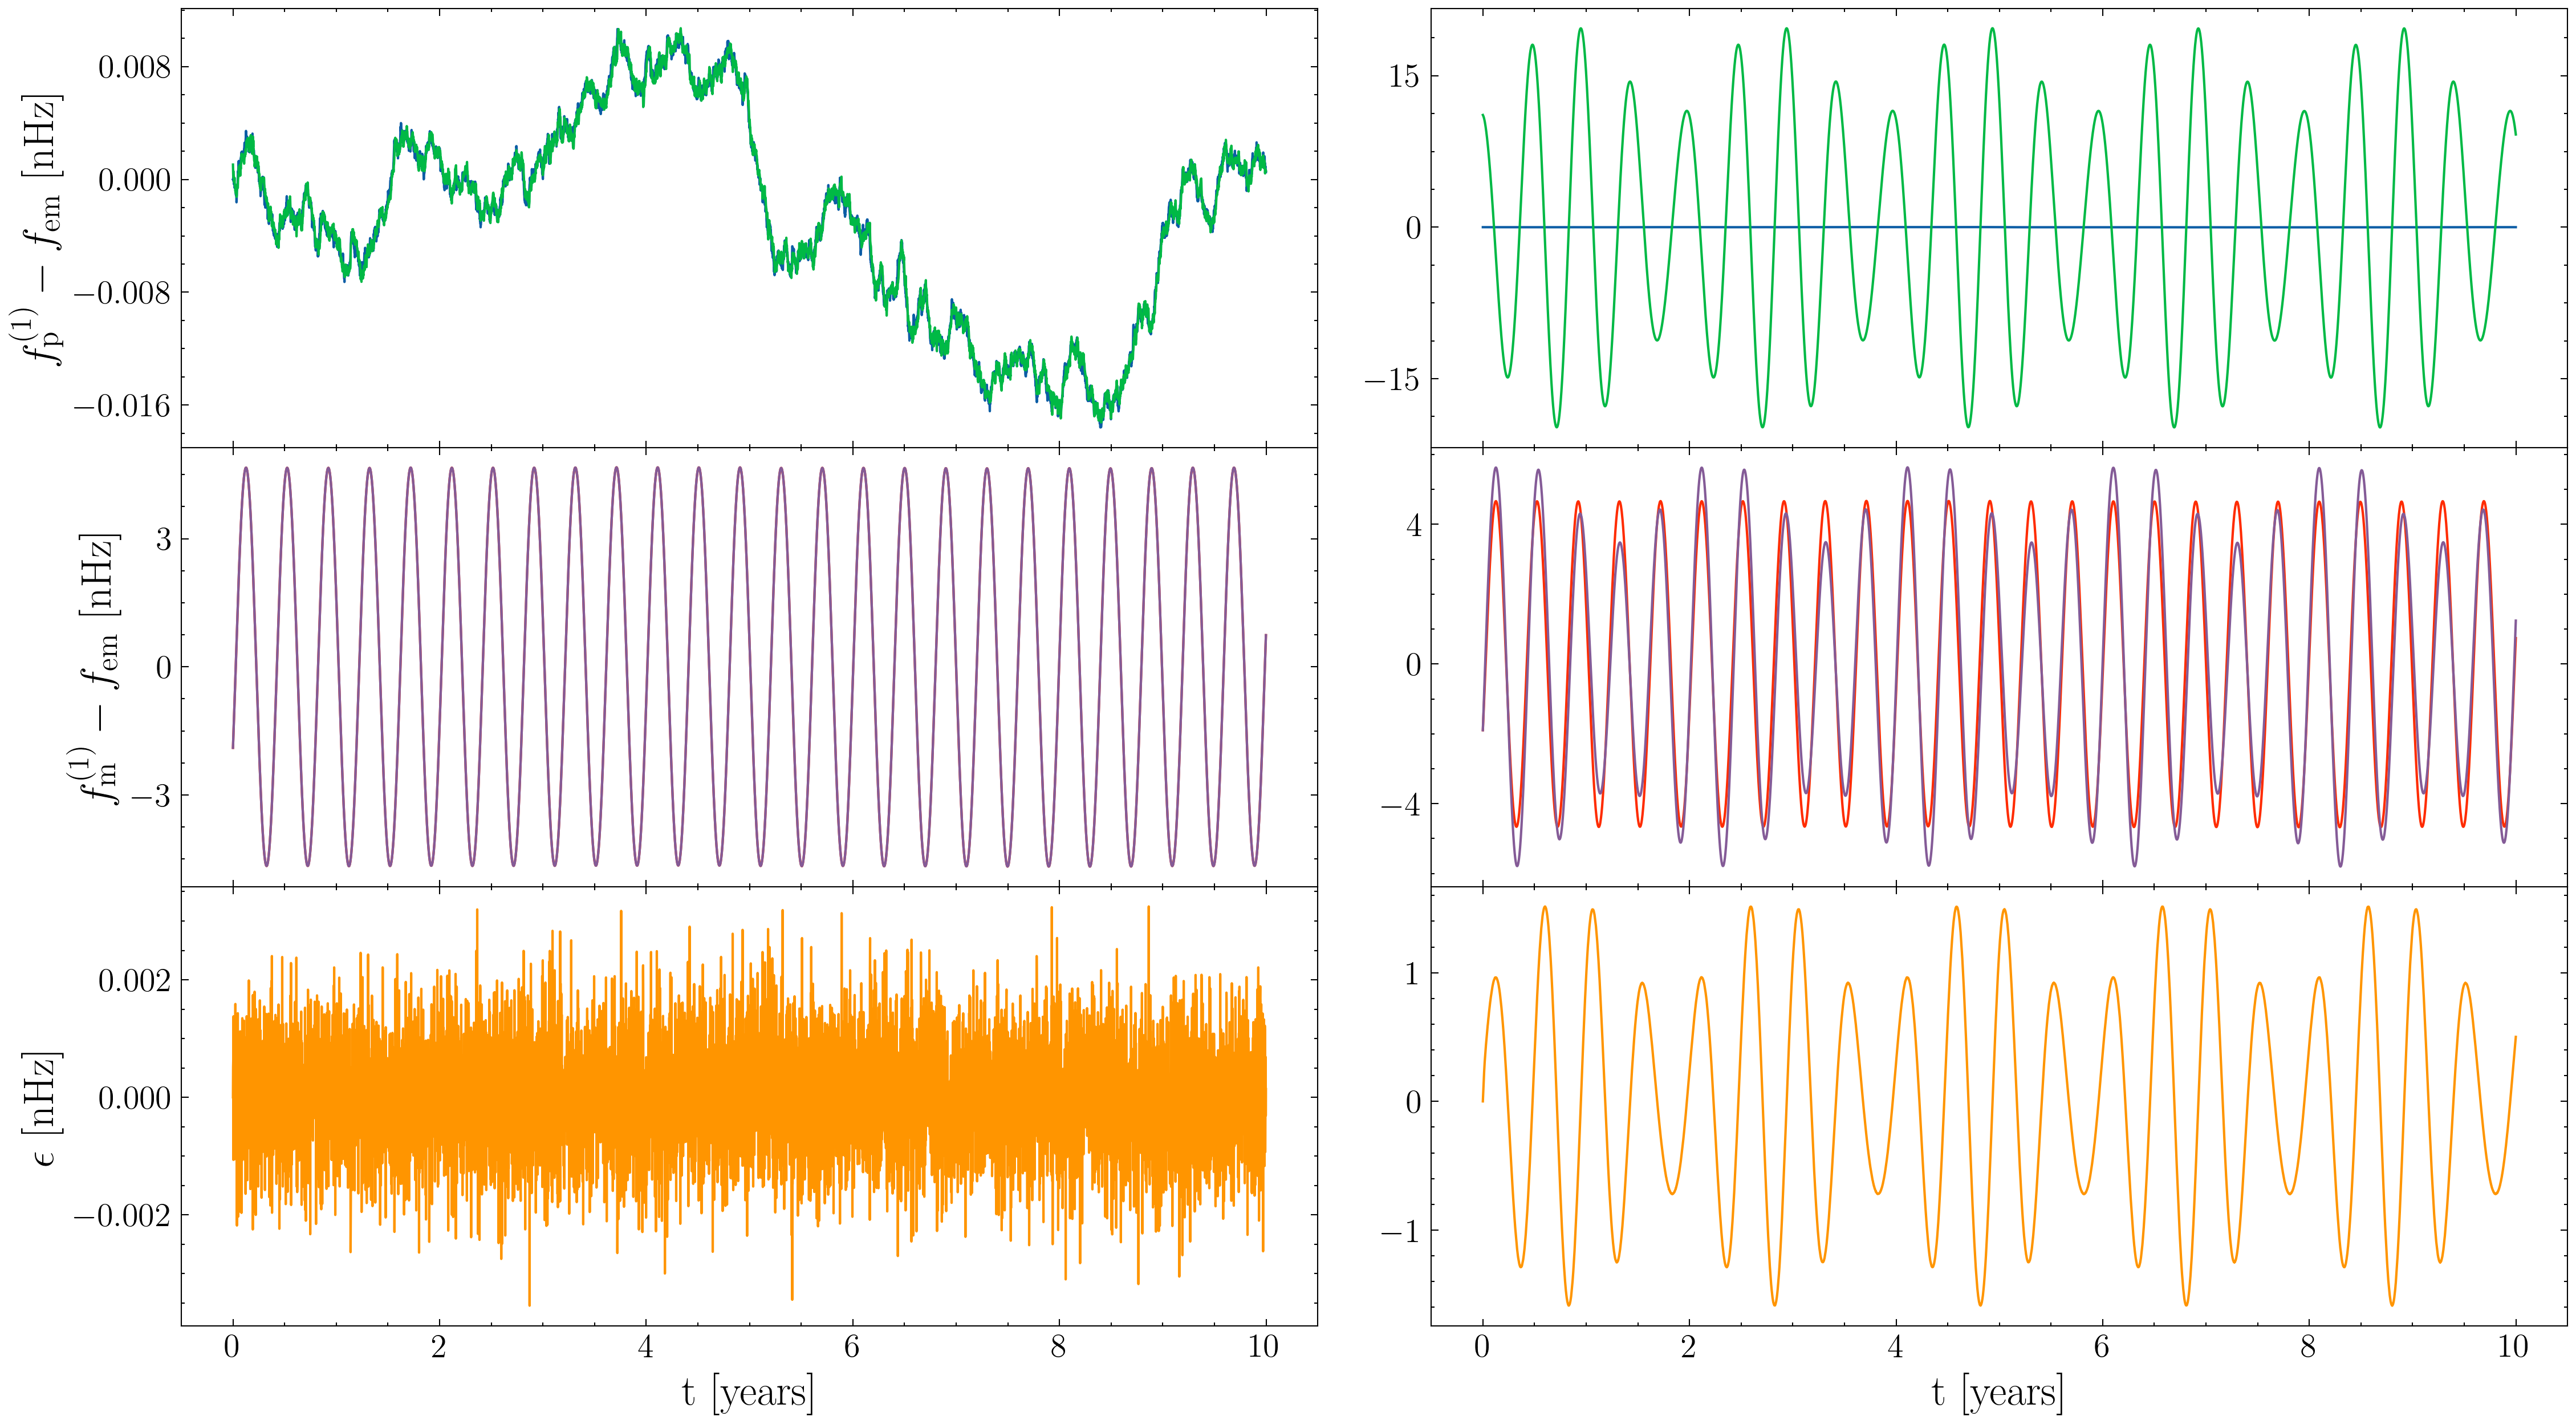
\includegraphics[width=0.5\textwidth]{images/Kalman_example_both}} 
%DIF < 	\subfloat[b]{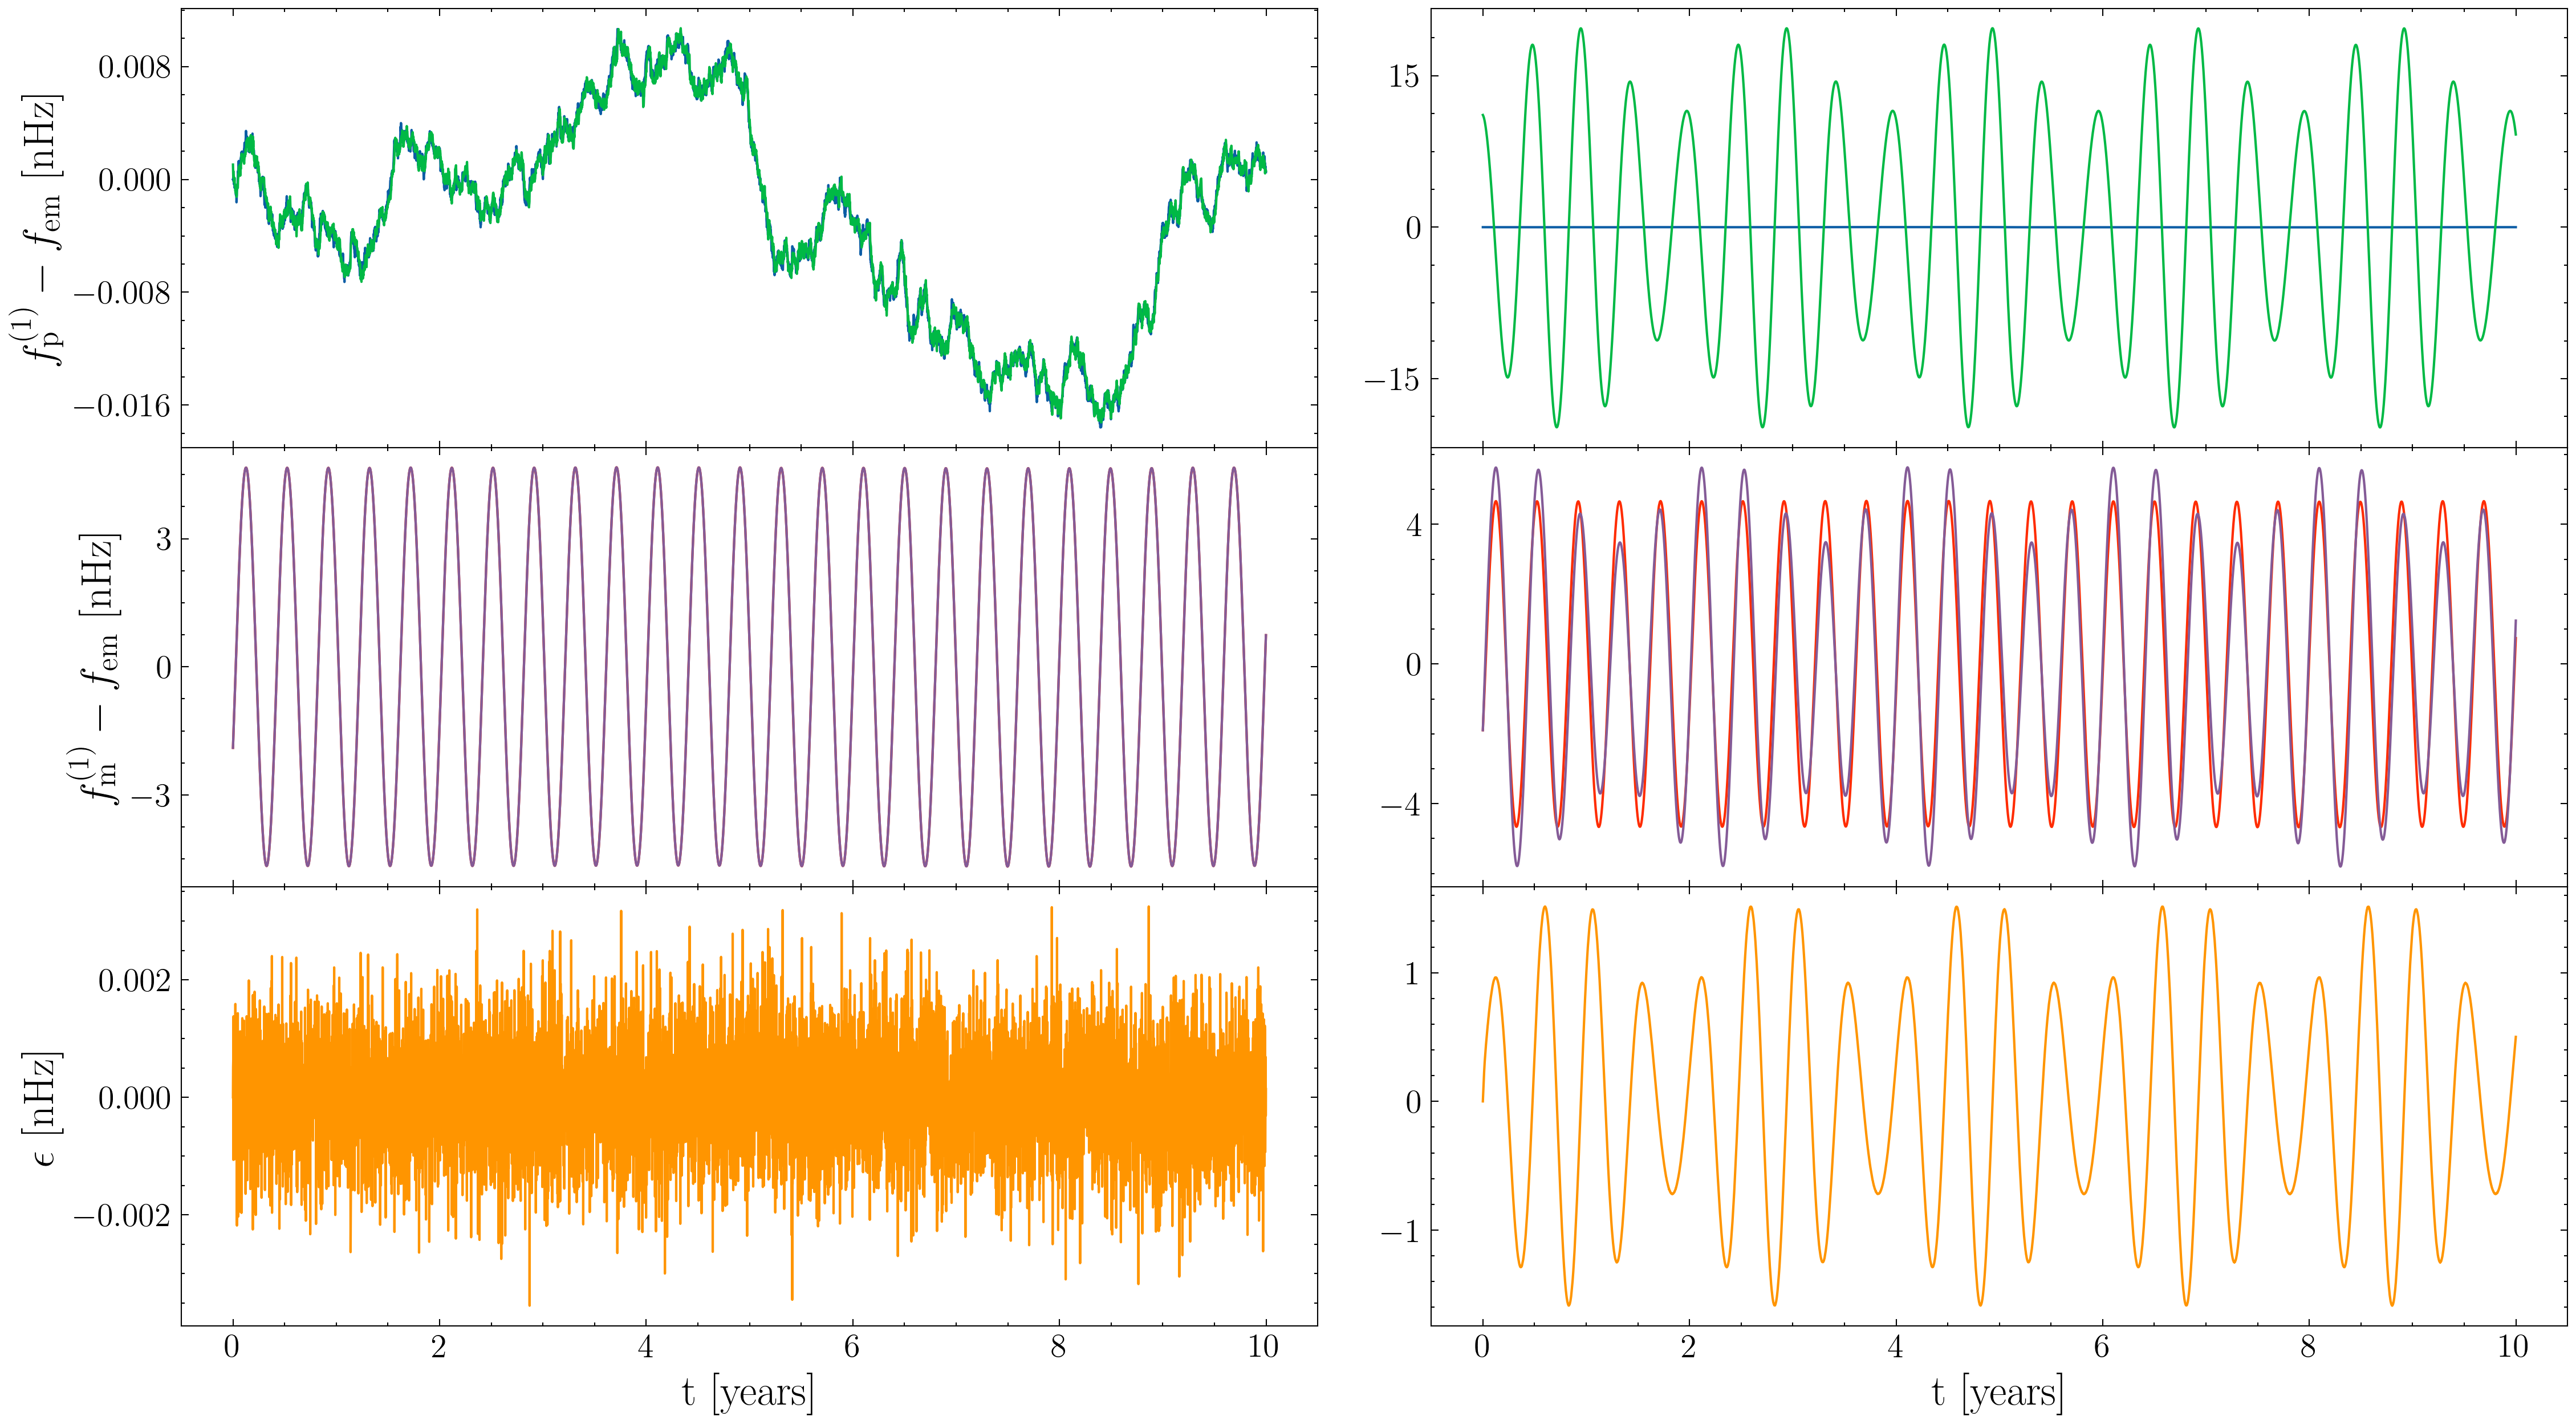
\includegraphics[width=0.3\textwidth]{images/Kalman_example_both}}
%DIF < 	\caption{\textcolor{red}{TK: For consideration. Do we prefer this figure to Figure \ref{fig:four figures}}?}
%DIF < 	\label{fig:kalmanexampleboth}
%DIF > 	%\centering % Not needed
%DIF > 	\begin{subfigure}[b]{0.49\textwidth}
%DIF > 		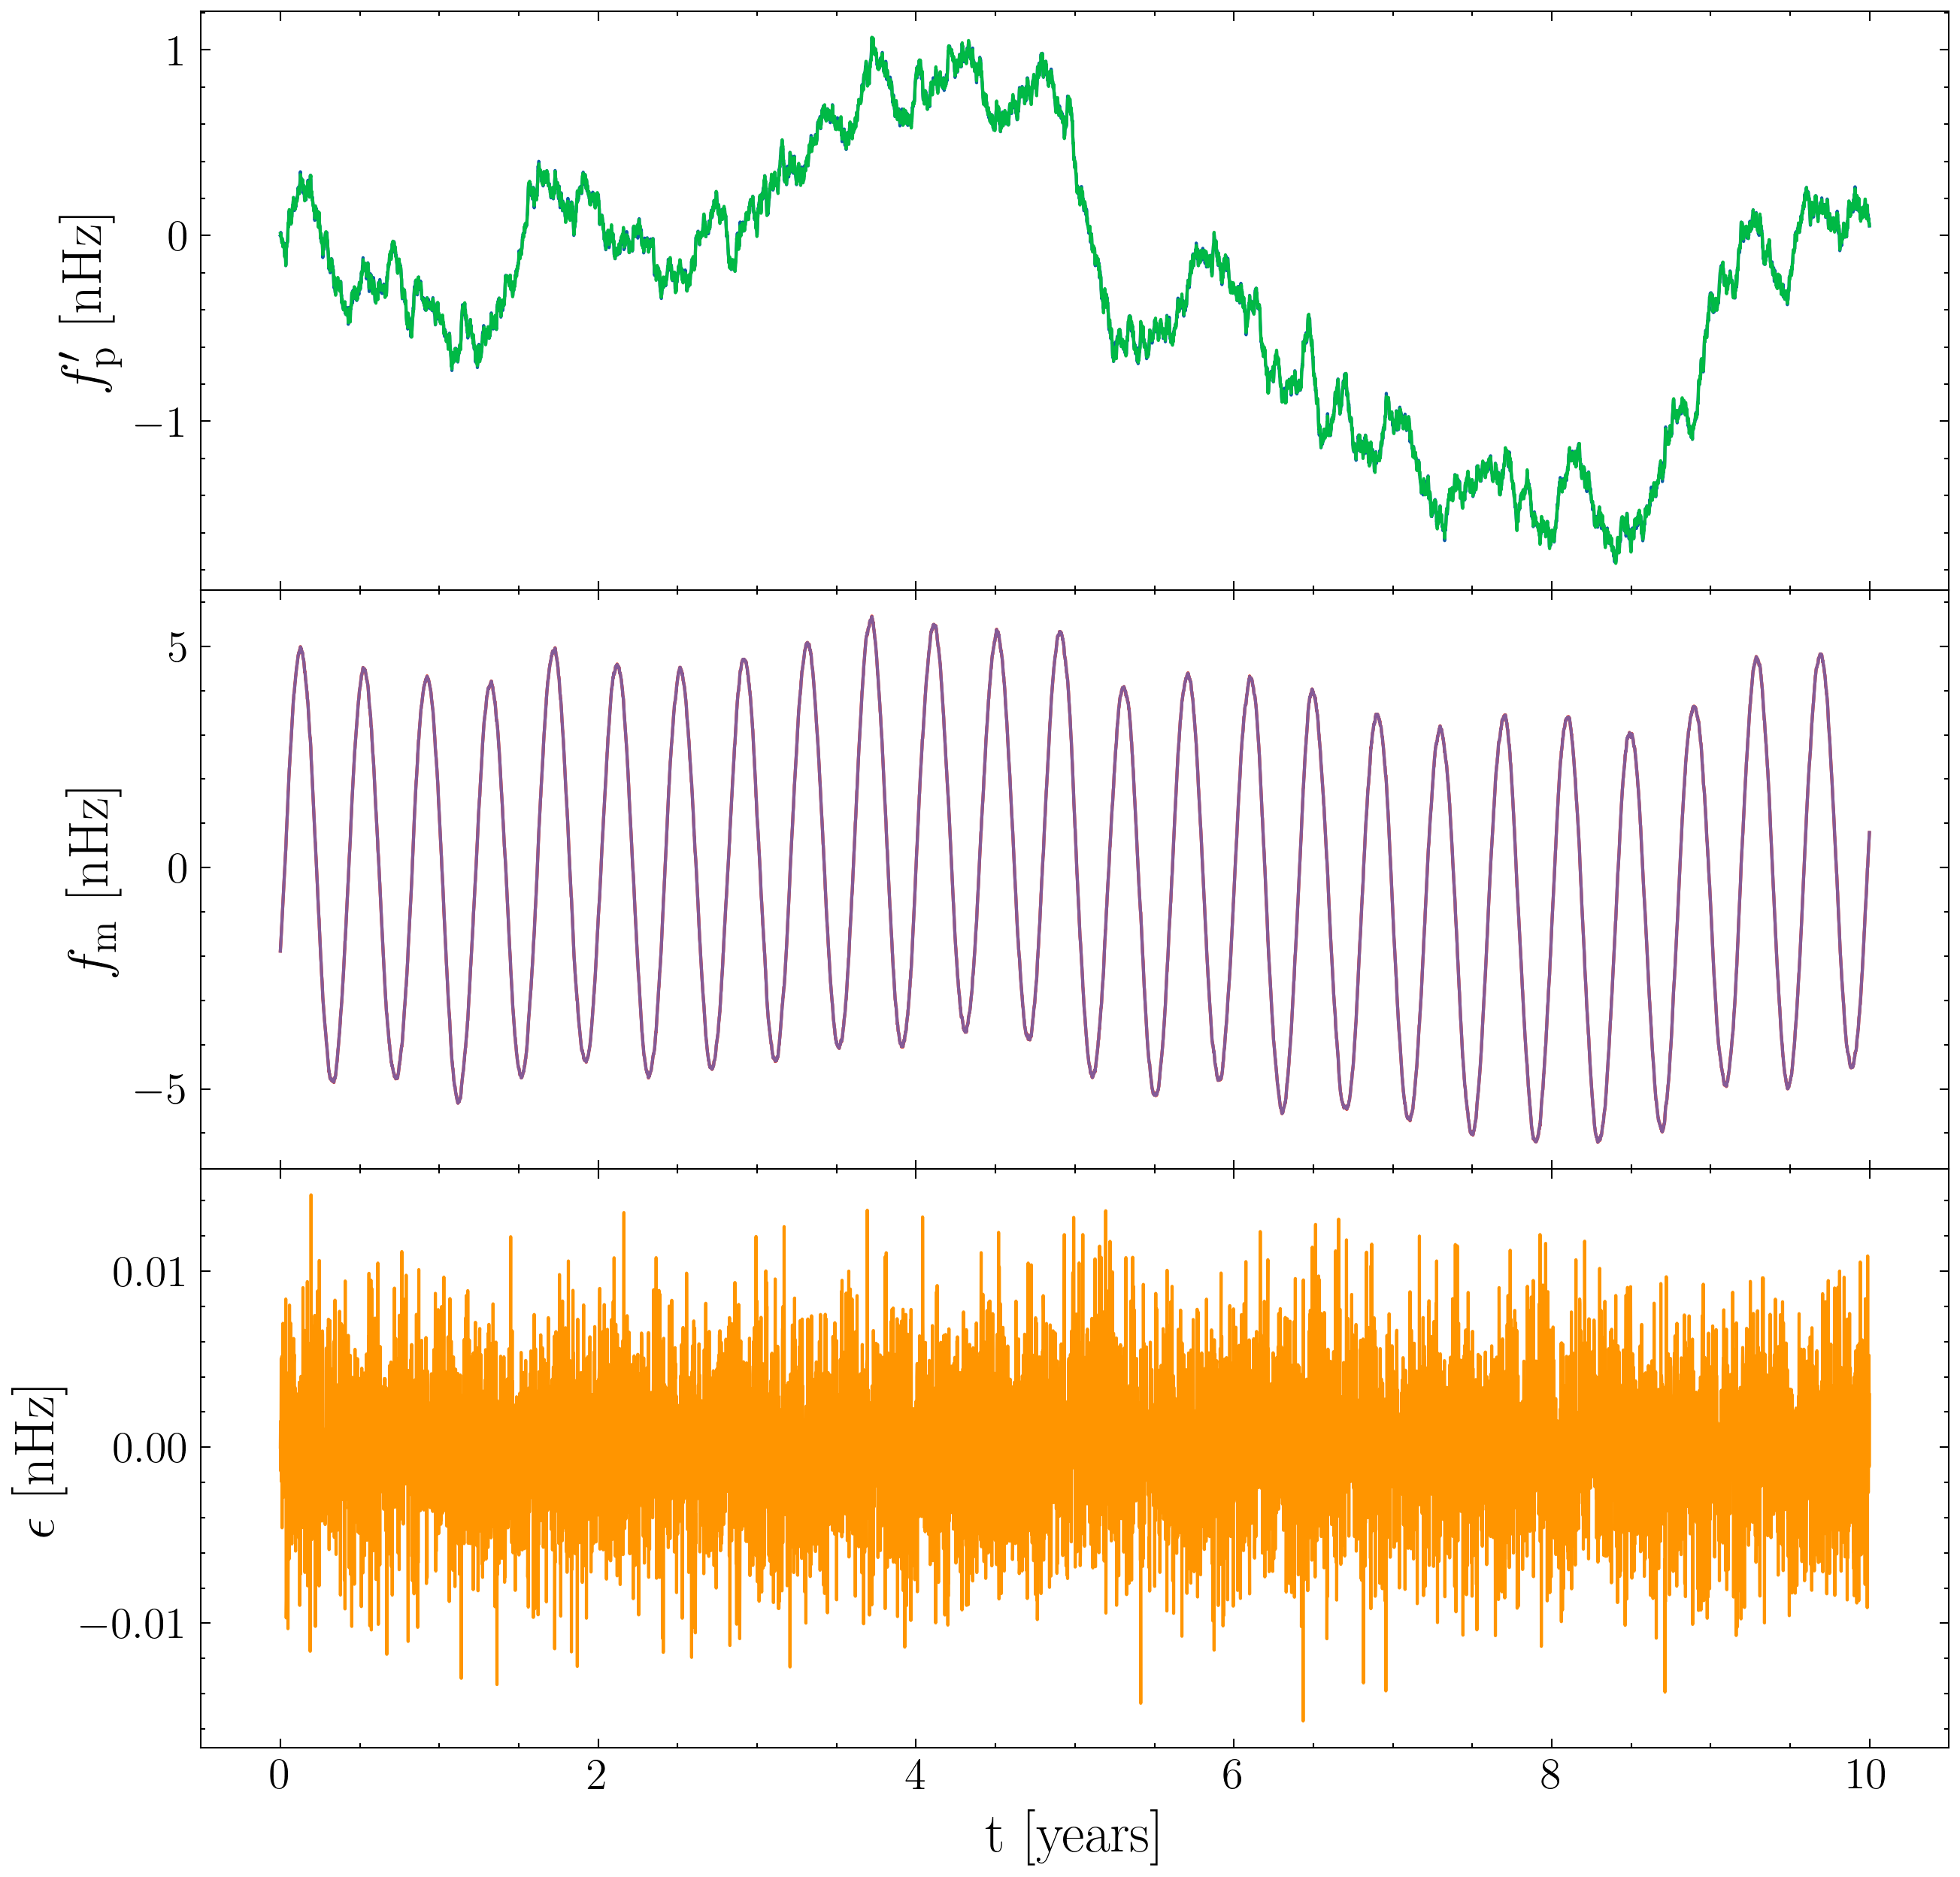
\includegraphics[width=\textwidth]{images/Kalman_example_true_params_single}
%DIF > 		\caption{Kalman filter using correct estimate of the static parameters, $\hat{\boldsymbol{\theta}} = \boldsymbol{\theta}$ }
%DIF > 		\label{fig:6MB_BFS}
%DIF > 	\end{subfigure}  
%DIF >     \hfill
%DIF > 	\begin{subfigure}[b]{0.49\textwidth}
%DIF > 		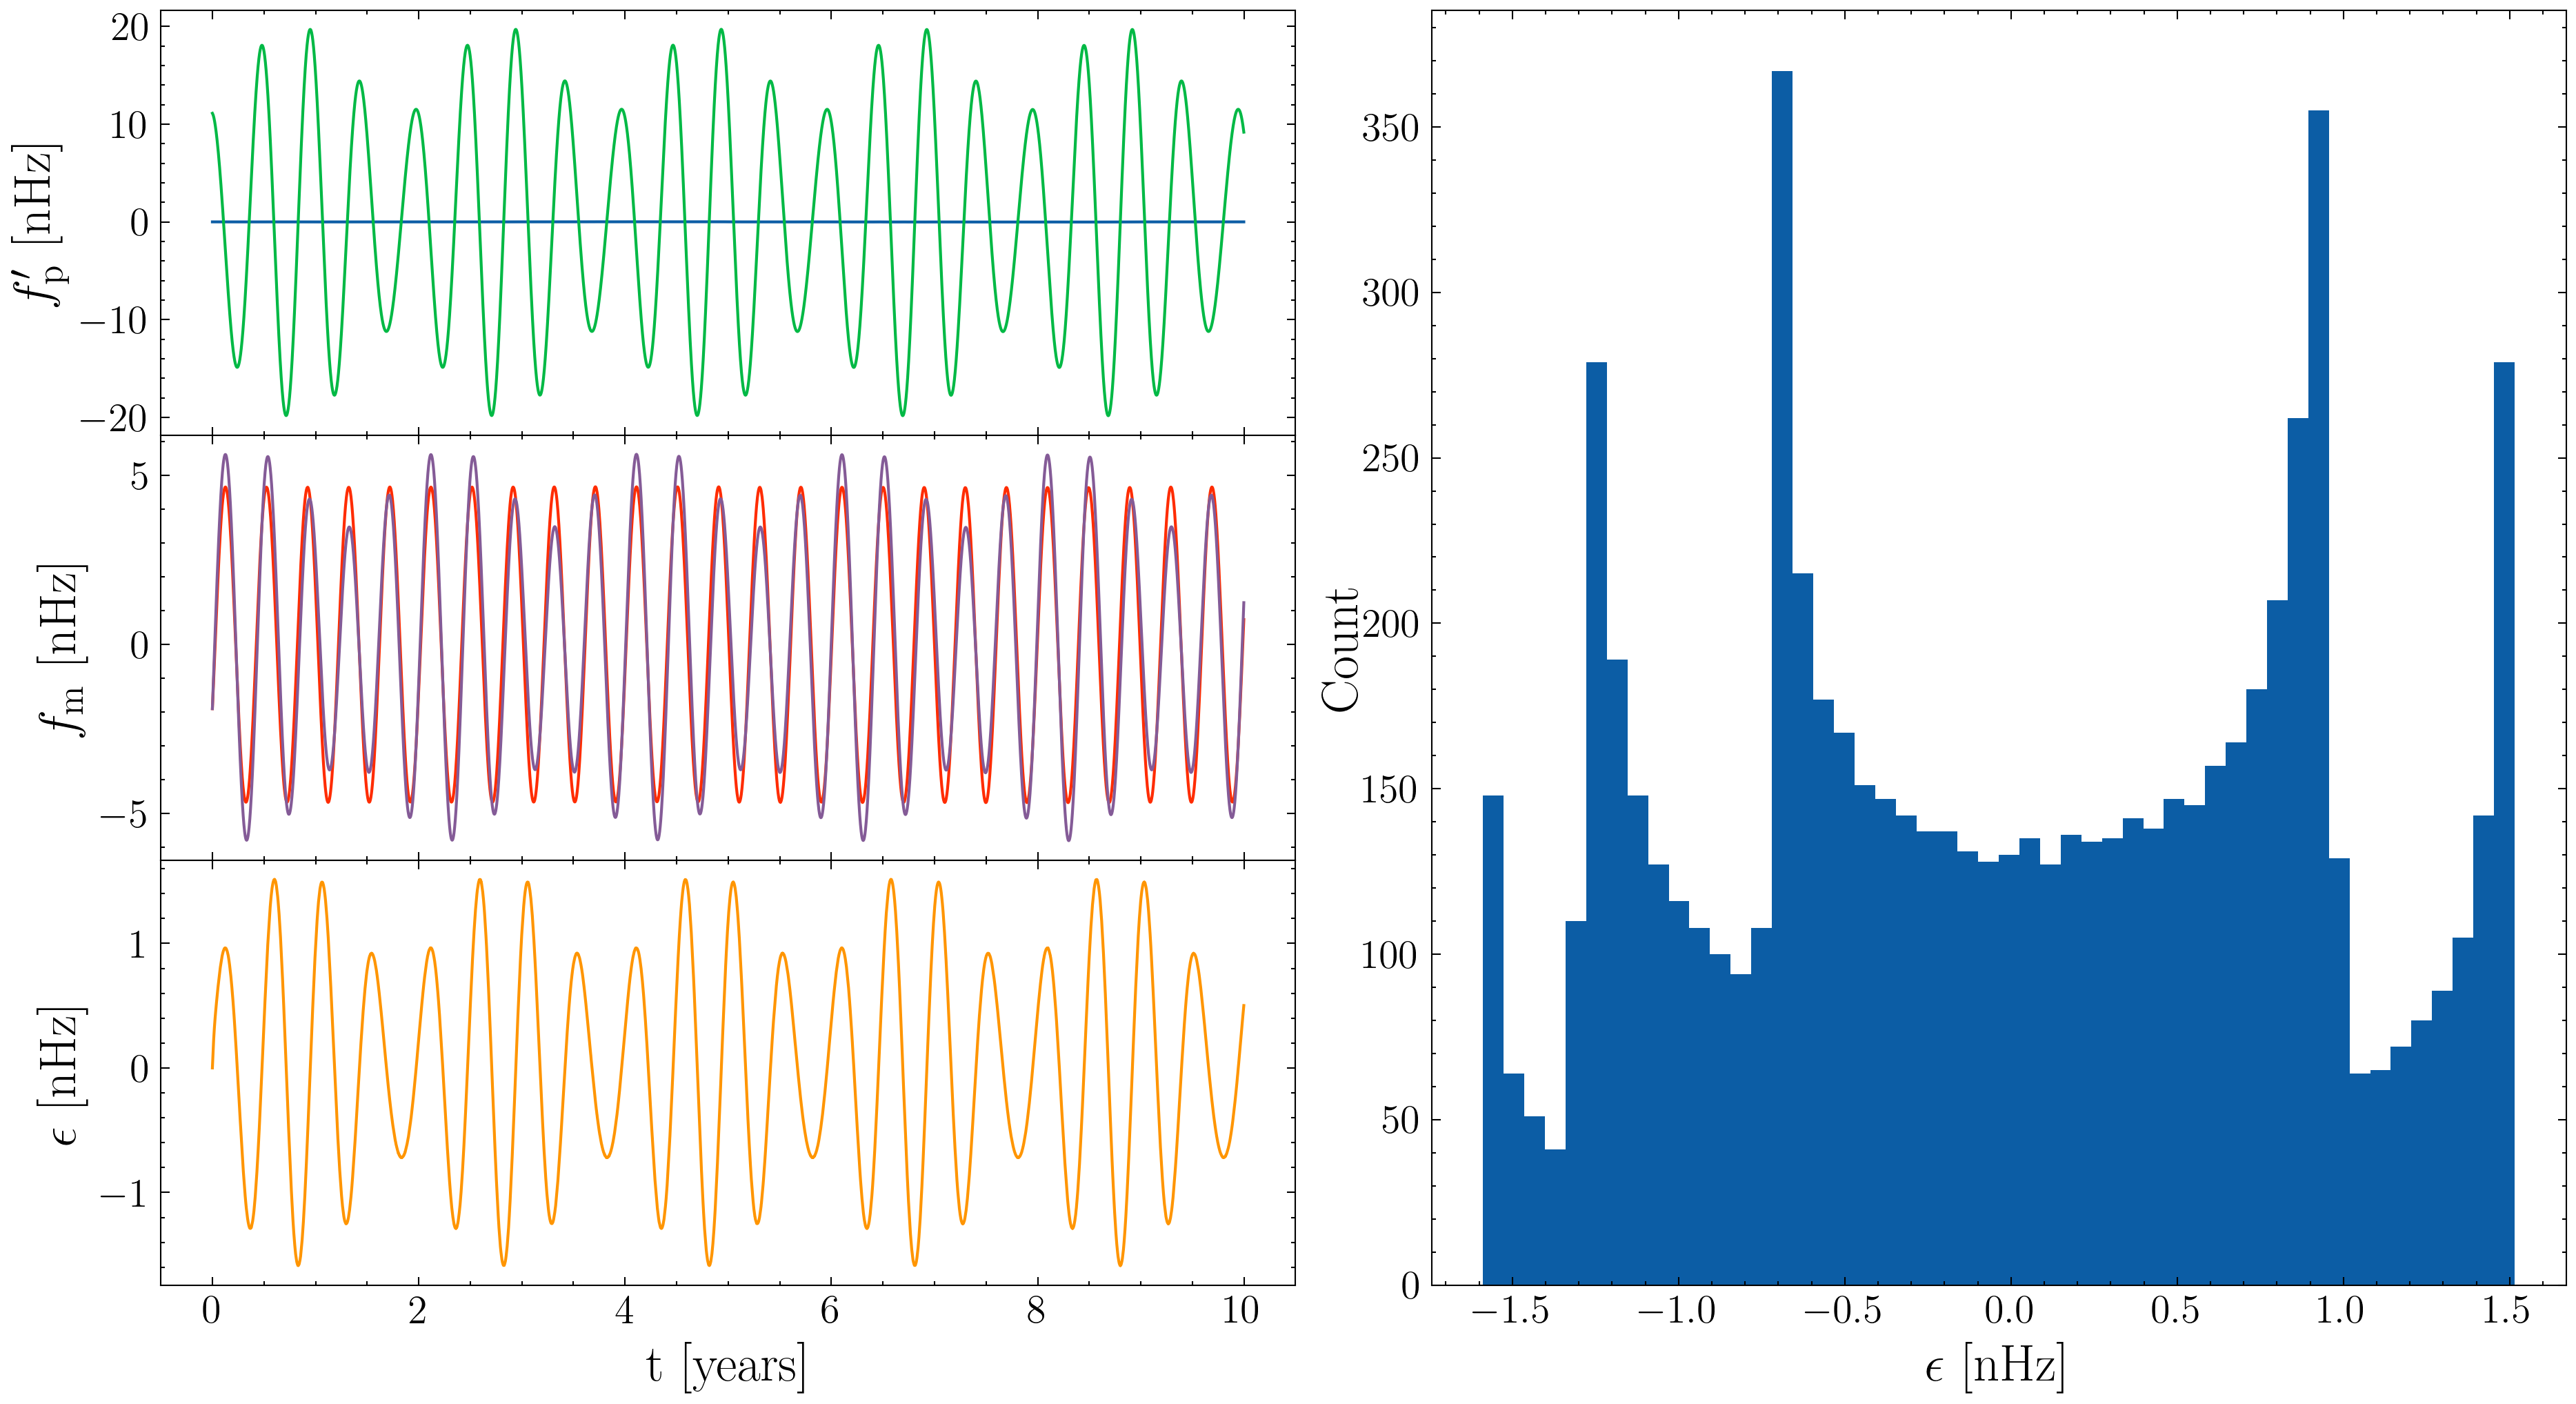
\includegraphics[width=\textwidth]{images/Kalman_example_wrong_params}
%DIF > 		\caption{Kalman filter using incorrect estimate of the static parameters, $\hat{\boldsymbol{\theta}} \neq \boldsymbol{\theta}$}
%DIF > 		\label{fig:25MB_bfs}
%DIF > 	\end{subfigure}
%DIF > 	\caption{
%DIF > 		}
%DIF > 	\label{fig:four figures}
%\end{figure*}
%DIF < 


\begin{figure*}
	%DIF < \centering % Not needed
	\DIFdelbeginFL %DIFDELCMD < \begin{subfigure}[b]{0.49\textwidth}
%DIFDELCMD < 		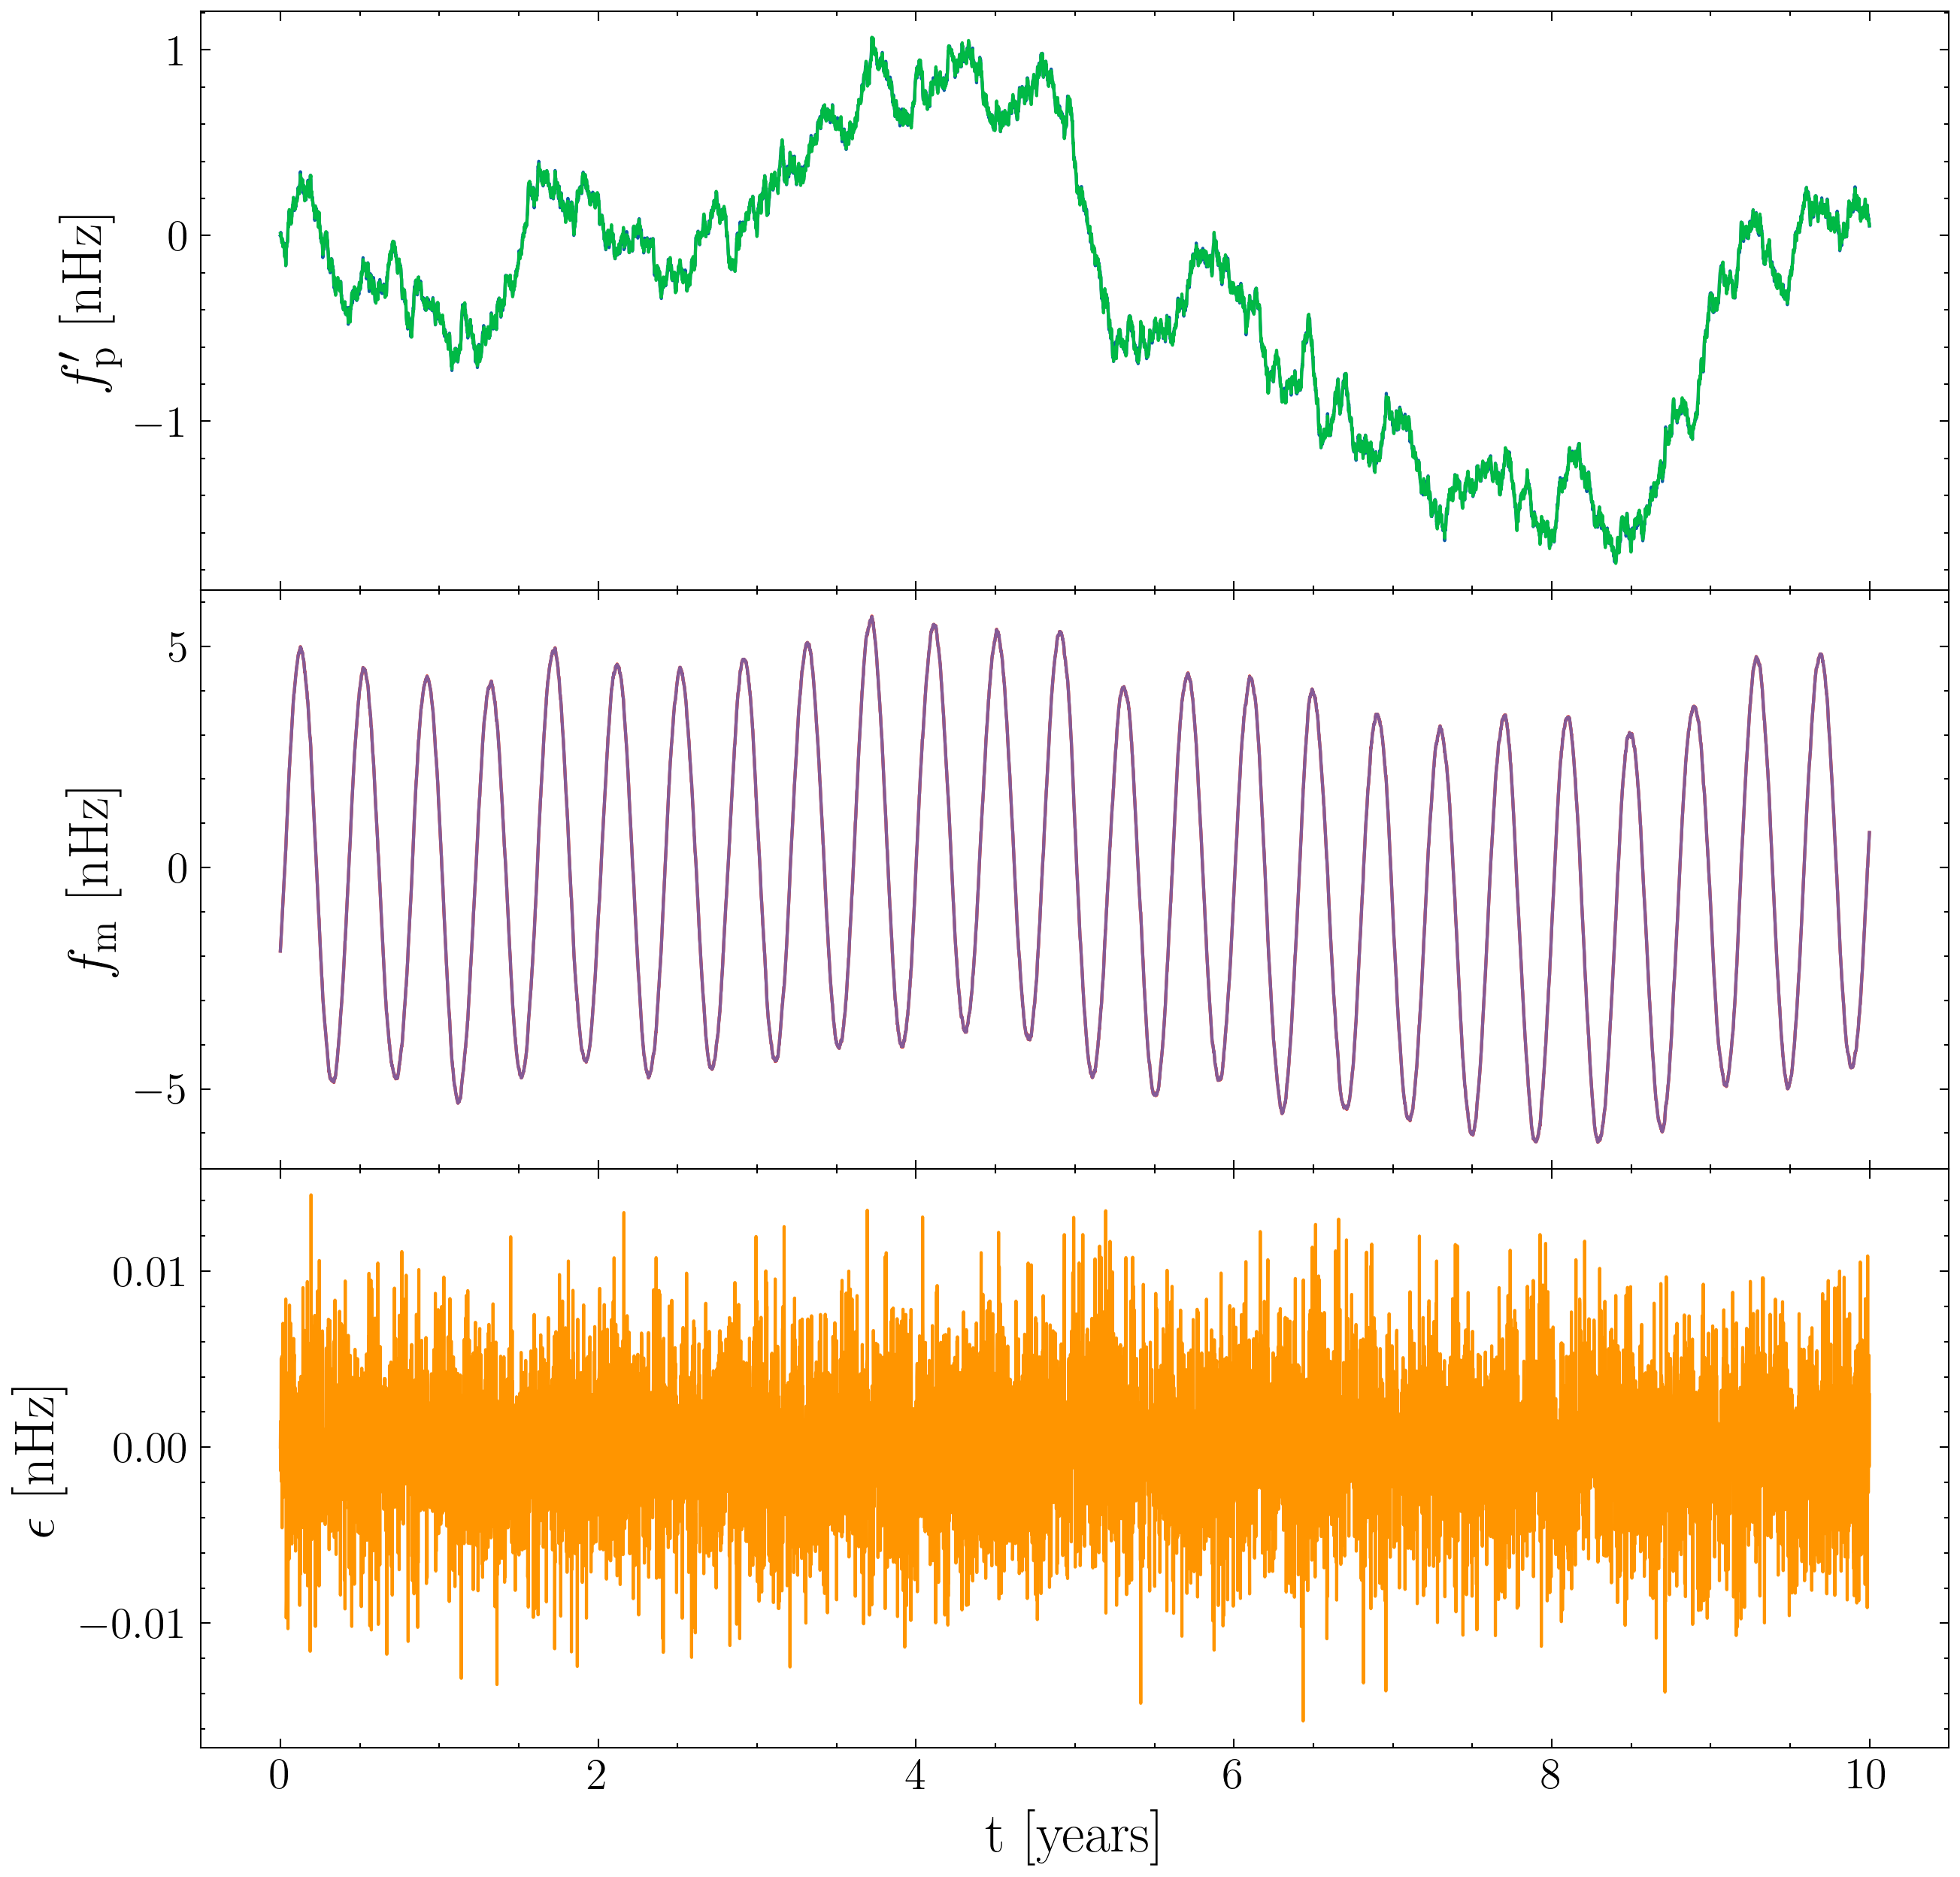
\includegraphics[width=\textwidth]{images/Kalman_example_true_params_single}
%DIFDELCMD < 		%%%
\DIFdelendFL \DIFaddbeginFL 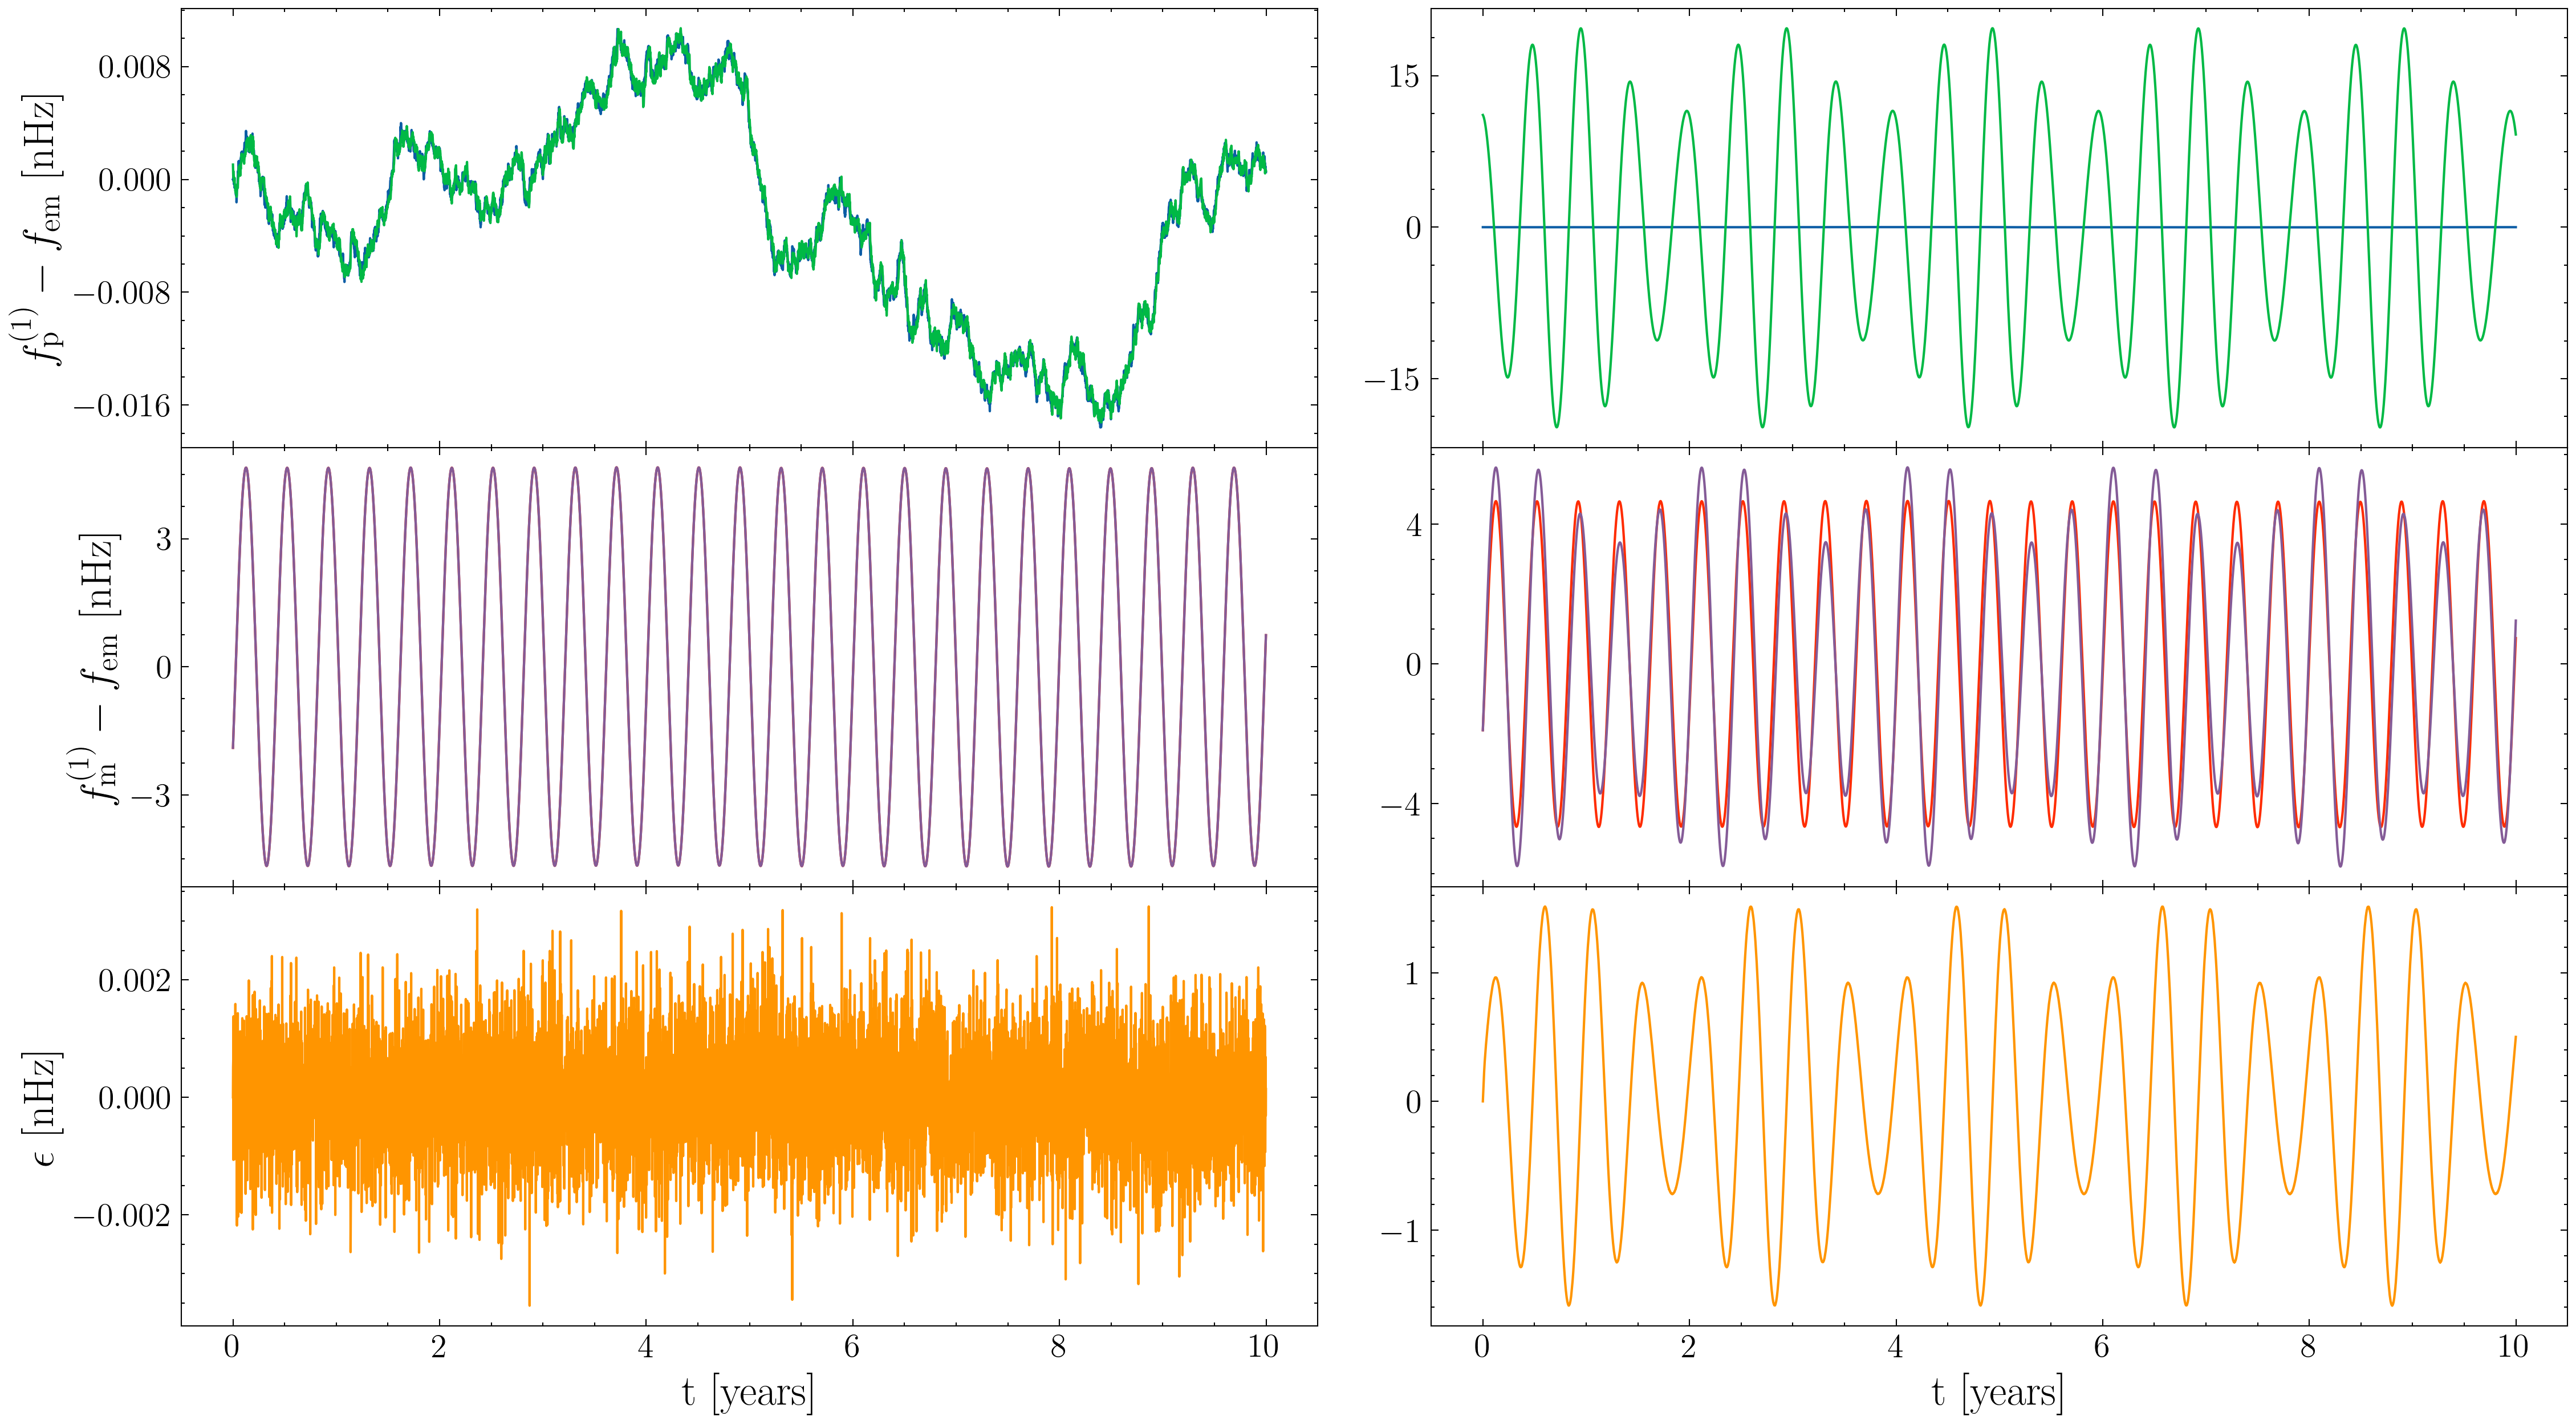
\includegraphics[width=\textwidth, height =0.5\textwidth]{images/Kalman_example_both}
	\DIFaddendFL \caption{\DIFaddbeginFL \DIFaddFL{Sample output of the }\DIFaddendFL Kalman filter \DIFdelbeginFL \DIFdelFL{using correct estimate }\DIFdelendFL \DIFaddbeginFL \DIFaddFL{illustrating the accuracy }\DIFaddendFL of the \DIFaddbeginFL \DIFaddFL{reconstructed systems state sequence $f_{\rm p}^{(1)}(t)$ when the }\DIFaddendFL static parameters \DIFaddbeginFL \DIFaddFL{are identically correct (${\boldsymbol{\hat\theta}} = {\boldsymbol{\theta}}$}\DIFaddendFL , \DIFdelbeginFL \DIFdelFL{$\hat{\boldsymbol{\theta}} = \boldsymbol{\theta}$ }\DIFdelendFL \DIFaddbeginFL \DIFaddFL{left column) and incorrect (${\boldsymbol{\hat\theta}} \neq {\boldsymbol{\theta}}$, right column). The top panels show the true pulsar state $f_{\rm p}^{1}(t) - f_{\rm em}^{(1)}(t)$ (blue curve) and the state estimated by the Kalman filter $\hat{f}_{\rm p}^{1}(t) - f_{\rm em}^{(1)}(t)$  (green curve). We plot the subtracted state to better illustrate the stochastic wandering of the pulsar frequency. In the left hand column, the blue/green solutions are completely overlaid. The middle panels show the true measured frequency $f_{\rm m}^{1}(t) - f_{\rm em}^{(1)}(t)$ (red curve) and the frequency estimated  by the Kalman filter $\hat{f}_{\rm m}^{1}(t) - f_{\rm em}^{(1)}(t)$ (magenta curve). Again we plot the subtracted state, and in the left hand column the red/magenta solutions are completely overlaid. The bottom panels show the residual or the innovation $\epsilon(t) =f_{\rm m}^{1}(t) - \hat{f}_{\rm m}^{1}(t)$. The results are shown for a single pulsar. In the right hand column $\Omega$ has been perturbed from its true value by 20\%}\DIFaddendFL } 
	\DIFdelbeginFL %DIFDELCMD < \label{fig:6MB_BFS}
%DIFDELCMD < 	\end{subfigure}  
%DIFDELCMD <     \hfill
%DIFDELCMD < 	\begin{subfigure}[b]{0.49\textwidth}
%DIFDELCMD < 		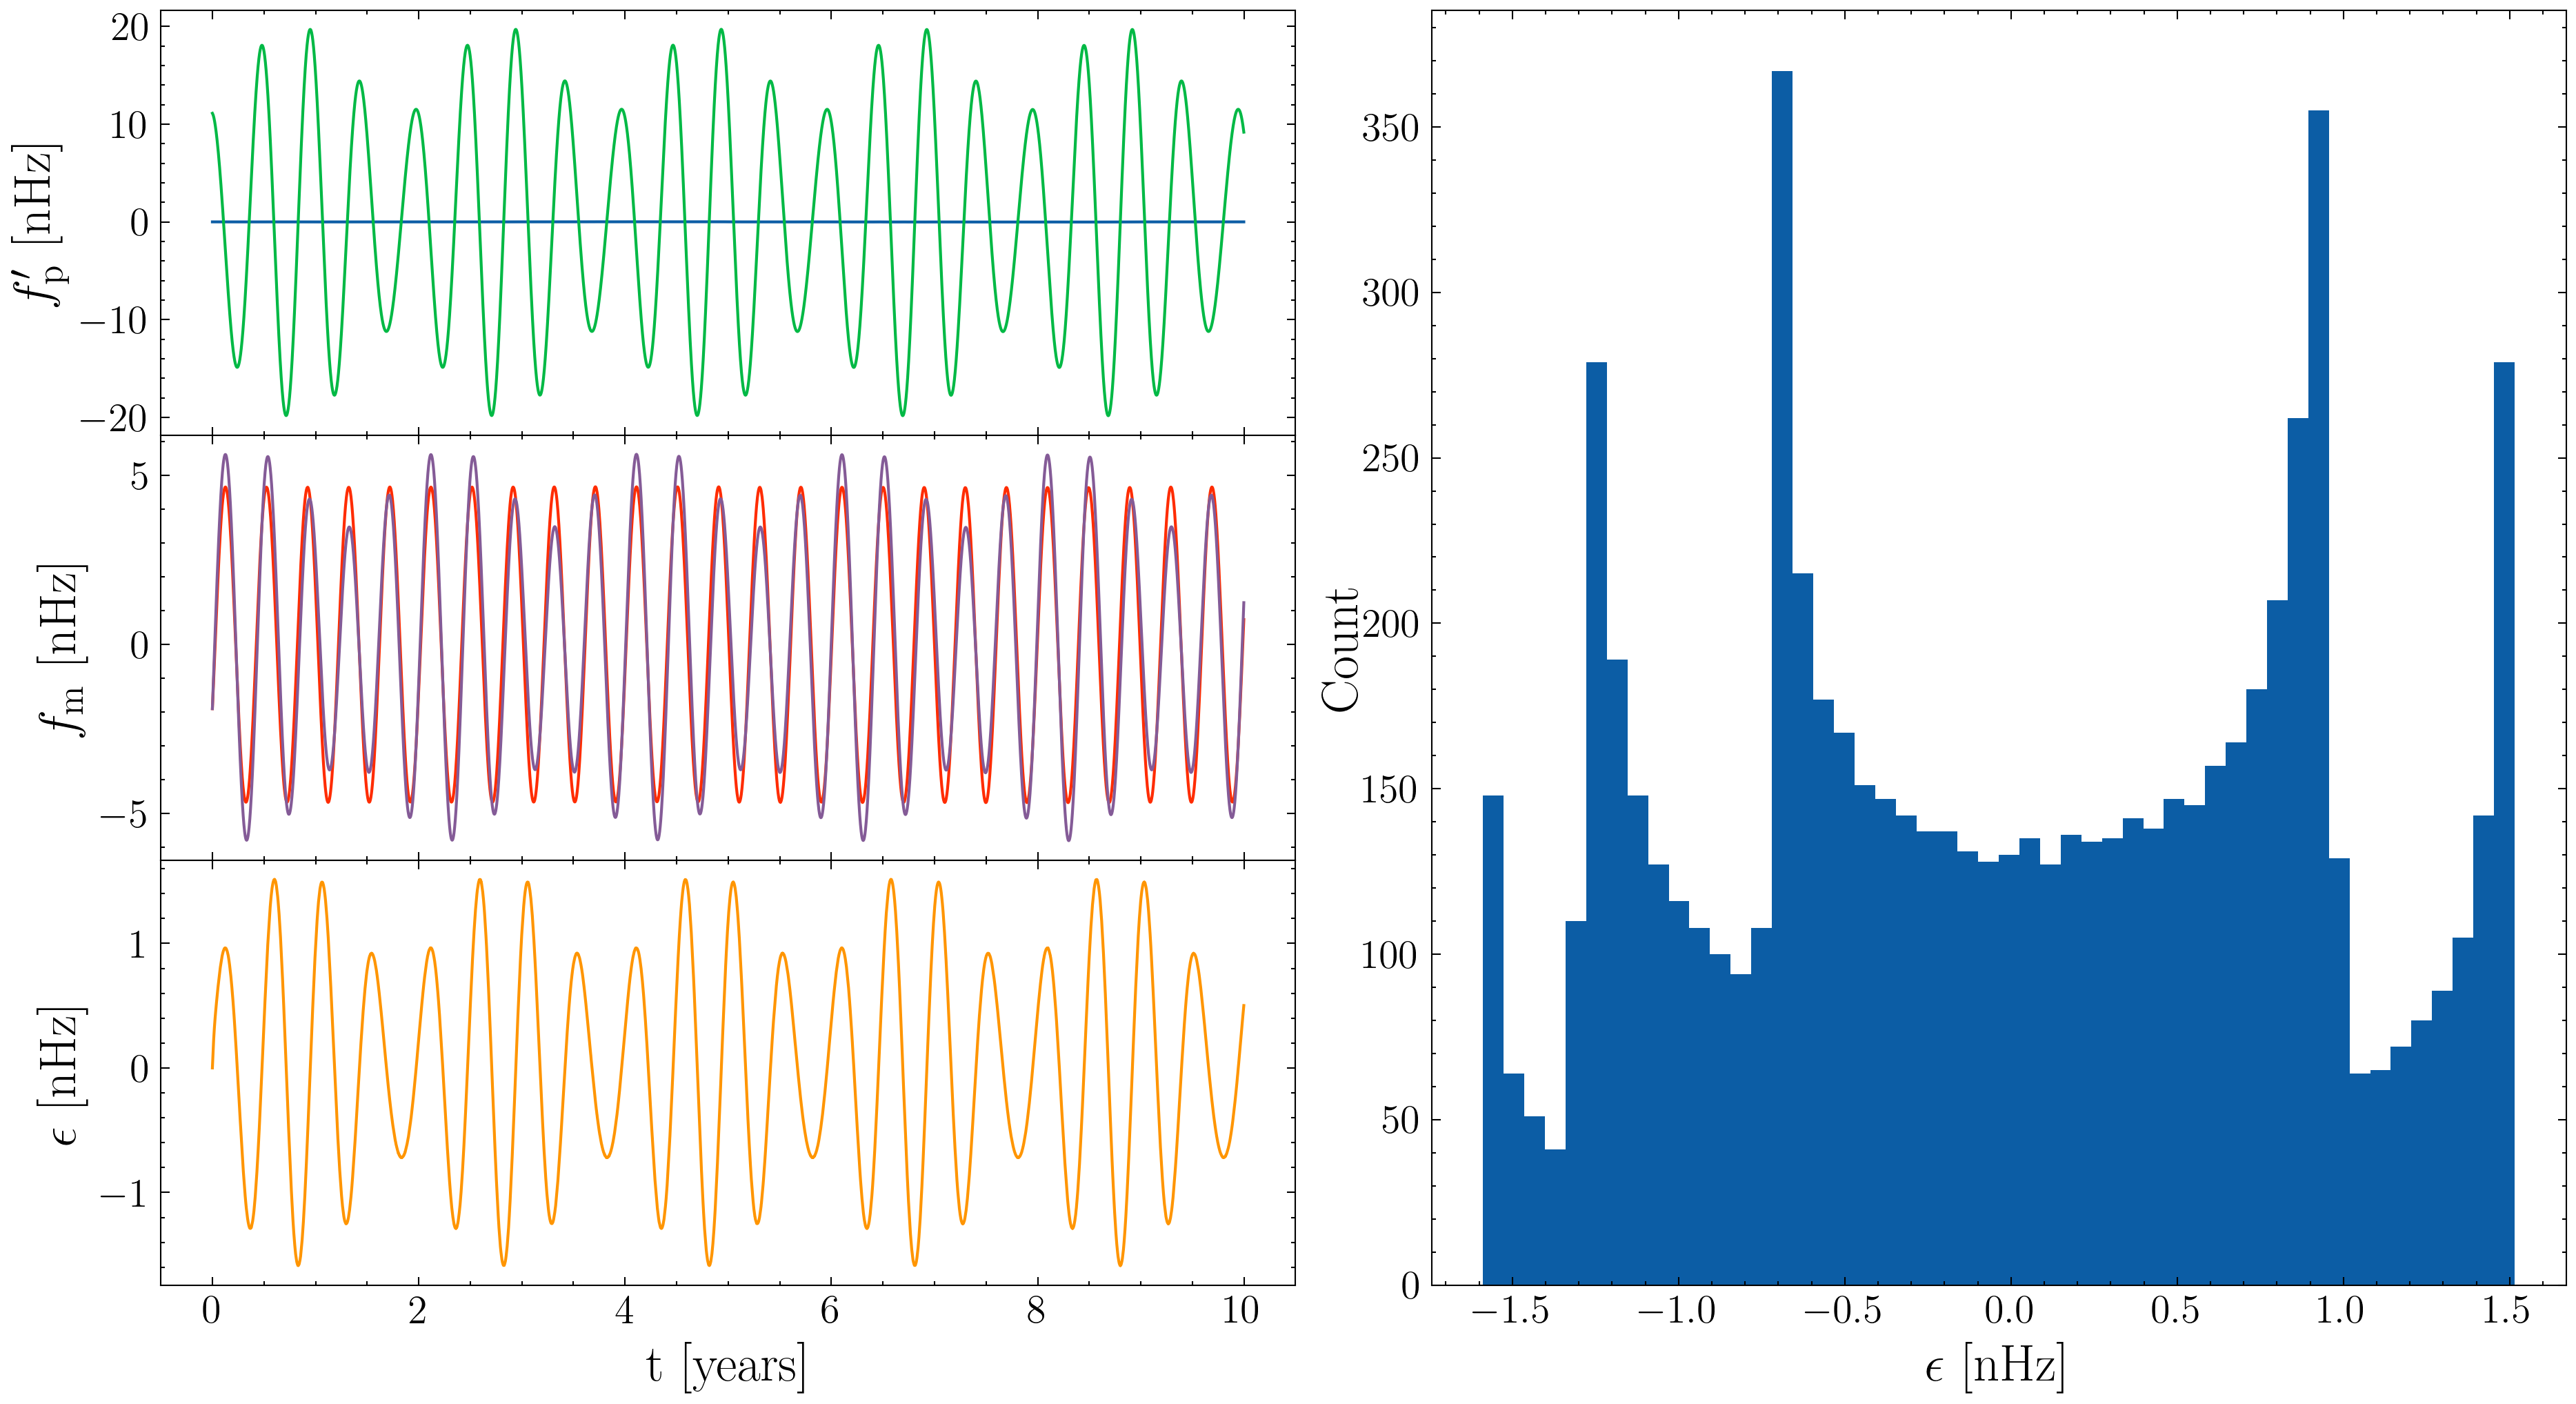
\includegraphics[width=\textwidth]{images/Kalman_example_wrong_params}
%DIFDELCMD < 		%%%
%DIFDELCMD < \caption{%
{%DIFAUXCMD
\DIFdelFL{Kalman filter using incorrect estimate of the static parameters, $\hat{\boldsymbol{\theta}} \neq \boldsymbol{\theta}$}}
		%DIFAUXCMD
%DIFDELCMD < \label{fig:25MB_bfs}
%DIFDELCMD < 	\end{subfigure}
%DIFDELCMD < 	%%%
%DIFDELCMD < \caption{%
{%DIFAUXCMD
\DIFdelFL{Example application of a Kalman filter to estimate the intrinsic pulsar frequency state $f_{\rm p}(t)$ given a measured frequency $f_{\rm m}(t)$. We plot the ephemeris subtracted state $f'_{\rm p}(t) = f_{\rm p}(t) - f_{\rm em} (t)$ to better illustrate the stochastic wandering of the pulsar frequency. In (a) the Kalman filter is run using identically correct estimates of the static system parameters, $\hat{\boldsymbol{\theta}} = \boldsymbol{\theta}$ and the state is estimated accurately. In (b) the Kalman filter is run with $\hat{\boldsymbol{\theta}} \neq \boldsymbol{\theta}$ and the state is not estimated accurately. The top panels show the true pulsar state $f'_{\rm p}(t)$ (blue line) and the state estimated by the Kalman filter, $\hat{f'}_{\rm p}(t)$ (green line). The middle panels show the true $f_{\rm m}(t)$ (red line) and the measured frequency estimated  by the Kalman filter, $\hat{f}_{\rm m}(t)$ (magenta). The bottom panels show the residual or the innovation $\epsilon(t) =f_{\rm m}(t) - \hat{f}_{\rm m}(t)$. In (a) the green/blue and red/magenta lines are completely overlaid.}}
	%DIFAUXCMD
%DIFDELCMD < \label{fig:four figures}
%DIFDELCMD < %%%
\DIFdelendFL \DIFaddbeginFL \label{fig:kalman_example}
\DIFaddendFL \end{figure*}


The Kalman filter \citep{Kalman1} is a \DIFdelbegin \DIFdel{Gaussian-Markov }\DIFdelend \DIFaddbegin \DIFadd{Gauss-Markov }\DIFaddend model used to algorithmically recover \DIFdelbegin \DIFdel{the most likely set of unknown }\DIFdelend \DIFaddbegin \DIFadd{a temporal sequence of stochastically evolving  }\DIFaddend system state variables, \DIFdelbegin \DIFdel{$\boldsymbol{X}$, given some }\DIFdelend \DIFaddbegin \DIFadd{$\boldsymbol{X}(t)$, which are not observed directly, given a temporal sequence of }\DIFaddend noisy measurements, \DIFdelbegin \DIFdel{$\boldsymbol{Y}$. It is a common technique in signal processing that }\DIFdelend \DIFaddbegin \DIFadd{$\boldsymbol{Y}(t)$. It finds common use in engineering applications and }\DIFaddend has been applied successfully in neutron star astrophysics \DIFdelbegin \DIFdel{\mbox{%DIFAUXCMD
\citep[e.g.][]{Meyers2021,Melatos2023}}\hskip0pt%DIFAUXCMD
}\DIFdelend \DIFaddbegin \DIFadd{\mbox{%DIFAUXCMD
\citep[e.g.][]{Myers2021MNRAS.502.3113M,Meyers2021,Melatos2023}}\hskip0pt%DIFAUXCMD
}\DIFaddend . In this work we use the linear Kalman filter\DIFaddbegin \DIFadd{, }\DIFaddend which assumes a linear relation between \DIFdelbegin \DIFdel{$\boldsymbol{X}$ and $\boldsymbol{Y}$. Whilst the measurement equation, Equation \eqref{eq:measurement}, is non-linear in the static parameters it is linear in the state and measurement variables, $f_{\rm p}^{(n)}$ and $f_{\rm m}^{(n)}$ respectively}\DIFdelend \DIFaddbegin \DIFadd{$d{\boldsymbol{X}}/dt$ and ${\boldsymbol{X}}(t)$ (dynamics) and between ${\boldsymbol{Y}}(t)$ and ${\boldsymbol{X}}(t)$ (measurement), with ${\boldsymbol{X}}(t) = \{ f_{\rm p}^{(n)}(t) \}$ and ${\boldsymbol{Y}}(t) = \{ f_{\rm m}^{(n)}(t) \}$}\DIFaddend . Extension to non-linear problems is straightforward using either an extended Kalman filter \citep{zarchan2000fundamentals}, \DIFdelbegin \DIFdel{the }\DIFdelend unscented Kalman filter \citep{882463van} or \DIFdelbegin \DIFdel{the }\DIFdelend particle filter \citep{Simon10}. \DIFaddbegin \DIFadd{Equations \eqref{eq:measurement} and \eqref{eq:g_func} are non-linear in the static parameters (e.g.\ $d^{(n)}$), even though they are linear in ${\boldsymbol{X}}(t)$ and ${\boldsymbol{Y}}(t)$. Hence inferring the static parameters is a non-linear exercise, to be tackled separately after the linear Kalman filter operates on the data for a fixed set of static parameters. Inference of the static parameters in Equations \eqref{eq:measurement} and \eqref{eq:g_func} by nested sampling is discussed in Section \ref{sec:nested_sampling}. }\DIFaddend \newline 

\DIFdelbegin \DIFdel{The }\DIFdelend \DIFaddbegin \DIFadd{Implementation of the linear Kalman filter for the PTA state-space model in Section 3.2, including the }\DIFaddend full set of Kalman \DIFdelbegin \DIFdel{recursions }\DIFdelend \DIFaddbegin \DIFadd{recursion relations }\DIFaddend is presented in Appendix \ref{sec:kalman}. At each discrete timestep indexed by $ 1 \leq i  \leq M$, the Kalman filter returns an estimate of the state variables, \DIFdelbegin \DIFdel{$\hat{\boldsymbol{X}}_i$}\DIFdelend \DIFaddbegin \DIFadd{$\hat{\boldsymbol{X}}_i = \hat{\boldsymbol{X}}(t_i)$}\DIFaddend , and the covariance of those estimates, \DIFdelbegin \DIFdel{$\boldsymbol{P}_i$}\DIFdelend \DIFaddbegin \DIFadd{${\boldsymbol{P}}_i = \langle {\boldsymbol{\hat X}}_i {\boldsymbol{\hat X}}_i^{\rm T} \rangle$, where the superscript T denotes the matrix transpose}\DIFaddend . The filter tracks the error in its predictions of $\boldsymbol{X}_i$ by \DIFdelbegin \DIFdel{projecting the state predictions back into measurement space, $\hat{\boldsymbol{X}}_i \mapsto \hat{\boldsymbol{Y}}_i$, via the measurement equation, Equation \eqref{eq:measurement} . The measurement predictions can then be compared against the true observed noisy measurements to get }\DIFdelend \DIFaddbegin \DIFadd{converting ${\boldsymbol{\hat X}}_i$ into predicted measurements ${\boldsymbol{\hat Y}}_i$ via Equations \eqref{eq:measurement} and \eqref{eq:g_func} and comparing with the actual, noisy measurements ${\boldsymbol{\hat Y}}_i$. This defines }\DIFaddend a residual $\boldsymbol{\epsilon}_i = \boldsymbol{Y}_i  - \hat{\boldsymbol{Y}}_i$, \DIFaddbegin \DIFadd{which is }\DIFaddend sometimes termed the \DIFdelbegin \DIFdel{``innovation"}\DIFdelend \DIFaddbegin \DIFadd{innovation}\DIFaddend . The Kalman filter also calculates the uncertainty in $\boldsymbol{\epsilon}_i$ via the innovation covariance \DIFdelbegin \DIFdel{$\boldsymbol{S}_i = \langle \boldsymbol{\epsilon}_i \boldsymbol{\epsilon}_i^{\intercal} \rangle$. The }\DIFdelend \DIFaddbegin \DIFadd{$\boldsymbol{S}_i = \langle \boldsymbol{\epsilon}_i \boldsymbol{\epsilon}_i^{T} \rangle$. The innovation and the innovation covariance are then used to correct the state estimate ${\boldsymbol{\hat X}}_i$ according to Equation \eqref{eq:kalmangainupdate}. For a fixed set of static parameters, the Kalman filter returns an estimate of the the state sequence ${\boldsymbol {\hat X}}_1, \dots , {\boldsymbol{\hat X}}_M$ which minimizes the mean square error. We explain how to use this intermediate output to infer the optimal values of the static parameters ${\boldsymbol{\theta}}$ in Section \ref{sec:nested_sampling} }\newline 


\DIFadd{The }\DIFaddend Gaussian log-likelihood \DIFaddbegin \DIFadd{of obtaining ${\boldsymbol{Y}}_i$ given ${\boldsymbol{\hat X}}_i$ }\DIFaddend can  then be calculated at each timestep \DIFdelbegin \DIFdel{:
}\begin{eqnarray*}
	\DIFdel{\log \mathcal{L}_i =  -\frac{1}{2} \left (N \log 2 \pi + \log  \left | \boldsymbol{S}_i \right | + \boldsymbol{\epsilon}_i^{\intercal} \boldsymbol{S}_i^{-1}  \boldsymbol{\epsilon}_i \right ) \ ,
}\end{eqnarray*}%DIFAUXCMD
\DIFdelend \DIFaddbegin \DIFadd{from the Kalman filter output according to
}\begin{eqnarray}
	\DIFadd{\log \mathcal{L}_i =  -\frac{1}{2} \left (N \log 2 \pi + \log  \left | \boldsymbol{S}_i \right | + \boldsymbol{\epsilon}_i^{\intercal} \boldsymbol{S}_i^{-1}  \boldsymbol{\epsilon}_i \right ) \ .
}\end{eqnarray}\DIFaddend 
\DIFdelbegin \DIFdel{with the }\DIFdelend \DIFaddbegin \DIFadd{The }\DIFaddend total log-likelihood \DIFdelbegin \DIFdel{simply the sum over all timesteps, i.e. 
}\DIFdelend \DIFaddbegin \DIFadd{for the entire sequence is
}\DIFaddend \begin{eqnarray}
	\log \mathcal{L} =  \sum_{i=1}\DIFdelbegin \DIFdel{^{i=M} }\DIFdelend \DIFaddbegin \DIFadd{^{M} }\DIFaddend \log \mathcal{L}_i \ . \label{eq:likelihood}
\end{eqnarray}
\DIFdelbegin \DIFdel{For fixed data $\boldsymbol{Y}$}\DIFdelend \DIFaddbegin \DIFadd{Given ${\boldsymbol{Y}}_1, \dots, {\boldsymbol{Y}}_M$}\DIFaddend , $\mathcal{L}$ is a function of the \DIFdelbegin \DIFdel{static parameters of the model}\DIFdelend \DIFaddbegin \DIFadd{estimates ${\boldsymbol{\hat \theta}}$ of the static parameters passed to the Kalman filter}\DIFaddend , i.e. $\mathcal{L}$ = \DIFdelbegin \DIFdel{$\mathcal{L}(\boldsymbol{Y} | \boldsymbol{\theta})$}\DIFdelend \DIFaddbegin \DIFadd{$\mathcal{L}(\boldsymbol{Y} | \boldsymbol{\hat \theta})$}\DIFaddend . Similarly the estimates of the state and measurement variables, $\hat{\boldsymbol{X}}$ and $\hat{\boldsymbol{Y}}$, are \DIFdelbegin \DIFdel{also functions of $\boldsymbol{\theta}$. If the estimates of the system parameters, }\DIFdelend \DIFaddbegin \DIFadd{functions of $\boldsymbol{\hat \theta}$. If }\DIFaddend $\boldsymbol{\hat{\theta}}$ \DIFdelbegin \DIFdel{, that we pass to the Kalman filter are }\DIFdelend \DIFaddbegin \DIFadd{is }\DIFaddend close to the true underlying parameters \DIFaddbegin \DIFadd{$\boldsymbol{\theta}$, }\DIFaddend then the errors in $\hat{\boldsymbol{X}}$ and $\hat{\boldsymbol{Y}}$ are minimized and $\mathcal{L}$ is maximised. This is illustrated \DIFdelbegin \DIFdel{in Figure \ref{fig:6MB_BFS}; given a timeseries of the measured pulsar frequency }\DIFdelend \DIFaddbegin \DIFadd{with synthetic data in Figure \ref{fig:kalman_example}. In the left column, a time series of $f_{\rm m}^{(1)}(t)$ including Gaussian noise (middle panel, red curve) is generated from Equations (1)--(4), (16), and (17) for a single pulsar and fed into }\DIFaddend the Kalman filter \DIFdelbegin \DIFdel{is able to recover the evolution of the hidden state }\DIFdelend \DIFaddbegin \DIFadd{along with the true static parameters ${\boldsymbol{\hat \theta}} = {\boldsymbol{\theta}}$. The Kalman filter recovers the evolution of $f_{\rm p}^{(1)}(t)$ }\DIFaddend with high fidelity\DIFaddbegin \DIFadd{; the estimate of $\hat{f}_{\rm p}^{(1)}(t)$ (left top panel, blue curve) overlaps almost perfectly with the true $f_{\rm p}^{(1)}(t)$ (left top panel, green curve). The predicted state $\hat{f}_{\rm p}^{(1)}(t)$ is converted  into a predicted measurement $\hat{f}_{\rm m}^{(1)}(t)$ (middle panel, magenta curve), which again overlaps almost perfectly with the true measurement. The residuals $\epsilon(t)$ between the true and predicted measurements are small ($\lesssim 0.1\%$) and normally distributed (left bottom panel). By contrast, in the right column, the exercise is repeated while passing slightly incorrect static parameters to the Kalman filter, where $\Omega$ has been perturbed from its true value by $20 \%$}\DIFaddend . \DIFdelbegin \DIFdel{The residuals correspond to random noise and are normally distributed. Conversely, if $\boldsymbol{\hat{\theta}}$ is not close to the true parameters then the filter is unable to recover the state evolution. This is demonstrated in Figure \ref{fig:25MB_bfs} where the Kalman filterwas run with $\boldsymbol{\hat{\theta}}$ slightly perturbed away from the true values. }\DIFdelend In this case the \DIFdelbegin \DIFdel{filter cannot track the state variable accuratelyand the }\DIFdelend \DIFaddbegin \DIFadd{Kalman filter fails to track $f_{\rm p}^{(1)}(t)$ accurately, as the discrepancy between the blue and green curves in the top panel of the right-hand column indicates. It similarly fails to predict $f_{\rm m}^{(1)}(t)$ accurately, as shown by the discrepancy between the red and magenta curves in the middle panel, and the }\DIFaddend residuals are no longer \DIFdelbegin \DIFdel{Gaussian}\DIFdelend \DIFaddbegin \DIFadd{distributed normally (right bottom panel)}\DIFaddend .


%DIF > n Figure ; given a timeseries of the measured pulsar frequency the Kalman filter is able to recover the evolution of the hidden state with high fidelity. The residuals correspond to random noise and are normally distributed. Conversely, if $\boldsymbol{\hat{\theta}}$ is not close to the true parameters then the filter is unable to recover the state evolution. This is demonstrated in Figure \ref{fig:25MB_bfs} where the Kalman filter was run with $\boldsymbol{\hat{\theta}}$ slightly perturbed away from the true values. In this case the filter cannot track the state variable accurately and the residuals are no longer Gaussian.
\DIFaddbegin 


\DIFaddend \subsection{Nested \DIFdelbegin \DIFdel{Sampling}\DIFdelend \DIFaddbegin \DIFadd{sampling}\DIFaddend }\label{sec:nested_sampling}
We can use the likelihood returned by the Kalman filter, Equation \eqref{eq:likelihood}, in conjunction with likelihood-based inference methods to estimate the posterior distribution of $\boldsymbol{\theta}$ by Bayes' Rule,
\begin{equation}
	p(\boldsymbol{\theta} | \boldsymbol{Y}) = \frac{\mathcal{L}(\boldsymbol{Y} | \boldsymbol{\theta}) \cdot \pi(\boldsymbol{\theta})}{\mathcal{Z}} \ ,
\end{equation}
where $\pi(\boldsymbol{\theta})$ is the prior distribution on $\boldsymbol{\theta}$ and $\mathcal{Z}$ is the marginalised likelihood, or evidence
\begin{equation}
	\mathcal{Z} = \int d \boldsymbol{\theta} \mathcal{L}(\boldsymbol{Y} | \boldsymbol{\theta})  \pi(\boldsymbol{\theta})  \ . \label{eq:model_evidence}
\end{equation}
 \DIFdelbegin \DIFdel{In order to }\DIFdelend \DIFaddbegin \DIFadd{We }\DIFaddend estimate the posterior distribution and the model evidence \DIFdelbegin \DIFdel{we use }\DIFdelend \DIFaddbegin \DIFadd{through }\DIFaddend nested sampling \citep{Skilling} \DIFdelbegin \DIFdel{throughout this work}\DIFdelend \DIFaddbegin \DIFadd{in this paper}\DIFaddend . Nested sampling \DIFdelbegin \DIFdel{is an integration algorithm used for evaluating }\DIFdelend \DIFaddbegin \DIFadd{evaluates }\DIFaddend marginalised likelihood integrals, of the form given by Equation \eqref{eq:model_evidence}, \DIFdelbegin \DIFdel{that also returns samples from the posterior , }\DIFdelend \DIFaddbegin \DIFadd{which also approximates the posterior by returning samples from }\DIFaddend $p(\boldsymbol{\theta} | \boldsymbol{Y})$. It does \DIFdelbegin \DIFdel{this }\DIFdelend \DIFaddbegin \DIFadd{so }\DIFaddend by drawing a set of $n_{\rm live}$ live points from $\pi(\boldsymbol{\theta})$ and \DIFdelbegin \DIFdel{then }\DIFdelend iteratively replacing the live point with the lowest likelihood with a new live point drawn from $\pi(\boldsymbol{\theta})$, where the new live point is required to have a higher likelihood than the discarded point. The primary advantage of nested sampling is \DIFdelbegin \DIFdel{the }\DIFdelend \DIFaddbegin \DIFadd{its }\DIFaddend ability to compute \DIFdelbegin \DIFdel{the evidence integral, which is key for model selection , and proves difficult without considerable extra cost for the usual Markov Chain Monte Carlo (MCMC) approaches}\DIFdelend \DIFaddbegin \DIFadd{$\mathcal{Z}$, on which model selection relies}\DIFaddend . Nested sampling is also \DIFdelbegin \DIFdel{typically less computationally intensive than MCMC }\DIFdelend \DIFaddbegin \DIFadd{computationally efficient }\DIFaddend and can handle multi-modal problems \citep{Ashton2022}. For these reasons, it has enjoyed widespread adoption in the physical sciences, particularly within the cosmological community \citep{Mukherjee2006,Feroz2008,Handley2015}, \DIFdelbegin \DIFdel{but has also commonly been applied in astrophysics \mbox{%DIFAUXCMD
\citep{UltraNest2021}}\hskip0pt%DIFAUXCMD
}\DIFdelend \DIFaddbegin \DIFadd{neutron star astrophysics \mbox{%DIFAUXCMD
\citep{Myers2021MNRAS.502.3113M,Meyers2021,Melatos2023}}\hskip0pt%DIFAUXCMD
}\DIFaddend , particle physics \citep{proceedings2019033014} and materials science \citep{2009arXiv0906materials}. For a review of nested sampling we refer the reader to \cite{Buchner2021} and \cite{Ashton2022}. Multiple nested sampling algorithms and computational libraries exist. \citep[e.g.][]{Feroz2008,Feroz2009,Handley2015,dynesty2020,UltraNest2021}. \DIFdelbegin \DIFdel{For gravitational astrophysics }\DIFdelend \DIFaddbegin \DIFadd{In gravitational wave research }\DIFaddend it is common to use the \texttt{dynesty} sampler \citep{dynesty2020} via the \texttt{Bilby} \citep{bilby.507.2037A} front-end library. We follow this precedent and use \texttt{Bilby} for all nested sampling Bayesian inference in this work. \DIFaddbegin \newline 

\DIFaddend The primary tunable parameter in nested sampling is $n_{\rm live}$\DIFdelbegin \DIFdel{, where a }\DIFdelend \DIFaddbegin \DIFadd{. A }\DIFaddend greater number of live points is advantageous for large parameter spaces and multi-modal problems, whilst the uncertainties in the evidence and the posterior scale as \DIFdelbegin \DIFdel{$\mathcal{O}(1/\sqrt{n_{\rm live}})$}\DIFdelend \DIFaddbegin \DIFadd{$\mathcal{O}\left(n_{\rm live}^{-1/2}\right)$}\DIFaddend . However the computational runtime scales as $\mathcal{O}(n_{\rm live})$\DIFdelbegin \DIFdel{and so one must make a trade-off between uncertainty and runtime. \mbox{%DIFAUXCMD
\cite{Ashton2022} }\hskip0pt%DIFAUXCMD
offer }\DIFdelend \DIFaddbegin \DIFadd{. \mbox{%DIFAUXCMD
\cite{Ashton2022} }\hskip0pt%DIFAUXCMD
offered }\DIFaddend a rule-of-thumb \DIFaddbegin \DIFadd{trade-off, }\DIFaddend where the minimum number of live points should be greater than the number of static parameters. \DIFdelbegin \DIFdel{The results presented in this work are generally robust to the choice of $n_{\rm live}$, subject to the requirement of }\DIFdelend \DIFaddbegin \DIFadd{Informal empirical tests conducted as part of this paper support the trade-off suggested by \mbox{%DIFAUXCMD
\cite{Ashton2022}}\hskip0pt%DIFAUXCMD
; we find typically that the true ${\boldsymbol{\theta}}$ is contained within the 90\% credible interval of the derived 1D marginalised posteriors of ${\boldsymbol{\hat{\theta}}}$ for }\DIFaddend $n_{\rm live} > 7 + 5N$ \DIFaddbegin \DIFadd{with $N \leq 50$}\DIFaddend . Unless stated otherwise we take $n_{\rm live} = 1000$ for all results presented in this work. \newline 

%See https://arxiv.org/pdf/2102.12478.pdf for a good NS explanation

\subsection{Model selection}\label{sec:model_selection}
The evidence integral $\mathcal{Z}$ returned by nested sampling is the probability of the data $\boldsymbol{Y}$ given a \DIFdelbegin \DIFdel{particular }\DIFdelend model $\mathcal{M}_i$. \DIFdelbegin \DIFdel{This enables us to }\DIFdelend \DIFaddbegin \DIFadd{We }\DIFaddend compare competing models via a Bayes factor,
\begin{equation}
	\beta = \frac{\mathcal{Z}(\boldsymbol{Y} | \mathcal{M}_1)}{\mathcal{Z}(\boldsymbol{Y} | \mathcal{M}_0)} \ . \label{eq:bayes}
\end{equation}
Throughout this work we take $\mathcal{M}_1$ to be the \DIFdelbegin \DIFdel{state space }\DIFdelend \DIFaddbegin \DIFadd{state-space }\DIFaddend model that includes the presence of a GW. $\mathcal{M}_0$ is \DIFdelbegin \DIFdel{our null modelthat assumes there is no GW }\DIFdelend \DIFaddbegin \DIFadd{the null model, which assumes no GW exists }\DIFaddend in the data. This is equivalent to setting $g^{(n)}(t)=1$ in Equations \eqref{eq:g_func} and \eqref{eq:g_func_trig}. The Bayes factors we quote in this work therefore quantify whether the data supports evidence for a GW compared to there being no GW signal present.


\subsection{Summary of workflow}\label{sec:methodsummary}
\DIFdelbegin \DIFdel{To summarise the above, the order of operations in our method for a single iteration (i.e. for a single live point) is as follows:
}%DIFDELCMD < \begin{enumerate}
%DIFDELCMD < 	%%%
\DIFdelend \DIFaddbegin \DIFadd{For the reader's convenience we now summarise the workflow for a representative PTA analysis using the Kalman filter and nested sampler for parameter estimation and model selection:
}\begin{enumerate}[leftmargin=2em]
	\DIFaddend \item \DIFdelbegin \DIFdel{Sample from the prior }\DIFdelend \DIFaddbegin \DIFadd{Specify a PTA composed of $N$ pulsars 
	}\item \DIFadd{Obtain $N$ data inputs $f_{\rm m}^{(n)}(t)$, collectively labelled $\boldsymbol{Y}$
	}\item \DIFadd{Specify a state-space model $\mathcal{M}$, with static parameters $\boldsymbol{\theta}$. 
	}\item \DIFadd{Specify prior distribution }\DIFaddend $\pi(\boldsymbol{\theta})$
	 \DIFdelbegin \DIFdel{to obtain $\boldsymbol{\theta}_{\rm sample}$
    }\DIFdelend \DIFaddbegin \item \DIFadd{Sample $n_{\rm live}$ points from $\pi(\boldsymbol{\theta})$ 
	 }\DIFaddend \item \DIFdelbegin \DIFdel{Pass }\DIFdelend \DIFaddbegin \DIFadd{For each live point:
}\begin{enumerate}[leftmargin=2em]
	\item \DIFadd{Pass the sample }\DIFaddend $\boldsymbol{\theta}_{\rm sample}$ to the Kalman filter.
	\item Iterate over the \DIFdelbegin \DIFdel{data $\boldsymbol{Y}$ }\DIFdelend \DIFaddbegin \DIFadd{input data }\DIFaddend using the Kalman filter and obtain a single $\log \mathcal{L}$ value\DIFaddbegin \DIFadd{, Equation \eqref{eq:likelihood}
}\end{enumerate}
	\DIFaddend \item \DIFdelbegin \DIFdel{Return $\log \mathcal{L}$ to the nested sampler
    }\DIFdelend \DIFaddbegin \DIFadd{Remove the live point with the lowest likelihood value, $\log \mathcal{L}_{\rm lowest}$
	}\DIFaddend \item \DIFaddbegin \DIFadd{Constrained sample a new live point from $\pi(\boldsymbol{\theta})$, subject to the requirement that the new likelihood $\log \mathcal{L}_{\rm new}$ > $\log \mathcal{L}_{\rm lowest}$, where  $\log \mathcal{L}_{\rm new}$ is calculated via steps (a)--(b).
	}\item \DIFaddend Nested sampler updates $p\left(\boldsymbol{\theta}|\boldsymbol{Y}\right)$ \DIFaddbegin \DIFadd{and $\mathcal{Z}$ 
	}\item \DIFadd{Repeat steps (vii) - (ix) until convergence criteria are satisfied.
}\DIFaddend \end{enumerate}
In \DIFdelbegin \DIFdel{Section \ref{sec:testing} we apply this workflow on a synthetic data set. }\DIFdelend \DIFaddbegin \DIFadd{order to compute $\beta$ the above workflow is repeated for a different $\mathcal{M}$. The resulting $\mathcal{Z}$ values can then be compared. We remind the reader that the above workflow differs from a realistic PTA analysis in on important respect, namely that the data are input as frequency time series $f_{\rm m}^{(n)}(t)$ instead of pulse TOAs. The generalization to TOAs is subtle and will be tackled in a forthcoming paper.
}\DIFaddend 

\DIFdelbegin \section{\DIFdel{Tests with synthetic data}} %DIFAUXCMD
\addtocounter{section}{-1}%DIFAUXCMD
%DIFDELCMD < \label{sec:testing}
%DIFDELCMD < %%%
\DIFdel{In this section we use synthetic data to test the ability of our method to detect the presence of a GW in noisy data and recover the static parameters, $\boldsymbol{\theta}$.
In Section \ref{sec:synth_data} we discuss how the }\DIFdelend \DIFaddbegin \section{\DIFadd{Validation procedure with synthetic data}} \label{sec:testing}
\DIFadd{In this section we outline how }\DIFaddend synthetic data is generated \DIFdelbegin \DIFdel{, including the construction of an artificial PTA}\DIFdelend \DIFaddbegin \DIFadd{in order to validate the analysis scheme in Section \ref{sec:detect}}\DIFaddend . In Section \DIFdelbegin \DIFdel{\ref{sec:rep_example} we generate synthetic data for a single representative example SMBHB system and apply our method to estimate $\boldsymbol{\theta}$ and calculate the statistical evidence for a GW in the data via the Bayes factor. In this section we also explore how }\DIFdelend \DIFaddbegin \DIFadd{\ref{sec:synt_pta} we describe how to construct a representative synthetic PTA, and how to set astronomically reasonable values for }\DIFaddend the \DIFdelbegin \DIFdel{detectability of the system changes for different strain magnitudes, $h_0$ and the performance of the method for different realisations of the pulsar process noise and the measurement noise. 
In Section \ref{sec:parameter_space} we move beyond a single example system and test our method across a broader parameter space. In Section \ref{sec:bias_and_identifiability} we discuss biases that are evident in some of the parameter estimates.
}\DIFdelend \DIFaddbegin \DIFadd{static pulsar parameters $\boldsymbol{\theta}_{\rm psr}$. In Section \ref{sec:gendata} we demonstrate how to solve the equations of Section \ref{sec:model} for the synthetic PTA so as to generate noisy, frequency time series $f_{\rm m}^{(n)}(t)$. 
}\DIFaddend 

\subsection{\DIFdelbegin \DIFdel{Synthetic data generation}\DIFdelend \DIFaddbegin \DIFadd{Constructing a synthetic PTA}\DIFaddend }\DIFdelbegin %DIFDELCMD < \label{sec:synth_data}
%DIFDELCMD < 

%DIFDELCMD < %%%
\subsubsection{\DIFdel{Constructing a synthetic PTA}}%DIFAUXCMD
\addtocounter{subsubsection}{-1}%DIFAUXCMD
\DIFdelend \label{sec:synt_pta}
\DIFdelbegin %DIFDELCMD < 

%DIFDELCMD < %%%
\DIFdelend \begin{figure}
	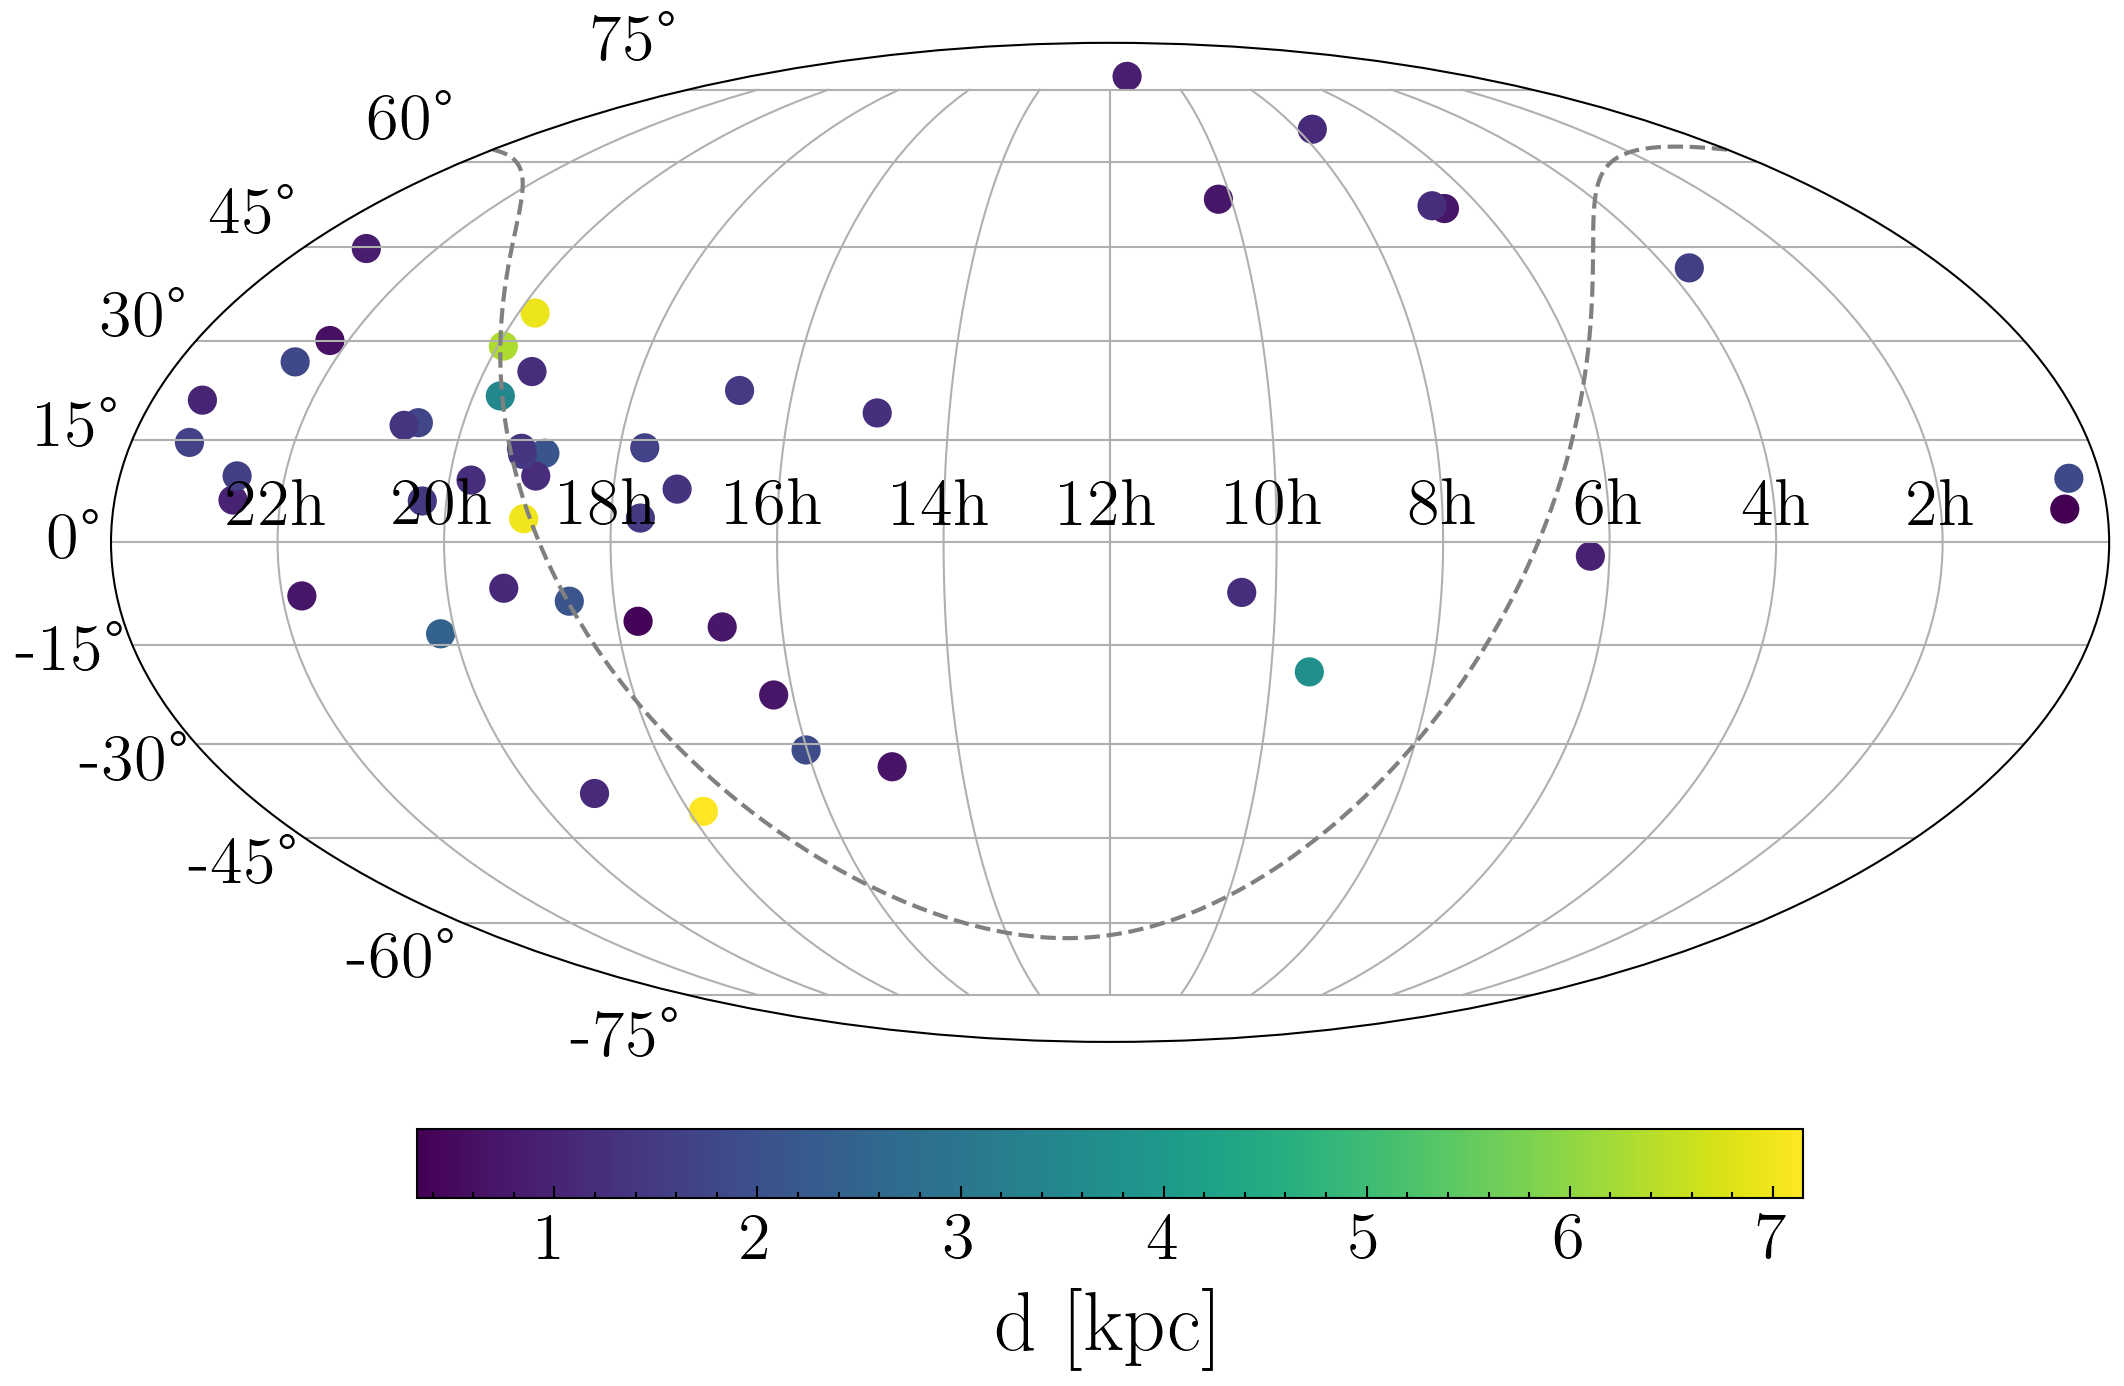
\includegraphics[width=\columnwidth]{images/pulsar_distribution}
	\caption{Spatial distribution \DIFaddbeginFL \DIFaddFL{in Galactic coordinates }\DIFaddendFL of 47 pulsars from the 12.5 year NANOGrav data release that make up the synthetic PTA used in this work. The pulsar distances relative to the observer are also indicated, with the majority of pulsars having a distance $\sim 1$ kpc. The grey dashed line denotes the Galactic plane.}
	\label{fig:pulsar_distrib}
\end{figure}
\DIFdelbegin \DIFdel{For this work we generate synthetic data that is astrophysically representative as follows. We first specify a set of pulsars to make up our artificial PTA . We take }\DIFdelend \DIFaddbegin \DIFadd{We consider, by way of illustration, a synthetic PTA composed of }\DIFaddend the 47 pulsars \DIFdelbegin \DIFdel{that make up }\DIFdelend \DIFaddbegin \DIFadd{in }\DIFaddend the 12.5 year NANOGrav \DIFdelbegin \DIFdel{PTA }\DIFdelend \DIFaddbegin \DIFadd{dataset }\DIFaddend \citep{2020ApJ...905L..34A}. The NANOGrav pulsars are chosen arbitrarily as being representative of a typical PTA\DIFdelbegin \DIFdel{and the method naturally extends }\DIFdelend \DIFaddbegin \DIFadd{; the analysis below extends unchanged }\DIFaddend to any other PTA. For each pulsar we \DIFdelbegin \DIFdel{obtain the sky location (which defines the vector $\boldsymbol{q}^{(n)}$), the distance, the barycentric rotation frequency (which we identify with $f_{\rm em}^{(n)} (t_1)$), and the time derivative of the the barycentric rotation frequency (which we identify with $\dot{f}_{\rm em}^{(n)} (t_1)$). The spatial distribution and the }\DIFdelend \DIFaddbegin \DIFadd{adopt the fiducial values for ${\boldsymbol{q}}^{(n)}$, $d^{(n)}$, $f_{\rm em}^{(n)}(t_1)$, and $\dot{f}_{\rm em}(t_1)$, with the latter two quantities evaluated at the Solar System barycenter. A table of fiducial values is presented in Appendix \ref{appendix_fiducial} for the sake of reproducibility. The sky positions and colour-coded }\DIFaddend distances of the pulsars \DIFdelbegin \DIFdel{used for this artificial PTA are shown }\DIFdelend \DIFaddbegin \DIFadd{are displayed }\DIFaddend in Figure \ref{fig:pulsar_distrib}. The \DIFdelbegin \DIFdel{data is }\DIFdelend \DIFaddbegin \DIFadd{pulsar parameters are }\DIFaddend acquired via the Australia Telescope National Facility (ATNF) pulsar catalogue \citep{Manchester2005} using the \texttt{psrqpy} package \citep{psrqpy}. The remaining \DIFdelbegin \DIFdel{unspecified }\DIFdelend \DIFaddbegin \DIFadd{static }\DIFaddend pulsar parameters are $\gamma^{(n)}$ and $\sigma^{(n)}$\DIFdelbegin \DIFdel{. We discussed in Section \ref{sec:psr_frequency} how the quantity $[\sigma^{(n)}]^2 /\gamma^{(n)} $ sets the amplitude of the characteristic }\DIFdelend \DIFaddbegin \DIFadd{, for which no direct measurements exist. The ratio $\sigma^{(n)} / [\gamma^{(n)}]^{1/2}$ sets the typical }\DIFaddend root mean square fluctuations in $f_p^{(n)}(t)$\DIFdelbegin \DIFdel{. Typically }\DIFdelend \DIFaddbegin \DIFadd{, as discussed in Section \ref{sec:psr_frequency} and }\DIFaddend the mean reversion timescale \DIFaddbegin \DIFadd{typically satisfies }\DIFaddend $[\gamma^{(n)}]^{-1} \gg T_{\rm obs}$ \DIFdelbegin \DIFdel{\mbox{%DIFAUXCMD
\citep{Vargas}}\hskip0pt%DIFAUXCMD
, whilst $[\sigma^{(n)}]^2$ varies between individual pulsars. For this work }\DIFdelend \DIFaddbegin \DIFadd{\mbox{%DIFAUXCMD
\citep{Price2012,Myers2021MNRAS.502.3113M,Meyers2021,Vargas}}\hskip0pt%DIFAUXCMD
. In this paper, for the sake of simplicity in the absence of independent measurements, }\DIFaddend we fix $\gamma^{(n)} = 10^{-13}$ s$^{-1}$ for all $n$. \DIFdelbegin \DIFdel{In }\DIFdelend \DIFaddbegin \DIFadd{We follow two complementary approaches in }\DIFaddend order to  set \DIFdelbegin \DIFdel{a physically reasonable value for $[\sigma^{(n)}]^2$ we use two complementary approaches}\DIFdelend \DIFaddbegin \DIFadd{physically reasonable values for $\sigma^{(n)}$}\DIFaddend . The first approach \DIFdelbegin \DIFdel{uses }\DIFdelend \DIFaddbegin \DIFadd{relies on }\DIFaddend the empirical timing noise model from \cite{Shannon2010ApJ...725.1607S} \DIFdelbegin \DIFdel{where }\DIFdelend \DIFaddbegin \DIFadd{which gives }\DIFaddend the standard deviation \DIFdelbegin \DIFdel{in the pulsar TOA is given by:
}\DIFdelend \DIFaddbegin \DIFadd{of the pulsar TOAs, $\sigma_{\rm TOA}^{(n)}$, empirically as
}\DIFaddend \begin{align}
	\ln \left(\frac{\sigma_{\rm TOA}^{(n)}}{\mu s} \right)\DIFdelbegin %DIFDELCMD < &%%%
\DIFdelend =\DIFaddbegin & \DIFaddend \ln \alpha_1 +  \alpha_2 \ln f_{\rm p}^{(n)} + \alpha_3 \ln \left(\frac{\dot{f}_{\rm p}^{(n)}}{10^{-15} \text{s}^{-2}} \right) \nonumber \\ 
	&+ \alpha_4 \ln \left( \DIFdelbegin \DIFdel{\frac{T}{ 1 \text{ year}} }\DIFdelend \DIFaddbegin \DIFadd{\frac{T_{\rm cad}}{ 1 \text{ year}} }\DIFaddend \right) \ , \label{eq:sigmap}
\end{align}
where \DIFdelbegin \DIFdel{$T$ is the length of the observation span }\DIFdelend \DIFaddbegin \DIFadd{$T_{\rm cad}$ is the cadence of the timing observations }\DIFaddend and for MSPs \DIFdelbegin \DIFdel{$\ln \alpha_1 \sim -20 $, $\alpha_2 \sim 1$, $\alpha_3 \sim 2$ and $\alpha_4 \sim 2.4$. }\DIFdelend \DIFaddbegin \DIFadd{the best fit parameters are $\ln \alpha_1 = -20 \pm 20$, $\alpha_2 = 1 \pm 2 $, $\alpha_3 = 2 \pm 1$, $\alpha_4 = 2.4 \pm 0.6$, for $\pm 2\sigma$ confidence limits. The uncertainties on these parameters are broad; for the purposes of generating astrophysically representative synthetic data we straightforwardly take the best fit parameter value. }\DIFaddend Throughout this work we assume that all pulsars are observed with a weekly cadence\DIFaddbegin \DIFadd{, $T_{\rm cad} = 1 \,{\rm week}$}\DIFaddend . In order to relate \DIFdelbegin \DIFdel{the empirical TOA noise model, }\DIFdelend Equation \eqref{eq:sigmap}, to \DIFdelbegin \DIFdel{our Ornstein-Uhlenbeck frequency model, }\DIFdelend \DIFaddbegin \DIFadd{$\sigma^{(n)}$ in }\DIFaddend Equation \eqref{eq:spinevol}, we \DIFdelbegin \DIFdel{set first $T = 1$ week in Equation \ref{eq:sigmap} to obtain an estimate of the TOA noise over a weekly time interval, i.e. the size of our numerical integration timestep. The frequency process noise parameter $\sigma^{(n)}$ can then be calculated for each pulsar where the standard deviation in the pulsar TOA can be related to the standard deviation in the pulsar frequency as 
}\DIFdelend \DIFaddbegin \DIFadd{equate $\sigma^{(n)}$ to the root mean square TOA noise accumulated over one week, obtaining
}\DIFaddend \begin{eqnarray}
	\sigma^{(n)} \DIFdelbegin \DIFdel{\sim }\DIFdelend \DIFaddbegin \DIFadd{\approx }\DIFaddend \sigma_{\rm TOA}^{(n)} \DIFdelbegin \DIFdel{\frac{f_{\rm p}^{(n)}}{T} }\DIFdelend \DIFaddbegin \DIFadd{f_{\rm p}^{(n)} }{\DIFadd{T_{\rm cad}}}\DIFadd{^{-1} }\DIFaddend \ . \label{eq:sigmap_f}
\end{eqnarray}
For \DIFdelbegin \DIFdel{our }\DIFdelend \DIFaddbegin \DIFadd{the }\DIFaddend synthetic NANOGrav PTA \DIFaddbegin \DIFadd{depicted in Figure \ref{fig:pulsar_distrib}}\DIFaddend , the median $\sigma^{(n)}$ calculated in this way is $\sigma^{(n)} = 4.28 \times 10^{-21} $ s\DIFdelbegin \DIFdel{. }\DIFdelend \DIFaddbegin \DIFadd{$^{-3/2}$, $\min [ \sigma^{(n)} ] = 1.3 \times 10^{-23}$s$^{-3/2}$ for PSR J0645+5158 and $\max [ \sigma^{(n)} ] = 2.0 \times 10^{-16}$ s$^{-3/2}$ for PSR J1939+2134 }\DIFaddend \newline 

As a \DIFdelbegin \DIFdel{sanity check, we can also calculate }\DIFdelend \DIFaddbegin \DIFadd{cross-check, we estimate }\DIFaddend $\sigma^{(n)}$ \DIFdelbegin \DIFdel{using a complementary numerical approach to the empirical best-fit model outlined above. We can directly solve the state equation }\DIFdelend \DIFaddbegin \DIFadd{by solving }\DIFaddend Equation \eqref{eq:spinevol} numerically using the \texttt{baboo} package \footnote{\url{https://github.com/meyers-academic/baboo}}\DIFdelbegin \DIFdel{so as to obtain }\DIFdelend \DIFaddbegin \DIFadd{, generating }\DIFaddend a synthetic phase solution,
\begin{eqnarray}
	\DIFdelbegin \DIFdel{\xi}\DIFdelend \DIFaddbegin \DIFadd{\varphi}\DIFaddend ^{(n)}(t) = \int_0^t dt' f^{(n)}_{\rm p}(t') \ ,
\end{eqnarray}
and \DIFdelbegin \DIFdel{generate TOAs and phase residuals. We calibrate the noise amplitude }\DIFdelend \DIFaddbegin \DIFadd{adjusting }\DIFaddend $\sigma^{(n)}$ \DIFaddbegin \DIFadd{iteratively }\DIFaddend to generate phase residuals \DIFdelbegin \DIFdel{that qualitatively }\DIFdelend \DIFaddbegin \DIFadd{which qualitatively (i.e.\ visually) }\DIFaddend resemble empirical phase residuals measured from real pulsars\DIFaddbegin \DIFadd{; see Section 2 in \mbox{%DIFAUXCMD
\cite{Vargas} }\hskip0pt%DIFAUXCMD
for a successful example of this approach}\DIFaddend . We obtain empirical phase residuals from the \DIFdelbegin \DIFdel{UTMOST pulsar timing program \mbox{%DIFAUXCMD
\citep{UTMOST} }\hskip0pt%DIFAUXCMD
from the  Molonglo Observatory Synthesis Telescope \mbox{%DIFAUXCMD
\citep{Bailes2017PASA...34...45B}}\hskip0pt%DIFAUXCMD
. For the purposes of validating the $\sigma^{(n)}$ inferred from Equation \eqref{eq:sigmap_f}, it is sufficient at this stage to simply compare the synthetic and real phase residuals visually. Whilst it would also be possible to e.g. define some quantitative loss function (e.g. mean-squared error) between the two solutions and solve the optimisation problem to infer $\sigma^{(n)}$, for our purposes this is excessive. It is satisfactory to simply qualitatively compare the two solutions as a useful sanity check. We emphasise that we are not overly concerned with calculating the maximally accurate }\DIFdelend \DIFaddbegin \DIFadd{NANOGrav 12.5 year wideband timing dataset \mbox{%DIFAUXCMD
\citep{pennucci_timothy_t_2020_4312887,nanogravwideband}}\hskip0pt%DIFAUXCMD
. A visual cross-check is sufficient for the purposes of this paper, where we seek broadly representative }\DIFaddend values for $\sigma^{(n)}$\DIFdelbegin \DIFdel{, but instead some reasonable values for constructing representative synthetic data . This approach of generating synthetic phase solutions and visually comparing with empirical solutions is also followed in \mbox{%DIFAUXCMD
\cite{Vargas}}\hskip0pt%DIFAUXCMD
}\DIFdelend \DIFaddbegin \DIFadd{. In an analysis involving real PTA data, $\sigma^{(n)}$ would be estimated from the data jointly with the other static parameters in ${\boldsymbol{\theta}}$}\DIFaddend . In Figure \ref{fig:qualitative_compare} we compare the synthetic and empirical residuals for \DIFdelbegin \DIFdel{the NANOGrav pulsar J0030}\DIFdelend \DIFaddbegin \DIFadd{PSR J1939}\DIFaddend +\DIFdelbegin \DIFdel{0451. We can }\DIFdelend \DIFaddbegin \DIFadd{2134, one of the 47 NANOGrav pulsars plotted in Figure \ref{fig:pulsar_distrib}. We }\DIFaddend see that the synthetic and empirical residuals are qualitatively similar\DIFdelbegin \DIFdel{, and comparable behaviour is observed for other pulsars in our array}\DIFdelend \DIFaddbegin \DIFadd{. For this pulsar the synthetic residuals were generated using $\sigma^{(n)} = 10^{-27}$ s$^{-3/2}$ which is $\ll$ than the value inferred from the noise model of Equations \eqref{eq:sigmap} and \eqref{eq:sigmap_f}, using the best fit parameters, $\sigma^{(n)} = 2.0 \times 10^{-16}$ s$^{-3/2}$. This highlights how given the large uncertainties on the parameters of Equation \eqref{eq:sigmap} using the best fit values may be less appropriate for certain pulsars. This discrepancy between the two estimates of $\sigma^{(n)}$ is particular to PSR J1939+2134; for all other pulsars we find the two estimates of $\sigma^{(n)}$ are comparable to within a few orders of magnitude}\DIFaddend .
\begin{figure}
	\DIFdelbeginFL %DIFDELCMD < 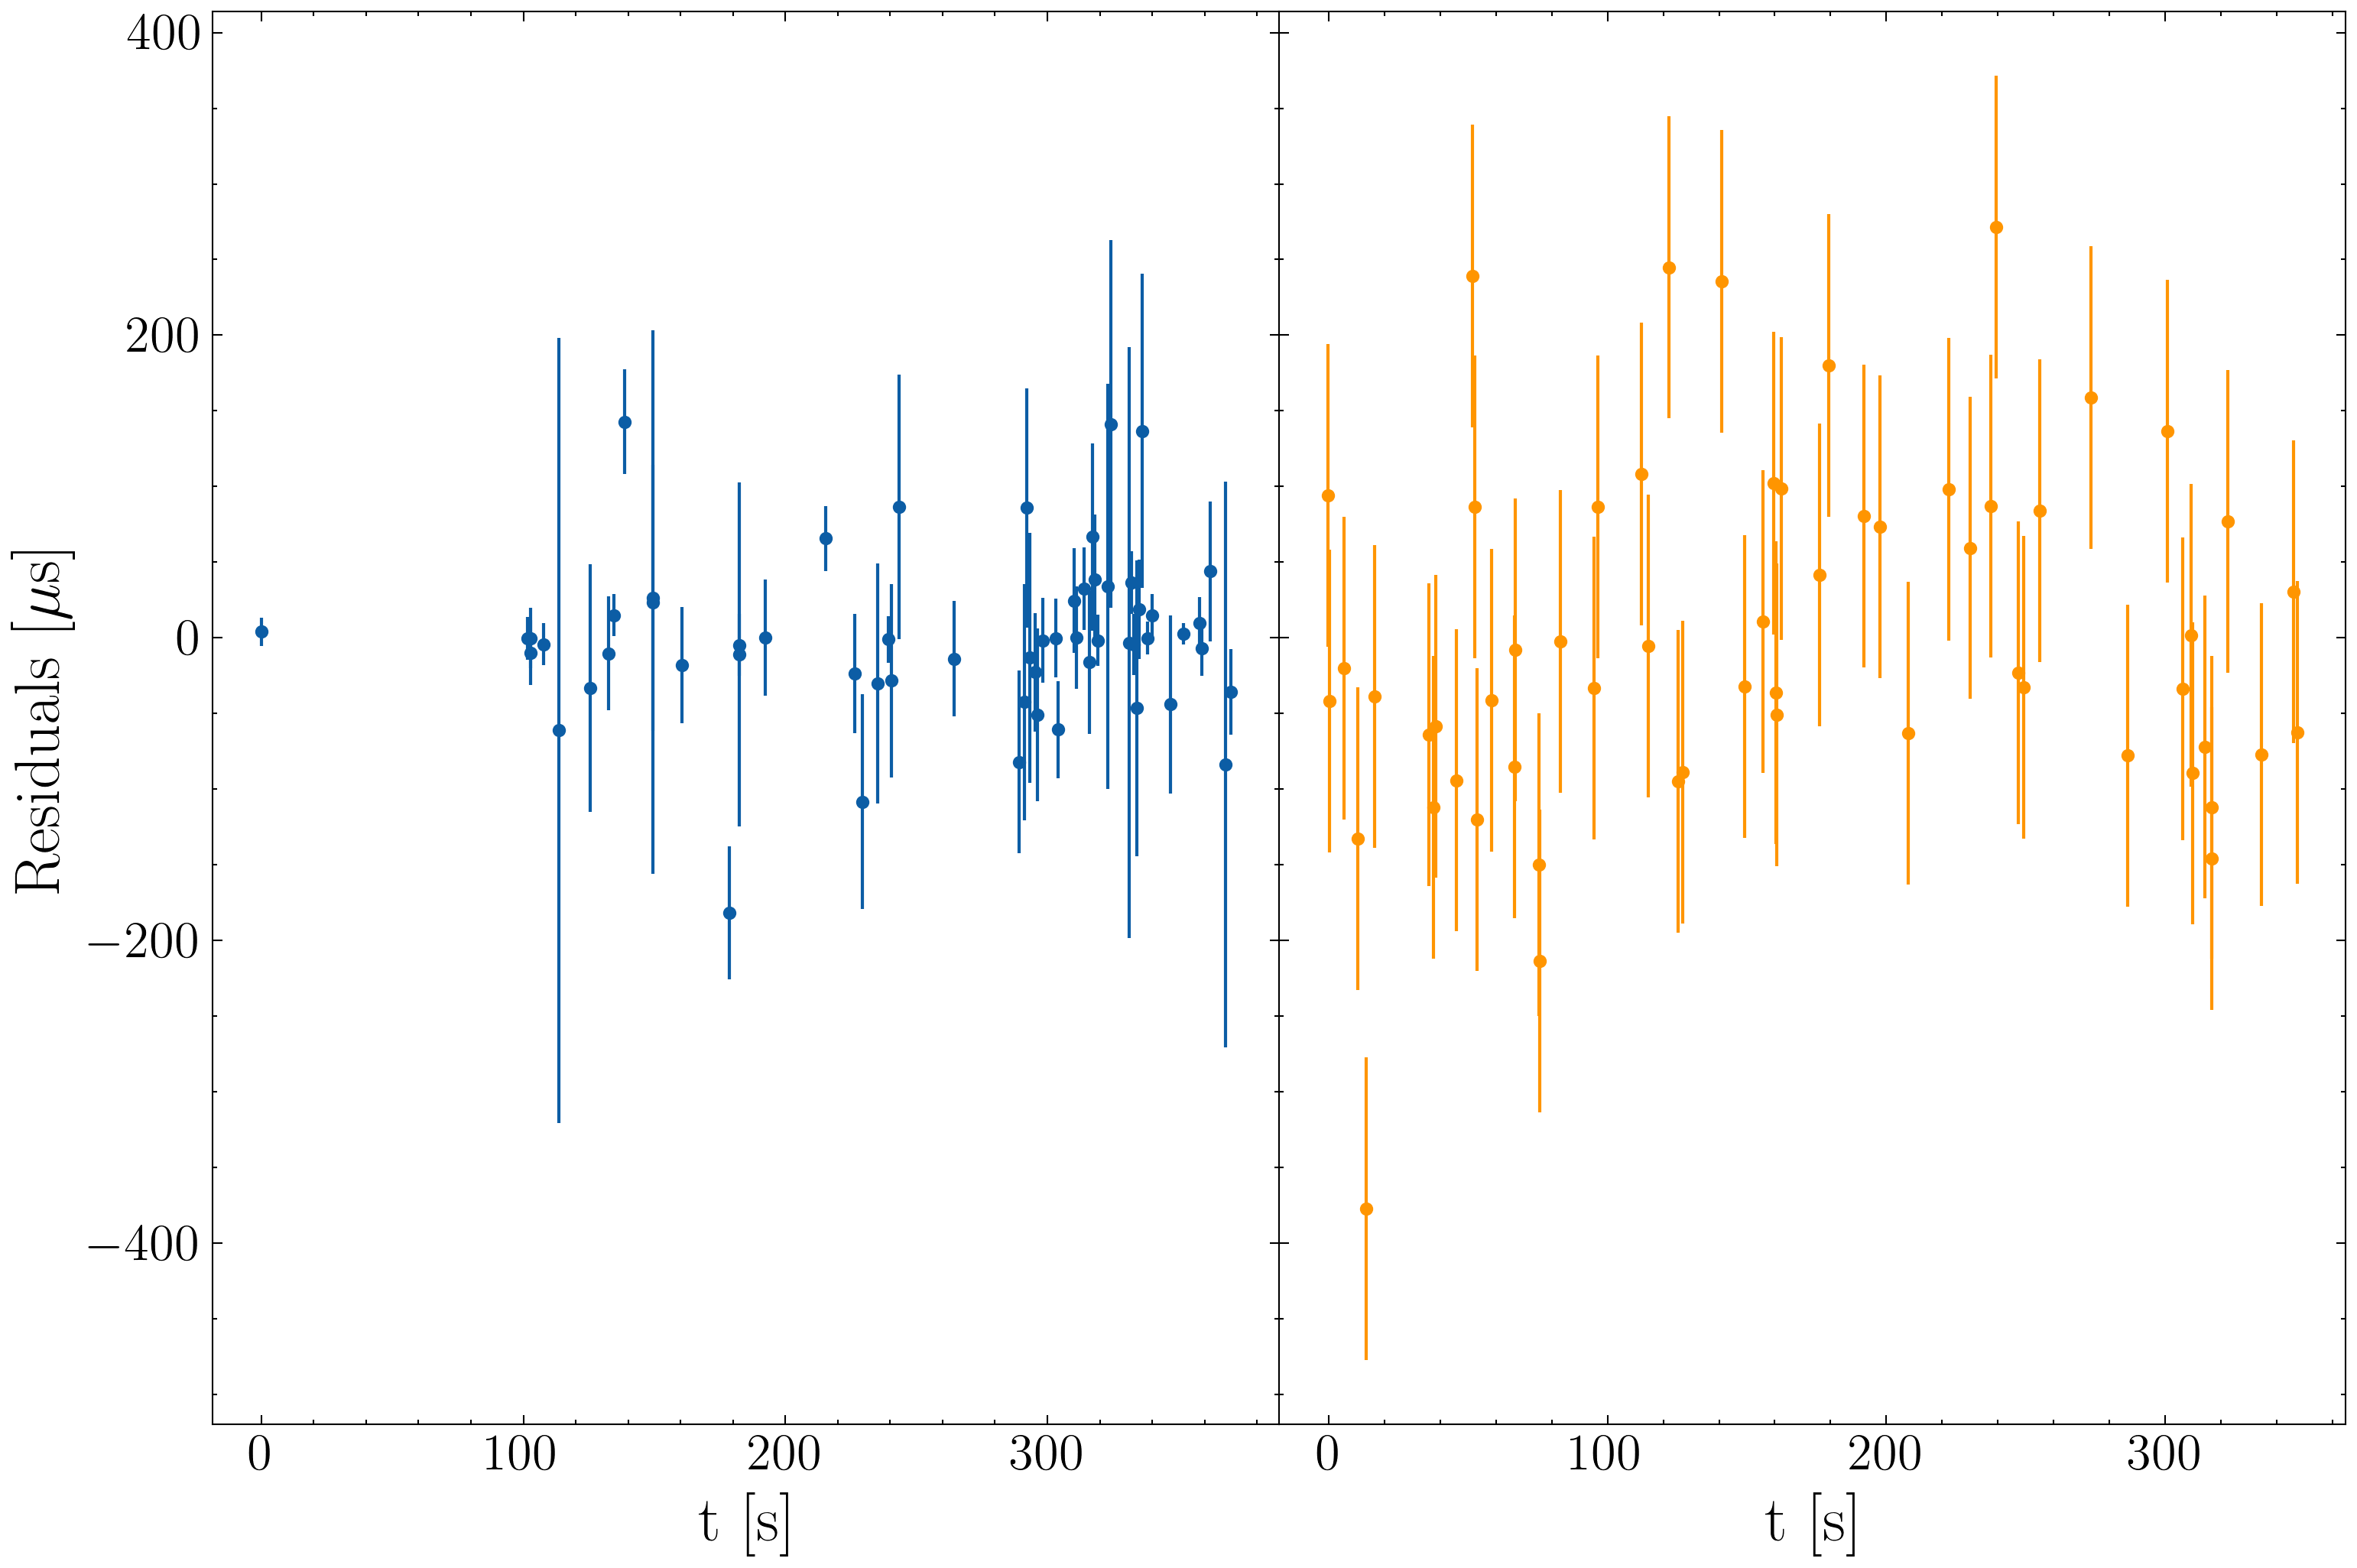
\includegraphics[width=\columnwidth]{images/example_residuals_plot}
%DIFDELCMD < 	%%%
\DIFdelendFL \DIFaddbeginFL 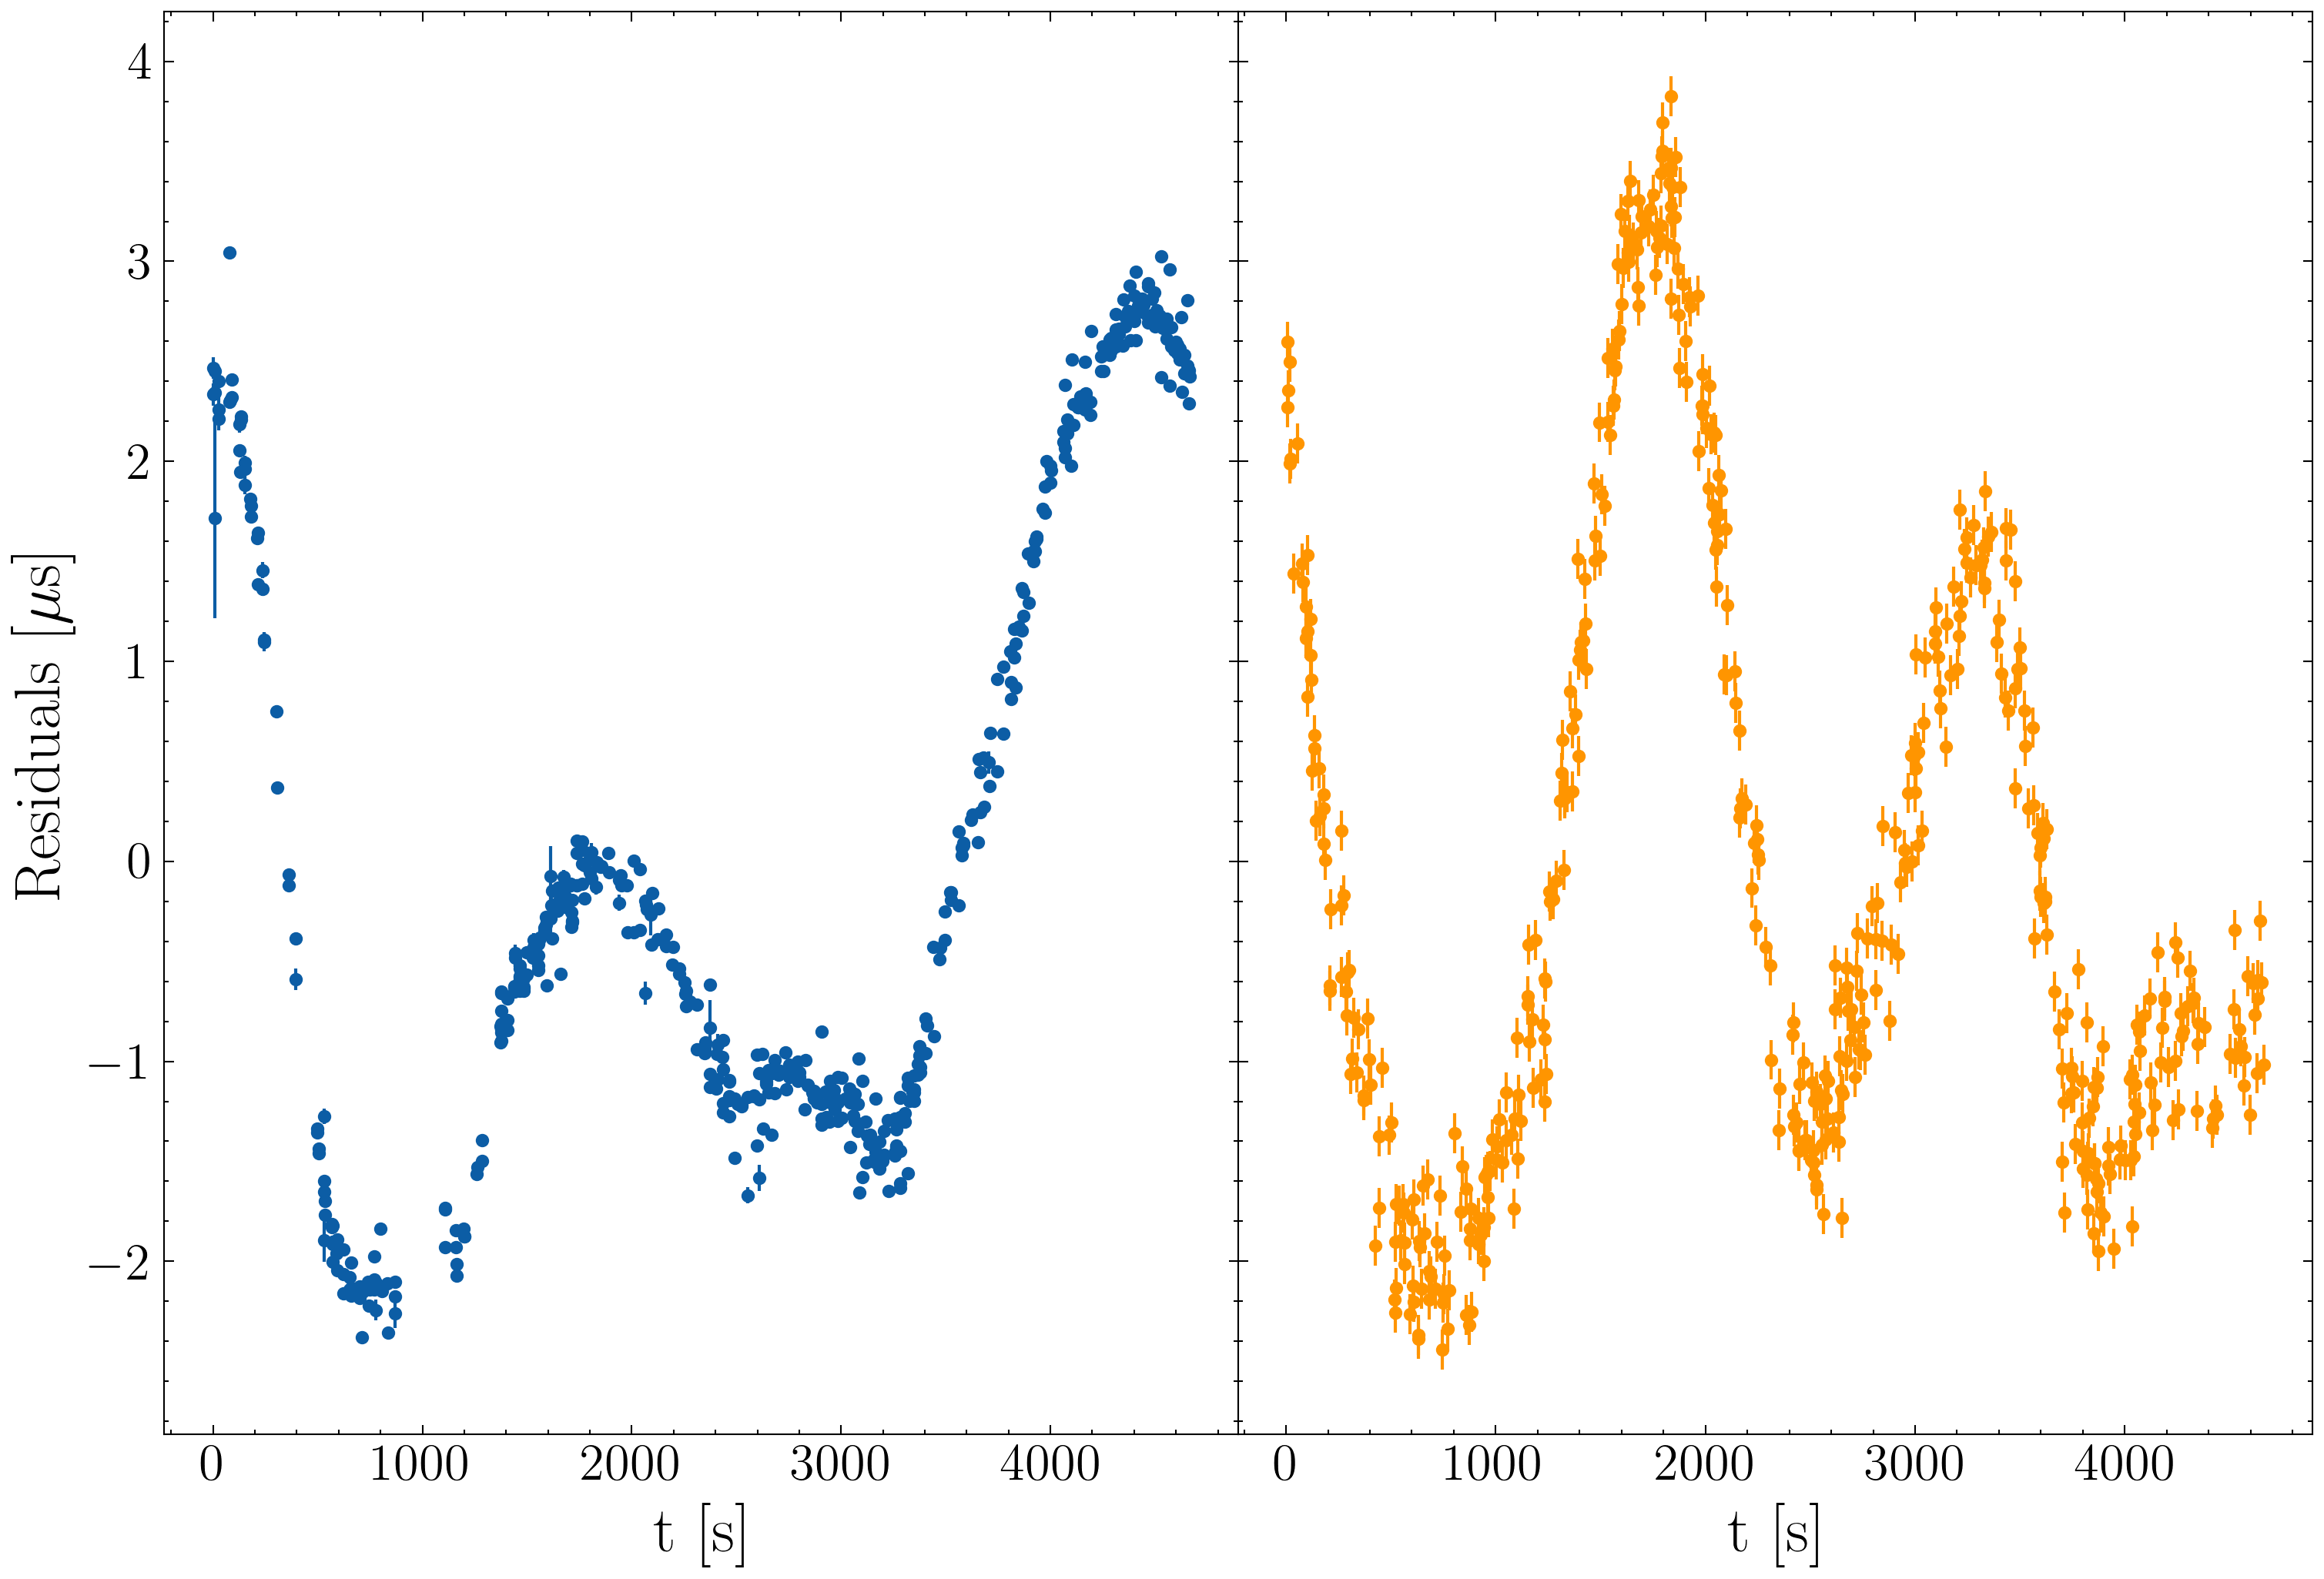
\includegraphics[width=\columnwidth]{images/example_residuals_plot2}
	\DIFaddendFL \caption{Actual (left \DIFdelbeginFL \DIFdelFL{panels}\DIFdelendFL \DIFaddbeginFL \DIFaddFL{panel, blue points}\DIFaddendFL ) and synthetic (right \DIFdelbeginFL \DIFdelFL{panels}\DIFdelendFL \DIFaddbeginFL \DIFaddFL{panel, orange points}\DIFaddendFL ) phase residuals for NANOGrav millisecond pulsar \DIFdelbeginFL \DIFdelFL{J0030}\DIFdelendFL \DIFaddbeginFL \DIFaddFL{PSR J1939}\DIFaddendFL +\DIFdelbeginFL \DIFdelFL{0451. }\DIFdelendFL \DIFaddbeginFL \DIFaddFL{2134. }\DIFaddendFL The actual residuals are \DIFdelbeginFL \DIFdelFL{obtained via UTMOST pulsar }\DIFdelendFL \DIFaddbeginFL \DIFaddFL{sourced from the NANOGrav 12.5 year wideband }\DIFaddendFL timing \DIFdelbeginFL \DIFdelFL{program \mbox{%DIFAUXCMD
\citep{UTMOST}}\hskip0pt%DIFAUXCMD
}\DIFdelendFL \DIFaddbeginFL \DIFaddFL{dataset \mbox{%DIFAUXCMD
\citep{pennucci_timothy_t_2020_4312887,nanogravwideband}}\hskip0pt%DIFAUXCMD
}\DIFaddendFL . The synthetic residuals are generated by numerically solving Equation \eqref{eq:spinevol} with $\gamma^{(n)} = 10^{-13}$ and \DIFdelbeginFL \DIFdelFL{$\sigma^{(n)}$ inferred from Equations \eqref{eq:sigmap} }\DIFdelendFL \DIFaddbeginFL \DIFaddFL{$\sigma^{(n)} = 2\times 10^{-27}$ s$^{-3/2}$. The error bars indicate the uncertainty in the phase residuals }\DIFaddendFL and \DIFdelbeginFL \DIFdelFL{\eqref{eq:sigmap_f}}\DIFdelendFL \DIFaddbeginFL \DIFaddFL{are generated by propagating the uncertainty in the TOAs through }{\sc \DIFaddFL{tempo2}}\DIFaddendFL . \DIFdelbeginFL \DIFdelFL{For all pulsars }\DIFdelendFL \DIFaddbeginFL \DIFaddFL{We set }\DIFaddendFL the \DIFdelbeginFL \DIFdelFL{two solutions }\DIFdelendFL \DIFaddbeginFL \DIFaddFL{TOA uncertainty to be a constant $0.1 \mu$s. The blue and orange residuals }\DIFaddendFL are qualitatively similar \DIFdelbeginFL \DIFdelFL{, with comparable magnitudes }\DIFdelendFL \DIFaddbeginFL \DIFaddFL{by inspection. Similar results are obtained for the other 46 pulsars }\DIFaddendFL in the \DIFdelbeginFL \DIFdelFL{residuals}\DIFdelendFL \DIFaddbeginFL \DIFaddFL{synthetic PTA in Section \ref{sec:synt_pta} by tuning the value of $\sigma^{(n)}$}\DIFaddendFL .}
	\label{fig:qualitative_compare}
\end{figure}
\DIFdelbegin \subsubsection{\DIFdel{Synthetic data generation}}
%DIFAUXCMD
\addtocounter{subsubsection}{-1}%DIFAUXCMD
\DIFdelend \DIFaddbegin \subsection{\DIFadd{Generating a synthetic sequence of pulse frequencies}}\label{sec:gendata}
\DIFaddend We generate $N$ synthetic noisy \DIFdelbegin \DIFdel{timeseries}\DIFdelend \DIFaddbegin \DIFadd{time series of the measured pulse frequency $f_{\rm m}^{(n)}(t)$}\DIFaddend , one for each pulsar \DIFaddbegin \DIFadd{$1\leq n \leq N$}\DIFaddend , as follows:
\DIFdelbegin %DIFDELCMD < 

%DIFDELCMD < \begin{enumerate}
%DIFDELCMD < 	%%%
\DIFdelend \DIFaddbegin \begin{enumerate}[leftmargin=2em]
	\DIFaddend \item Integrate \DIFdelbegin \DIFdel{the state equations, }\DIFdelend Equations \eqref{eq:spinevol}--\eqref{eq:xieqn} numerically for the synthetic PTA described in Section \ref{sec:synt_pta}\DIFaddbegin \DIFadd{, to obtain random realizations of $f_{\rm p}^{(n)}(t)$ for $1\leq n \leq N$}\DIFaddend .
	\item Map from \DIFdelbegin \DIFdel{state space to measurement space via the measurement equation, Equation \eqref{eq:measurement} }%DIFDELCMD < \item %%%
\item%DIFAUXCMD
\DIFdel{Add zero-mean Gaussian measurement noise to each timeseries, i.e. $f_{\rm m} ^{(n)} + \varepsilon^{(n)}$ where 	$\langle \varepsilon(t) \varepsilon(t') \rangle = \sigma_{\rm m}^2 \delta(t - t')$ for measurement noise covariance $\sigma_{\rm m}^2$.
}\DIFdelend \DIFaddbegin \DIFadd{$f_{\rm p}^{(n)}(t)$ to $f_{\rm m}^{(n)}(t)$ via Equations \eqref{eq:measurement} and \eqref{eq:g_func}
}\DIFaddend \end{enumerate}
Equations \eqref{eq:spinevol}--\eqref{eq:xieqn} are solved by a Runge-Kutta It$\hat{\text{o}}$ integrator implemented in the \texttt{sdeint} python package \footnote{\url{https://github.com/mattja/sdeint}}. The static pulsar parameters  $\boldsymbol{\theta}_{\rm psr}$ are completely specified \DIFdelbegin \DIFdel{by our construction of }\DIFdelend \DIFaddbegin \DIFadd{for }\DIFaddend the synthetic PTA outlined in Section \eqref{sec:synt_pta}. For this work we consider all pulsars to be observed for $T_{\rm obs} =10$ years, uniformly sampled with a weekly cadence. The measurement noise \DIFaddbegin \DIFadd{covariance as defined in Equation \eqref{eq:vareps} }\DIFaddend can be approximately related to the uncertainty in the pulse TOA, $\sigma_{\rm TOA}$, as
\begin{equation}
	\sigma_{\rm m} \DIFdelbegin \DIFdel{\sim }\DIFdelend \DIFaddbegin \DIFadd{\approx }\DIFaddend f_{\rm p}^{(n)} \DIFdelbegin \DIFdel{\frac{\sigma_{\rm TOA}}{\text{T}} }\DIFdelend \DIFaddbegin \DIFadd{\sigma_{\rm TOA} \ {T_{\rm cad}}^{-1} }\DIFaddend \ . \DIFaddbegin \label{eq:sigma_m_eqn}
\DIFaddend \end{equation}
\DIFaddbegin \DIFadd{Although Equations \eqref{eq:sigmap_f} and \eqref{eq:sigma_m_eqn} superficially resemble one another, they are distinct; Equation \eqref{eq:sigmap_f} deals with the timing noise intrinsic to the pulsar due to rotational irregularities, whereas Equation \eqref{eq:sigma_m_eqn} handles the detector measurement noise. }\DIFaddend For a millisecond pulsar with $f_{\rm p}^{(n)} \sim 100$ Hz observed with a weekly cadence and $\sigma_{\rm TOA} \sim 1 \mu$s \DIFdelbegin \DIFdel{this gives }\DIFdelend \DIFaddbegin \DIFadd{Equation \eqref{eq:sigma_m_eqn} implies }\DIFaddend $\sigma_{\rm m} \sim 10^{-10}$ \DIFdelbegin \DIFdel{, whilst the very best }\DIFdelend \DIFaddbegin \DIFadd{Hz. The most accurately timed }\DIFaddend pulsars might have $\sigma_{\rm TOA} \sim 10 $ ns or $\sigma_{\rm m} \sim 10^{-12}$ \DIFaddbegin \DIFadd{Hz}\DIFaddend . Throughout this \DIFdelbegin \DIFdel{work }\DIFdelend \DIFaddbegin \DIFadd{paper }\DIFaddend we fix $\sigma_{\rm m} = 10^{-11}$ Hz and take it \DIFdelbegin \DIFdel{to be }\DIFdelend \DIFaddbegin \DIFadd{as }\DIFaddend known \textit{a priori} rather than a parameter to be inferred. Note that whilst $\sigma_{\rm m}$ is the same for every pulsar, $f_{\rm m} ^{(n)}$ is modified by a different realisation of the measurement noise \DIFdelbegin \DIFdel{; whilst for our construction every pulsaris sampled at the same time and so would experience the same realisation of the noise, in actual pulsar astronomy different pulsars will be sampled at different times by different radio interferometers and so subject to different noise realisations}\DIFdelend \DIFaddbegin \DIFadd{for each pulsar}\DIFaddend . \newline 

\DIFdelbegin \DIFdel{In practice, in order to avoid numerical precision issues that arise }\DIFdelend \DIFaddbegin \DIFadd{Finite precision arithmetic leads to numerical errors }\DIFaddend when solving Equations \eqref{eq:spinevol}--\eqref{eq:xieqn} \DIFdelbegin \DIFdel{$\left ( \text{since } \sigma^{(n)} \ll f_{\rm p}^{(n)} \right)$ we first ``heterodyne" our state by subtracting }\DIFdelend \DIFaddbegin \DIFadd{$ \text{in  the regime } \sigma^{(n)} \Delta W_t \ll f_{\rm p}^{(n)}$ relevant to PTAs, where $\Delta W_t$ labels an increment of Brownian motion (see Appendix \ref{sec:kalman}). To fix the problem, we subtract }\DIFaddend the deterministic frequency evolution \DIFaddbegin \DIFadd{and track the new variable}\DIFaddend , equivalent to a change of variables:
\begin{equation}
	f_{\rm p}\DIFdelbegin \DIFdel{^{\prime (n)} }\DIFdelend \DIFaddbegin \DIFadd{^{* (n)} }\DIFaddend = f_{\rm p}^{(n)} - f_{\rm em}^{(n)} \ .
\end{equation}  
We similarly \DIFdelbegin \DIFdel{heterodyne }\DIFdelend \DIFaddbegin \DIFadd{modify }\DIFaddend the measurement variable \DIFaddbegin \DIFadd{to be
}\DIFaddend \begin{equation}
	f_{\rm m}\DIFdelbegin \DIFdel{^{\prime (n)} }\DIFdelend \DIFaddbegin \DIFadd{^{* (n)} }\DIFaddend = f_{\rm m}^{(n)} - f_{\rm em}\DIFdelbegin \DIFdel{^{*(n)} }\DIFdelend \DIFaddbegin \DIFadd{^{\diamond (n)} }\DIFaddend \ ,
\end{equation}
where \DIFdelbegin \DIFdel{$ f_{\rm em}^{*(n)}$ }\DIFdelend \DIFaddbegin \DIFadd{$ f_{\rm em}^{\diamond (n)}$ }\DIFaddend is a guess of the deterministic spin-down based on the pulsar ephemeris \DIFaddbegin \DIFadd{which is measured to high accuracy in practice by }{\sc \DIFadd{tempo2}}\DIFaddend . For synthetic data we can set \DIFdelbegin \DIFdel{$ f_{\rm em}^{*(n)} = f_{\rm em}^{(n)}$ }\DIFdelend \DIFaddbegin \DIFadd{$ f_{\rm em}^{\diamond (n)} = f_{\rm em}^{(n)}$ without loss of generality, }\DIFaddend but this is \DIFdelbegin \DIFdel{not true generally for real-world observationssince }\DIFdelend \DIFaddbegin \DIFadd{impossible generally for astronomical observations, because }\DIFaddend the spin-down ephemeris is only known approximately. \DIFdelbegin \DIFdel{The measurement equation Equation \eqref{eq:measurement} that relates the state and measurement variables }\DIFdelend \DIFaddbegin \DIFadd{Equation \eqref{eq:measurement} }\DIFaddend is then updated \DIFdelbegin \DIFdel{as 
}\DIFdelend \DIFaddbegin \DIFadd{to read 
}\DIFaddend \begin{equation}
	f_{\rm m}\DIFdelbegin \DIFdel{^{\prime (n)}}\DIFdelend \DIFaddbegin \DIFadd{^{* (n)}}\DIFaddend (t) = f_{\rm p}\DIFdelbegin \DIFdel{^{\prime (n)}}\DIFdelend \DIFaddbegin \DIFadd{^{* (n)}}\DIFaddend (t-d) g^{(n)}(t) -  f_{\rm em}^{(n)}(t-d)\left[ 1-g^{(n)}(t)\right] \ .
	\label{eq:measurement_cov}
\end{equation}
We emphasise that this change of variables is \DIFdelbegin \DIFdel{simply a convenient scaling to bring our }\DIFdelend \DIFaddbegin \DIFadd{a convenient device to bring the }\DIFaddend numerical values into a reasonable dynamic range without having to use \DIFdelbegin \DIFdel{extended numerical }\DIFdelend \DIFaddbegin \DIFadd{excessively long }\DIFaddend floating point formats (e.g. long double, quadruple). It does not remove any degrees of freedom \DIFdelbegin \DIFdel{of the formulation}\DIFdelend \DIFaddbegin \DIFadd{nor does it involve an approximation}\DIFaddend . In particular \DIFdelbegin \DIFdel{both }\DIFdelend $f_{\rm em}^{(n)}(t_1)$
and $\dot{f}_{\rm em}^{(n)}(t_1)$ remain \DIFdelbegin \DIFdel{static parameters of the model, but now }\DIFdelend \DIFaddbegin \DIFadd{as static parameters but }\DIFaddend appear in the measurement equation \DIFaddbegin \DIFadd{\eqref{eq:measurement_cov} }\DIFaddend rather than the \DIFdelbegin \DIFdel{state equation}\DIFdelend \DIFaddbegin \DIFadd{dynamical state equations, Equations \ref{eq:spinevol}--\eqref{eq:xieqn}}\DIFaddend .


\DIFdelbegin \subsection{\DIFdel{Representative example}}%DIFAUXCMD
\addtocounter{subsection}{-1}%DIFAUXCMD
\DIFdelend \DIFaddbegin \section{\DIFadd{Representative example: single SMBHB source}}\DIFaddend \label{sec:rep_example}
\DIFdelbegin \DIFdel{We initially characterise our method with a single example of }\DIFdelend \DIFaddbegin \DIFadd{In this Section we apply the analysis scheme of Section \ref{sec:detect} and the validation procedure of Section \ref{sec:testing} to }\DIFaddend a PTA which is perturbed by a GW from an individual quasi-monochromatic SMBHB source. \DIFaddbegin \DIFadd{We remind the reader that the analysis in this paper targets a single SMBHB source. The analysis of a stochastic background composed of the superposition of multiple sources is more challenging and is postponed to a forthcoming paper. In Section \ref{sec:priors} we outline the priors chosen on $\boldsymbol{\theta}$. In Section \ref{sec:parameter_estim} we apply the workflow of Section \ref{sec:methodsummary} to estimate $\boldsymbol{\theta}$, for a single realisation of the pulsar process noise and the measurement noise. We go on in Section \ref{sec:multiple_noise} to extend this parameter estimation procedure to multiple realisations of the noise processes. In Section \ref{sec:detection} we calculate the the detectability of the source as a function of $h_0$. }\newline


\DIFaddend The static GW source parameters $\boldsymbol{\theta}_{\rm gw}$ used for this injection are selected to be astrophysically reasonable and representative. The injected $\boldsymbol{\theta}_{\rm gw}$ are summarised in the ``Injected Values" column of Table \ref{tab:parameters_and_priors}. The static pulsar parameters $\boldsymbol{\theta}_{\rm psr}$ are as described in Section \ref{sec:synt_pta} and are also shown in Table \ref{tab:parameters_and_priors}. 

\DIFdelbegin \subsubsection{\DIFdel{Prior distributions}}%DIFAUXCMD
\addtocounter{subsubsection}{-1}%DIFAUXCMD
\DIFdelend \DIFaddbegin \subsection{\DIFadd{Prior distributions}}\DIFaddend \label{sec:priors}
For the Bayesian methods used in this work, one must select reasonable priors, $\pi(\boldsymbol{\theta})$, for the complete set complete of static parameters. For $\pi(\boldsymbol{\theta}_{\rm gw})$ we choose standard non-informative priors \citep[e.g.][]{Bhagwat2021} as summarised in Table \ref{tab:parameters_and_priors}. The choice of $\pi(\boldsymbol{\theta}_{\rm psr})$ requires some additional discussion. \newline 


The parameters which govern the deterministic evolution of the pulsar spin frequency, $f_{\rm em}^{(n)} (t_1)$ and $\dot{f}_{\rm em}^{(n)} (t_1)$ are well-determined by existing radio timing observations. We can identify $f_{\rm em}^{(n)} (t_1)$ with the pulsar barycentric rotation frequency and $\dot{f}_{\rm em}^{(n)} (t_1)$ with the time derivative of barycentric rotation frequency quoted by pulsar observation catalogues. For the 12.5 year NANOGrav pulsars the median error in  the barycentric rotation frequency is $\sim 7 \times 10^{-13}$ Hz, and in the time derivative of barycentric rotation frequency is $\sim 1.8 \times 10^{-20}$ s $^{-2}$. Whilst it is then clear that $f_{\rm em}^{(n)} (t_1)$, $\dot{f}_{\rm em}^{(n)} (t_1)$ are typically measured with very high precisions, for this work we adopt a broader uniform prior, $\pm 10^3 \epsilon^{(n)}_{a}$ either side of the true value, where $\epsilon^{(n)}_{a}$ is the error for that pulsar quoted in the ATNF catalogue and the subscript $a = \{ f, \dot{f} \}$ identifies the error as being in $f_{\rm em}^{(n)} (t_1)$, or $\dot{f}_{\rm em}^{(n)} (t_1)$ respectively. In this way we can test how well our method performs without requiring exceptionally precise and accurate measurements of the pulsar parameters to be made \textit{a priori}. Instead we consider the pulsar parameters similarly to the GW source parameters and estimate them optimally within a consistent framework. Adopting looser priors in this way allows us to subject our method to a more stringent test and confirm that we still accurately estimate GW parameters without highly accurate and precise initial estimates of $f_{\rm em}^{(n)} (t_1)$ and $\dot{f}_{\rm em}^{(n)} (t_1)$. \newline 


The pulsar distances $d^{(n)}$ are typically not as well constrained as $f_{\rm em}^{(n)} (t_1)$ and $\dot{f}_{\rm em}^{(n)} (t_1)$, with uncertainties typically on the order of $\sim 10 \%$ \citep{Arzoumanian2018ApJS..235...37A,Yao2017}. However for this work, whilst the pulsar distance is used when generating synthetic data, as is discussed in Section \ref{sec:parameter_estim} the pulsar distance is not used for our inference model and so we do not need to set a prior on $d^{(n)}$. Similarly we do not set a prior on $\gamma^{(n)}$; since $[\gamma^{(n)}]^{-1} \gg T_{\rm obs}$ this means that $\gamma^{(n)}$ is effectively ``unobservable" over the decadal timescales that we are interested in. That is, for $T_{\rm obs}$ =10 years the solution of Equation \eqref{eq:spinevol} is effectively independent of the choice of $\gamma^{(n)}$ as long as the condition $[\gamma^{(n)}]^{-1} \gg T_{\rm obs}$ is satisfied. It is therefore sufficient to consider $\gamma^{(n)}$ to be known \textit{a priori} and set it at its true injected value. We briefly explored setting an uninformative prior on $\gamma^{(n)}$ over e.g. LogUniform($10^{-15}, 10^{-10}$) s$^{-1}$ as well as setting $\gamma^{(n)}$ at some fixed value away from the true injected value (e.g. set $\gamma^{(n)} = 10^{-14} \text{s}^{-1}$ rather than $10^{-13} \text{s}^{-1}$) but the results are unchanged. Regarding $\sigma^{(n)}$, the majority of pulsars in our synthetic PTA have \DIFdelbegin \DIFdel{$\sigma^{(n)} \sim 10^{-20} - 10^{-22} \text{ s}^{-5/2}$ }\DIFdelend \DIFaddbegin \DIFadd{$\sigma^{(n)} \sim 10^{-20} - 10^{-22} \text{ s}^{-3/2}$ }\DIFaddend as calculated from Equations \eqref{eq:sigmap} and \eqref{eq:sigmap_f}. For these pulsars we set an uninformative broad prior of LogUniform($10^{-23}, 10^{-19}$ \DIFdelbegin \DIFdel{$\text{s}^{-5/2}$}\DIFdelend \DIFaddbegin \DIFadd{$\text{s}^{-3/2}$}\DIFaddend ). The single exception is PSR J1939+2134 which has a particularly large $\dot{f}_{\rm em}^{(n)} (t_1)$ compared to the other pulsars in the array and so \DIFdelbegin \DIFdel{$\sigma \sim 10^{-16} \text{s}^{-5/2}$}\DIFdelend \DIFaddbegin \DIFadd{$\sigma \sim 10^{-16} \text{s}^{-3/2}$}\DIFaddend . For our artificial dataset we set \DIFdelbegin \DIFdel{$\sigma = 10^{-21} \text{s}^{-5/2}$ }\DIFdelend \DIFaddbegin \DIFadd{$\sigma = 10^{-21} \text{s}^{-3/2}$ }\DIFaddend for this pulsar in order to bring the process noise for all pulsars into a consistent range that can be described by a single constrained prior. \newline 


Since we are not setting priors on $\gamma^{(n)}$ or $d^{(n)}$ this reduces the dimensionality of the parameter space to $7 + 3N$. We use the notation $\boldsymbol{\theta}_{\rm psr, reduced}$ to refer to the reduced parameter space, c.f. Equation \ref{eq:psrparams}. Explicitly, 
\begin{equation}
	\boldsymbol{\theta}_{\rm psr, reduced} = \left \{ f_{\rm em}^{(n)}(t_1),\dot{f}_{\rm em}^{(n)}(t_1),\sigma^{(n)}\right\}_{1\leq n \leq N} \ .
\end{equation}
All the injected static parameters and their corresponding priors for this representative example are summarised in Table \ref{tab:parameters_and_priors}.
\begin{table*}
	\centering
%	\resizebox{\textwidth}{!}{%
%	\renewcommand{\arraystretch}{1.0} % Default value: 1
	\begin{tabular}{lccll}
		\toprule
		&Parameter & Injected Values & Units & Prior  \\
		\hline
		\multirow{7}{2mm}{$\boldsymbol{\theta}_{\rm gw}$} & $\Omega$       & $5 \times 10^{-7}$ & Hz & LogUniform($10^{-9}$, $10^{-5}$) \\
	  & $\alpha$          & $1.0$  & radians & Uniform($0, 2 \pi $)\\
	  & $\delta$              & $1.0$  & radians & Uniform($-\pi/2, \pi/2$) \\
	  & $\psi$              & $2.50$ & radians & Uniform($0, 2 \pi $) \\
	  & $\Phi_0$          & $0.20$ & radians & Uniform($0, 2 \pi $) \\
	  & $h_0$            & $5 \times 10^{-15}$ & - & LogUniform($10^{-15}$, $10^{-9}$) \\
	  & $\iota$             & $1.0$ & radians & Uniform($0, \pi$) \\ 
		\hline
		\multirow{5}{2mm}{$\boldsymbol{\theta}_{\rm psr}$} & $f_{\rm em}^{(n)} (t_1)$       & $f_{\rm ATNF}^{(n)}$ & Hz & Uniform$\left( f_{\rm ATNF}^{(n)} - 10^3 \epsilon^{(n)}_{f}, f_{\rm ATNF}^{(n)} + 10^3 \epsilon^{(n)}_{f} \right)$ \\
		& $\dot{f}_{\rm em}^{(n)} (t_1)$       & $\dot{f}_{\rm ATNF}^{(n)}$ & s$^{-2}$ & Uniform$\left( \dot{f}_{\rm ATNF}^{(n)} - 10^3 \epsilon^{(n)}_{\dot{f}}, \dot{f}_{\rm ATNF}^{(n)} + 10^3 \epsilon^{(n)}_{\dot{f}} \right)$ \\
		&  $d^{(n)}$       &$d_{\rm ATNF}^{(n)}$  & m & - \\
		& $\sigma^{(n)}$              & $\sigma_{\rm sc}^{(n)}$ & \DIFdelbeginFL \DIFdelFL{$s^{-5/2}$ }\DIFdelendFL \DIFaddbeginFL \DIFaddFL{$s^{-3/2}$ }\DIFaddendFL & LogUniform($10^{-23}, 10^{-19}$) \\
		& $\gamma^{(n)}$              & $10^{-13}$ & s$^{-1}$ & - \\
		\bottomrule
	\end{tabular}
	\caption{Summary of injected static parameters used for generating synthetic data in the representative example of Section \ref{sec:rep_example}, along with the choice of prior used for Bayesian inference on each parameter. The subscript ``ATNF" denotes values which have been obtained from the ATNF pulsar catalogue as described in Section \ref{sec:synt_pta}. The subscript ``sc" indicates that the injected value has been calculated using the empirical timing model, Equations \eqref{eq:sigmap} and \eqref{eq:sigmap_f} from \protect \cite{Shannon2010}. The quantities $\epsilon^{(n)}_{f}$ and $\epsilon^{(n)}_{\dot{f}}$ are the errors in $f^{(n)}_{\rm em} (t_1)$ and $\dot{f}^{(n)}_{\rm em} (t_1)$ respectively, as quoted in the ATNF catalogue.}
	\label{tab:parameters_and_priors}
\end{table*}




\DIFdelbegin \subsubsection{\DIFdel{Parameter estimation}}%DIFAUXCMD
\addtocounter{subsubsection}{-1}%DIFAUXCMD
\DIFdelend \DIFaddbegin \subsection{\DIFadd{Parameter estimation}}\DIFaddend \label{sec:parameter_estim}
\DIFdelbegin \DIFdel{From Equation \eqref{eq:g_func_trig}it }\DIFdelend \DIFaddbegin \DIFadd{In this section we derive the posterior probability distributions for the static parameters. However, it is first necessary to discuss a modification to the general measurement equation used in the inference model, Equation \eqref{eq:g_func_trig}. It }\DIFaddend can be seen that the \DIFdelbegin \DIFdel{measurement }\DIFdelend equation generally separates into two cosine terms. The first term, $\cos(-\Omega t + \Phi_0)$, depends only on the GW source parameters and is shared across all pulsars. The argument of the cosine corresponds to the GW phase at the observer on Earth.  Conversely the second term, $\cos \left(-\Omega t +\Phi_0 + \Omega \left(1 + \boldsymbol{n}\cdot \boldsymbol{q}^{(n)} \right)  d \right)$, also depends on $d^{(n)}$ and $\boldsymbol{q}^{(n)}$ and so varies between pulsars. The argument of the cosine corresponds to the GW phase at each the individual pulsar. The first and second terms are commonly referred to as the ``Earth term" and ``pulsar term" respectively. Whilst the Earth term is phase coherent between all pulsars and so can be summed across the array to increase the total signal-to-noise, the pulsar terms each have individual phases and in standard PTA analysis are typically considered as a source of self noise and dropped from the analysis \citep[e.g.][]{Sesana2010,Babak2012,Petiteau2013,Zhu2015,Taylors2016,Goldstein2018,Charisi2023arXiv230403786C} at the expense of a modestly reduced detection probability ($\sim 5 \%$) and the introduction of a bias in the sky localisation \citep{Zhupulsarterms,Chen2022}. In this work we follow the standard analysis approach and drop the pulsar terms from our model. Explicitly the measurement equation used in the Kalman filter is
\begin{equation}
		f_{\rm m}^{(n)}(t) = f_{\rm p}^{(n)}(t-d) g^{(n)}_{\rm Earth}(t) \ , 
		\label{eq:measuremen_earth}
	\end{equation}
	with
	\begin{equation}
		g^{(n)}_{\rm Earth}(t) = 1 - \DIFdelbegin \DIFdel{\frac{1}{2} \frac{ H_{ij}q^{i,(n)} q^{j,(n)}}{(1 + \boldsymbol{n}\cdot \boldsymbol{q}^{(n)}) }  }\DIFdelend \DIFaddbegin \DIFadd{\frac{ H_{ij}[q^{(n)}]^i [q^{(n)}]^j}{2[1 + \boldsymbol{n}\cdot \boldsymbol{q}^{(n)}] }  }\DIFaddend \cos(-\Omega t +\Phi_0)  \ .
		\label{eq:g_func_trig_earth}
	\end{equation}
	We defer the inclusion of the pulsar terms \DIFdelbegin \DIFdel{in the measurement equation }\DIFdelend to a future work. As discussed in Section \ref{sec:priors} this choice reduces the dimensionality of the parameter estimation problem since the measurement equation, Equation \eqref{eq:measurement}, is no longer a function of the pulsar distance.  We stress that the pulsar terms are dropped only for purposes of Bayesian inference, i.e. from the Kalman filter model that feeds into the nested sampling algorithm. The generated synthetic data that we use to test our method does include the pulsar term in full. \DIFaddbegin \newline 


	\DIFaddend Initially we consider a single noise realisation of the synthetic data for the representative example system described in Table \ref{tab:parameters_and_priors}. We apply the Kalman filter using \DIFdelbegin \DIFdel{the Earth terms only measurement equation, }\DIFdelend Equation \eqref{eq:measuremen_earth} in conjunction with nested sampling in order to infer the posterior distributions in each of the parameters. \DIFdelbegin %DIFDELCMD < \newline 
%DIFDELCMD < 

%DIFDELCMD <  %%%
\DIFdelend The results are shown in Figure \ref{fig:corner_plot_1} for the seven parameters of  $\boldsymbol{\theta}_{\rm gw}$. The histograms shown in the \DIFdelbegin \DIFdel{Figure }\DIFdelend \DIFaddbegin \DIFadd{figure }\DIFaddend are the one-dimensional posteriors for each parameter, marginalized over the set of all other parameters, where the dashed vertical blue lines show the 0.16 and 0.84 quantiles and the solid orange line the true injection value. The two-dimensional contours denote the (0.5, 1, 1.5, 2)-sigma equivalent contours. It is evident that for this representative example with \DIFaddbegin \DIFadd{characteristic }\DIFaddend strain $h_0 = 5 \times 10^{-15}$ that we are able to estimate all the static parameters of the system using our method, with the injected value contained within the 90\% credible interval for all of the parameters. \newline 

 
 For some of the parameters the estimated posterior is approximately symmetric about the true injected value (e.g. $\Omega$). In this case the posterior median and the injected value are approximately coincident. For other parameters (e.g. $\iota$) the distribution is not symmetric about the injected value and the posterior median and the injected value are not coincident. The median value of the posterior for $\iota$ is shifted by $\sim 0.35$ rad relative to the injected value, although the injected value does still remain inside the 90\% credible interval. Similar effects are seen, albeit with a smaller shift, in other parameters such as $\delta$ and $\alpha$. For a single realisation of the noise it is not clear if this discrepancy is a systematic effect, i.e. a bias in the parameter estimate, or else just a random variation specific to this particular noise realisation. We explore this further in Section \ref{sec:multiple_noise} and Section \ref{sec:bias} and show that this is a bias that results from dropping the pulsar terms, similar to \DIFdelbegin \DIFdel{the bias }\DIFdelend \DIFaddbegin \DIFadd{that }\DIFaddend reported in \cite{Zhupulsarterms}. Similar results are derived for the the 3$N$ parameters of $\boldsymbol{\theta}_{\rm psr, reduced}$ and the parameters are generally recovered unambiguously, but we do not display the resulting posterior distributions here since the inference of $\boldsymbol{\theta}_{\rm gw}$ is the main focus of this work. We are able to simultaneously estimate both $\boldsymbol{\theta}_{\rm gw}$ and $\boldsymbol{\theta}_{\rm psr, reduced}$. 

 
\begin{figure*}
	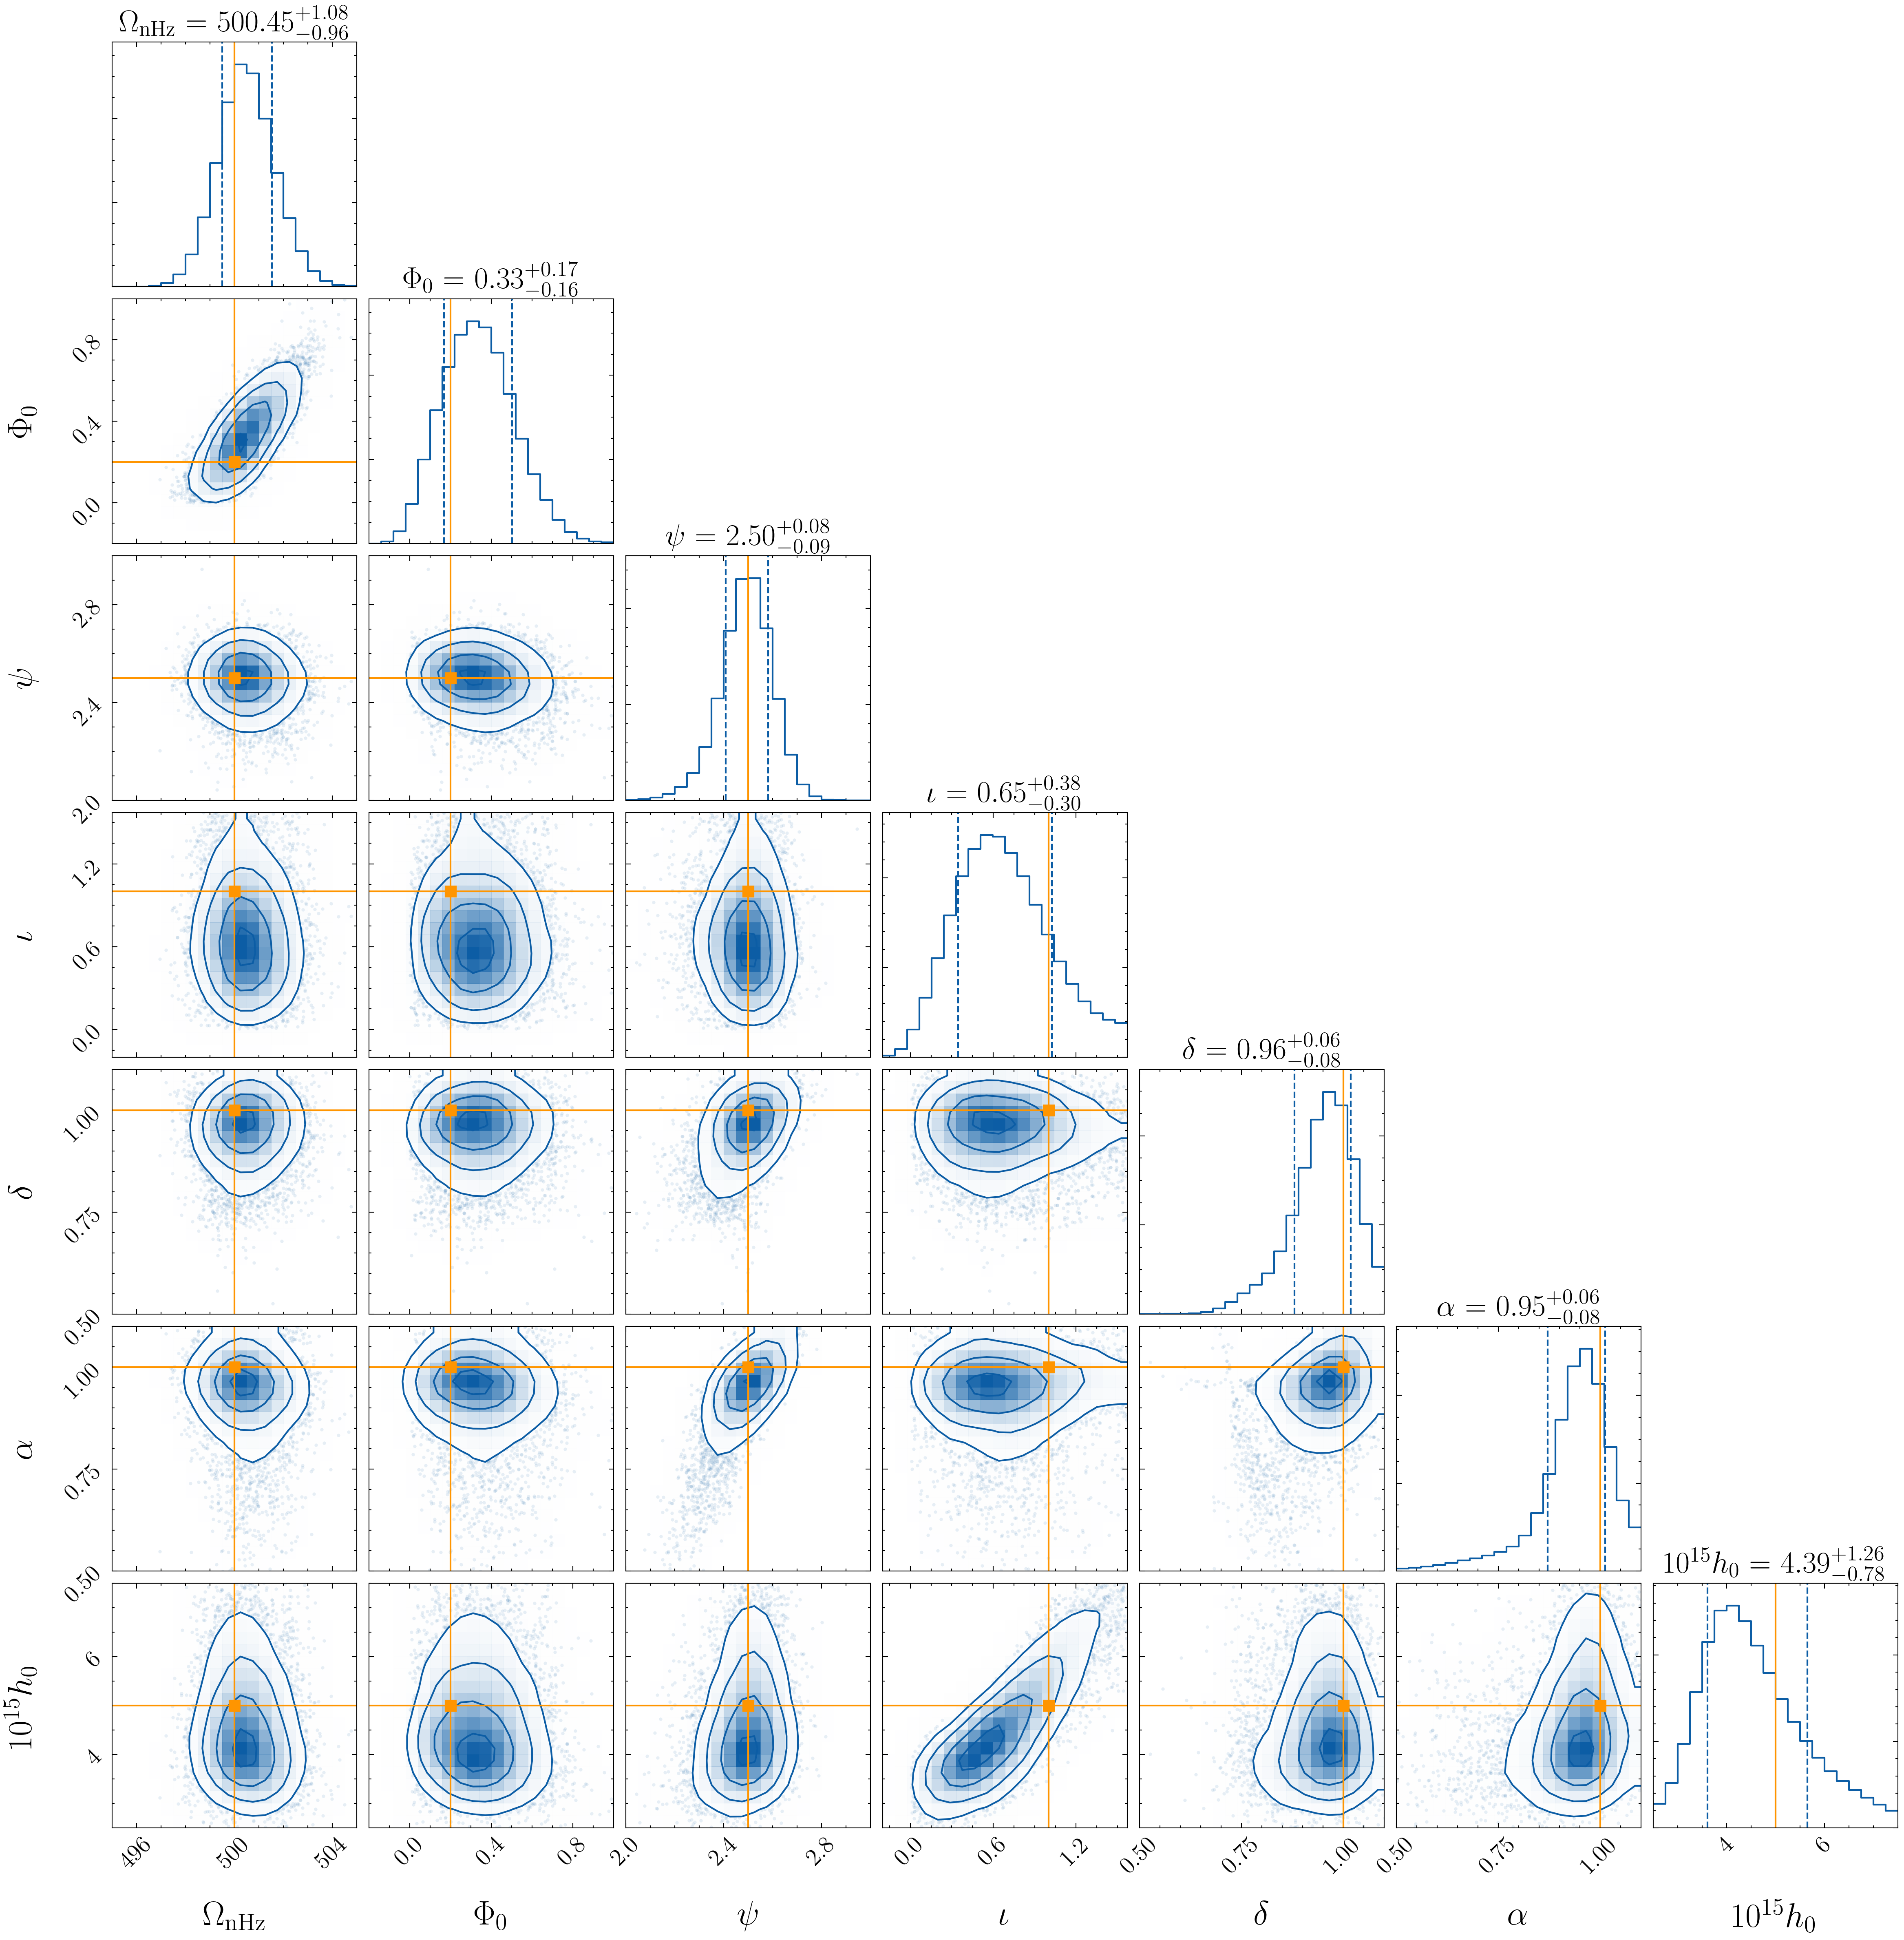
\includegraphics[width=\textwidth, height =\textwidth ]{images/small_h_posterior_10}
	\caption{Posterior distribution for the GW source parameters $\boldsymbol{\theta}_{\rm gw}$ for the representative system described in Table \ref{tab:parameters_and_priors}, for a single realisation of the system noise. The vertical orange lines indicate the true injected values. The contours in the 2D histograms denote the (0.5, 1, 1.5, 2)-$\sigma$ levels. \DIFaddbeginFL \DIFaddFL{The subtitles of the marginalized 1D posteriors denote the posterior median and the 0.16,0.84 quantiles. }\DIFaddendFL We are able to accurately estimate each parameter of interest. We plot the scaled variables $\Omega_{\rm nHz} = \Omega \times 10^{9}$ Hz and $h_{0, \times 10^{15}} = h_0 \times 10^{15}$. Note that the $x$-axis scaling does not span the total prior space.}
	\label{fig:corner_plot_1}
\end{figure*}

%\begin{figure*}
%	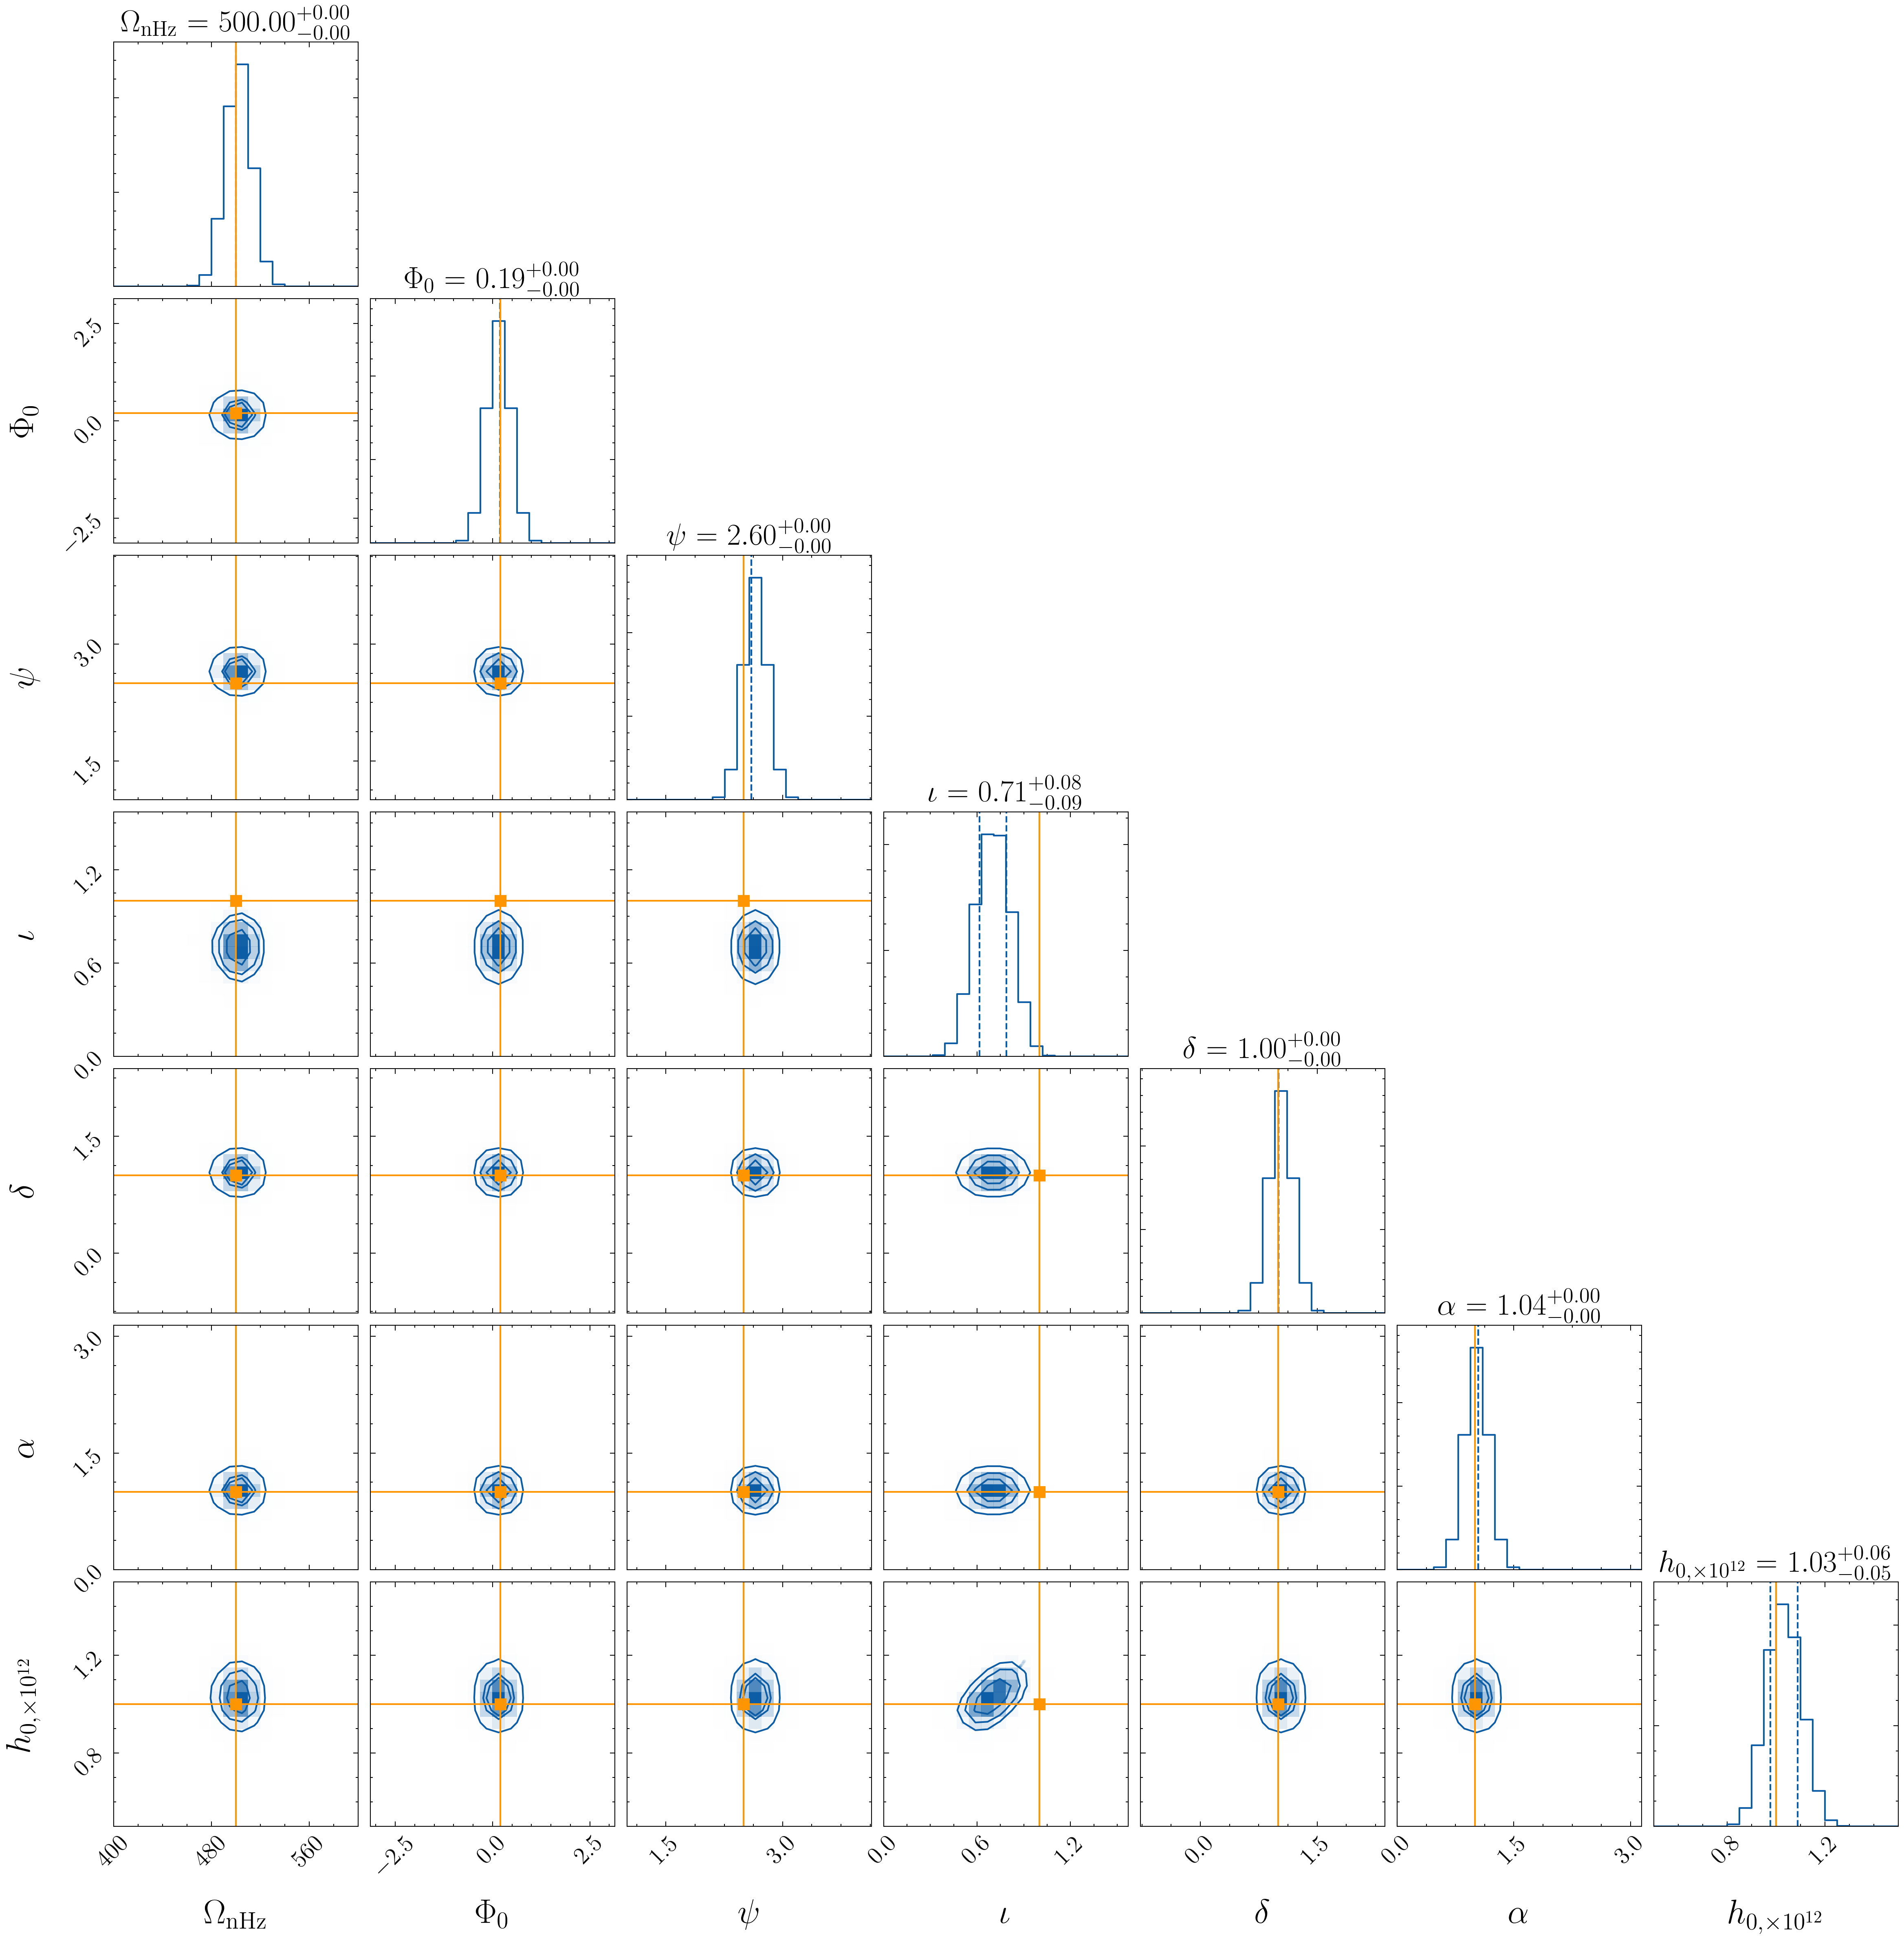
\includegraphics[width=\textwidth, height =\textwidth ]{images/representative_example_v2_GW}
%	\caption{Posterior distribution for the GW source parameters $\boldsymbol{\theta}_{\rm gw}$ for the representative system described in Table \ref{tab:parameters_and_priors}, for a single realisation of the system noise. The vertical orange lines indicate the true injected values. The contours in the 2D histograms denote the (0.5, 1, 1.5, 2)-$\sigma$ levels. We are able to accurately estimate each parameter of interest. We pot the scaled variables $\Omega_{\rm nHz} = \Omega \times 10^{9}$ Hz and $h_{0, \times 10^{12}} = h_0 \times 10^{12}$.}
%	\label{fig:corner_plot_1}
%\end{figure*}



\DIFdelbegin \subsubsection{\DIFdel{Multiple noise realisations}} %DIFAUXCMD
\addtocounter{subsubsection}{-1}%DIFAUXCMD
\DIFdelend \DIFaddbegin \subsection{\DIFadd{Multiple noise realisations}} \DIFaddend \label{sec:multiple_noise}
\begin{figure*}
	\DIFdelbeginFL %DIFDELCMD < 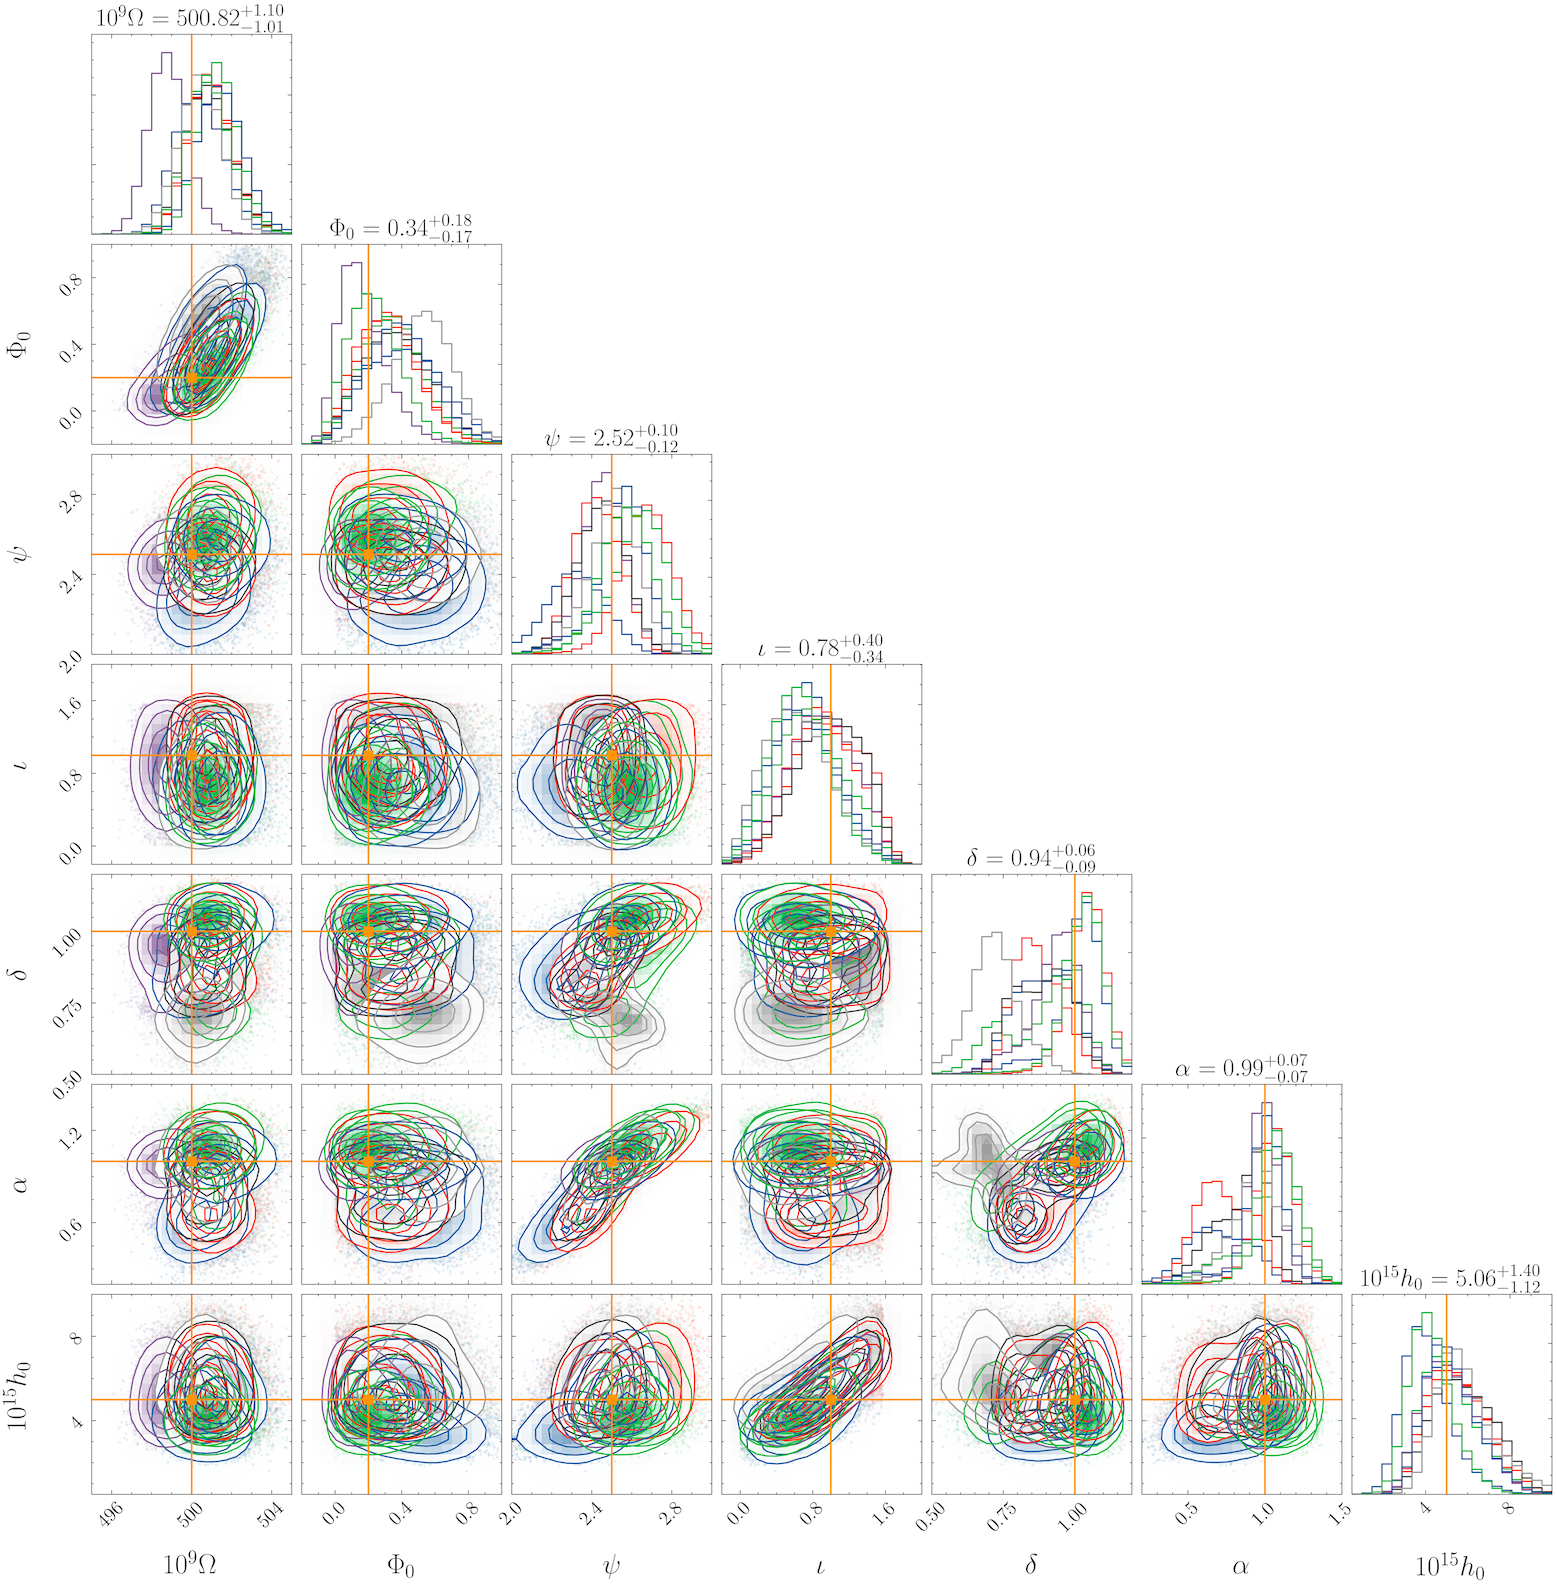
\includegraphics[width=\textwidth, height =\textwidth]{images/stacked_GW_plot_small_h_definitive2}
%DIFDELCMD < 	%%%
\DIFdelendFL \DIFaddbeginFL \includegraphics[width=\textwidth, height =\textwidth]{images/stacked_GW_plot_small_h_definitive3}
	\DIFaddendFL \caption{As Figure \ref{fig:corner_plot_1} but for nine realisations of the noise processes. The \DIFaddbeginFL \DIFaddFL{subtitles of the marginalized 1D posteriors refer to values for the median posterior across the noise realisations. The }\DIFaddendFL injection value is generally contained within the 90 \% credible interval for the vast of majority posteriors. The inferred posterior distributions show strong agreement between the different noise realisations for the majority of static parameters. A slight skew-bias is apparent in some of the parameters, e.g. $\iota$. Correlations can be seen between $\Omega - \Phi_0$, $\psi-\alpha$ and $\iota - h_0$.} 
	\label{fig:corner_plot_2}
\end{figure*}
\begin{table}
	\centering
	\begin{tabular}{ccll}
		\toprule
		Parameter & Injected Values & Units & $W_{1, \rm median}$  \\
		\hline
		$\Omega$     &   $5 \times 10^{-7}$ & Hz & $10^{-9}$ \\
		$\Phi_0$          & $0.20$ & rad & $0.13$ \\
		$\psi$              & $2.50$ & rad & $0.16$ \\
		$\iota$             & $1.0$ & rad & $0.14$ \\ 
		$\delta$              & $1.0$  & rad & $0.09$ \\
		$\alpha$          & $1.0$  & rad & $0.17$\\
		$h_0$            & $5 \times 10^{-15}$ & - & $8 \times 10^{-16}$ \\
		\bottomrule
	\end{tabular}
	\caption{Median value of the Wasserstein distance $W_{1, \rm median}$, for each parameter, calculated across the $10^3 \choose 2$ pairs of probability posteriors, for the the $10^3$ noise realisations in Figure \ref{fig:pairwise_wasserstein}. $W_{1, \rm median}$  sets the bound on the difference in expectation value between the one dimensional posteriors, and is generally small with respect to the width of the prior space.}
	\label{tab:Wasserstein}
\end{table}
\begin{figure*}
	\setkeys{Gin}{width=\linewidth}   

	\begin{subfigure}[b]{0.22\textwidth}
		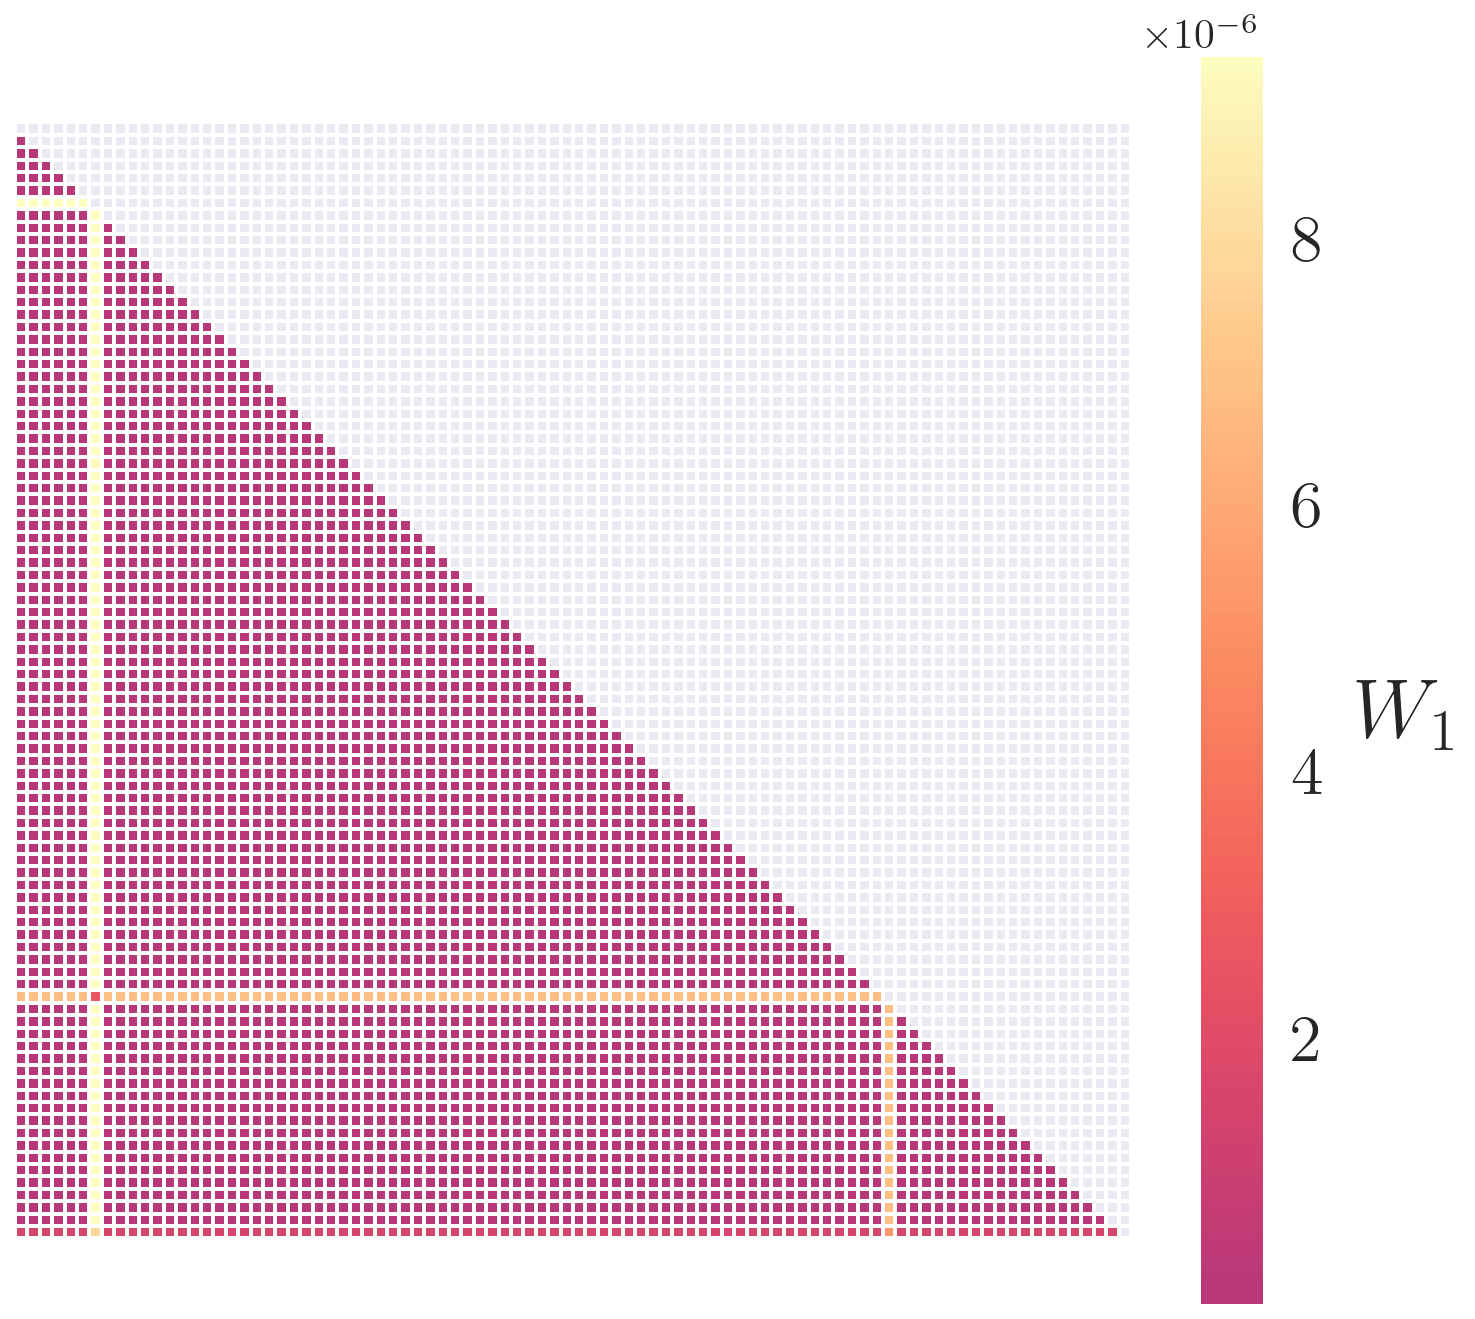
\includegraphics[width=\textwidth]{images/WD_0}
		\caption{$\Omega$}
	\end{subfigure}
	\hfill
	\begin{subfigure}[b]{0.22\textwidth}
		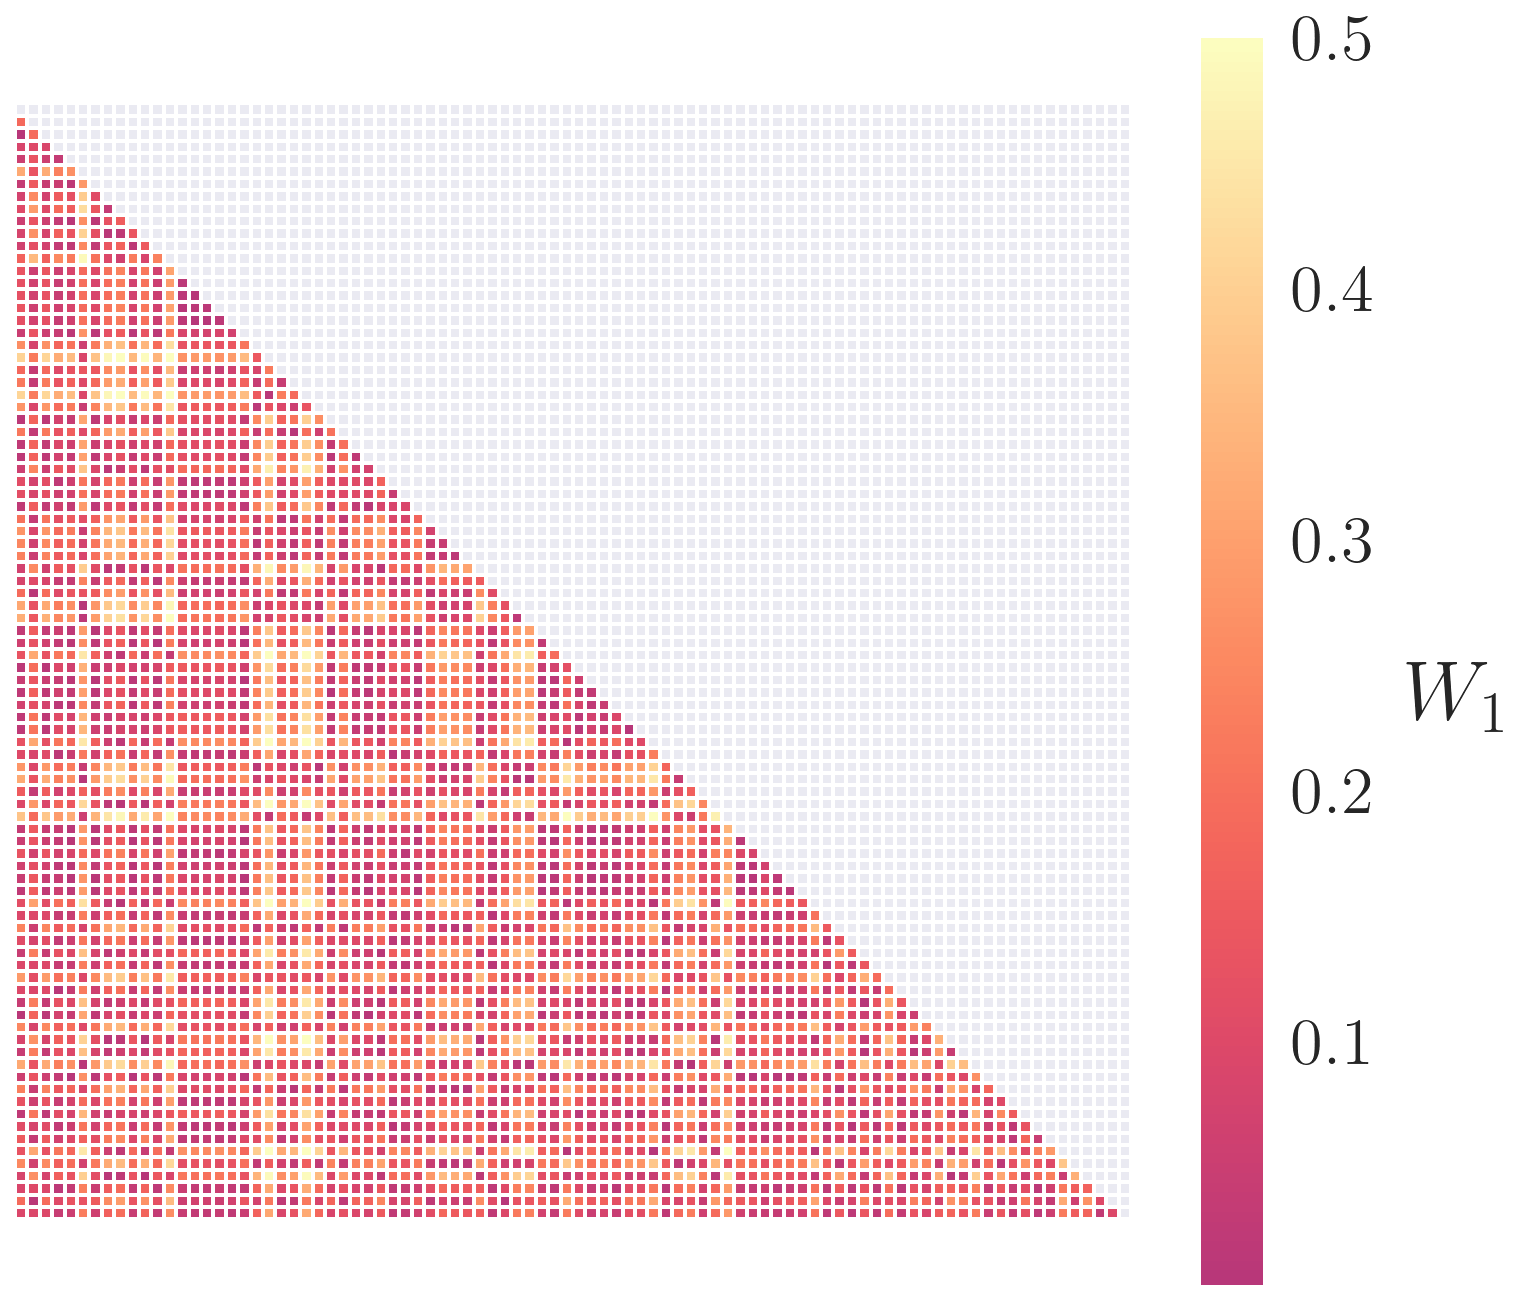
\includegraphics[width=\textwidth]{images/WD_1}
		\caption{$\Phi_0$}
	\end{subfigure}
	\hfill	
	\begin{subfigure}[b]{0.22\textwidth}
		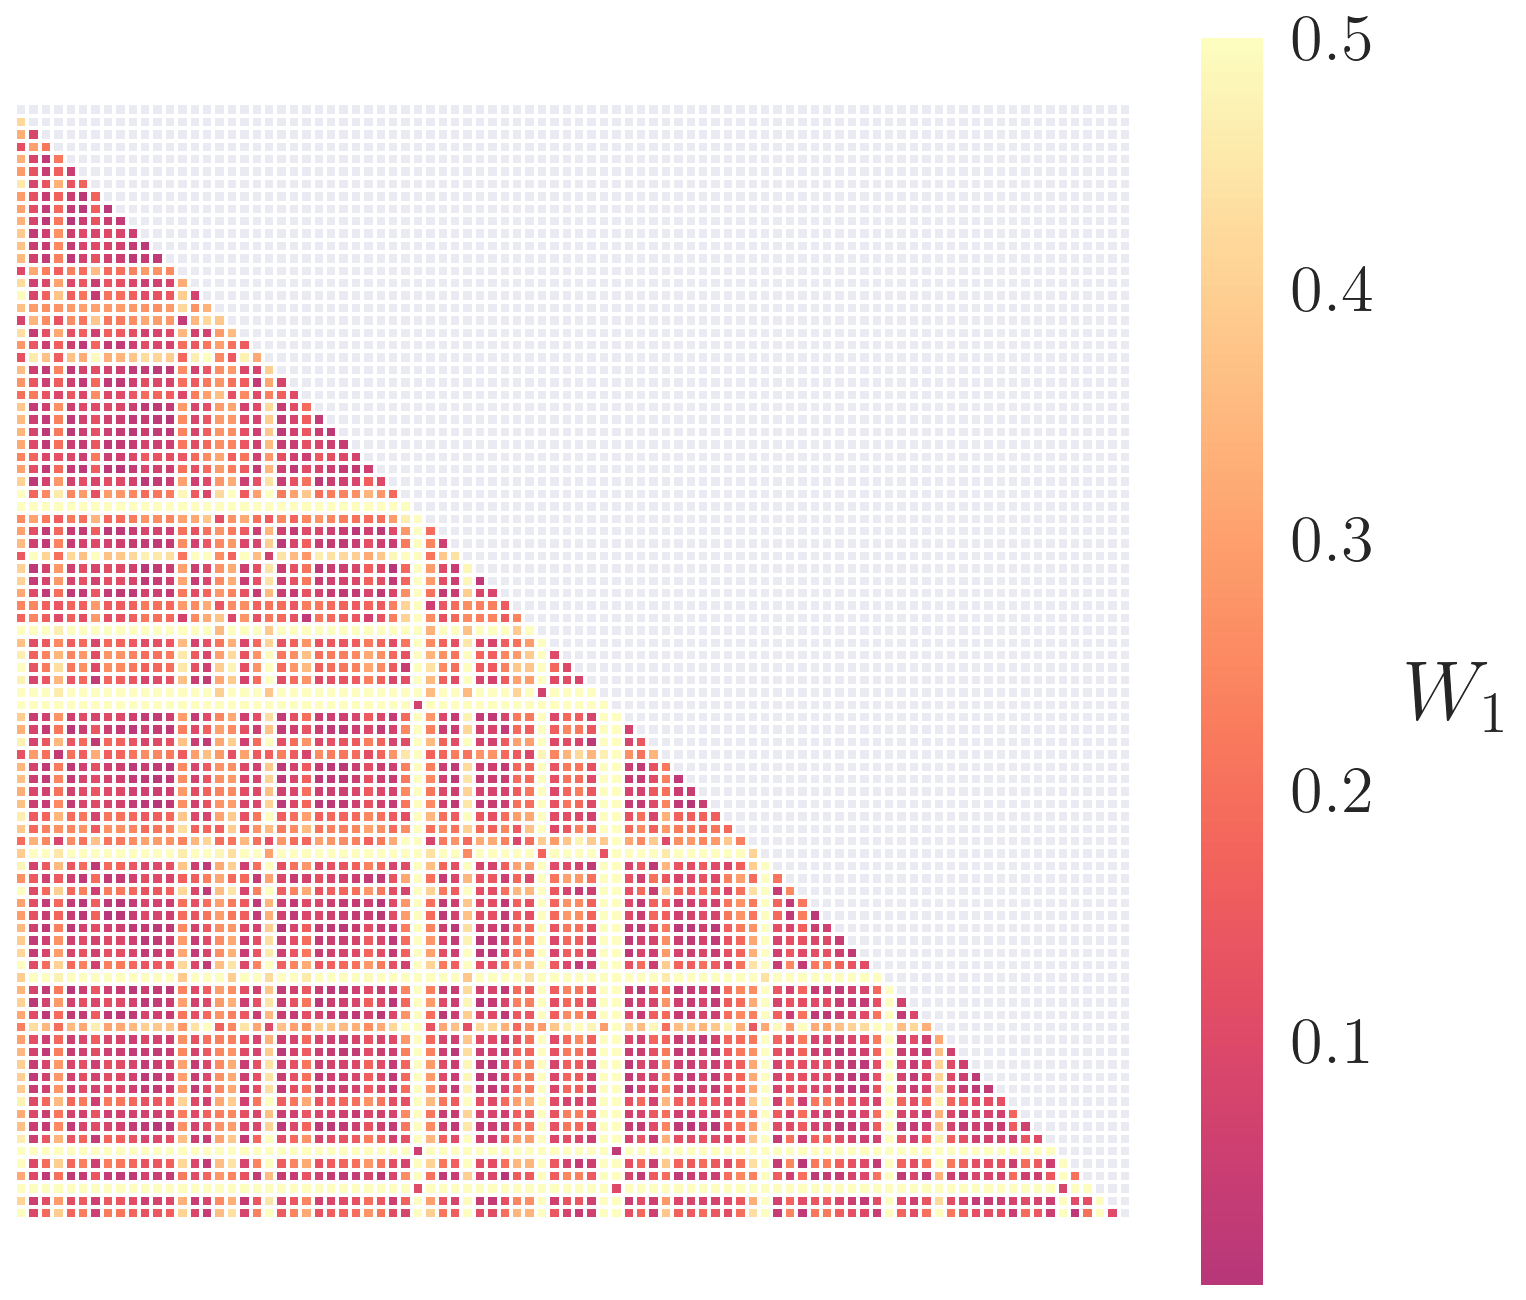
\includegraphics[width=\textwidth]{images/WD_2}
		\caption{$\psi$} \label{figWD_psi}
	\end{subfigure}
	\hfill
	\begin{subfigure}[b]{0.22\textwidth}
		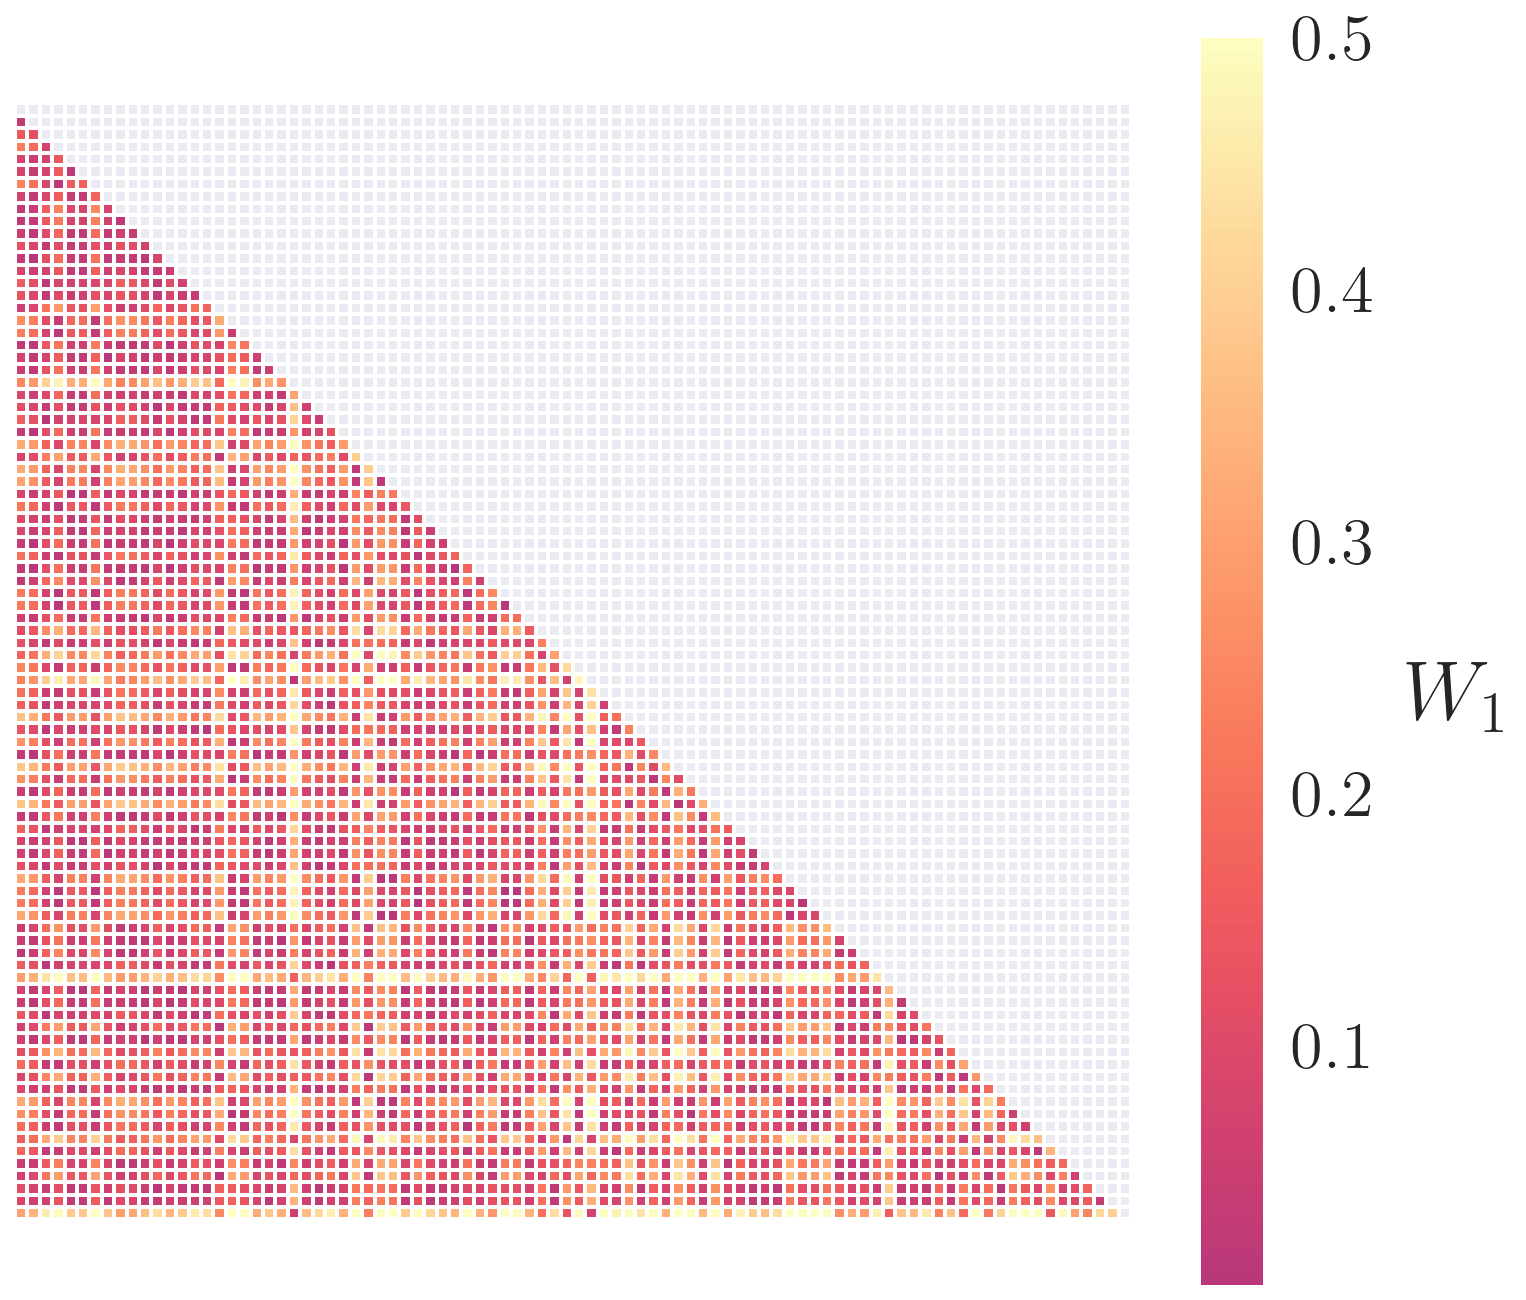
\includegraphics[width=\textwidth]{images/WD_3}
		\caption{$\iota$}
	\end{subfigure}
	\medskip
	\begin{subfigure}[b]{0.3\textwidth}
		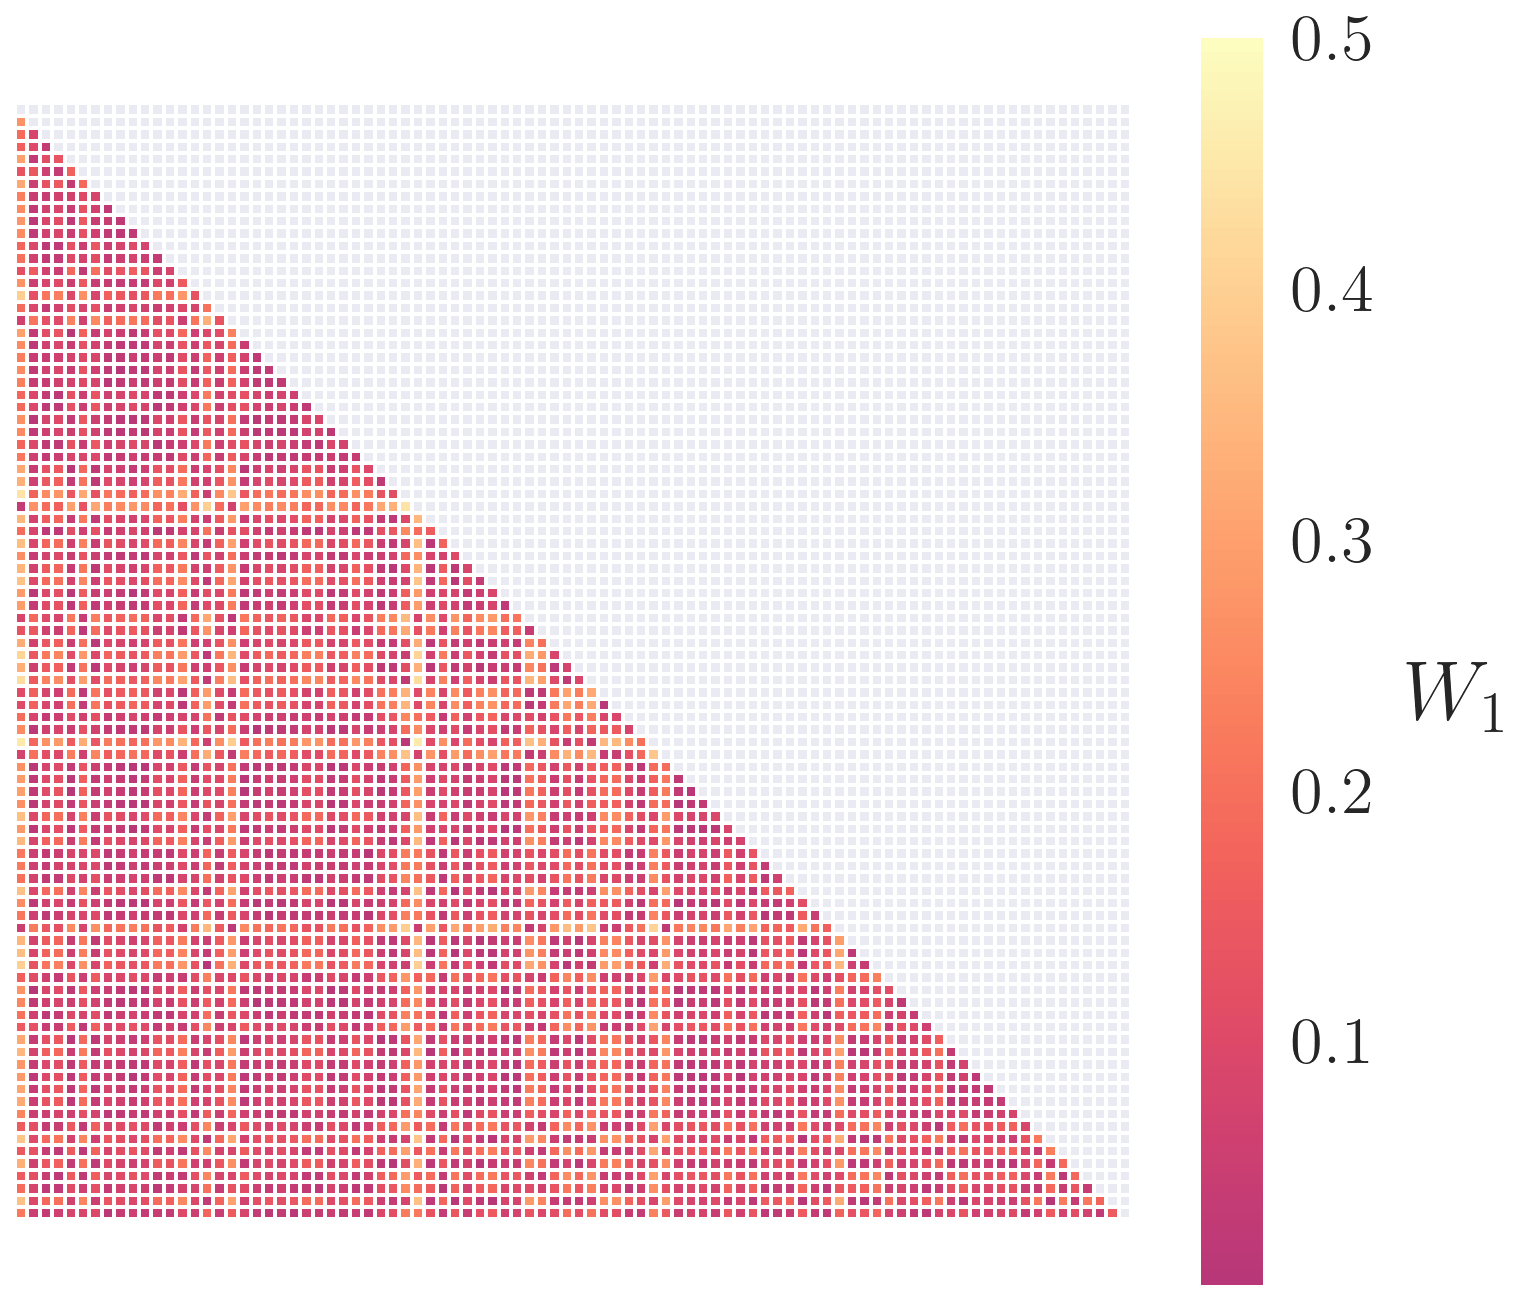
\includegraphics[width=\textwidth]{images/WD_4}
		\caption{$\delta$}
	\end{subfigure}
	\hfill	
	\begin{subfigure}[b]{0.3\textwidth}
		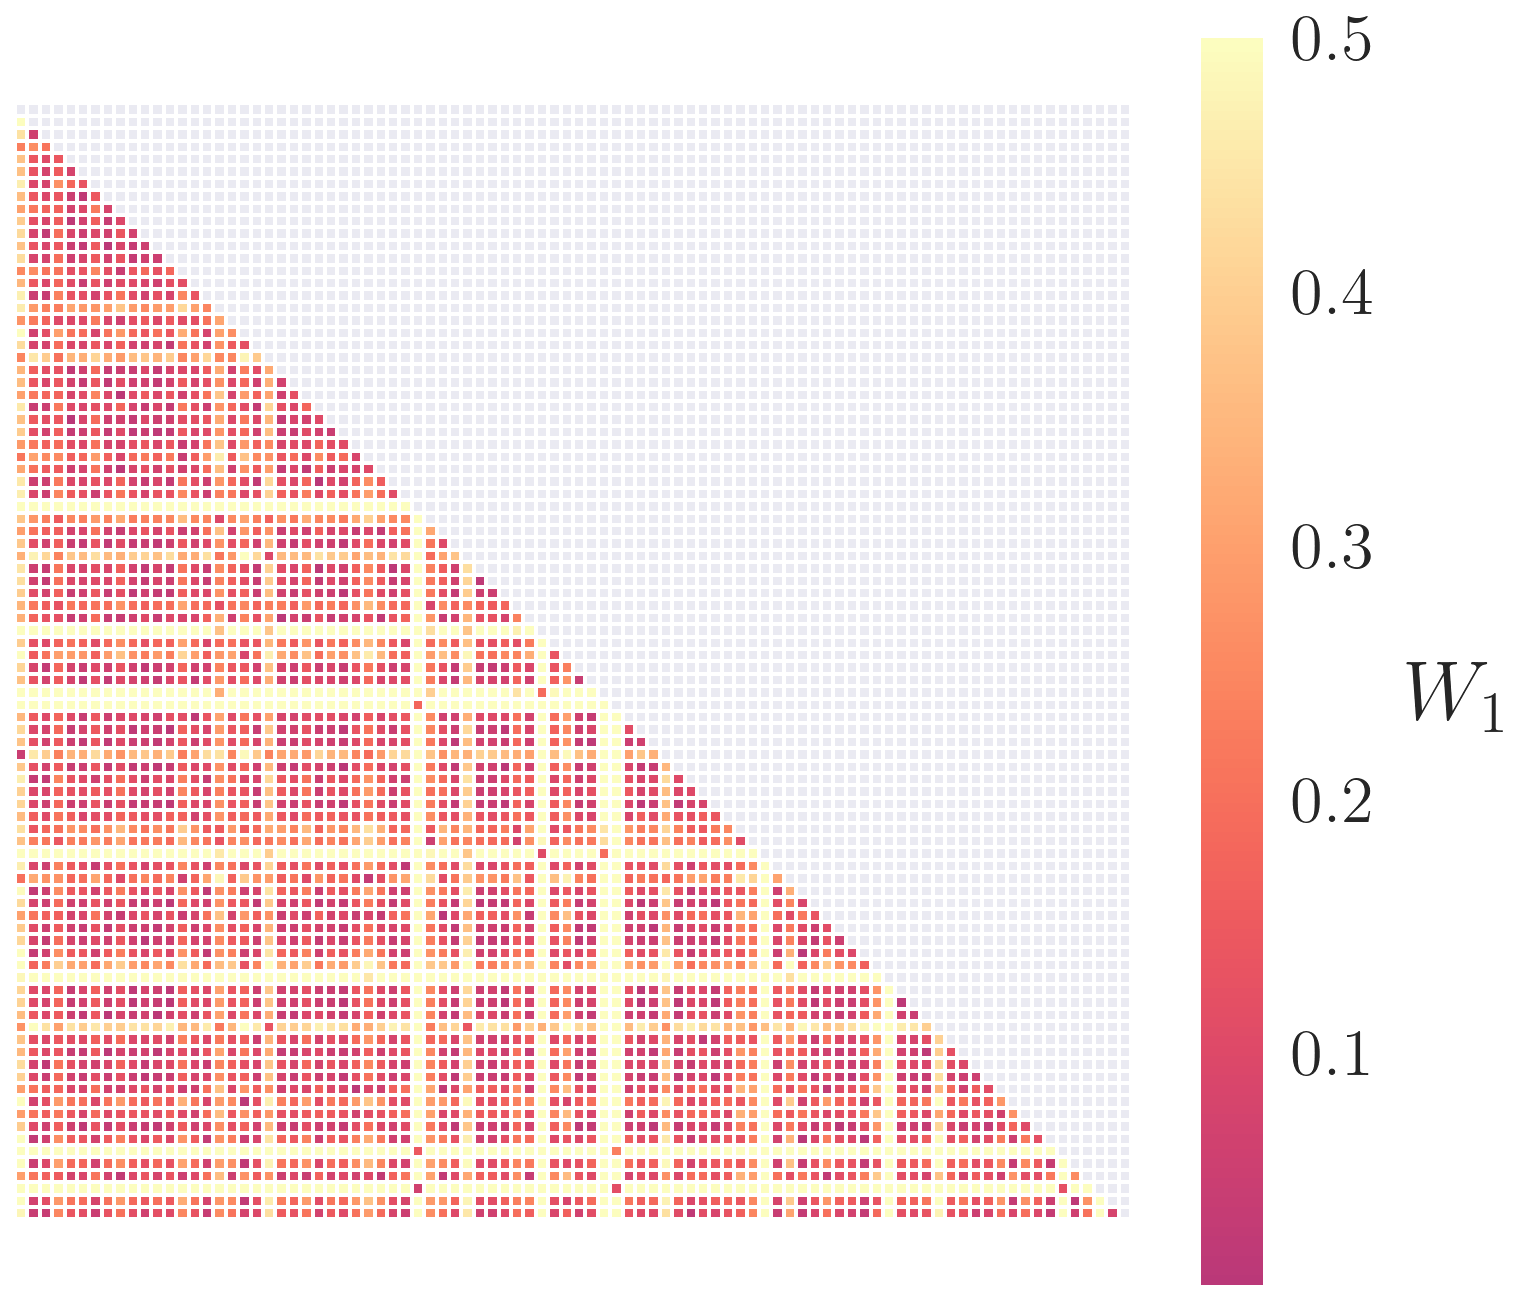
\includegraphics[width=\textwidth]{images/WD_5}
		\caption{$\alpha$}
	\end{subfigure}
	\hfill	
	\begin{subfigure}[b]{0.3\textwidth}
		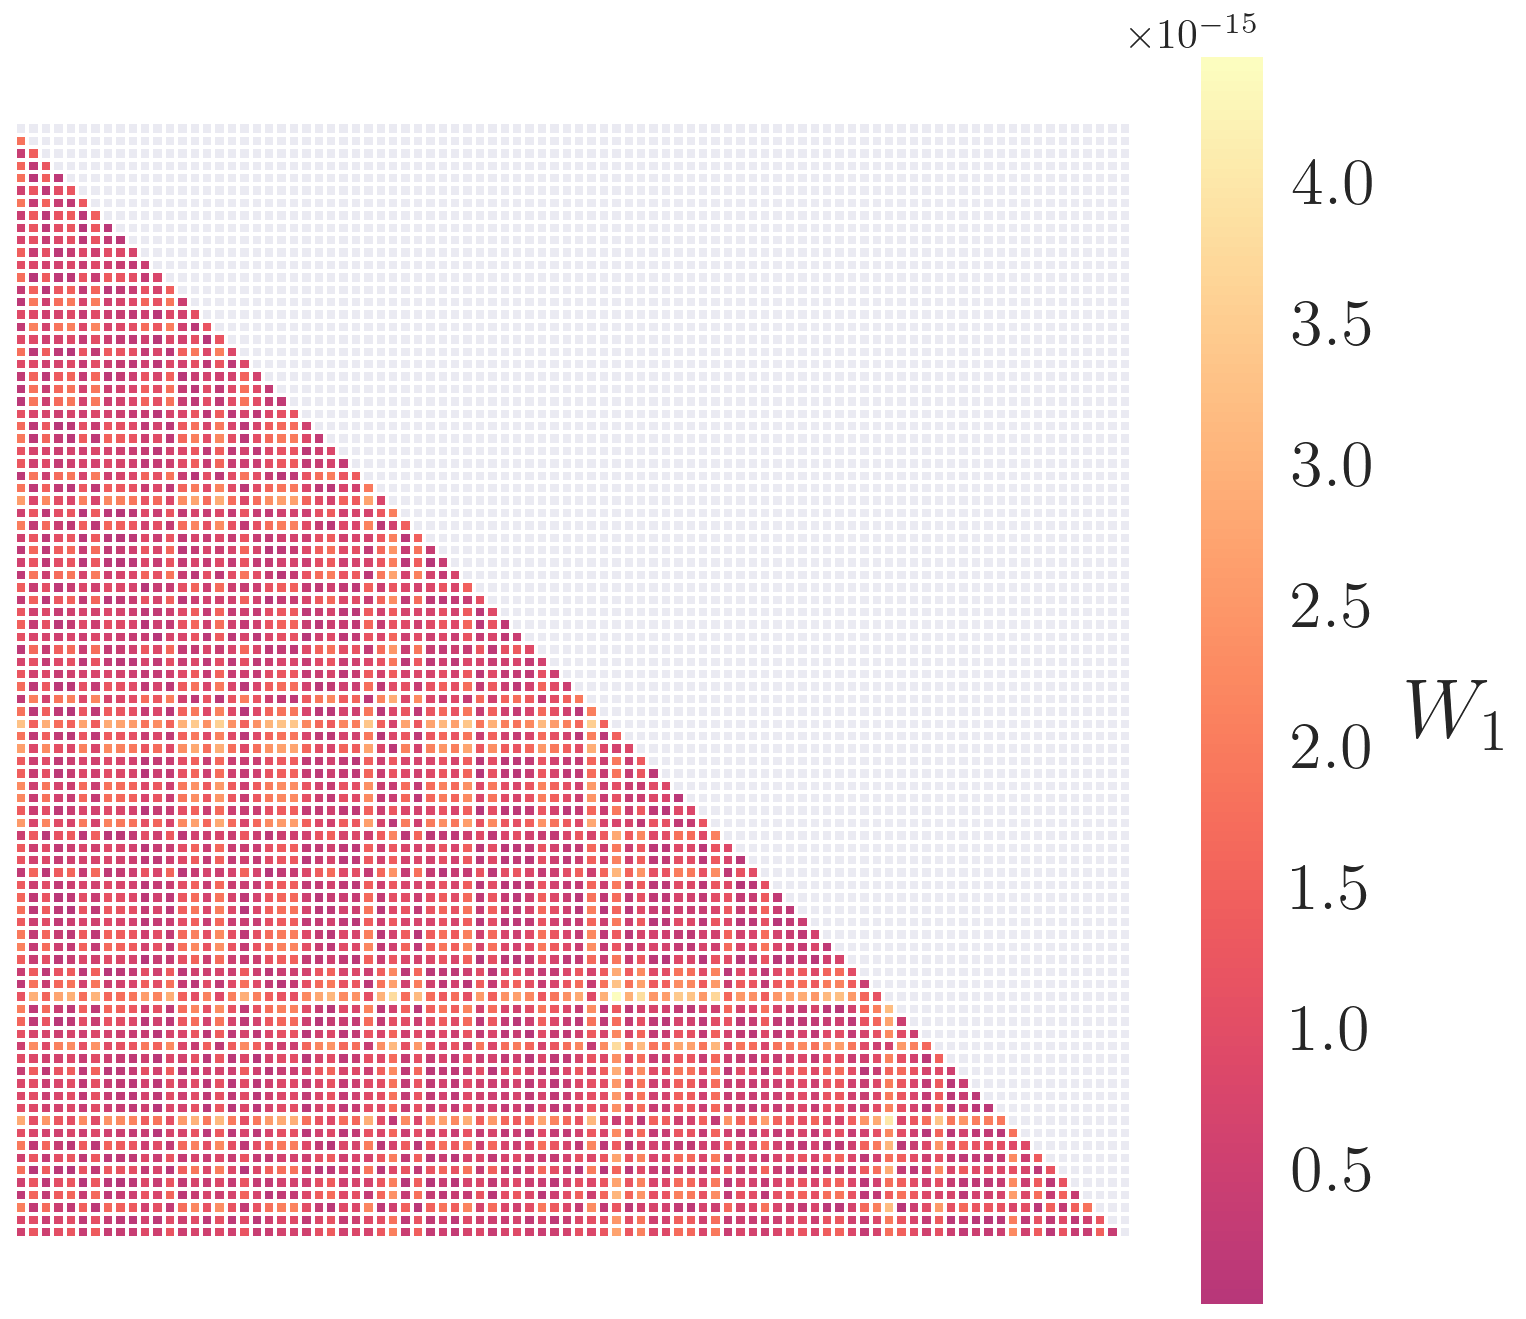
\includegraphics[width=\textwidth]{images/WD_6}
		\caption{$h$}
	\end{subfigure}
	\caption{The first moment of the Wasserstein distance, $W_1$, calculated between each pair of one-dimensional posteriors for our representative system across $10^3$ realisations, for each parameter of $\boldsymbol{\theta}_{\rm gw}$  $W_1$ provides an upper bound on the difference in expected values between any two probability distributions. $W_1$ is generally small across all parameters and all posteriors, but some posteriors converge poorly leading to large values of $W_1$. The $W_1$ values inferred for $\psi$ and $\alpha$ are strongly correlated with correlation coefficient = 0.96. An example noise realisation with particularly large pairwise $W_1$ values is labelled with an asterisk in (c) and is discussed in the text.} \label{fig:pairwise_wasserstein}
\end{figure*}
\begin{figure}
	\centering
	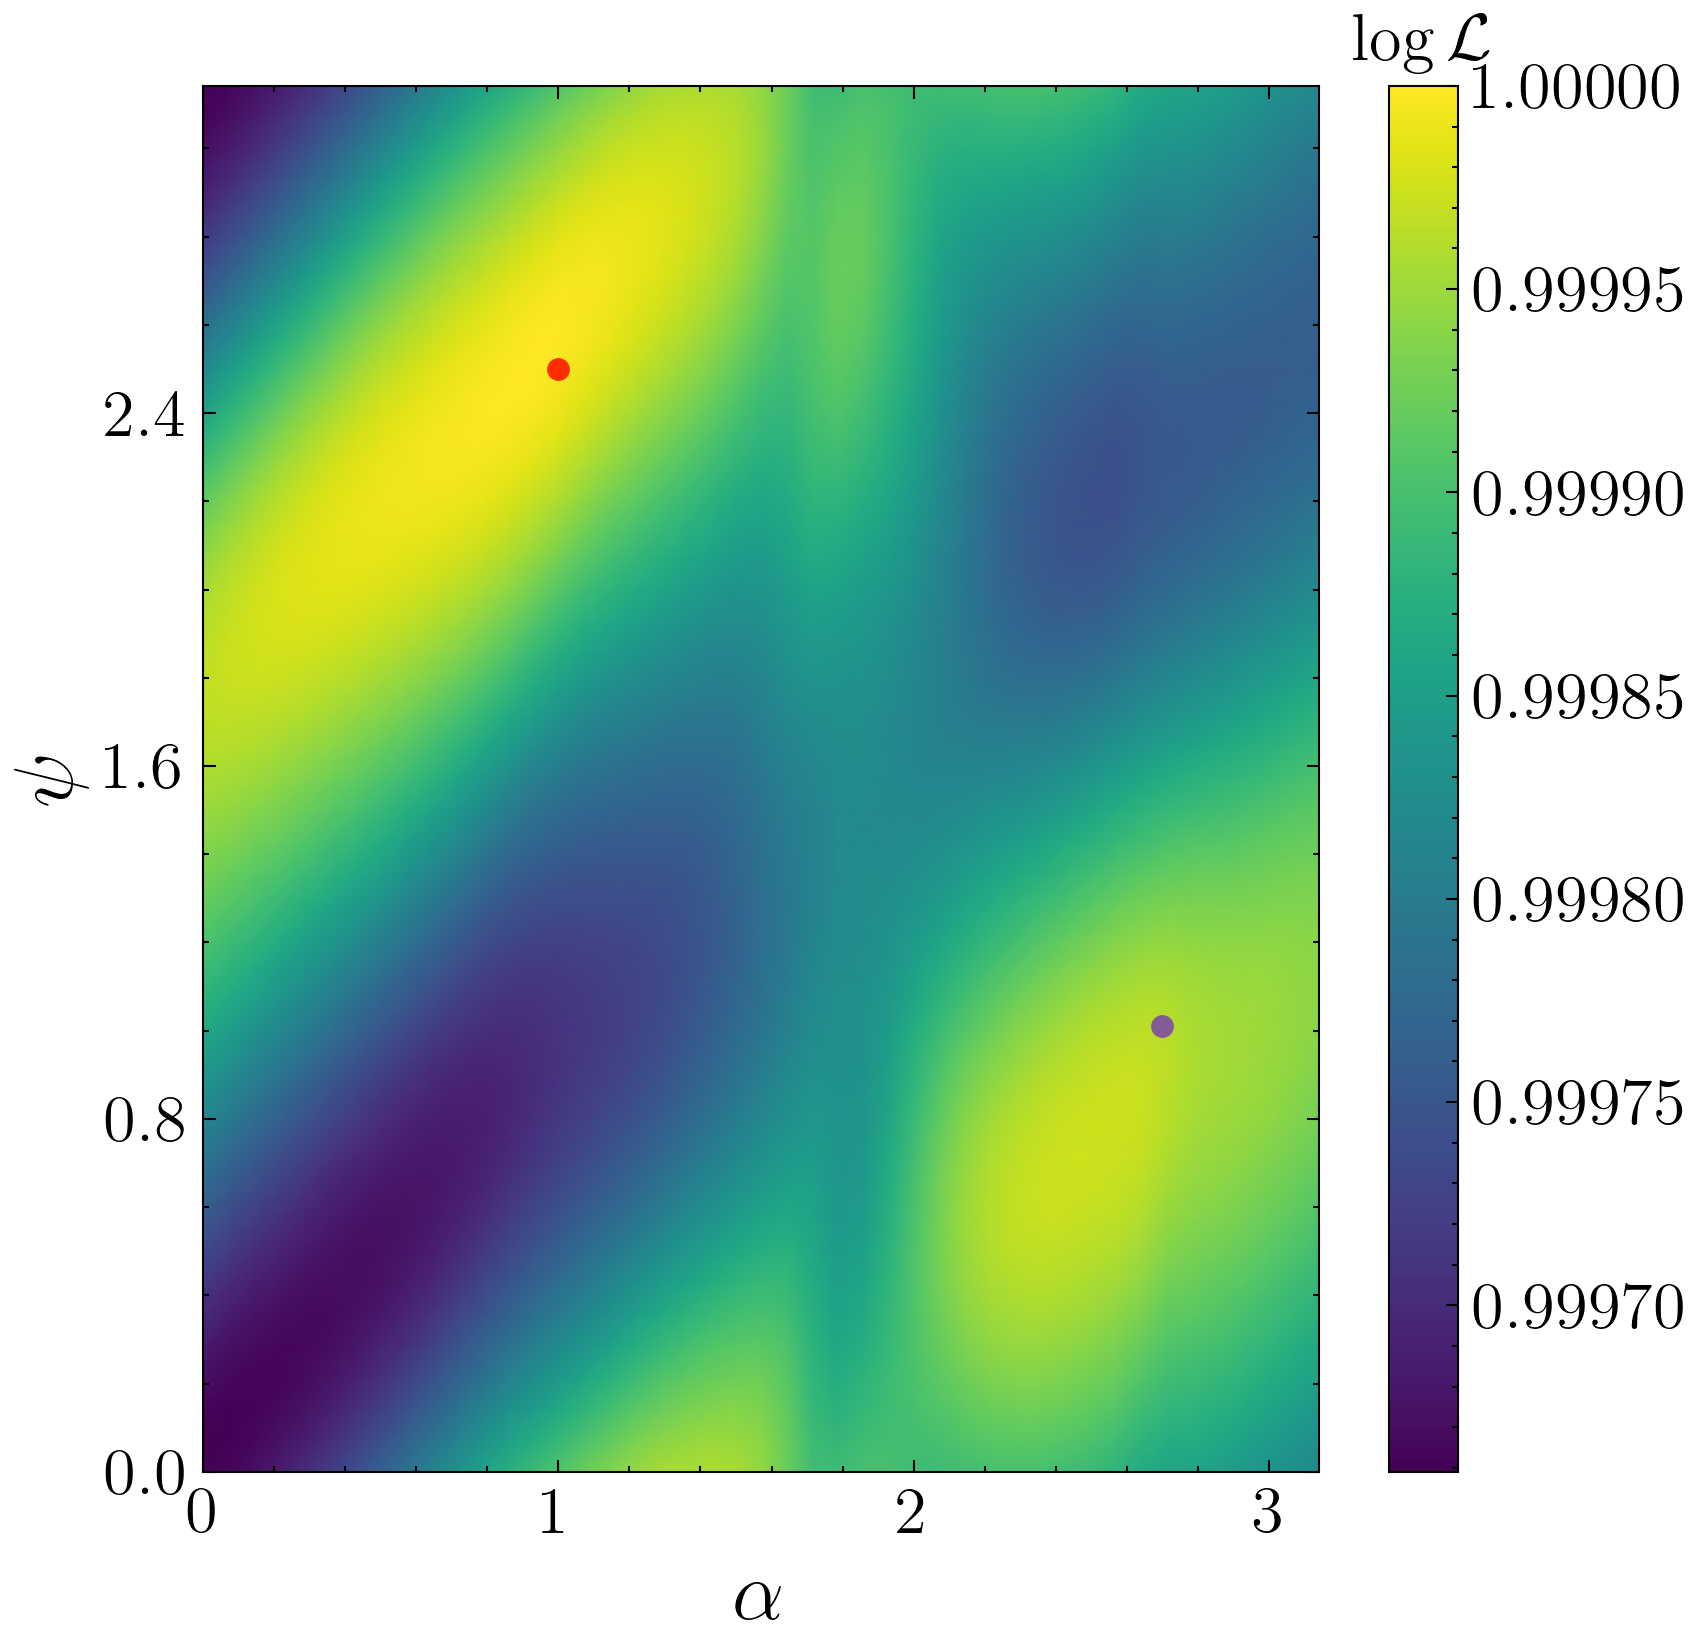
\includegraphics[width=\columnwidth]{images/likelihood_surface_alpha_psi}
	\caption{Log-likelihood, $\log \mathcal{L}$ (Equation \ref{eq:likelihood}) surface across the $\alpha-\psi$ parameter space for a single noise realisation.  The red point labels the location of the maxima, and the magenta point labels the the median values of the one-dimensional posteriors inferred for a particular noise realisation of the data. The likelihood has been normalised with respect to the absolute value of the maxima. A multi-modal structure is clearly visible and for this noise realisation the nested sampler has settled in the local optima. This can be solved generally by increasing the number of live points $n_{\rm live}$.}
	\label{fig:likelihood_surface_alpha_psi}
\end{figure}
The above example was for a single realisation of the noise processes. It is important to confirm that our method is robust against different realisations of the noise and that the specific realisation of the noisy data used in Section \ref{sec:parameter_estim} is not particularly advantageous or convenient for our method. In this Section we confirm that we are able to infer comparable results for different noise realisations. To this end we take our representative example from Table \ref{tab:parameters_and_priors} and generate $1000$ \DIFdelbegin \footnote{%DIFDELCMD < \tiny%%%
\DIFdel{\textcolor{red}{TK: For the results plotted here we currently just do 100 noise realisations. 1000 is a hangover when we were using a larger strain ($h=10^{-12}$) as our canonical example. The $10^3$ noise realisations are currently running and plots will be updated once completed, but I don't expect any meaningful changes \textcolor{red}{;for $h=10^{-12}$ the results/conclusions of 100 realisations are the same as 1000 realisations)}}}%DIFDELCMD < \normalsize%%%
} %DIFAUXCMD
\addtocounter{footnote}{-1}%DIFAUXCMD
\DIFdelend realisations of the process noise and measurement noise. For each realisation of the data we can then independently estimate the static parameters, $\boldsymbol{\theta}$. In Figure \ref{fig:corner_plot_2} we show the results for the  estimated values of $\boldsymbol{\theta}_{\rm gw}$ for nine realisations of the noise. This figure is analogous to the single noise realisation of Figure \ref{fig:corner_plot_1}. We plot only nine realisations of the noise rather than the full set of 1000 realisations so as to not overcrowd the figure. As in Section \ref{sec:parameter_estim} the estimates of $\boldsymbol{\theta}_{\rm psr, reduced}$ are recovered unambiguously across the 1000 noise realisations and for brevity we do not show the results here. \newline 


We can see from Figure \ref{fig:corner_plot_2} that the results from these 9 noise realisations agree well with the single realisation result that we saw in  Figure \ref{fig:corner_plot_1}. Considering the one-dimensional marginalized posteriors, the inferred probability distributions of the parameters broadly overlap across the different noise realisations. For the vast majority of parameters and noise realisations the injected value is contained within the 90\% credible interval. As in the single noise case, there are tentative signs of bias for some of the parameters, with the one-dimensional posteriors not symmetric about the injected value. For example, the maximum a posteriori probability estimates of $\iota$ across the noise realisations all appear left-skewed, consistently underestimating the injected value. Given the uncertainty in the posteriors it is difficult to draw strong conclusions on a potential bias and this question will be discussed in detail in Section \ref{sec:bias} \newline 


We now consider the complete set of $10^3$ noise realisations, rather than the subset of nine realisations in the preceding discussion. For each realisation of the noise, for each parameter, we infer a marginalised one-dimensional posterior. Our goal is to compare these posteriors between different noise realisations and evaluate whether our method can consistently and reliably converge to comparable posteriors. To this end we use the the Wasserstein distance \citep[WD;][]{Wasserstein,Villani2009} from optimal transport theory which defines an intuitive notion of similarity between probability distributions. \footnote{\DIFdelbegin \DIFdel{\textcolor{red}{\tiny TK: How much of the following is ok, how much to move to the appendix? I don't want to get bogged down in WD and distract from astro arguments but we use $W_1$ as metric so I feel like it should be defined in the main body of the text, and the bounding result is important...} }\DIFdelend \DIFaddbegin \DIFadd{\textcolor{red}{\tiny TK: How much of the following Wasserstein stuff is ok here, how much to move to the appendix? I don't want to get bogged down in WD and distract from astro arguments, but we use $W_1$ as metric so I feel like it should be defined in the main body of the text, and the bounding result is important...} }\DIFaddend \normalsize} The WD is a popular metric in machine learning \citep{2017arXiv170107875A}, climate modelling \citep{2022JCli...35.1215P,2023QJRMS.149..843K}, computational biology \citep{GONZALEZDELGADO2023168053} and geophysics \citep{2023GeoRL..5003880M}. A full review of the Wasserstein distance, which may be unfamiliar to some readers, is presented in Appendix \ref{sec:wasserstein}. The WD is the cost of an optimal strategy for moving probability mass between two distributions from position $x$ to position $y$, with respect to some cost function $c(x,y)$. Throughout this work we use the first moment of the Wasserstein distance, $W_1(\mu,\nu)$, which is defined between one-dimensional probability distributions $\mu$ and $\nu$ as
\begin{eqnarray}
	W_1(\mu,\nu)=  \inf_{\lambda \in \Gamma(\mu, \nu)} \int |x-y| d \lambda (x,y) \ ,
\end{eqnarray}
where $\lambda(x,y)$ is the transport plan, $\Gamma(\mu, \nu)$ is the set of all couplings of $\mu$ and $\nu$ and $ |x-y|$ defines the cost function. \DIFdelbegin %DIFDELCMD < \newline 
%DIFDELCMD < 

%DIFDELCMD < %%%
\DIFdel{For each parameter in $\boldsymbol{\theta}_{\rm gw}$ we calculate $W_1$ between every pair of posteriors across our $10^3$ noise realisations. The results are presented in Figure \ref{fig:pairwise_wasserstein} which shows the $W_1$ value for each pair of posteriors. The }\DIFdelend \DIFaddbegin \DIFadd{The }\DIFaddend first moment of the WD has a \DIFdelbegin \DIFdel{useful }\DIFdelend \DIFaddbegin \DIFadd{convenient }\DIFaddend physical interpretation given by the Monge-Kantorovich duality \citep{villani2003topics,Villani2009}:
\begin{eqnarray}
	| \boldsymbol{E}(X_{\mu} )-\boldsymbol{E}(Y_{\nu} ) | \leq W_1(\mu, \nu) \ , \label{eq:WDdefn}
\end{eqnarray}
where $X_{\mu}$ and $Y_{\nu}$ are random variables of the distributions $\mu$ and $\nu$ respectively, and $\boldsymbol{E}$ denotes the expected value. We can see that $W_1$ bounds the difference in the expected values. \DIFdelbegin \DIFdel{That is to say, if $W_1 =0.5$ rad between }\DIFdelend \DIFaddbegin \DIFadd{Taking a concrete example, suppose that we infer }\DIFaddend two one-dimensional posterior distributions \DIFdelbegin \DIFdel{estimated for e.g. }\DIFdelend \DIFaddbegin \DIFadd{for }\DIFaddend $\iota$, \DIFdelbegin \DIFdel{this }\DIFdelend \DIFaddbegin \DIFadd{for two different realisations of the noise, and calculate $W_1 =0.5$ rad between them. This }\DIFaddend means that the difference in the expected \DIFdelbegin \DIFdel{values in }\DIFdelend \DIFaddbegin \DIFadd{value of two }\DIFaddend random variables drawn from \DIFdelbegin \DIFdel{these distributions }\DIFdelend \DIFaddbegin \DIFadd{the two posteriors }\DIFaddend is no greater than $0.5$ rad. \DIFdelbegin \DIFdel{From Figure \ref{fig:pairwise_wasserstein}it is }\DIFdelend \DIFaddbegin \newline 


\DIFadd{For each parameter in $\boldsymbol{\theta}_{\rm gw}$ we calculate $W_1$ between every pair of posteriors across our $10^3$ noise realisations. The results are presented in Figure \ref{fig:pairwise_wasserstein}. The figure shows a lower triangular heat-map where each point denotes the $W_1$ value between a pair of posteriors. Small values of $W_1$ are magenta moving to red for large values of $W_1$. Note that the heat-map colour scaling is not the same for all subplots of the figure. It is }\DIFaddend evident that $W_1$ is generally small across all pairs of posteriors. We define $W_{1, \rm median}$ as the median value of $W_1$ across all $10^3 \choose 2$ pairs of noise realisations. The values of $W_{1, \rm median}$ for each parameter are quoted in Table \ref{tab:Wasserstein}. As a percentage of the width of the prior space (e.g. for $\alpha$ the width of the prior is $2 \pi$), the median $W_1$ for each parameter is $\lesssim 3 \%$. Generally speaking, the method converges to consistent one-dimensional posteriors for each parameter across different noise realisations. \newline 

There are a small fraction of the total number of noise realisations which have a large Wasserstein distance from all the other posteriors of all the other noise realisations. These are the strong yellow lines in Figure \ref{fig:pairwise_wasserstein}. These correspond exclusively to posteriors which have converged poorly and not found the likelihood global maximum. For instance, the top strong horizontal yellow line in Figure \ref{figWD_psi}, which is identified by an asterisk in the figure, corresponds to a posterior for $\psi$ which has converged sub-optimally, with an estimated value of $\psi = 1.01 \pm 0.06$ rad, highly diverged from the true injected value of $2.50$ rad. The $W_1$ \DIFaddbegin \DIFadd{value }\DIFaddend between this posterior and all the posteriors inferred for all other noise realisations is $\sim 1.7$ radians. We also observe a strong correlation across all noise pairs (Pearson correlation coefficient $=0.96$) between the $W_1$ inferred for $\alpha$ and $\psi$, indicating that noise realisations which corrupt the inference of $\psi$ similarly affect $\alpha$. This is due to multimodal likelihood surface for $\psi-\alpha$, shown in Figure \ref{fig:likelihood_surface_alpha_psi}. We can see that the likelihood surface has a global optima at the approximate location of the injected values ($\alpha \sim 1.0$, $\psi\sim2.5$) and local optima that corresponds to the location of the example poorly converged posterior discussed previously, with $\psi = 1.01$ rad. This problem of poor global convergence can be solved in principle by increasing the number of live points $n_{\rm live}$ in the nested sampler so as to better cover the likelihood surface and prevent falling into local minima. 




\DIFdelbegin \subsubsection{\DIFdel{Detection}} %DIFAUXCMD
\addtocounter{subsubsection}{-1}%DIFAUXCMD
\DIFdelend \DIFaddbegin \subsection{\DIFadd{Detection}} \DIFaddend \label{sec:detection}
We frame the problem of claiming a detection of a GW in the noisy data in terms of a Bayesian model selection procedure as described in Section \ref{sec:model_selection}. $\mathcal{M}_1$ is the Earth-terms only model, i.e. the state-space model with a Kalman filter using Equation \eqref{eq:measuremen_earth}. The Bayes factor, $\beta$, as defined in Equation \eqref{eq:bayes} is presented in Figure \ref{fig:bayes} for our representative system, where we now vary the magnitude of the GW strain, $h_0$. The noise processes in the synthetic data are identical realisations for each value of $h_0$; the only change in the data is the change in $h_0$. We can see that for $\beta >10$ there is an approximate log-linear relationship between $\beta$ and $h_0$ where the GW source is easily detectable with decisive evidence ($\beta \sim 100$) for $h_0 \gtrapprox 10^{-14}$. We take $\beta = 10$ as a tolerance cut-off above which we can accept $\mathcal{M}_1$ and claim a detection of the GW. For this system, given this realisation of the noise, the minimal detectable strain is $\sim 3.9 \times 10^{-15}$. This minimal detectable strain is of course particular to this system and will be influenced in general by e.g. $T_{\rm obs}$, $\sigma_{\rm m}$ as well as the parameters of the GW source such as its location on the sky. \newline 

There is an evident sparsity and steep drop-off of $\beta$ for values of \DIFdelbegin \DIFdel{$h_0 \lesssim 3.9 \times10{-15}$}\DIFdelend \DIFaddbegin \DIFadd{$h_0 \lesssim 3.9 \times10^{-15}$}\DIFaddend . The steep drop off is due to the two competing models becoming increasingly indistinguishable as the strain signal decreases and the measurement noise starts to dominate. The sparsity is due some of the $\beta$ value becoming negative at these points.This is a noise artefact of the nested sampling method. For these points the noise in the sampler starts to dominate, the sampler converges sub-optimally, and the hierarchical relationship between $\mathcal{M}_0$ and  $\mathcal{M}_1$ fails. That is, the requirement that $\mathcal{Z}(\boldsymbol{Y} | \mathcal{M}_1) > \mathcal{Z}(\boldsymbol{Y} | \mathcal{M}_0)$ no longer holds. There is nothing special about these particular points; if one recreates the $\beta - h_0$ curve by rerunning the nested sampler these sparse locations appear at different values of $h_0$, for $\beta < 10$. For $\beta > 10$ the sampling noise is sufficiently small with respect to the signal and the model hierarchy holds. Increasing the number of live points $n_{\rm live}$ used by the nested sampler improves the performance at small values of $h_0$ since as discussed in Section \ref{sec:nested_sampling} the uncertainties in $\mathcal{Z}$ scale as $\mathcal{O}(1/ \sqrt{n_{\rm live}})$. For the results presented in this subsection we set $n_{\rm live} =2000$. 
\begin{figure}
	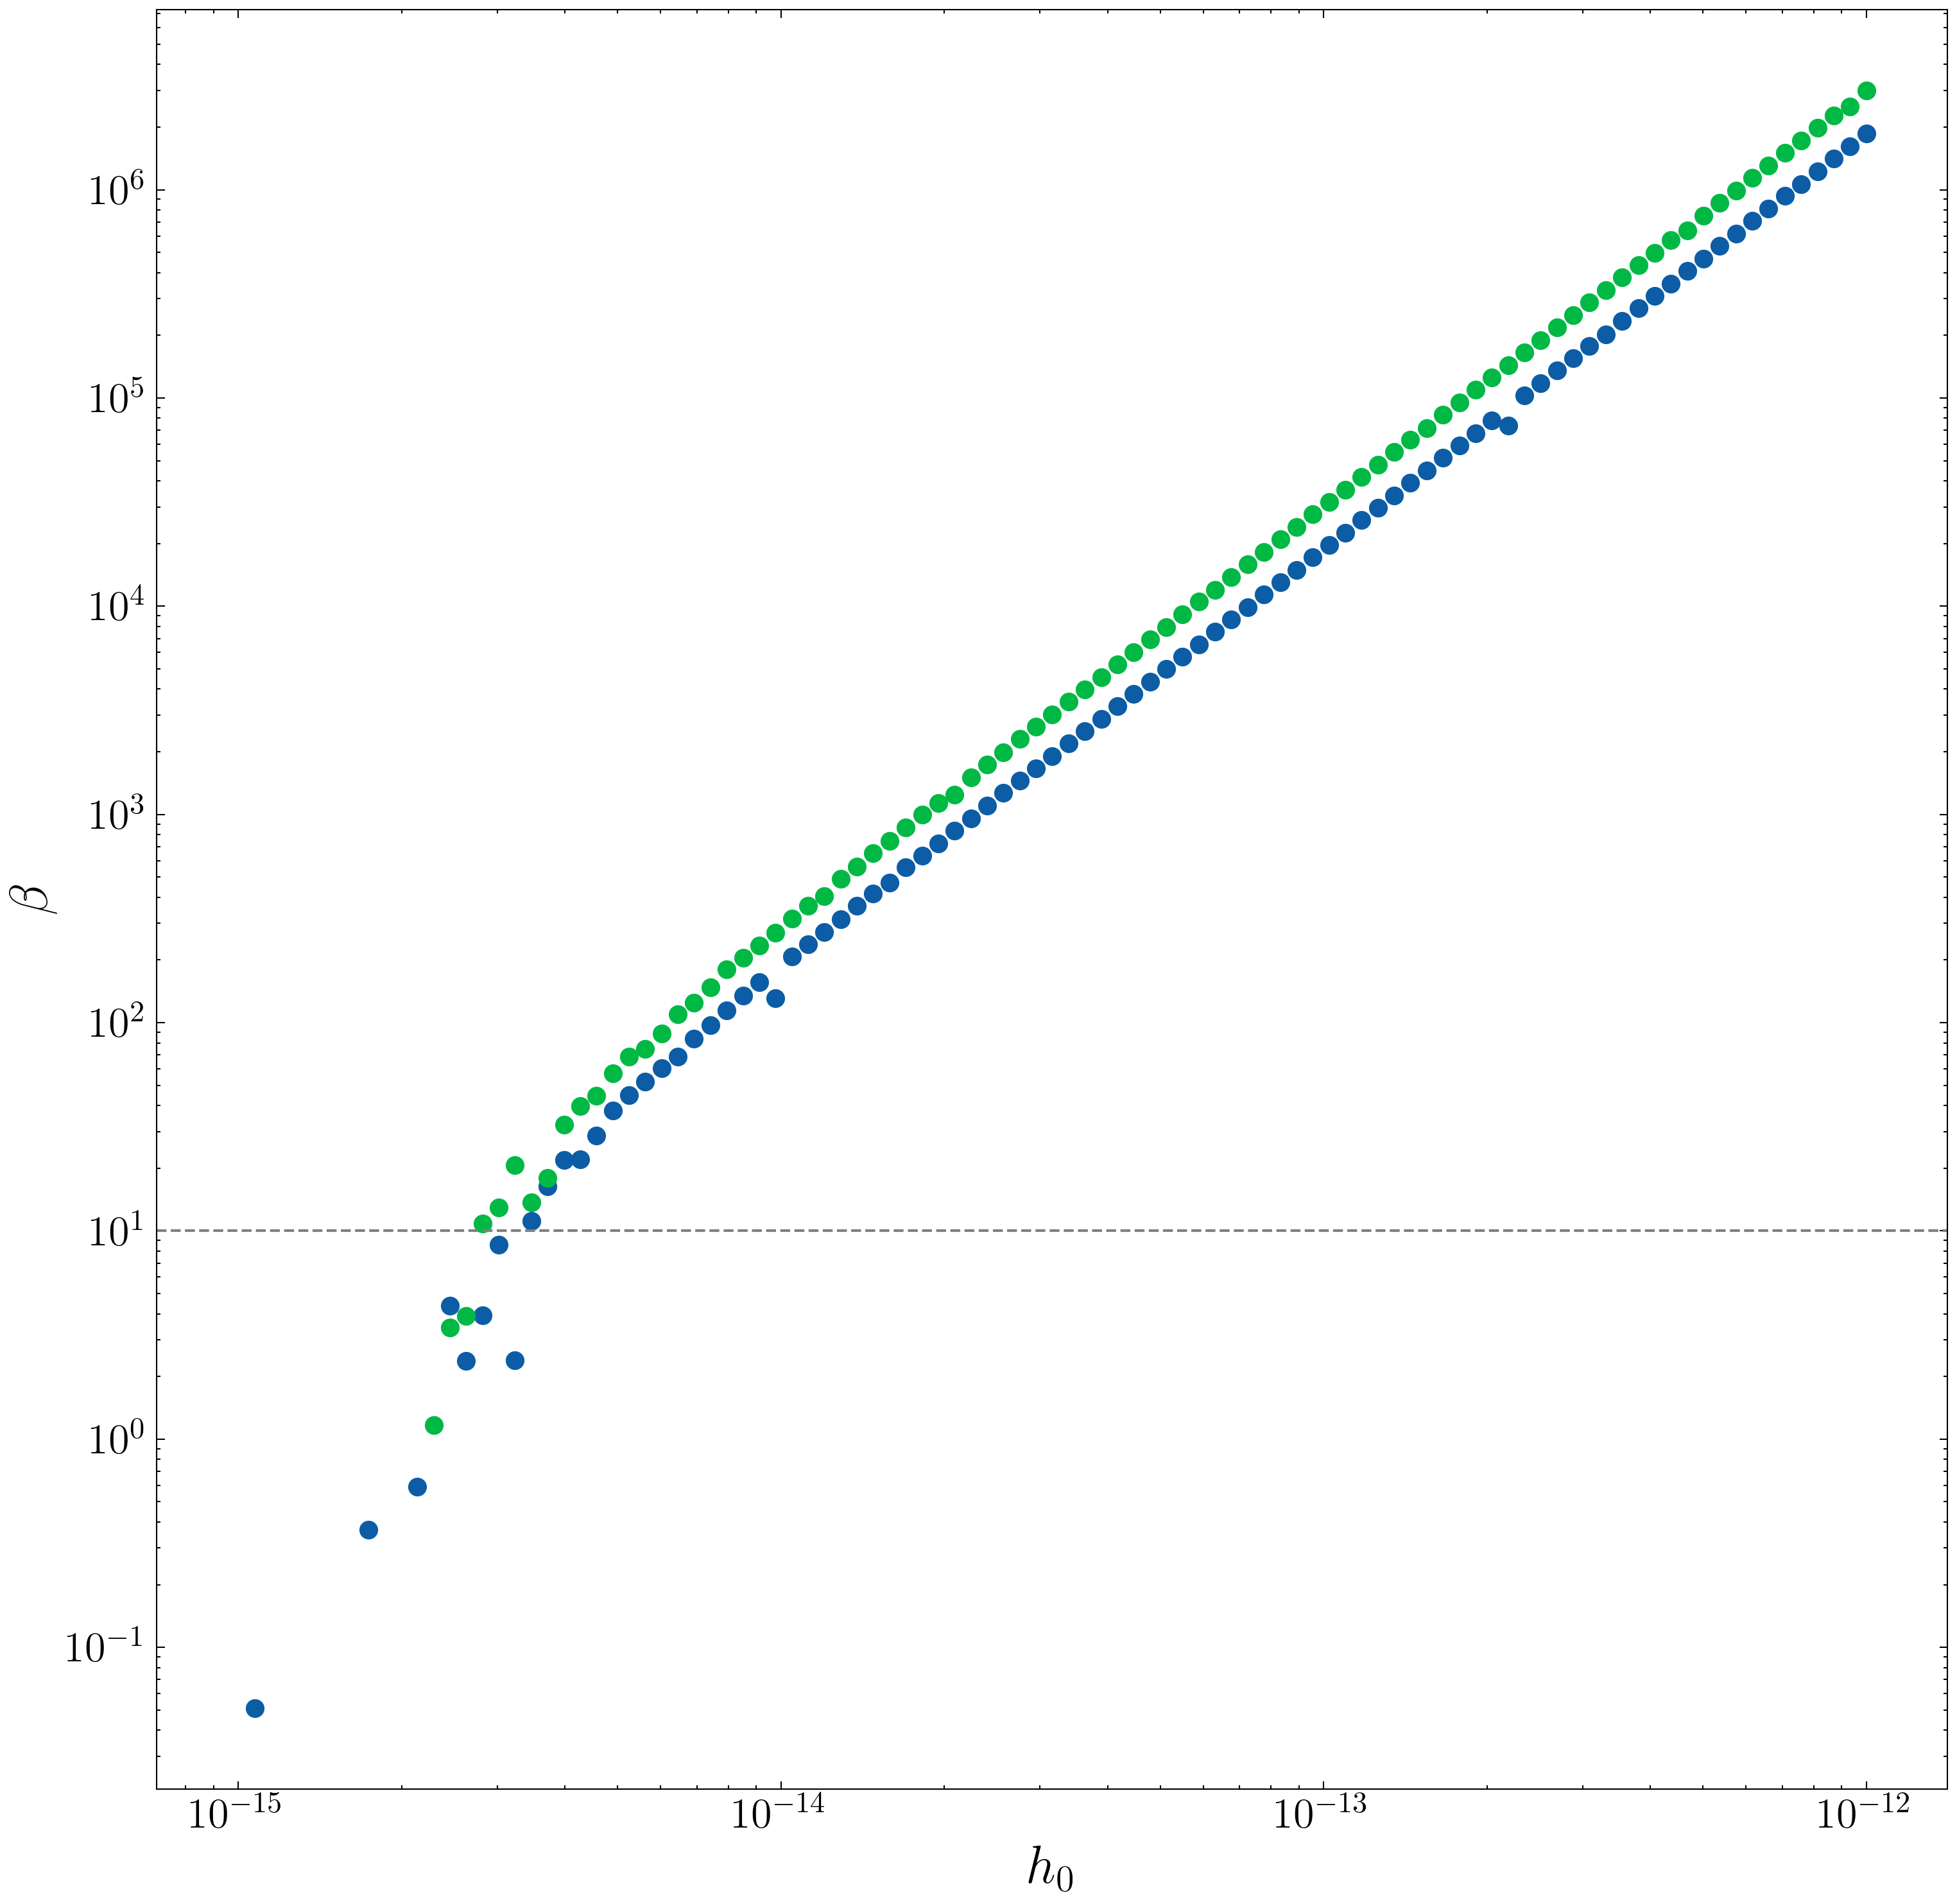
\includegraphics[width=\columnwidth]{images/CanonicalBayesPlot2000}
	\caption{Bayes ratio $\beta$ between the competing models $\mathcal{M}_1$ (GW present in data) and $\mathcal{M}_0$ (GW not present in data) at different GW strain magnitudes $,h_0$, for the representative example summarised in Table \ref{tab:parameters_and_priors}. The horizontal grey dashed line labels the detection threshold of $\beta = 10$. The minimal detectable strain, below which $\beta < 10$, is $\sim 3.9 \times 10^{-15}$. Gaps in the data below $\beta=10$ occur due to noise in the sampler breaking the hierarchical relationship between $\mathcal{M}_0$ and $\mathcal{M}_1$.}
	\label{fig:bayes}
\end{figure}


\DIFdelbegin \subsection{\DIFdel{Exploring a broader parameter space}} %DIFAUXCMD
\addtocounter{subsection}{-1}%DIFAUXCMD
\DIFdelend \DIFaddbegin \section{\DIFadd{Exploring a broader parameter space}} \DIFaddend \label{sec:parameter_space}
\begin{figure}
	\centering
	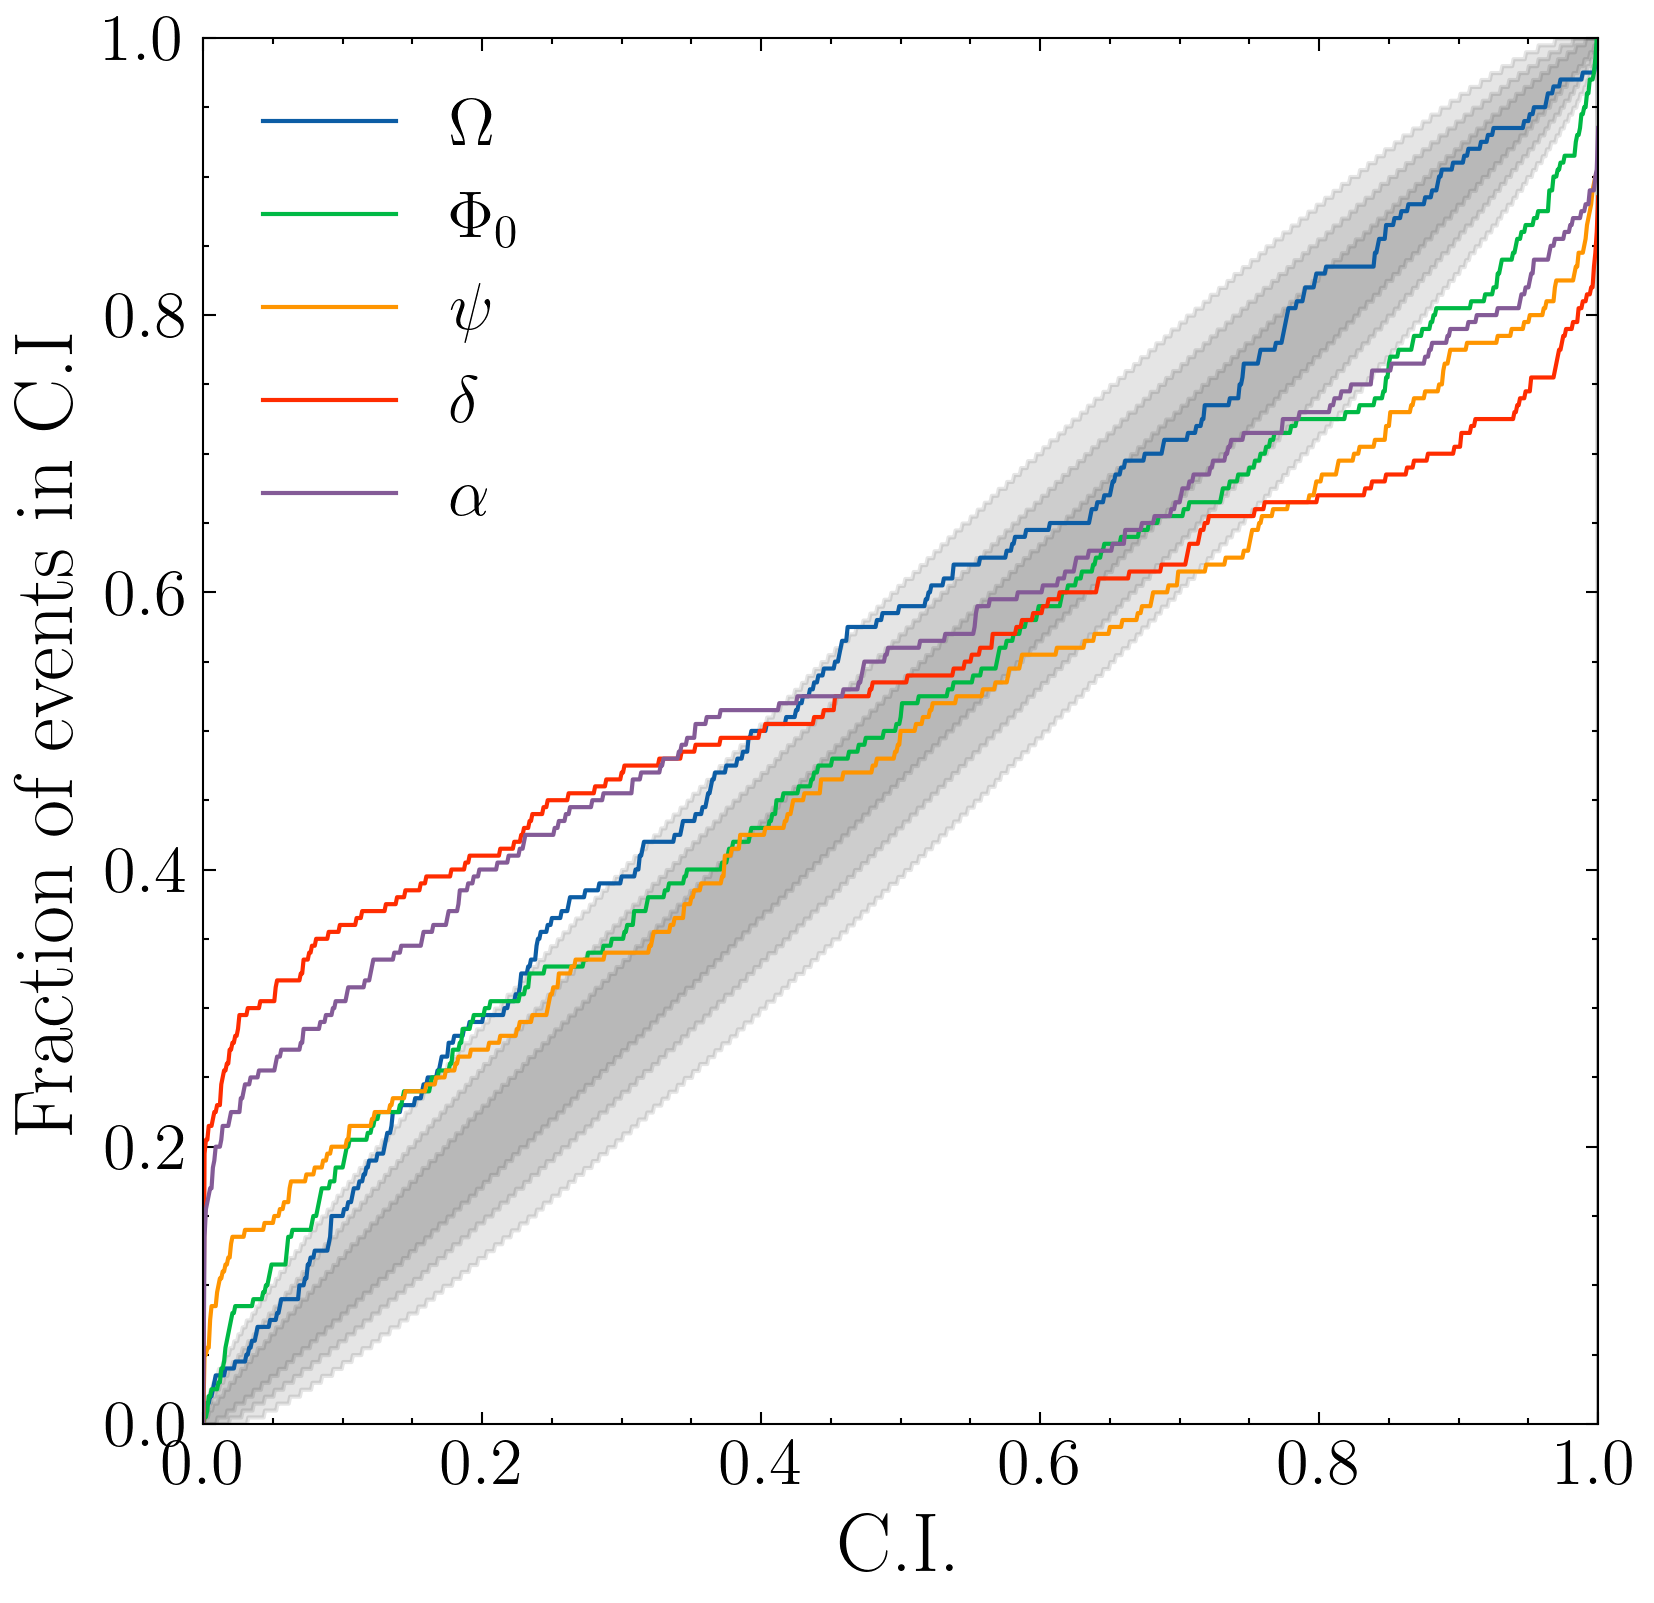
\includegraphics[width=\columnwidth]{images/pp_plot_new}
	\caption{PP plot for 200 simulated GW sources for a subset of parameters of $\boldsymbol{\theta}_{\rm gw}$, randomly drawn from the prior distributions of Table \ref{tab:parameters_and_priors}. Each coloured line corresponds to a different parameter of $\boldsymbol{\theta}_{\rm gw}$. The parameters $h_0$ and $\iota$ are fixed at $5 \times 10^{-15}$ and 1.0 rad respectively in order to maintain an approximately constant SNR. The grey shaded contours labels the $1,2,3$-$\sigma$ confidence intervals. Well estimated posteriors should fall along the diagonal $y=x$. $\Omega$ is generally well-estimated but many other parameters show evidence of being over-constrained due to a modelling bias. }
	\label{fig:parameter_space}
\end{figure}
We have so far focussed on a single representative system, summarised in Table \ref{tab:parameters_and_priors}. \DIFdelbegin \DIFdel{It is also important to }\DIFdelend \DIFaddbegin \DIFadd{In this section we }\DIFaddend test the method in different regions of the parameter space\DIFdelbegin \DIFdel{. To this end we }\DIFdelend \DIFaddbegin \DIFadd{, varying the source parameters through astrophysically relevant ranges. }\newline 


\DIFadd{We }\DIFaddend consider 200 injections for different sets of parameter values where we fix $h_0 = 5 \times 10^{-15}$, $\iota =1.0$ and draw the remaining five parameters of $\boldsymbol{\theta}_{\rm gw}$ from the prior distributions described in Table \ref{tab:parameters_and_priors}. We fix $h_0$ and $\iota$ in order to maintain an approximately constant SNR across the parameter space. For each simulated injection we can then attempt to recover the posterior distributions for each parameter. To summarise the results across the parameter space we use a parameter-parameter (PP) plot \citep{doi:10.1198/106186006X136976}. A PP plot describes the fraction of the total number of injected parameters which are included within a given credible interval of the estimated posterior with respect to the credible interval itself. In the ideal case the PP plot should be a diagonal line, indicating that $x$-percentage of the simulated injections fall within the $x$-percentage credible interval. The results are shown in Figure \ref{fig:parameter_space}. The shaded grey contours enclose the $1\sigma$, $2\sigma$, and $3\sigma$ significance levels, given 200 injections. We can see that only $\Omega$ falls within the $3\sigma$ shaded region. The other parameters deviate from the $y=x$ diagonal. The effect is most pronounced for $\alpha$ and $\delta$ with more modest deviations for $\psi$ and $\Phi_0$. The shape of the graph indicates that the posteriors for these parameters are over-constrained; there are fewer injections contained within high value credible intervals than would be expected statistically, and there are more injections contained within the low value credible intervals. This is an result of the bias that we observed in Section \ref{sec:multiple_noise}; the posteriors inferred for these parameters are generally confident, but are systematically biased away from the true injection values. This manifests in the PP plot as posteriors which are overly precise (narrow) to contain the injected value within the appropriate credible interval. An in-depth discussion on the origin of this bias is given in Section \ref{sec:bias}. 


\DIFdelbegin \subsection{\DIFdel{Identifiability and bias}} %DIFAUXCMD
\addtocounter{subsection}{-1}%DIFAUXCMD
\DIFdelend \DIFaddbegin \section{\DIFadd{Identifiability and bias}} \DIFaddend \label{sec:bias_and_identifiability}
There are two underlying issues in the preceding tests that we now explore in more detail. The first relates to parameter identifiability, i.e. can we uniquely identify the parameters of the model given the data and the model structure? \DIFaddbegin \DIFadd{This question is explored in Section \ref{sec:identif}. }\DIFaddend The second relates to a bias in the parameter estimates that results from dropping the pulsar terms from the Kalman filter measurement equation as described in Section \ref{sec:parameter_estim}. \DIFaddbegin \DIFadd{This is the focus of Section \ref{sec:bias}. }\DIFaddend In order to elucidate these questions without confusion from the measurement noise, we now work in the high SNR regime and set $h_0 = 10^{-12}$ (c.f. Figure \ref{fig:bayes}) for our representative example system (Table \ref{tab:parameters_and_priors}). \footnote{\tiny \textcolor{red}{TK: This discussion on bias and identifiability is perhaps less relevant than it was when our representative example had a 'high' strain ($10^{-12}$). However it IS still a feature/bug of our approach and I think it is worth discussing in the main body rather than relegating to an appendix. Opinions welcome...} \normalsize}

\DIFdelbegin \subsubsection{\DIFdel{Identifiability}}
%DIFAUXCMD
\addtocounter{subsubsection}{-1}%DIFAUXCMD
\DIFdelend \DIFaddbegin \subsection{\DIFadd{Identifiability}}\label{sec:identif}
\DIFaddend \begin{figure}
	\centering
	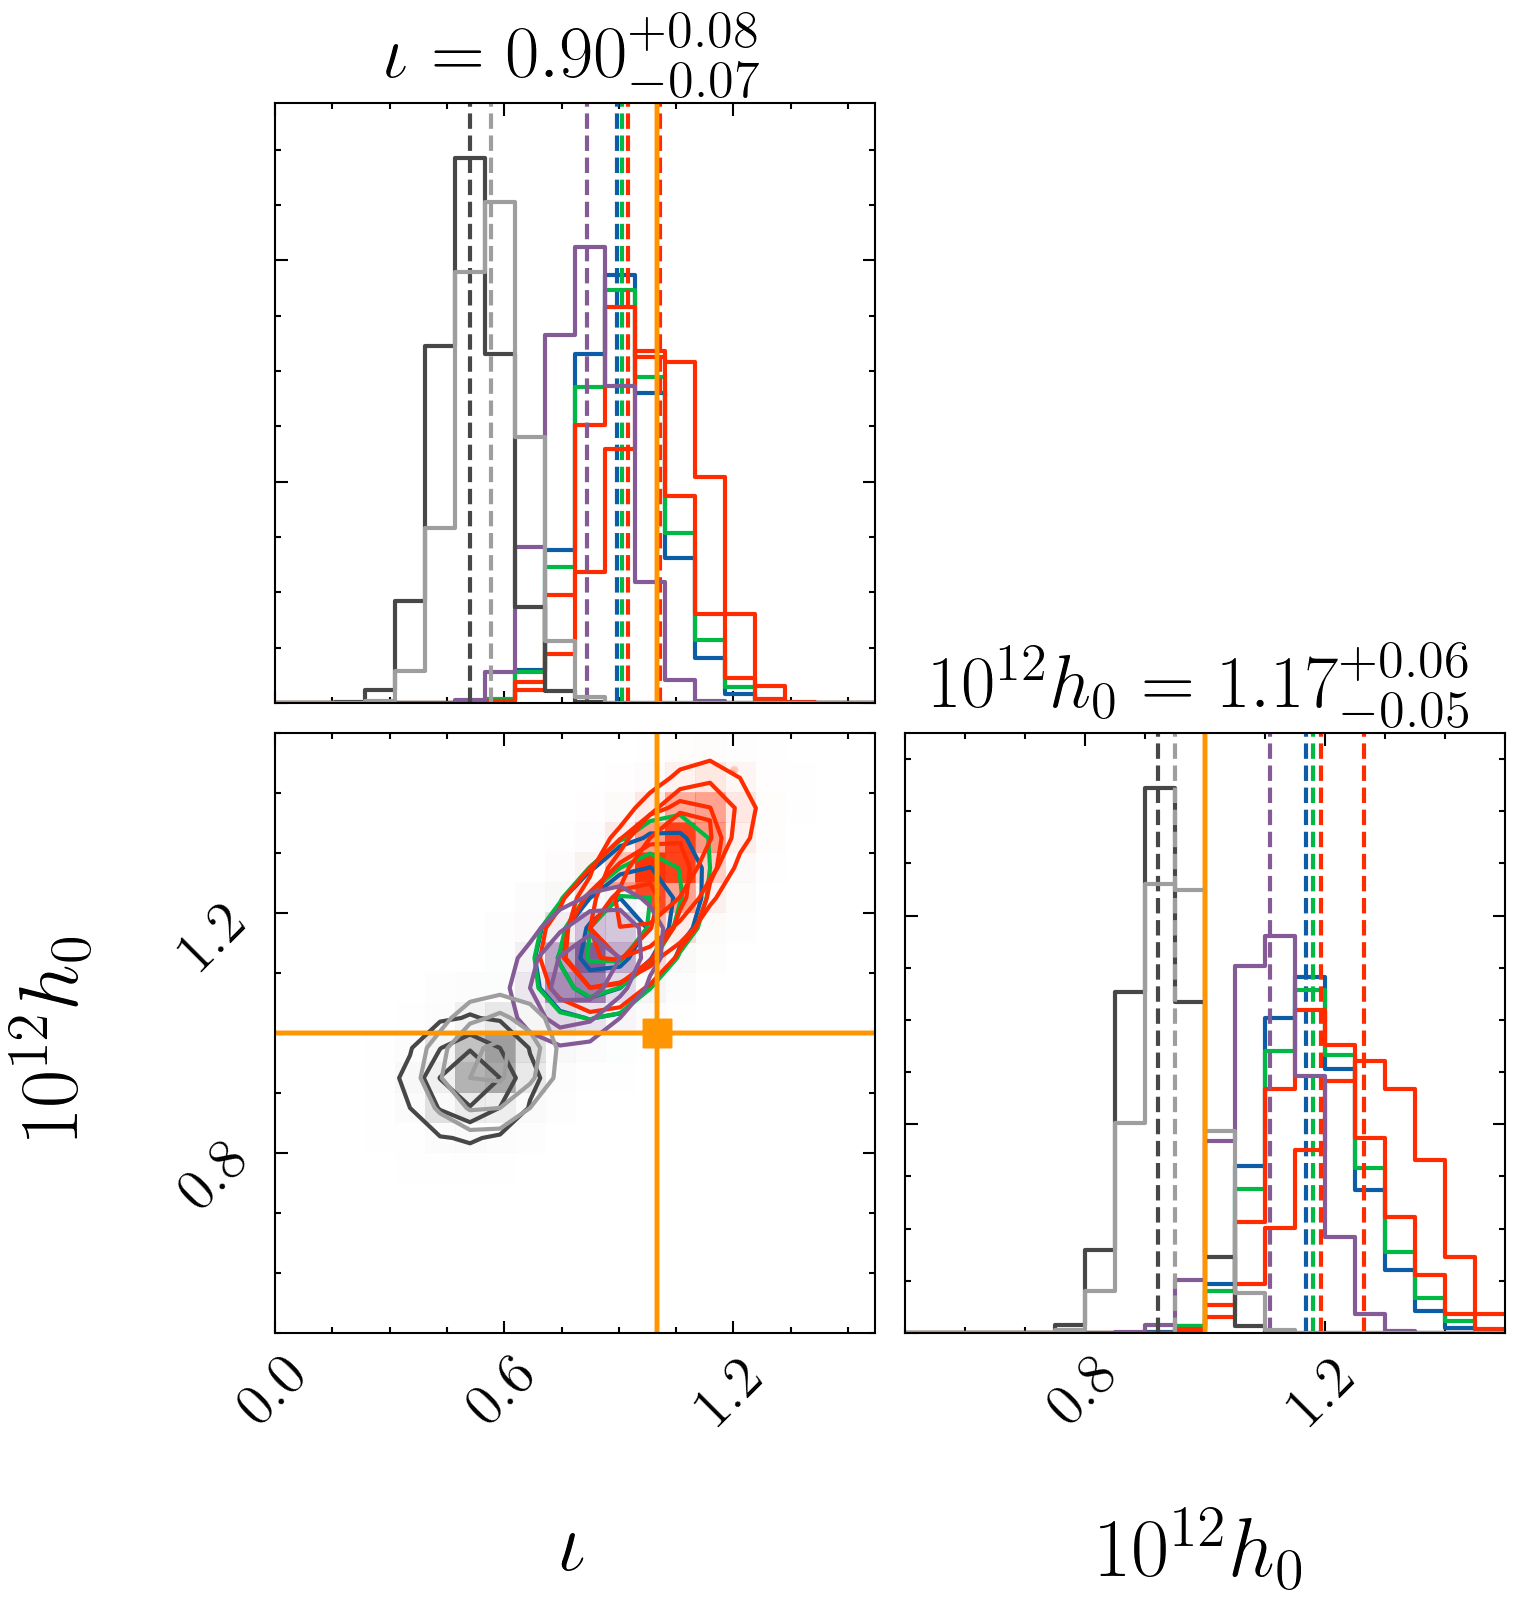
\includegraphics[width=\columnwidth]{images/stacked_GW_plot_iota_h}
	\caption{Posterior probability distributions for the representative system described in Table \ref{tab:parameters_and_priors} over nine noise realisations for the GW source parameters $\iota$ and $h_0$ in the high SNR regime ($h_0 = 10^{-12}$). Unlike the other parameters of  $\boldsymbol{\theta}_{\rm gw}$, the one-dimensional posteriors for $\iota$ and $h_0$ do not strongly overlap. A correlation between  $\iota$ and $h_0$ is evident.}
	\label{fig:just_iota_h}
\end{figure}
\begin{figure}
	\centering
	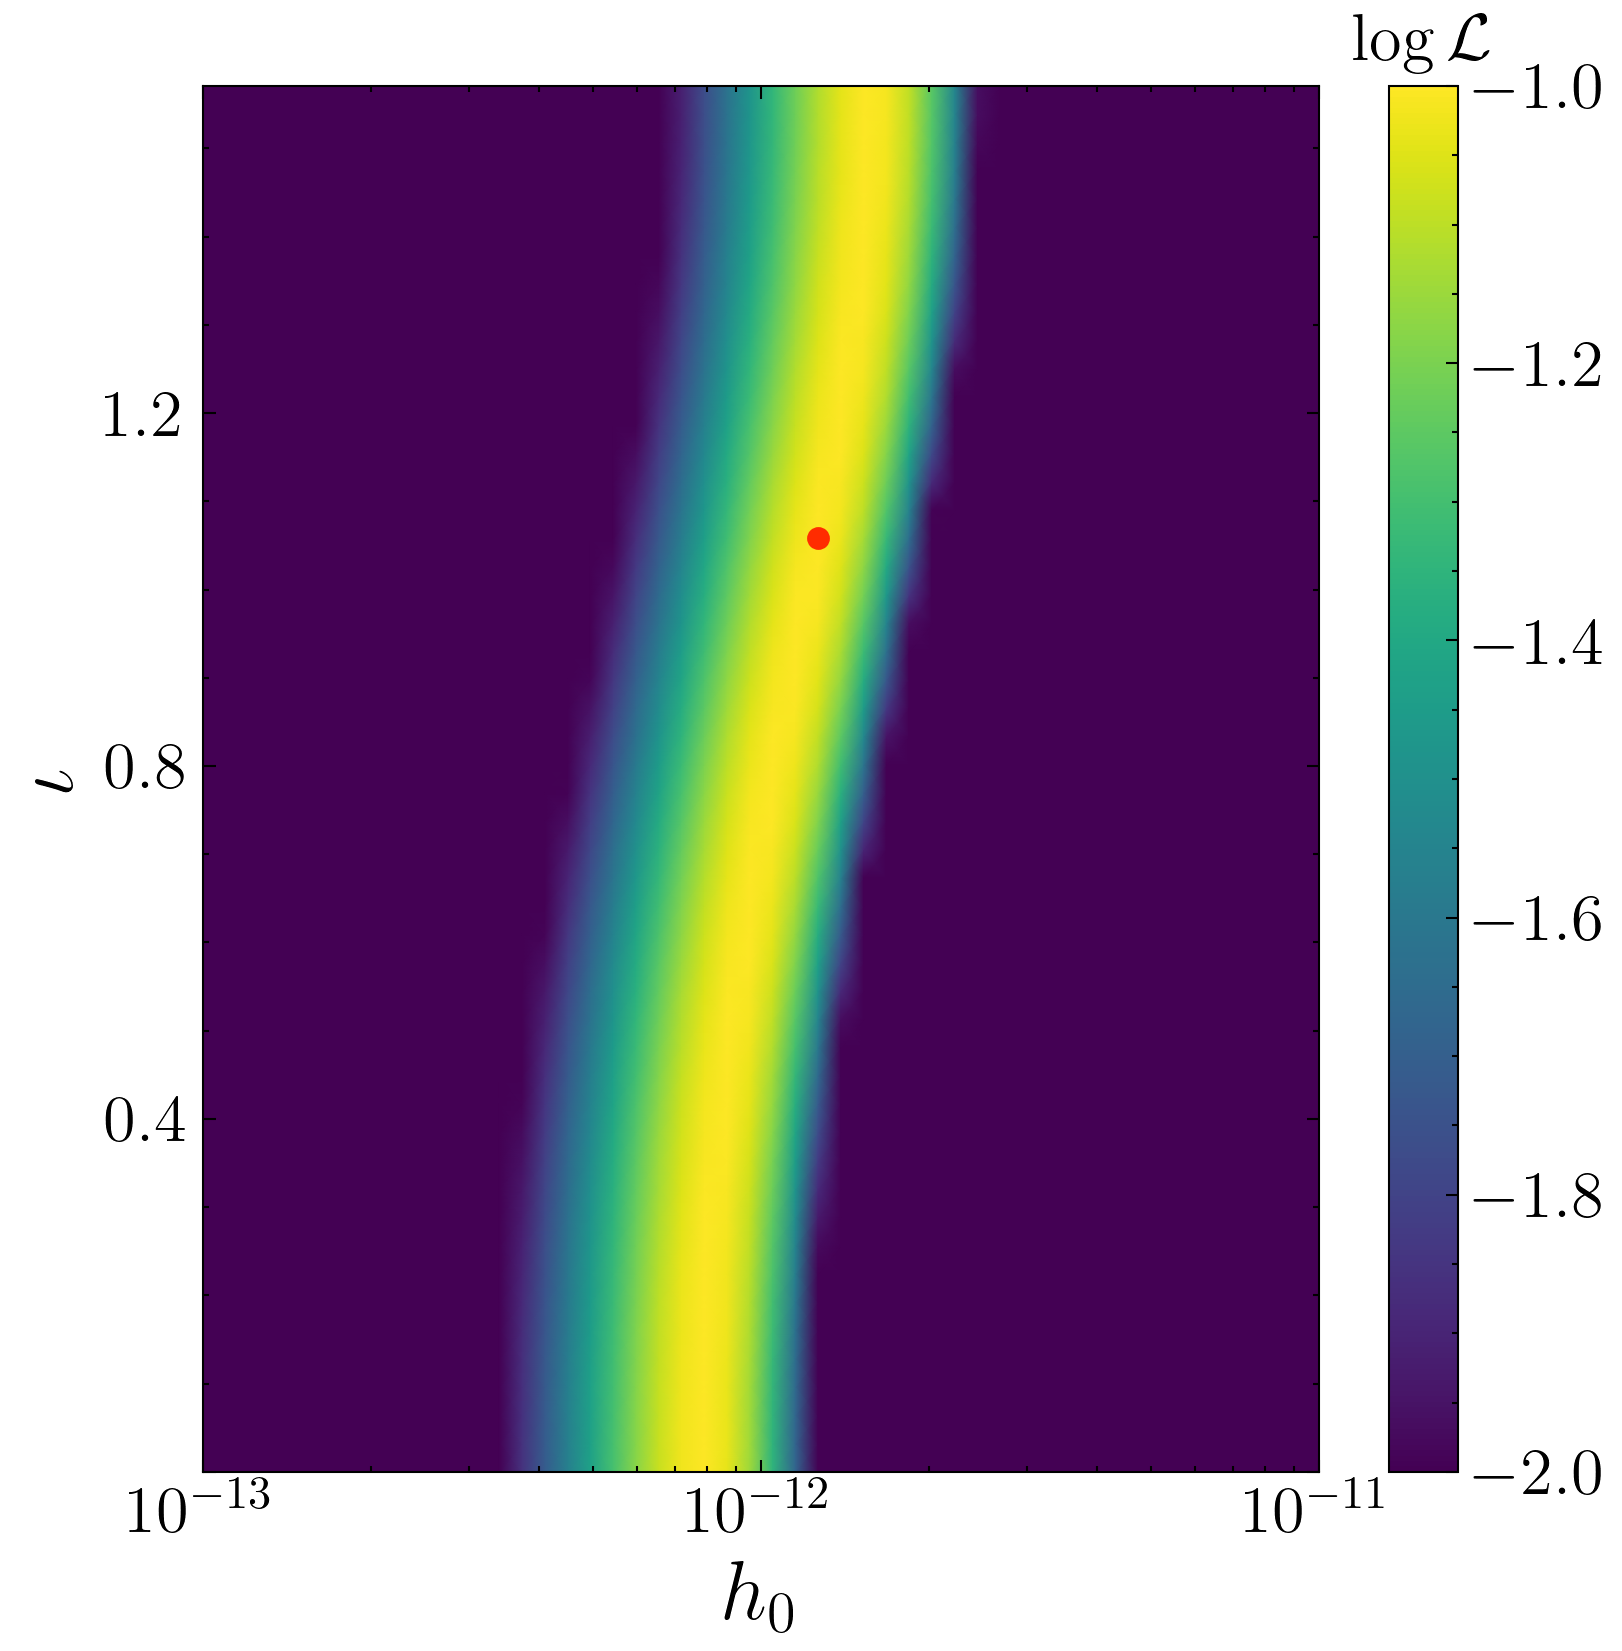
\includegraphics[width=\columnwidth]{images/likelihood_surface}
	\caption{Likelihood $\log \mathcal{L}$ (Equation \ref{eq:likelihood}) surface across the $\iota - h_0$ parameter space for a single noise realisation. The red point labels the location of the likelihood maxima. The likelihood surface has been normalised with respect to the absolute value of the maxima. A strong likelihood ridge is evident in the parameter space where the Kalman filter produces similar likelihood values, making it difficult for sampling algorithms to converge to a consistent value.}
	\label{fig:likelihood_surface}
\end{figure}
In Figure \ref{fig:just_iota_h} we plot the estimated one-dimensional posteriors for $\iota$ and $h_0$ for our high-SNR representative system, over nine noise realisations. 
\DIFaddbegin \DIFadd{The figure is entirely analogous to Figure \ref{fig:corner_plot_2}, but just for $\iota$ and $h_0$ rather than all members of $\boldsymbol{\theta}_{\rm gw}$. }\DIFaddend In the case of high-SNR we might expect \textit{a priori} that our estimates would be increasingly accurate over the low-SNR case, and that the method would converge robustly to similar posteriors irrespective of the noise realisation (i.e. $W_1 \to 0$). This is generally true for the majority of the component parameters of $\boldsymbol{\theta}_{\rm gw}$; the estimated posteriors across noise realisations are largely indistinguishable. However for $\iota$ and $h_0$ this is not the case. Instead the inferred one-dimensional posteriors do not broadly overlap and are not consistent across different noise realisations. Specifically across $10^3$ noise realisations the median WD for $\iota$ is $W_{1, \rm median}=0.24$ rad and for $h_0$ is  $W_{1, \rm median}=1.6 \times 10^{-13}$. For $\iota$, $W_{1,\rm median}$ is greater than the value inferred in the low SNR case ($=0.14$, Table \ref{tab:Wasserstein}), whilst for $h_0$ $W_{1,\rm median}$ is also greater as a proportion of the scale set by the strain amplitude. This is in contrast to $W_{1,\rm median}$ inferred for the other parameters of $\boldsymbol{\theta}_{\rm gw}$ in the high-SNR regime where as SNR increases, $W_1$ decreases; e.g. for $\Phi_0$, $W_{1, \rm median} = 4.5 \times 10^{-3}$ rad. \newline 

This issue of inferring very different posteriors depending on the particular realisation of the noise is due to these parameters being only weakly-identifiable. Identifiability refers to whether it is theoretically possible to infer unique parameter values of the model, given the measured data and the model structure \citep{e5be7c83a0d24500826f6e1b414d1733}. Sources of non-identifiability are generally categorised as either ``structural", arising from the structure of the model, or ``practical", arising from insufficient data or measurement errors \citep{GUILLAUME2019418}. Regarding $\iota$ and $h_0$, we are concerned with structural identifiability. Indeed, one might initially suspect that $\iota$ and $h_0$ could have structural identifiability issues; from Equations \eqref{eq:hphx} and \eqref{eq:hphx2} we can see that there is a weak degeneracy between $\iota$ and $h$. For example, from Equation \eqref{eq:hphx2} it is not clear if a larger value of the cross polarisation strain $h_{\times}$ is due to the system having a larger strain amplitude $h_0$, or a different inclination $\iota$. This degeneracy is only broken by the relation for $h_{+}$, Equation \eqref{eq:hphx}. It can be shown (Appendix \ref{appendix_identifiability}) that $\iota$ and $h_0$ are in fact structurally identifiable, but with the caveat that they are only weakly-identifiable. That is to say the $\iota-h_0$ likelihood surface plateaus to a ridge with a small, non-zero gradient close to the maximum likelihood solution. This likelihood ridge is presented in Figure \ref{fig:likelihood_surface} for a particular noise realisation. Whilst a single, unique maxima exists (labelled by the red point in the figure), along the ridge in the parameter space the likelihood values are all very similar. Consequently it is difficult for the nested sampling algorithm to select a particular point in this plateau and instead effectively trades off accuracy in one parameter against accuracy in other, depending on the particular realisation of the noise. If during the inference we fix one of the parameters at its true value (i.e. set a delta function prior), taking a slice through the likelihood surface it is then possible to identify a particular point in the plateau and the posteriors for the different noise realisations overlap indistinguishably, i.e. $W_1 \to 0$. In the low-SNR case these parameters are also weakly identifiable, but the increased measurement noise increases the uncertainty which effectively ``washes out" \footnote{\tiny \textcolor{red}{TK: "washes out" may be too colloquial / unspecific, but I think it is intuitive...}\normalsize}the likelihood ridge, leading to a more concave likelihood surface. This enables consistent posteriors to be estimated for $\iota$ and $h$. In the case where we fix e.g $h_0$ at its true value to infer indistinguishable posteriors for $\iota$, all of the posteriors for $\iota$ are all strongly biased away from the injected value; the maximum a posteriori probability estimates underestimate the injected value by $\sim 0.34$ rad. This is a more definitive sign of the bias that was suggested at in Sections \ref{sec:parameter_estim} and \ref{sec:multiple_noise} and will be now be discussed further in Section \ref{sec:bias}. 
\DIFdelbegin \subsubsection{\DIFdel{Bias by dropping pulsar terms}}%DIFAUXCMD
\addtocounter{subsubsection}{-1}%DIFAUXCMD
\DIFdelend \DIFaddbegin \subsection{\DIFadd{Bias by dropping pulsar terms}}\DIFaddend \label{sec:bias}

\begin{figure*}
	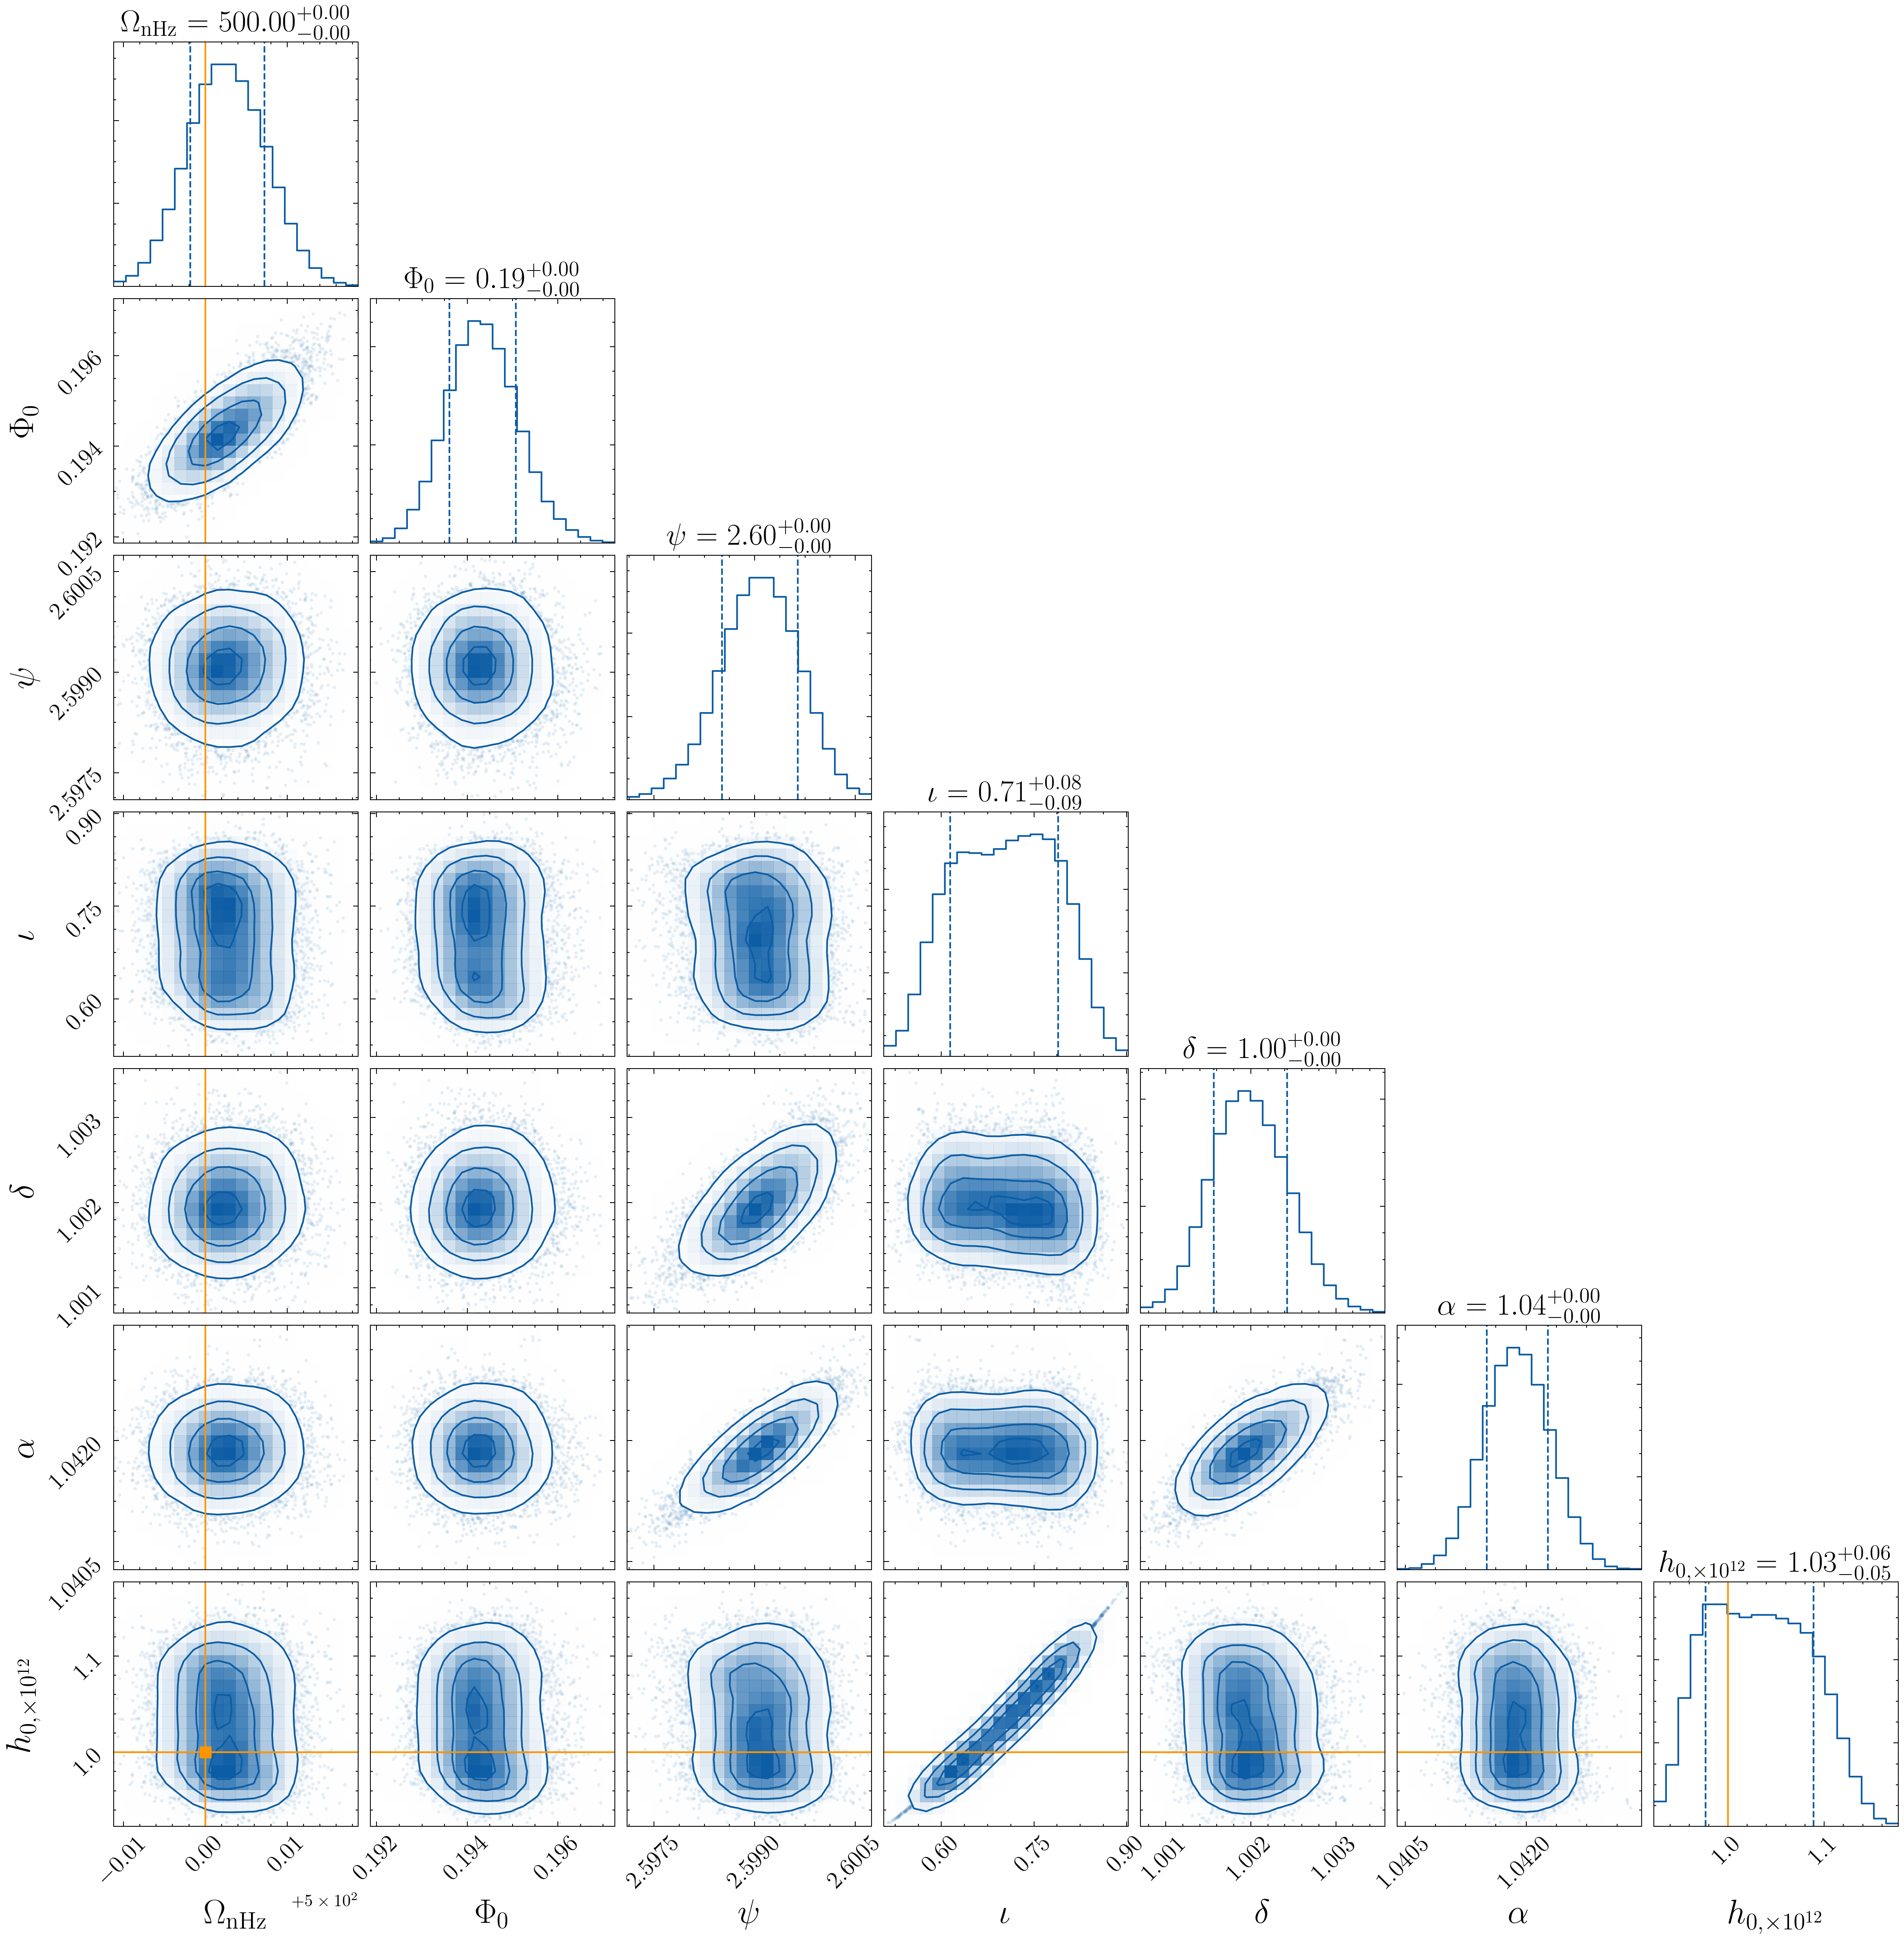
\includegraphics[width=\textwidth, height =\textwidth]{images/large_h_example}
	\caption{As Figure \ref{fig:corner_plot_1} but for the high-SNR system with $h_0 = 10^{-12}$. For the majority of parameters the injection value does not fall within the 90\% credible interval and is not visible over these scales. The estimated posteriors are biased away from the injected value due to the dropping of the pulsar terms. Note that the scale of the $x$-axes are generally highly constrained compared to Figure \ref{fig:corner_plot_1}.} 
	\label{fig:bias_for_large_h}
\end{figure*}

\begin{figure}
	\centering
	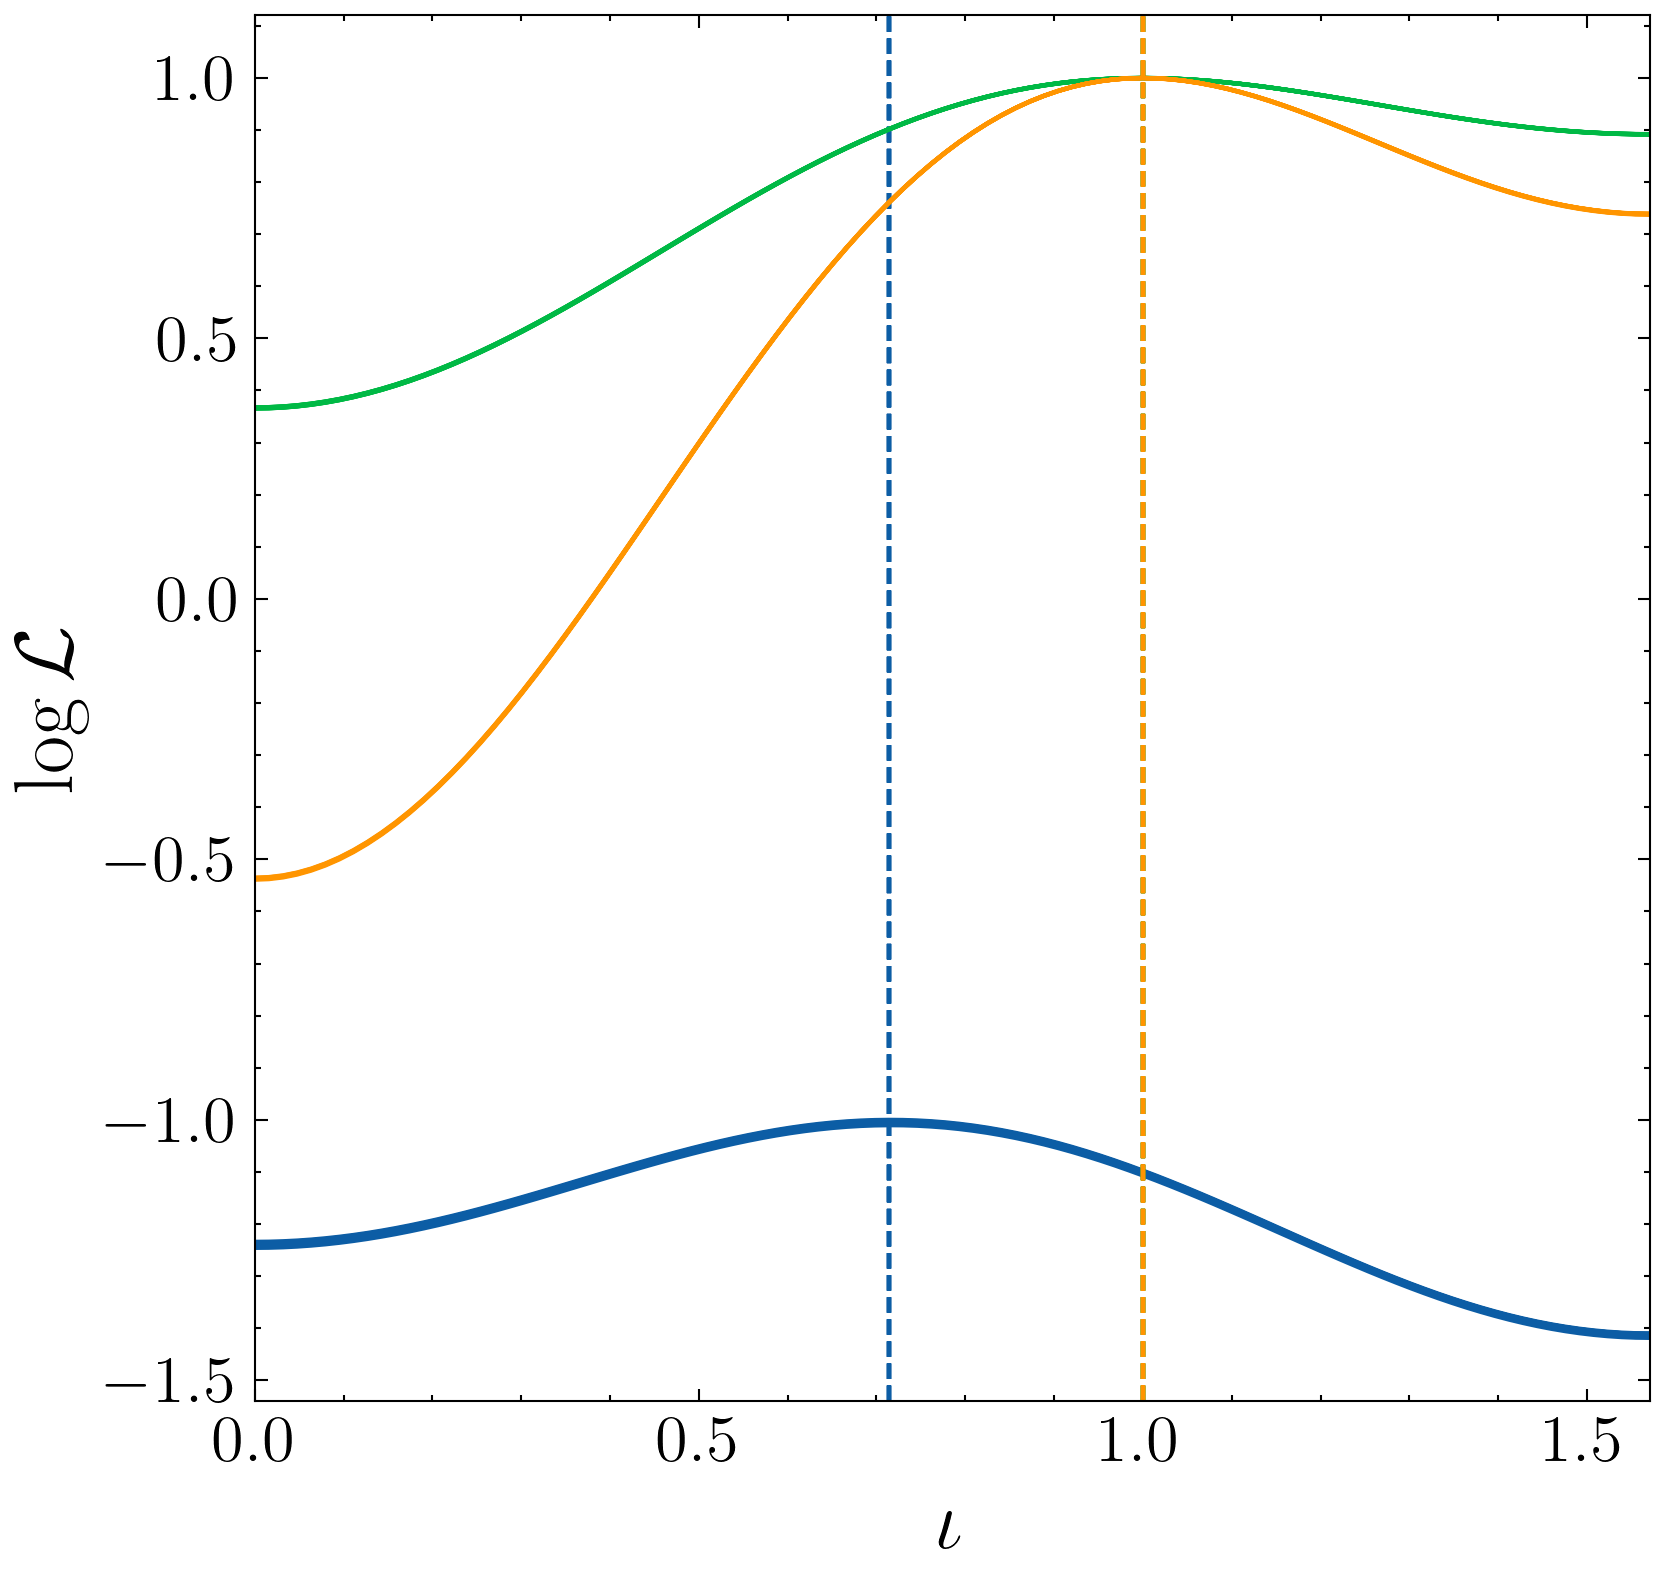
\includegraphics[width=\columnwidth]{images/likelihood_iota_new}
	\caption{Variation in the log likelihood returned by the Kalman filter using the Earth terms model (Equation \ref{eq:measuremen_earth}, blue line), the pulsar terms model (Equation \ref{eq:measurement}, orange line), and the Earth terms model for Earth terms only synthetic data (green line), with respect to the inclination $\iota$, over the prior space. All other parameters are fixed at their true injected value from Table \ref{tab:parameters_and_priors}. The coloured dashed vertical lines label the location of the likelihood maxima for their corresponding model; the green/orange dashed lines are overlaid on this scale. For the Earth-terms model the likelihood maxima does not coincide with the injected value ($\iota = 1.0$). For the pulsar-terms model the location of the maxima and injected value do coincide. 10 noise realisations are plotted for each situation but the solutions are completely overlaid on this scale.}
	\label{fig:likelihood_surface_iota}
\end{figure}
Evident in the preceding discussion is the fact that for some of the $\boldsymbol{\theta}_{\rm gw}$ parameters the inferred value (e.g. the median of the one-dimensional marginalised posterior) is biased away from the true injection value. In Figure \ref{fig:bias_for_large_h} we show the resulting posteriors for $\boldsymbol{\theta}_{\rm gw}$, analogous to Figure \ref{fig:corner_plot_1}, but now for the high-SNR system with $h_0 = 10^{-12}$. We can see that for all parameters, with the exception of $\Omega$ and $h_0$, the injected value lies outside the 90\% credible interval, to the extent that it is not visible on the scales over which we have plotted the posteriors. This effect is most severe for $\iota$ with a bias of $\sim 0.3$ rad but is also present to a lesser extent in other static parameters such as $\delta,\alpha$ and $\psi$, and additionally to an even smaller extent in $\Phi_0$. Similar results are obtained for other noise realisations. Whilst $h_0$ does not exhibit any noticeable bias for this particular noise realisation, in general across multiple noise realisations it does exhibit a correlated bias with $\iota$. In this Section we demonstrate how this bias results from the dropping of the pulsar terms described in Section \ref{sec:parameter_estim}. \newline 


In Figure \ref{fig:likelihood_surface_iota} we plot the variation in the log-likelihood returned by the Kalman filter, Equation \eqref{eq:likelihood}, as we vary $\iota$ across the prior space, holding all other parameters constant at the true injected value of the representative example system, Table \ref{tab:parameters_and_priors}. We do this for 10 separate realisations of the system noise. We consider three separate situations: \textit{(i)} The solid blue line is the likelihood curve with just the Earth-terms included (i.e. using Equation \ref{eq:measuremen_earth} in the Kalman filter), \textit{(ii)} the solid orange line is the likelihood curve with the additional pulsar terms included (i.e. using Equation \ref{eq:measurement}), \textit{(iii)} the solid green line is the solution where we drop the pulsar terms from both the synthetic data and the measurement equation. We have not used nested sampling for situations \textit{(ii)} or \textit{(iii)} in this work. However, we are able to run the Kalman filter either using the pulsar terms in the model or else dropping them from the synthetic data consider how the resulting likelihood varies for different parameter values. The dashed lines show the location of the likelihood maxima for each of the likelihood solutions; finding the location of the maxima across all static parameters is effectively the goal of any likelihood based inference method, such as nested sampling. \newline  

The key observation from Figure \ref{fig:likelihood_surface_iota} is that for the Earth-terms only solution the location of the likelihood optima and the location of the injected value are not the same. Consequently Bayesian likelihood inference techniques settle in optima that do not necessarily align with the true injection value. This is the origin of the bias in the one-dimensional marginalised posteriors that we observe.  For the Earth-terms solution the optima of the likelihood curve lies around $\iota \sim 0.7$ radians, whereas the injected value was $\iota = 1.0$ radians. This optima is comparable to the median of the posterior inferred for $\iota$ in Figure \ref{fig:bias_for_large_h}. \newline 

In contrast to the Earth-terms solution, for the pulsar-terms solution the optima of the likelihood curve now aligns with the true injected value. The corollary is also true; if we drop the pulsar terms from the synthetic data and use the Earth terms equation for inference then the optima is also correctly located. This evidences that it is the effect of dropping the pulsar terms from the measurement equation which causes this bias in the inferred posteriors. Similar results are observed for the other parameters which exhibit a bias in the nested sampling inference. \newline 

Why does dropping the pulsar terms bias these parameters in particular, whilst leaving others unaffected? For instance, why is the bias induced in $\iota$ so strong, whereas $\psi$ shows only a weak bias and  $\Omega$ shows no bias at all? When we generate synthetic data including the pulsar term, the state frequency of an individual pulsar $f_{\rm p}$ is effective modulated by the interference of two equal-amplitude, phase shifted waves (c.f. Equation \ref{eq:measurement}). Explicitly, we have the ``Earth-terms wave"	 with a general form $y_{\rm Earth} = A \cos \xi$ for amplitude $A$ and phase $\xi$ and the ``pulsar-terms wave" with a general form $y_{\rm pulsar} = A \cos (\xi + \kappa)$ for phase offset $\kappa$. The net interference wave that modulates $f_{\rm p}$ is 
\begin{eqnarray}
	y_{\rm Earth} - y_{\rm pulsar} = 2 A \sin \left(\frac{\kappa}{2}\right) \sin \left(\xi + \frac{\kappa}{2}\right) \ .
\end{eqnarray}
The additional modulations from $y_{\rm pulsar}$ influence the amplitude of the resulting interference wave, but do not affect its frequency. When we model this data using the Kalman filter without the pulsar terms, the additional amplitude modulations from $y_{\rm pulsar}$ must be described by the single wave model, $y_{\rm Earth}$. As a result the $y_{\rm Earth}$ model must try to compensate for these amplitude modulations by adjusting the parameters which govern the amplitude of the single wave. Consequently the parameters which are most affected are those which determine the amplitude of the GW. Terms which influence the amplitude strongly, such as $h_0$ and $\iota$, are strongly affected and exhibit a strong bias. Terms which influence the amplitude weakly such as $\psi$ exhibit a weaker bias. The wave amplitude is independent of the frequency and so $\Omega$ exhibits no bias. Since a shift in phase affects the instantaneous amplitude of the wave, $\Phi_0$ also exhibits a small bias, despite $A$ not being a function of $\Phi_0$. This hierarchy of biases for each parameter is also what we observe in Figure \ref{fig:parameter_space}, where $\alpha$ and $\delta$ are strongly over-constrained whilst $\Omega$ is well-estimated. \newline  

In order to ascertain how important the bias is for PTA continuous wave searches requires a thorough exploration of the astrophysical parameter space which we do not carry out in this work. The magnitude of the bias will vary for different points in the parameter space, as well as for different PTA configurations. If the bias is sufficiently modest then for quiet continuous wave sources with low SNR the uncertainty in the one-dimensional marginalised posterior may dominate and the bias may not be important for searches. This is what we observe for our synthetic data (e.g. Figure \ref{fig:corner_plot_2}); the decreased SNR manifests as a broader marginalised posterior which generally overwhelms the shift due to the bias. Conversely if the bias is sufficiently strong, or the source sufficiently loud with low uncertainties, then the bias may come to systematically affect the inferred parameters. \newline  

We have shown in this section how the dropping of the pulsar terms results in a bias in the inferred parameters, not just in the sky localisation parameters  \citep[e.g.][]{Zhupulsarterms,Chen2022} but additionally all parameters which influence the wave amplitude. Whilst the bias is generally small and does not prevent the recovery of accurate posteriors for our example system, it is present and may need to be accounted for for analysis in other parts of the parameter space. This bias is not particular to our method but a shared feature across likelihood based methods that do not include the pulsar terms in the inference model. The inclusion of the pulsar terms in the methods presented in this work in order to alleviate the bias will be a key goal of a future work. 


\section{Discussion}\DIFaddbegin \label{sec:discussion}
\DIFaddend We have shown how our complementary approach to PTA data analysis using a Kalman filter can successfully recover the underlying parameters of the model and calculate Bayes factors in order to perform Bayesian model selection. There are a number of potential extensions of this work which we now discuss.  \newline 

The natural first extension is to implement the method whilst retaining the pulsar terms of Equation \ref{eq:measurement}. Whilst PTA searches commonly drop the pulsar terms as standard practice, we have shown that this leads to biases in the inferred one-dimensional marginalized posteriors for the model parameters. Biases in sky localisation for synthetic datasets as a result of dropping the pulsar terms are also observed by \cite{Zhupulsarterms} and \cite{Chen2022}. Alternatively, if the method continues to be used with solely the Earth terms then it would be highly desirable to make systematic, quantitative estimates of the incurred biases in the model parameters across an astrophysically representative parameter space. \newline 

We have considered only a specific configuration of pulsars composing our synthetic PTA - the same pulsars that make up the 12.5-year NANOGrav (Section \ref{sec:synt_pta}). Whilst our method is generally independent of the specific choice of pulsars, it would be of interest to compare the performance of the method using different pulsars configurations and different PTAs such as PPTA and the EPTA. Indeed, since adding pulsars to PTAs increases the computational demands of the data analysis it may be advantageous to optimally select a subset of the total available pulsars which may be able to provide comparable performance to a larger PTA  \citep{2023MNRAS.518.1802S}.  \newline 

Throughout this work we have assumed that all pulsars are observed at the same time, with a constant time sampling. In practice this assumption does not hold and different pulsars will be observed with different cadences at different times. Extending this method to non-constant time sampling is straightforward and the performance of the method should be evaluated in this regime. \newline 

We have taken our GW source to be monochromatic, i.e. $\Omega$ is a fixed parameter with no time dependence. Whilst this is an astronomically well-justified assumption (see discussion in Section \ref{sec:plane_gw}), and appropriate for this initial methods work, it would also be of interest to extend the state-space construction to enable the GW frequency to evolve in time. The GW source is monochromatic over the decadal PTA observation period, but the timescale set by the Earth-pulsar distance is comparable to the SMBHB evolution timescale \citep{Sesana2010}. For $\Delta f_{\rm gw} < 1 / T_{\rm obs}$ (see Equation \eqref{eq:f_evolution}) the GW source frequency evolution manifests as an incoherent source of noise in the pulsar terms, whilst for  $\Delta f_{\rm gw} > 1 / T_{\rm obs}$ the pulsar terms can affect the phase coherency of the Earth terms \citep{Perrodin2018}. Careful consideration of the evolution of the GW frequency will be important as we look to extend our method to include the pulsar terms in the inference model. \newline 


We have also assumed that there is only a single GW source that influences the received pulsar frequencies. However, it may be possible to resolve multiple continuous GW sources concurrently \citep{PhysRevD.85.044034}. Our method naturally extends to detecting multiple GW sources simultaneously; Equation \eqref{eq:measurement} is straightforwardly modified to become a linear superposition of multiple GWs. The stochastic background itself is the incoherent summation of many individual GW sources. It therefore stands to reason that it may be possible to extend this method to also search for a stochastic GW background, providing a complementary approach to detect the stochastic background without requiring a cross-correlation of the pulsar residuals to uncover the Hellings-Downs curve. \newline 


\textcolor{red}{TK: Lets also pre-empt reviewer and make it explicit why we are using frequencies rather than TOAs. Need to chat with group to get this clear in my head.}


%https://arxiv.org/pdf/2107.03047.pdf
\section{Conclusion}\DIFaddbegin \label{sec:conclusion}
\DIFaddend In this paper we demonstrate a new method for the detection and parameter estimation of GWs from individual, monochromatic SMBHBs. We track the evolution of the intrinsic pulsar timing noise explicitly via a state-space method, rather than subtracting the ensemble-averaged statistics. That is, we disentangle statistically the specific time-ordered realisation of the timing noise from the GW induced modulations. This enables the inference of GW parameters conditioned on the specific observed realisation of the noisy data. We introduce the Kalman filter in order to track the intrinsic state evolution of the pulsar and combine this with a Bayesian sampling framework to estimate the posterior distributions of each parameter of the system, as well as the associated evidence (marginalised likelihood) of the model. We test our method on synthetic data. We initially focus on a single, astrophysically representative, SMBHB GW source detected with the 12.5-year NANOGrav pulsars observed over a 10 year timespan. The parameters of the model are accurately recovered and the minimal detectable strain is estimated to be $h_0 \sim 4 \times 10^{-15}$ for $\iota=1.0$ rad. The method is then further tested over 1000 noise realisations. Consistent posterior estimates of the parameters are obtained for the majority of noise realisations, with the median Wasserstein distance across all noise realisations $W_{1, \rm median}$ generally small compared to the prior space ($\lesssim 3 \%$). For a minority of noise realisations the nested sampler converges poorly and settles into a local likelihood optima for the posteriors estimates of $\psi$ and $\alpha$. This problem can be solved in general by increasing the number of live points $n_{\rm live}$ used by the sampler. Exploration of a broader parameter space via 200 randomly sampled parameter vectors highlights biases in some parameters as a result of dropping the pulsar terms from the inference model. The cause of these biases is examined for the case of high SNR, along with the structural weak-identifiability between $\iota$ and $h_0$. The extension of this method to include the pulsar term is a key challenge for a future work.

 

 
\appendix

\section{Kalman recursion equations} \label{sec:kalman}
The linear Kalman filter \DIFdelbegin \DIFdel{operate }\DIFdelend \DIFaddbegin \DIFadd{operates }\DIFaddend on temporally discrete, noisy measurements $\boldsymbol{Y}_k$\DIFaddbegin \DIFadd{, }\DIFaddend which are related to a set of unobservable discrete system states $\boldsymbol{X}_k$\DIFaddbegin \DIFadd{, }\DIFaddend via a linear transformation:
\begin{equation}
	\boldsymbol{Y}_k = \boldsymbol{H}_k \boldsymbol{X}_k + \boldsymbol{v}_k \DIFaddbegin \DIFadd{\ ,}\DIFaddend \label{eq:kalman1}
\end{equation}
where $\boldsymbol{H}_k$ is the measurement matrix or observation model, $\boldsymbol{v}_k$ is a zero-mean Gaussian measurement noise\DIFdelbegin \DIFdel{with covariance $\boldsymbol{R}_k$}\DIFdelend , \DIFaddbegin \DIFadd{$\mathcal{N} \sim (0,\boldsymbol{R}_k)$ with covariance, }\DIFaddend and the subscript $k$ labels the time-step. The Kalman filter takes the underlying states to evolve according to
\begin{equation}
	\boldsymbol{X}_k = \boldsymbol{F}_k \boldsymbol{X}_{k-1} + \boldsymbol{G}_k \boldsymbol{u}_k + \boldsymbol{w}_k \DIFaddbegin \DIFadd{\ , }\DIFaddend \label{eq:kalman2}
\end{equation}
where $\boldsymbol{F}$ is the system dynamics matrix, $\boldsymbol{G}$ the \DIFdelbegin \DIFdel{input or }\DIFdelend control matrix. \DIFaddbegin \DIFadd{$\boldsymbol{u}$ the control vector, }\DIFaddend and $\boldsymbol{w}_k$ is a zero-mean Gaussian process noise\DIFdelbegin \DIFdel{with covariance $\boldsymbol{Q}_k$}\DIFdelend \DIFaddbegin \DIFadd{, $\mathcal{N} \sim (0,\boldsymbol{Q}_k)$}\DIFaddend . \newline 

The Kalman filter is a recursive estimator with two distinct stages; a ``predict" stage \DIFdelbegin \DIFdel{where the state at the current time-step is predicted based on the state at the previous time-step, }\DIFdelend and an ``update" stage\DIFdelbegin \DIFdel{where the predicted state estimate is refined based on the measurement at that time-step}\DIFdelend . The predict stage \DIFdelbegin \DIFdel{updates }\DIFdelend \DIFaddbegin \DIFadd{predicts }\DIFaddend the estimate of the state \DIFdelbegin \DIFdel{$\hat{\boldsymbol{X}}_{k|k-1}$ and the associated covariance $\hat{\boldsymbol{P}}_{k|k-1}$where the subscript notation ${k|k-1}$ denotes an estimate }\DIFdelend at discrete step $k$, given \DIFdelbegin \DIFdel{measurements }\DIFdelend \DIFaddbegin \DIFadd{the state estimates }\DIFaddend from step $k-1$\DIFdelbegin \DIFdel{and earlier. The }\DIFdelend \DIFaddbegin \DIFadd{. Specifically, the }\DIFaddend predict step proceeds as,
\begin{equation}
	\hat{\boldsymbol{X}}_{k|k-1} =  \boldsymbol{F}_k \hat{\boldsymbol{X}}_{k-1|k-1} + \boldsymbol{G}_k \boldsymbol{u}_k
\end{equation}
\begin{equation}
	\hat{\boldsymbol{P}}_{k|k-1} =  \boldsymbol{F}_k \hat{\boldsymbol{P}}_{k-1|k-1} \boldsymbol{F}_k^\intercal + \boldsymbol{Q}_k 
\end{equation}
\DIFdelbegin \DIFdel{The update step then uses the }\DIFdelend \DIFaddbegin \DIFadd{Note that the predict stage is independent of the measurements. The }\DIFaddend measurement $\boldsymbol{Y}_k$ \DIFdelbegin \DIFdel{to update $\hat{\boldsymbol{X}}_{k|k}$  and $\hat{\boldsymbol{P}}_{k|k}$ as ,
}\DIFdelend \DIFaddbegin \DIFadd{is included to update the prediction during the update stage as follows:
}\DIFaddend \begin{equation}
	\boldsymbol{\epsilon}_{k} = \boldsymbol{Y}_k - \boldsymbol{H}_k \hat{\boldsymbol{X}}_{k|k-1}
\end{equation} 
\begin{equation}
	\boldsymbol{S}_k = \boldsymbol{H}_k \hat{\boldsymbol{P}}_{k|k-1} \boldsymbol{H}_k^\intercal + \boldsymbol{R}_k
\end{equation}
\begin{equation}
	\boldsymbol{K}_k = \hat{\boldsymbol{P}}_{k|k-1} \boldsymbol{H}_k^\intercal \boldsymbol{S}_k^{-1} \label{eq:kalman gain}
\end{equation}
\begin{equation}
	\hat{\boldsymbol{X}}_{k|k} =\hat{\boldsymbol{X}}_{k|k-1} +\boldsymbol{K}_k  \boldsymbol{\epsilon}_{k}  \DIFaddbegin \label{eq:kalmangainupdate}
\DIFaddend \end{equation}
\begin{equation}
		\hat{\boldsymbol{P}}_{k|k} = \left( \boldsymbol{I} - \boldsymbol{K}_k \boldsymbol{H}_k \right) 	\hat{\boldsymbol{P}}_{k|k-1}
\end{equation}
Equation \eqref{eq:kalman gain} defines the ``Kalman gain" $\boldsymbol{K}_k$ which \DIFdelbegin \DIFdel{yields the minimal mean square }\DIFdelend \DIFaddbegin \DIFadd{is defined so as to minimise the mean squared }\DIFaddend error in the \DIFdelbegin \DIFdel{measurement post fit residual, $\boldsymbol{Y}_k - \boldsymbol{H}_k \hat{\boldsymbol{X}}_{k|k}$. }\DIFdelend \DIFaddbegin \DIFadd{state estimate, i.e.  $\boldsymbol{K}_k = \text{argmin} \left[ \boldsymbol{E}(\boldsymbol{X}_k - \hat{\boldsymbol{X}}_k) \right ]$. For a full review of the Kalman filter, including its derivation, we refer the reader to \mbox{%DIFAUXCMD
\cite{Gelb:1974} }\hskip0pt%DIFAUXCMD
and \mbox{%DIFAUXCMD
\cite{zarchan2000fundamentals}}\hskip0pt%DIFAUXCMD
. }\DIFaddend \newline 


We \DIFdelbegin \DIFdel{can map our }\DIFdelend \DIFaddbegin \DIFadd{map our continuous-time }\DIFaddend state-space model described in Section \ref{sec:model} onto the \DIFaddbegin \DIFadd{discrete-time }\DIFaddend Kalman filter structure of Equations  
\eqref{eq:kalman1}, \eqref{eq:kalman2} as follows. We identify $\boldsymbol{X}$ with a vector of length $N$ composed of the intrinsic pulsar frequency states, i.e 
\DIFdelbegin \DIFdel{$\boldsymbol{X} = \left(f_{\rm p}^{(1)}, f_{\rm p}^{(2)}, ..., f_{\rm p}^{(N)}\right)$. Similarly$\boldsymbol{Y} = \left(f_{\rm m}^{(1)}, f_{\rm m}^{(2)}, ..., f_{\rm m}^{(N)} \right)$. }\DIFdelend \DIFaddbegin \begin{equation}
	\DIFadd{\boldsymbol{X} = \left(f_{\rm p}^{(1)}, f_{\rm p}^{(2)}, ..., f_{\rm p}^{(N)}\right) \ .
}\end{equation}
\DIFadd{Similarly,  
}\begin{equation}
\DIFadd{\boldsymbol{Y} = \left(f_{\rm m}^{(1)}, f_{\rm m}^{(2)}, ..., f_{\rm m}^{(N)} \right)
}\end{equation}
\DIFaddend The states evolve according the continuous dynamical equation \DIFaddbegin \DIFadd{(c.f. Equation \eqref{eq:frequency_evolution})
}\DIFaddend \begin{equation}
	d \boldsymbol{X} = \boldsymbol{A} \boldsymbol{X} dt + \boldsymbol{C}(t) dt + \boldsymbol{\Sigma} d \boldsymbol{B}(t) \label{eq:kalmn2}
\end{equation}
where \DIFdelbegin \DIFdel{$\boldsymbol{A} = \text{diag} \left(\gamma^{(1)}, \gamma^{(2)}, ..., \gamma^{(N)}\right)$ is the state matrix
, $\boldsymbol{C} = \left(C^{(1)}, C^{(2)}, ..., C^{(N)}\right)$ the input or control matrix where $C^{(i)} =\gamma^{(i)} \left(f_{\rm em}^{(i)} (0) + \dot{f}_{\rm em}(0)^{(i)} t \right) +  \dot{f}_{\rm em}(0)^{(i)}$ and }\DIFdelend \DIFaddbegin \DIFadd{$\boldsymbol{A}$ is a diagonal $N \times N$ square matrix
}\begin{equation}
\DIFadd{\boldsymbol{A} = \text{diag} \left(\gamma^{(1)}, \gamma^{(2)}, ..., \gamma^{(N)}\right) \ ,
}\end{equation}
\DIFadd{and $\boldsymbol{C}(t)$ a time dependent vector with $n$-th component
}\begin{equation}
 \DIFadd{C^{(n)} =\gamma^{(n)} \left(f_{\rm em}^{(n)} (t_1) + \dot{f}_{\rm em}(t_1)^{(n)} t \right) +  \dot{f}_{\rm em}(t_1)^{(n)} \ .
}\end{equation}
\DIFadd{The $N \times N$ square matrix $\boldsymbol{\Sigma}$  governs the magnitude of the increments of Brownian motion (Wiener process) }\DIFaddend $d\boldsymbol{B}(t)$\DIFdelbegin \DIFdel{denotes a Wiener process with covariance matrix $\boldsymbol{\Sigma} = \text{diag} \left(\sigma^{(1)}, \sigma^{(2)}, ..., \sigma^{(N)}\right)$. Equation \ref{eq:kalmn2} is a Langevin equation (equivalently }\DIFdelend \DIFaddbegin \DIFadd{, where
}\begin{equation}
\DIFadd{\boldsymbol{\Sigma} = \text{diag} \left(\sigma^{(1)}, \sigma^{(2)}, ..., \sigma^{(N)}\right)
}\end{equation}
\newline 

\DIFadd{The evolution of the state is }\DIFaddend an Ornstein-Uhlenbeck process\DIFdelbegin \DIFdel{) }\DIFdelend \DIFaddbegin \DIFadd{, described by a Langevin equation, Equation \eqref{eq:kalmn2}, }\DIFaddend which has a general solution given by \citep{gardiner2009stochastic},
\begin{equation}
	\boldsymbol{X}(t) = e^{\boldsymbol{A} t} \boldsymbol{X}(0) + \int_0^t e^{\boldsymbol{A}(t-t')} \boldsymbol{C}(t') dt' + \int_0^t e^{\boldsymbol{A}(t-t')} \boldsymbol{\Sigma} d\boldsymbol{B}(t') \label{eq:gardenier}
\end{equation} 
From Equation \eqref{eq:gardenier} we can construct the discrete, recursive solution for $\boldsymbol{X}(t_k) = \boldsymbol{X}_k$ \DIFdelbegin \DIFdel{as }\DIFdelend \DIFaddbegin \DIFadd{in the form of }\DIFaddend Equation \eqref{eq:kalman2} where
\begin{equation}
\boldsymbol{F}_k = e^{\boldsymbol{A}\left( t_{k+1} - t_k \right)} 
\end{equation}
\begin{equation}
	\boldsymbol{G}_k = \int_{t_i}^{t_{i+1}}  e^{\boldsymbol{A}\left( t_{k+1} - t' \right)}  \boldsymbol{C}(t') dt' 
\end{equation}
\begin{equation}
	\boldsymbol{w}_k = \int_{t_k}^{t_{k+1}} e^{\boldsymbol{A}\left( t_{k+1} - t' \right)} \boldsymbol{\Sigma} d \boldsymbol{B}(t')
	\end{equation}
For our system, the state, control and process noise covariance matrices then take the form:
\begin{equation}
	\boldsymbol{F}_k = 	\text{diag}\left(e^{- \gamma^{(1)} \Delta t},e^{- \gamma^{(2)} \Delta t},...,e^{- \gamma^{(N)} \Delta t} \right)
\end{equation}
\begin{equation}
\boldsymbol{G}_k	= \left(G^{(1)}_k, G^{(2)}_k,...,G^{(N)}_k \right)
\end{equation}
\DIFdelbegin \DIFdel{where
}\begin{displaymath}
	\DIFdel{G_k^{(n)} =    f^{(n)}_{\rm em}(t_1) + \dot{f}^{(n)}_{\rm em}(t_1)  \left[\Delta t + t_k \right] - e^{-\gamma \Delta t} \left[  f^{(n)}_{\rm em}(t_1) +\dot{f}^{(n)}_{\rm em}(t_1)  t_k \right]
}\end{displaymath}%DIFAUXCMD
\DIFdelend \DIFaddbegin \DIFadd{with
}\begin{align}
	\DIFadd{G_k^{(n)} =}&    \DIFadd{f^{(n)}_{\rm em}(t_1) + \dot{f}^{(n)}_{\rm em}(t_1)  \left[\Delta t + t_k \right] \nonumber }\\ 
	&\DIFadd{- e^{-\gamma \Delta t} \left[  f^{(n)}_{\rm em}(t_1) +\dot{f}^{(n)}_{\rm em}(t_1)  t_k \right]
}\end{align}\DIFaddend 
and
\begin{equation}
	\boldsymbol{Q}_k \boldsymbol{\delta}_{kj}= \langle \boldsymbol{\eta}_k \boldsymbol{\eta}_j^\intercal \rangle = \text{diag} \left(Q\DIFdelbegin \DIFdel{^{(1), Q^{(2)}}}\DIFdelend \DIFaddbegin \DIFadd{^{(1)}}\DIFaddend , \DIFaddbegin \DIFadd{Q^{(2)},}\DIFaddend ...,Q^{(N)}\right) 
\end{equation}
for 
\begin{equation}
	Q^{(n)} = \frac{- [\sigma^{n}]^2}{2 \gamma^{(n)}} \left( e^{-2 \gamma^{(n)} \Delta t} -1\right)
\end{equation}
where $\Delta t$ is the constant time sampling interval $=t_{k+1} -t_{k}$. \newline 

The remaining component matrices of the Kalman filter \DIFaddbegin \DIFadd{that we have not yet specified }\DIFaddend are the measurement matrix $\boldsymbol{H}_k$ and the measurement covariance matrix $\boldsymbol{R}_k$. These are defined straightforwardly from Equation \eqref{eq:measurement}. Specifically, 
$\boldsymbol{H}_k$ is a diagonal matrix where the $n$-th component of the diagonal is given by $g^{(n)}(t_k)$ from Equation \eqref{eq:g_func}. \DIFaddbegin \DIFadd{The measurement covariance }\DIFaddend $\boldsymbol{R}_k = E \left[ \boldsymbol{v} \boldsymbol{v}^\intercal \right] = \sigma^2_{\rm m}$.



\DIFaddbegin \section{\DIFadd{Fiducial pulsar values}}\label{appendix_fiducial}
\DIFadd{\textcolor{red}{TK: Do we really need this? The argument is for reproducibility, but we have a nice github repo that holds all the data we actually used, jupyter notebooks that show how the calculations are done. Perhaps it is sufficient to point the reader to the repo... } 
}\DIFaddend \section{Identifiability}\label{appendix_identifiability}
\textcolor{red}{TK TBD. An example calculation for a simple system using the methods of e.g. } \citep{KARLSSON2012941} \citep{SEDOGLAVIC2002735}



\section{Wasserstein distance}\label{sec:wasserstein}
The Wasserstein distance is a metric that defines a distance between two probability distributions $\mu(x)$ and $\nu(x)$. It has an intuitive interpretation as the lowest total cost with which one can move probability mass from $\mu$ to $\nu$, with respect to a cost function $c(x,y)$. For this reason it is sometimes known as the "Earth mover's distance". The $p$-th order Wasserstein distance between two distributions is
\begin{eqnarray}
	W_p(\mu,\nu)= \left( \inf_{\gamma \in \Gamma(\mu, \nu)}  \int c(x,y)^p d \gamma (x,y)\right)^{1/p} \label{eq:wasserstein} \ ,
\end{eqnarray}
where $p \in [1,\infty)$ and $\Gamma(\mu, \nu)$ is the set of all joint probability distributions for $(x,y)$ that have marginals $\mu$ and $\nu$, i.e. $\Gamma(\mu, \nu)$ is the set of couplings of $\mu$ and $\nu$. \newline 


The cost function can be freely chosen for the nature of the problem, but is commonly taken to be the absolute value function, $c(x,y) = |x-y|$, and we adopt the same cost function in this work. Given this choice of $c(x,y)$, for an empirical distribution $\hat{\mu}_n$ composed of $n$ i.i.d samples drawn from the underlying probability distribution $\mu$, the solution to the discrete form of Equation \eqref{eq:wasserstein} can be computed generally by the Hungarian algorithm \citep{Kuhn} in polynomial time $\mathcal{O}(n^3)$ \citep{Villani2009}. However, for $\mu$ defined on $\mathbb{R}^d$ it is well-known \citep{Dudley} that the Wasserstein distance suffers from the curse of dimensionality for dimensions $d \geq 3$:
\begin{eqnarray}
	\boldsymbol{E} [W_1(\hat{\mu}_n,\mu)] \asymp n^{-\frac{1}{d}} \ .
\end{eqnarray}
In order to circumvent this issue, in this work we calculate the Wasserstein distance exclusively between the one-dimensional marginalized posteriors, i.e. setting $d=1$. In this case Equation \eqref{eq:wasserstein} has a convenient, easily computed, closed form:
\begin{eqnarray}
	W_p(\mu,\nu)= \left(\int_0^1  F_{\mu}^{-1} (z) - F_{\nu}^{-1} (z) dz \right)^{1/p} \, \label{eq:wasserstein}
\end{eqnarray}
where $F_{\mu}(z)$ is the cumulative distribution function of $\mu$. \newline  


The use of the Wasserstein distance over more common probability measures such as the Kullback–Leibler divergence or the  Kolmogorov-Smirnoff test has a number of advantages. Firstly, it is intuitive, being the minimal amount of work required to transform one distribution into another. It also inherits the units of the underlying distributions, providing a convenient heuristic; if $W_1 =1$ between a pair of distributions with units e.g. radians then we can interpret this as the cost to transform between the two distributions is 1 radian. Further interpretability is provided by the Monge-Kantarovih duality, Equation \eqref{eq:WDdefn}; the difference in the expected value of two random variables drawn from the two distributions is less than 1 radian. Secondly it is a versatile, non-parametric measure that requires no specific properties of the probability distributions that are being compared such as e.g. Gaussianity. Any two distributions can be compared, irregardless of whether they are continuous, discrete, singular or defined on different metric spaces. Thirdly, it is a true distance metric and as such satisfies desirable properties of a measure of distance such as symmetry and the triangle inequality. It also respects the geometry of the underlying metric space over which the distributions are defined.  


%\section{References}
%\label{sec:ref_list}





\bibliographystyle{mnras}
\bibliography{example} % if your bibtex file is called example.bib




%%%%%%%%%%%%%%%%Scratch space

%Taking a tangible example, for pulsar J0023+0923 ATNF returns a frequency $f_{\rm em}^{(n)} (t_1) \sim 327.8$ Hz with an error $\epsilon \sim 4 \times 10^{13}$ Hz. 	The prior on $f_{\rm em}^{(n)} (t_1) \sim 327.8$ for this pulsar is then Uniform$(327.8 - 4 \times 10^{10},327.8 + 4 \times 10^{10} )$


%Alternatively, one can consider instead the alternative parametrisation in terms of $h_{+}$ and $h_{\times}$. 
%
%from Equation \ref{eq:hij} the amplitude of the plane GW perturbation at a particular sky location $\boldsymbol{n}$ is a linear combination of $h_{+}$ and $h_{\times}$. 
%
%
%
%Considering a single pulsar where the only unknown parameters of the model are $h_{+}$ and $h_{\times}$, the system is clearly under-determined - we have one equation with two unknowns - and the parameters are not identifiable 
%
%



%
%
%
%
%For instance, in Figure \ref{fig:omega_likelihood} we pass different values of $\Omega$ in the range $10^{-9}$ to $10^{-5}$ Hz into the Kalman filter, whilst holding the remaining parameters constant, and plot the retuned log-likelihood as a function of $\Omega$. 
%












%
%The second is that the log-likelihood curves for $\Omega, \delta$ and $\alpha$ are much more noisy than in the Earth-terms case. Whilst clear optima exist above the noise, and whilst local to the true value the curve becomes much more smooth, this noise presents an additional challenge to typical likelihood inference techniques which perform best on smooth likelihoods with a single clear global optima. It affects these parameters in particular since Equation \eqref{eq:g_func_trig} contains a phase term $\Omega \left(1 + \boldsymbol{n}\cdot \boldsymbol{q}^{(n)} \right)  d^{(n)}$, which is essentially a combination of these 3 parameters ($ \boldsymbol{n}$ is defined by $\delta$ and $\alpha$). When calculating a likelihood we are asking "How likely is this data, given these parameters". The inclusion of the pulsar terms results in effectively 2 continuous waves with different frequencies and phase. Perturbing e.g. $\alpha$ influences wave 1 in some non-liner way and wave 2 in some different non linear way. Whether this new set of parameters makes the data more likely depends on the particular combination of those two waves. \textcolor{red}{TK: this explanation of why these parameters is clunky because it is not properly clear to myself. Think in terms of $g(\theta)$ and $g(\hat{\theta})$}. 






%
%. In turn, each posterior distribution has a median value. We plot the distribution of these medians over the 1000 noise realisations for each parameter of $\boldsymbol{\theta}_{\rm gw}$ in Figure \ref{fig:median_distriubutins}. For each of these distributions we can also calculate the median value (i.e. the median of the medians) and compare it with the true injection value. This is shown by the red and orange dashed lines respectively in the Figure. Analogous to the results we saw in Figure \ref{fig:corner_plot_2}, the distributions of the median values of the parameters $\Omega, \Phi_0, \psi, \delta$ and $\alpha$ are very narrow, with a generally small discrepancy between the inferred value and the injected value. Conversely, the distributions for $\iota$ and $h_0$ are much broader and exhibit a bias of $\sim 0.18$ radians and $0.17 \times 10^{-12}$ respectively. This agrees with the results we discussed for the 9 noise realisations in Figure \ref{fig:corner_plot_2} where a bias in $\iota$ and $h_0$ was also observed. In addition to  $\iota$ and $h_0$  exhibiting a strong bias, the parameters $\psi$ and $\alpha$ also exhibit a small bias of magnitude $\sim 0.1$ and $\sim 0.04$ radians respectively. This bias is again a result of dropping the pulsar terms from the measurement equation and will be discussed in . 












%%%%%%%%%%%%%%%%%%%%%%%%%%%%%%%%%%%%%%%%%%%%%%%%%%


% Don't change these lines
\bsp	% typesetting comment
\label{lastpage}
\end{document}

% End of mnras_guide.tex
